\section{The \ON{} model --  strongly interacting scalars}\label{sec:0dON}
\begin{disclaimer}
	The introduction of this section follows the discussion presented in Sec.~III.A of \nbccite{Koenigstein:2021syz}.
\end{disclaimer}
Zero-dimensional \ON{} models \dash{} \ie{}, models of $N$ scalars interacting in a point with $\ON{}$ symmetry \dash{} are predominantly studied for pedagogical and conceptual purposes~\cite{Bessis:1980ss,Zinn-Justin:1998hwu,DiVecchia:1990ce,Hikami:1978ya,Nishigaki:1990sk,Schelstraete:1994sc,Catalano:2019,Fl_rchinger_2010,Keitel:2011pn,SkinnerScript,Moroz:2011thesis,Pawlowski:talk,Strocchi:2013awa,Kemler:2013yka,Rosa:2016czs,Millington:2019nkw,Millington:2020Talk,Millington:2021ftp}.
The zero-dimensional $O(N)$~model is also referred to as $O(N)$-vector model and can be seen as the high-temperature limit of a quantum mechanical system~\cite{Moroz:2011thesis}.
It was also considered as a statistical model for the formation of polymers~\cite{Nishigaki:1990sk}.
In \ccite{Keitel:2011pn} the model was used to compare the quality of perturbation theory, the large-$N$ expansion, and the \frg{} vertex/Taylor expansion with the exact result.
The primary focus of the present work is to push this analysis even further and to study the limits of untruncated \frg{} flow equations as well as the \frg{} Taylor expansion.

\ON{} models in higher dimensions play an important role in understanding spin systems, like the Ising model~\cite{Ising:1925em,Canet:2003qd,Delamotte:2007pf}, and magnetization phenomena.
Furthermore, they are often used as toy models and are of utmost importance for understanding the Anderson-Brout-Englert-Guralnik-Hagen-Higgs-Kibble mechanism and the formation of a chiral condensate in strong-interaction matter.
In the context of numerical methods for the \frg{} the $O(N)$ model in three dimensions and in the large-$N$ limit is discussed in detail in \ccite{Grossi:2019urj}.

In the following we introduce the zero-dimensional $O(N)$ model on the level of the classical action and the functional integral and comment on the calculation of expectation values and \ipi{} vertex functions, which are our observables of interest.\bigskip

Consider a zero-dimensional theory of $N$ bosonic scalars $\phi_a$, which transform according to
\begin{align}
	\phi_a \mapsto \phi^\prime_a = O_{a b} \, \phi_b \, ,
\end{align}
where $O \in O(N)$ and $a, b \in \{ 1, \, \ldots , \, N \}$.
In vector notation, this reads
\begin{align}
	\vec{\phi} \mapsto \vec{\phi}^{\, \prime} = O \, \vec{\phi} \, ,
\end{align}
where $\vec{\phi} \equiv ( \phi_1 , \, \phi_2 , \, \ldots, \, \phi_N )$.
If the action $\mathcal{S} [ \vec{\phi} \, ]$ of the model possesses an $O(N)$ symmetry, it can contain all possible terms that are functions of the $O(N)$ invariant
\begin{align}
	\rho \equiv \tfrac{1}{2} \, \phi_a \, \phi_a \equiv \tfrac{1}{2} \, \vec{\phi}^{\, 2}	\label{eq:definition_so_3_invariant}
\end{align}
This implies that the most general action obeying this symmetry is given by
\begin{align}
	\mathcal{S}[ \vec{\phi} \, ] = U ( \vec{\phi} \, ) = U ( \rho ) \, ,
\end{align}
where $U ( \rho )$ is the effective potential, in analogy to models from higher-dimensional space-times.
This effective potential might for example include a bosonic ``mass term'' $m^2 \rho$ as well as other interaction terms containing arbitrary powers of $\rho$.
Although one may now be tempted to assume that the effective potential $U ( \rho )$ must be a power series or an analytic function of $\rho$, as long as it fulfills all symmetries it can be any continuous function of $\rho$ which is bounded from below, \cf{} the discussion in \cref{sec:0dQFT} for the special case of the $O ( 1 )$ model.

In the remainder of this section we will summarize relevant relations for the $O(N)$ model.
For a more detailed discussion, we refer the interested reader to \ccite{Keitel:2011pn} and references therein.
All generating functionals of the theory retain the $O(N)$ symmetry of the action, which makes them functionals of the invariants $\tfrac{1}{2} \, \vec{J}^{\, 2}$ for $\mathcal{Z}$ and $\mathcal{W}$ and $\varrho \equiv \frac{1}{2} \, \vec{\varphi}^{\, 2}$ for $\Gamma$.
This entails that all \nptFunctions{} for odd $n$ vanish by symmetry and all correlation functions of a given order of even $n$ are proportional to each other, \eg{}, for the four-point function we find
\begin{align}
	\langle \phi_i \, \phi_i \, \phi_j \, \phi_j \rangle = \tfrac{1}{3} \, \langle \phi_i \, \phi_i \, \phi_i \, \phi_i \rangle\, ,
\end{align}
for $i\neq j$ and $i, j \in \{ 1, \ldots, N \}$ (no summation over repeated indices implied here).
For the proof, use that $\tfrac{\delta}{\delta J_i} \mathcal{Z} \big( \tfrac{1}{2} \vec{J}^{\, 2} \big) = J_i \, \mathcal{Z}^\prime \big( \tfrac{1}{2} \, \vec{J}^{\, 2} \big)$ and set the source $\vec{J} = 0$ at the end of the calculation.
Using the $O(N)$ symmetry on the \rhs{} of
\begin{align}
	\langle \phi_{i_1} \, \cdots \, \phi_{i_n} \rangle &= \, \frac{1}{\mathcal{Z} [0]} \, \int_{-\infty}^{+\infty} \dif^{\,N}\! \phi \, \phi_{i_1} \, \cdots \, \phi_{i_n} \, \eu^{- U ( \vec{\phi}^{\, 2}/2 ) } \, , \label{eq:def_corr_func_ON}
\end{align}
one can relate correlation functions of even order $2n$ to the expectation value $\langle ( \vec{\phi}^{\, 2} )^n \rangle$.
For the two-, four-, and six-point functions, which are studied in this work, we find
\begin{align}
	\langle \phi_i \, \phi_j \, \rangle = \, & \frac{1}{N} \, \delta_{i, j} \, \langle \vec{\phi}^{\, 2} \rangle \, ,\label{eq:on-model_relation_2pfi}
	\\[.1em]
	\langle \phi_i \, \phi_j \, \phi_k \, \phi_l \rangle = \, & \frac{1}{N ( N + 2 )} \, ( \delta_{i, j} \, \delta_{k,l} + \delta_{i, k} \, \delta_{j, l} + \delta_{i, l} \, \delta_{j, k} ) \, \langle ( \vec{\phi}^{\, 2} )^2 \rangle \, ,	\label{eq:on-model_relation_4pfi}
	\\[.1em]
	\langle \phi_i \, \phi_j \, \phi_k \, \phi_l \, \phi_m \, \phi_n \rangle = \, & \frac{1}{N ( N + 2 ) ( N + 4)} \, ( \delta_{i, j} \, \delta_{k, l} \, \delta_{m, n} + \skeleton{14} ) \, \langle ( \vec{\phi}^{\, 2} )^3 \rangle \, .	\label{eq:on-model_relation_6pfi}
\end{align}
Connected correlation functions and 1PI vertex functions are related to correlation functions in the usual manner, \cf{} Sec.~II.E of \nbccite{zerod1} or \nbccite{Keitel:2011pn}.
Using the fact that, for odd $n$, all $n$-point correlation functions and all $n$-point \ipi{} vertex functions vanish by symmetry, the following relations hold for the two-, four-, and six-point functions (no summation over repeated indices):
\begin{align}
	\langle \phi_i \, \phi_i \rangle^{c} = \, & \langle \phi_i \, \phi_i \rangle = \big( \Gamma^{(2)}_{\varphi_i\varphi_i} \big)^{-1} \, ,	\label{eq:on-model_relation_2pf}
	\\[.2em]
	\langle \phi_i \, \phi_i \, \phi_i \, \phi_i \rangle^{c} = \, & \langle \phi_i \, \phi_i \, \phi_i \, \phi_i \rangle - 3 \, \langle \phi_i \, \phi_i \rangle^2 = - \langle \phi_i \phi_i \rangle^4 \, \Gamma^{(4)}_{\varphi_i \varphi_i \varphi_i \varphi_i} \, ,\label{eq:on-model_relation_4pf}
	\\[.2em]
	\langle \phi_i \, \phi_i \, \phi_i \, \phi_i \, \phi_i \, \phi_i \rangle^{c} = \, & \langle \phi_i \, \phi_i \, \phi_i \, \phi_i \, \phi_i \, \phi_i \rangle -	15 \, \langle \phi_i \, \phi_i \, \phi_i \, \phi_i \rangle \, \langle \phi_i \, \phi_i \rangle + 30 \, \langle \phi_i \, \phi_i \rangle^3 \,=\,	\nonumber
	\\*[.2em] % no page break here
	= \, & - \langle \phi_i \, \phi_i \rangle^6 \, \Gamma^{(6)}_{\varphi_i \varphi_i \varphi_i \varphi_i \varphi_i \varphi_i} + 10 \, \langle \phi_i \, \phi_i \rangle^{-1} \, ( \langle \phi_i \, \phi_i \, \phi_i \, \phi_i \rangle^{c} )^2 \, . \label{eq:on-model_relation_6pf}
\end{align}
Inserting \cref{eq:on-model_relation_2pfi} \dash{} \eqref{eq:on-model_relation_6pfi} into \cref{eq:on-model_relation_2pf} \dash{} \eqref{eq:on-model_relation_6pf} and solving for the 1PI vertex functions yields
\begin{align}
	\Gamma^{(2)} \equiv \, & \Gamma^{(2)}_{\varphi_i \varphi_i} = N \, \frac{1}{ \langle \vec{\phi}^{\, 2} \rangle} \, ,	\label{eq:on-model_relation_2pf_phi2}
	\\
	\Gamma^{(4)} \equiv \, & \Gamma^{(4)}_{\varphi_i \varphi_i \varphi_i \varphi_i} = 3 \, N^2 \, \frac{1}{\langle \vec{\phi}^{\, 2} \rangle^2} \, \bigg[ 1 - \frac{N}{N + 2} \, \frac{\langle ( \vec{\phi}^{\, 2} )^2 \rangle}{\langle \vec{\phi}^{\, 2} \rangle^2} \bigg] \, ,	\label{eq:on-model_relation_4pf_phi2}
	\\
	\Gamma^{(6)} \equiv \, & \Gamma^{(6)}_{\varphi_i \ldots \varphi_i} = 60 \, N^3 \, \frac{1}{ \langle \vec{\phi}^{\, 2} \rangle^3} \bigg[ 1 - \frac{9 \, N}{ 4 \, ( N + 2 )} \, \frac{\langle ( \vec{\phi}^{\, 2} )^2 \rangle}{\langle \vec{\phi}^{\, 2} \rangle^2} +\frac{3 \, N^2}{2 \, ( N + 2 )^2} \, \frac{\langle ( \vec{\phi}^{\, 2} )^2 \rangle^2}{\langle \vec{\phi}^{\, 2} \rangle^4} - \nonumber\\* % no page break here
	&\qquad\qquad\qquad\qquad\qquad\qquad\qquad\qquad\qquad\quad- \frac{N^2}{4 \, ( N + 2 ) \, ( N + 4 )} \, \frac{\langle ( \vec{\phi}^{\, 2} )^3 \rangle}{\langle \vec{\phi}^{\, 2} \rangle^3} \bigg] \, .	\label{eq:on-model_relation_6pf_phi2}
\end{align}

In summary, computing arbitrary correlation functions (or \ipi{} vertex functions) of the zero-dimensional $O(N)$ model boils down to computing expectation values $\langle ( \vec{\phi}^{\, 2} )^n \rangle$.
The latter can be computed using \cref{eq:def_corr_func_ON}.
Because of the $O(N)$ symmetry of the integrand, this is most easily done in spherical coordinates.
Performing the integration over spherical coordinates, we have
	\begin{align}
		\int_{-\infty}^{+\infty} \dif \phi_1 \cdots \int_{-\infty}^{+\infty} \dif \phi_N 	
	= \frac{2 \, \piu^{\frac{N}{2}}}{\Gamma \big( \frac{N}{2} \big)} \int_{0}^{\infty} \dif \rho \, ( 2 \rho )^{\frac{N}{2} - 1} \, ,
	\end{align}
Then the expectation value is a simple one-dimensional integral,
	\begin{align}
		\langle ( \vec{\phi}^{\, 2} )^n \rangle = \frac{2^n \int_0^\infty \dif\rho \, \rho^{\frac{N}{2} - 1} \,  \rho^n \, \eu^{-U ( \rho )}}{\int_0^\infty \dif \rho \, \rho^{\frac{N}{2} - 1} \, \eu^{- U ( \rho )}} \, .	\label{eq:ON_expectation_value}
	\end{align}
For certain potentials $U(\rho)$, the integral \eqref{eq:ON_expectation_value} can even be computed symbolically in terms of known functions~\cite{Keitel:2011pn,Kemler:2013yka,Steil:2021cbu}, whereas for general $U ( \rho )$ a numerical evaluation to high precision is straightforward using standard methods~\cite{Press:1992zz,PresTeukVettFlan92}.
Thus, the zero-dimensional $O(N)$ model is an ideal testing ground for alternative methods to calculate correlation functions, such as, \eg{}, the \frg{}.

\subsection{Symmetry restoration during the FRG flow}\label{subsec:symmetry_restoration}
\begin{disclaimer}
	This subsection follows the discussion presented in Sec.~III.B of \nbccite{Koenigstein:2021syz}.
\end{disclaimer}
Besides being invariant under $O(N)$ transformations the classical action (potential) ${\mathcal{S} [ \vec{\phi} \, ] = U ( \vec{\phi} \, )}$ is also invariant under the discrete \ZII{} transformation
\begin{align}
	\phi_a \rightarrow - \phi_a \, ,
\end{align}
which, as already mentioned, implies that all \nptFunctions{} with odd $n$ vanish, \eg{}, the one-point function $\varphi_a=\langle\phi_a\rangle=0$.

However, it is possible to consider actions (potentials) $\mathcal{S} [ \rho ] = U ( \rho )$ which possess non-trivial minima $\rho_0 \neq 0$.
This means that the \frg{} flow of $\bar{\Gamma}_t [ \vec{\varphi} \, ]$ of such models is initialized in a symmetry-broken regime in the \uv{}, where the $O(N)$ symmetry is broken to its $O ( N - 1 )$ subgroup for $N>1$ and for $N=1$ this reduces just to the breaking of the \ZII{} symmetry.
Following the discussion in \MWApp{}, this property of the classical action neither translates to the full quantum effective action $\Gamma [ \vec{\varphi} \, ]$ in the \ir{} nor to the \nptFunctions{}, due to a limiting case of the \cmwhTheoremWithRefs{}.
The theorem states that there is no long-range order in $d \leq 2$ dimensions if the interactions between the constituents are sufficiently short of range.
Therefore, there is no breaking of a (continuous) symmetry in such systems in the \ir{}, \ie{}, after integrating out all quantum fluctuations, even when starting with a classical action in the \uv{} that has non-trivial minima.
This is the equivalent of the statement that $\varphi_a = \langle \phi_a \rangle = 0$, which follows directly from the integral \eqref{eq:def_corr_func_ON} in zero dimensions.
The ``Nambu-Goldstone modes''~\cite{Nambu:1960tm,Goldstone:1961eq,Goldstone:1962es}%
\footnote{%
	We put the term ``Nambu-Goldstone modes'' in quotation marks, because in zero dimensions the concept of ``massless modes'' can only refer to the curvature masses in the corresponding bosonic field direction, which are obtained from the effective potential $U(\rho)$.
	But the actual particle masses in a higher-dimensional \qft{} are derived from the poles of the real-time propagators, which simply do not exist in zero dimensions.
}%
, which we will also call pions%
\footnote{%
	We adopt the high-energy terminology. Condensed-matter physicists  associate the pions with quasiparticles \dash{} the Anderson-Bogoliubov modes.%
}	$\vec{\pi}$ in the zero-dimensional $O(N)$ model, and the radial \sigmaMode{} ``vaporize" any condensate and smear out all cusps in $\bar{\Gamma}_t [ \vec{\varphi} \, ]$ during the \frg{} flow.
In the \ir{} all modes are then ``massive'' again.

There are two reasons, why this feature of symmetry restoration on the level of $\bar{\Gamma}_t [ \vec{\varphi} \, ]$ is desirable for our numerical tests:
	\begin{enumerate}
		\item	Symmetry breaking/restoration associated with condensation/``vaporization" is an essential property of all kinds of \qfts{}~\cite{Weinberg:1996kr,Peskin:1995ev,ZinnJustin:2002ru} and we have to show that it is correctly captured by our numerical tools.
		This is especially important, because it was shown in Refs.~\cite{Grossi:2019urj,Grossi:2021ksl} that non-analytic behavior in the effective potential $U ( t, \vec{\varphi} \, )$, \cf{}\ Refs.~\cite{Bonanno:2004pq,Aoki:2017rjl}, which is directly associated with dynamical symmetry breaking/restoration, is realized as shock and rarefaction waves in field space during the \frg{} flow.
		
		\item	The possibility of dynamical symmetry restoration on the level of $\bar{\Gamma}_t [ \vec{\varphi} \, ]$ is also a desired feature in order to demonstrate that it is of utmost importance to choose the \uv{} scale $\Lambda$ and the \ir{} cutoff $r_\mathrm{IR}$ as well as initial and \bcs{} in numerical \frg{} flow calculations carefully.
		For our example it is expected that if the \ir{} cutoff time $t_\mathrm{IR}$ is chosen too small, such that the regulator $r ( t )$ is still too large, the system might still be in the symmetry-broken phase (indicated by a non-trivial minimum).
		This means that the scale-dependent effective average action $\bar{\Gamma}_{t_\mathrm{IR}} [ \vec{\varphi} \, ]$ at this \rgscale{} cannot be interpreted as the full quantum effective action $\Gamma [ \vec{\varphi} \, ]$, because the \cmwhTheorem{} is still violated.
		The same applies to a problematic implementation \bcs{}, especially at $\varrho =  0$, which can lead to a violation of the \cmwhTheorem{} such that the system is not in the restored phase in the \ir{}.
		
		We will discuss subtleties in the dynamical symmetry restoration on the level of $\bar{\Gamma}_t [ \vec{\varphi} \, ]$ further especially in \cref{subsec:0dLargeN,sec:0dSU2} and \cref{chap:GN}.
	\end{enumerate}

\subsection{Exact FRG flow equation of the zero-dimensional \ON{} model}\label{subsec:FRG-formulationONmodel}
\begin{disclaimer}
	This subsection follows the discussion presented in Sec.~III.C of \nbccite{Koenigstein:2021syz}.
\end{disclaimer}
This subsection is dedicated to the \frg{} formulation of the $O(N)$ model introduced in this \cref{sec:0dON}.
To this end, we explicitly demonstrate how to arrive at the exact, untruncated \frg{} flow equation of the $O(N)$ model.
Furthermore, we will comment on the \frg{} Taylor expansion, introduced in \teRef{} in this context, as a truncation scheme for the exact flow equation in zero dimensions.

In general zero-dimensional \qfts{} take up a very special place in the discussion of truncation schemes, \cf{} \cref{subsubsec:truncation}.
Due to the absence of space-time and momentum-dependencies of the fields, the \eaa{} $\bar{\Gamma}_t [ \chi ] = \bar{\Gamma}_t ( \chi )$ is merely a function (not a functional).
As such it can be parameterized by a finite set of $\chi$- and of the $t$-dependent coupling functions.
In the general \frg{} context this simply means that the derivative expansion of \deRef{} is exact already at zeroth-order and the \eaa{} is just given by (a set of) local potential(s).
In consequence, truncating the system is superfluous and the \pdes{}, which are derived via projections from the Wetterich equation, constitute an exact and complete system.
Solving this system must therefore lead to the exact effective action $\Gamma [ \chi ]$ in the \ir{} and is therefore formally equivalent to solving the functional integral.
In other words, calculating \nptFunctions{} via the (functional) integral or via the Wetterich equation (if done properly) must yield identical results without systematic truncation errors.

This feature makes zero-dimensional \qft{} particularly interesting for several reasons:
	\begin{enumerate}
		\item	It can be used to test the quality of numerical schemes which are used to solve the flow equations.
		
		\item	It can be used to estimate the errors resulting from the choices of various parameters entering the \frg{} flow equations like \uv{} and \ir{} cutoff scales, \etc{}
		
		\item	It can be used to test commonly used truncation schemes by artificially truncating the exact system of \pdes{} to a truncated set of \odes{}.
	\end{enumerate}
All these tests can be performed on a quantitative level, by studying the relative errors of the \frg{} results for \nptFunctions{} compared to the exact results from the functional integral.
We provide results for various precision tests in \cref{subsec:0dONresults}.

For the remainder of this section, we will proceed as follows: First, we will derive the untruncated exact \frg{} flow equation for the zero-dimensional $O(N)$ model.
Afterwards, we introduce \frg{} Taylor expansion as a truncation of this system.

\subsubsection{The exact FRG flow equation of the \texorpdfstring{$O(N)$}{O(N)} model in \texorpdfstring{\dzero{}}{d=0}}
\label{subsubsec:exact_flow_equation_potential}
For the special case of the zero-dimensional $O(N)$ model, the most general ansatz for the \eaa{} is given by a scale-dependent effective potential
\begin{align}
	\bar{\Gamma}_t [ \vec{\varphi} \vts ] = U ( t, \vec{\varphi} \vts ) = U ( t, \varrho )  \, .	\label{eq:ansatz_effective_average_action}
\end{align}
This ansatz can describe arbitrary $O(N)$ invariant effective actions and can include terms at all orders of $\varrho = \tfrac{1}{2} \, \vec{\varphi}^{\, 2}$.
However, it is in principle not restricted to analytic (Taylor-expandable) functions.
Truncations of $\bar{\Gamma}_t [ \vec{\varphi} \, ]$ are not required to facilitate practical computations.

In order to arrive at the exact flow equation for $U ( t, \vec{\varphi} \vts )$ one has to perform the following steps:
\begin{enumerate}
	\item	Insert the function \eqref{eq:ansatz_effective_average_action} into the \frgEquation{}.
	
	\item	Invert the full field-dependent two-point function in field space
		\begin{align}
			\big( \bar{\Gamma}^{(2)}_{t , \varphi \varphi} [ \vec{\varphi} \vts ] + R_t \big)_{i j} \, ,	\label{eq:full_two-point_function}
		\end{align}
	to obtain the propagator $G_{t,\varphi\varphi}[ \vec{\varphi}\vts ]_{i,j}$. 
	\item	Take the trace in field space.
	
	\item	Remove the redundant $N - 1$ field space directions in $\vec{\varphi}$.
\end{enumerate}
For the last step, the \frg{} flow equation can be evaluated on a constant background field configuration%
\footnote{%
	Here we adopt terminology from higher-dimensional \frg{}: The word ``constant'' is therefore somewhat misleading in a \qft{} which cannot vary in space-time, but it is used anyhow.
}
$\varphi_1 = \ldots = \varphi_{N - 1} = 0$ and $\varphi_N = \underline{\varphi}_N=\sigma\equiv\sqrt{2\varrho}$.
\WlogA{} the $\varphi_N$-direction is singled out as the direction of the radial \sigmaMode{} and the constant background field.

The inversion of the full field-dependent two-point function \eqref{eq:full_two-point_function} can be performed analytically~\cite{Tetradis:1995br,Wetterich:1991be,PawlowskiScript,Delamotte:2007pf} by introducing the complete, orthogonal, and idempotent field space projection operators
	\begin{align}
		&	\mathcal{P}^\perp_{i j} ( \vec{\varphi} \, ) \equiv \delta_{i, j} - \frac{\varphi_i\, \varphi_j}{\vec{\varphi}^{\, 2}} \, ,	&&	\mathcal{P}^\parallel_{i j} ( \vec{\varphi} \, ) \equiv \frac{\varphi_i\, \varphi_j}{\vec{\varphi}^{\, 2}} \, .	\label{eq:field_space_projection_operators}
	\end{align}
The projection operators are used to decompose the full field-dependent two-point function~\eqref{eq:full_two-point_function} into components perpendicular ($\perp$) and parallel ($\parallel$) to $\vec{\varphi}$, which can be inverted separately.
The regulator $R_t$ is matrix-valued but diagonal in field space,
	\begin{align}
		( R_t )_{i, j} = \delta_{i, j} \, r ( t ) \, ,\label{eq:0dONR}
	\end{align}
where $r ( t )$ again is denoted as \textit{regulator shape function}, \cf{}\ \cref{eq:regulator_insertion} and \eqref{eq:exponential_regulator}.
One finds that
	\begin{align}
		G_{t,\varphi_i\varphi_j}[ \vec{\varphi}\vts ] &= \,\big( \bar{\Gamma}^{(2)}_{t,\varphi \varphi} [ \vec{\varphi} \, ] + R_{t} \big)^{-1}_{i j} \, = \notag\\
	&= \, \mathcal{P}^\parallel_{i j} ( \vec{\varphi} \, ) \, \frac{1}{ r ( t ) + \partial_\varrho U ( t, \varrho ) + 2 \varrho \, \partial_\varrho^2 U ( t, \varrho ) } 
		 + \mathcal{P}^\perp_{i j} ( \vec{\varphi} \, ) \, \frac{1}{ r(t) + \partial_\varrho U ( t, \varrho ) } \, , \label{eq:0dONG}
	\end{align}
which can be inserted directly into the \frgEquation{}.
A summary of these results, ``Feynman'' rules to translate the following diagrams, and expressions for additional vertices can be found in \cref{app:zerodONvpr}.

After taking the field space trace in \cref{eq:WetterichEq} and evaluating the resulting equation on the constant background field configuration, we arrive at the \frg{} flow equation for the effective potential
\begin{align}
	\partial_t U ( t, \sigma ) &= \, \frac{1}{2} \, \frac{N - 1}{r ( t ) + \frac{1}{\sigma} \, \partial_\sigma U ( t, \sigma )}\,\partial_t r ( t ) 
	+ \frac{1}{2} \, \frac{1}{r ( t ) + \partial_\sigma^2 U ( t, \sigma )}\,\partial_t r ( t )\label{eq:flow_equation_effective_potential}\\[.1em]
	&=
	\newEqBlockPrime
	\frac{1}{2}\,\begin{gathered}
\includegraphics{diagrams/SU2model0d-UFlow_00103_1.pdf}\end{gathered}
	+\input{0d/diagrams/SU2model0d-Uflow_00014_1.tex}\, .\eqTagPrime
\end{align}
This \frg{} flow equation is an exact non-linear \pde{} for the effective potential $U ( t, \sigma )$, which is of first-order in \rgtime{} $t$ and of first- and second-order in the field space direction $\sigma$.
It also includes an explicit $\sigma$-dependence.
A detailed analysis of the structure of this \pde{}, including its relation to the \cfd{} systems, discussed in \cref{sec:conservationLaws}, is provided in \cref{subsubsec:conservative_form}.

For the special case $N = 1$, the $O(N)$ model reduces to the $O(1)$ model.
Such a theory of a single scalar field in zero dimensions, was used in the introductory \cref{sec:0dQFT}.
In this limit, the pion contributions to the flow equation vanish.
As already hinted in \cref{subsubsec:exact_rg_equation}, we find that for non-zero pion contributions ($N > 1$) the flow equation for $U ( t, \sigma )$ acquires a term that is of first-order in the spatial derivative, $\partial_\sigma U ( t, \sigma )$, which no longer has diffusive character, but corresponds to advection in field space.

\subsubsection{FRG Taylor (vertex) expansion}
\label{subsubsec:vertex_expansion}
The \frg{} Taylor expansion is based on the assumption that the effective (average) action $\bar{\Gamma}_t [ \vec{\varphi} \, ]$ can be expanded in a series in field space with \rgtimedependent{} expansion coefficients~\cite{Berges:2000ew}.
Due to the absence of momenta in zero dimensions the \customref{paragraph:taylorExpansion}{FRG Taylor expansion} and the \customref{paragraph:vertexExpansion}{Vertex expansion} of \cref{subsubsec:truncation} are identical and we will use both terms or the combined term \textit{\frg{} Taylor (vertex) expansion} for our discussion.

This expansion in zero dimensions effectively reduces to an expansion of the effective potential $U ( t, \varrho )$, \cf{}\ \cref{eq:ansatz_effective_average_action}.
The \rgscaledependent{} expansion coefficients $\bar{\Gamma}^{(2n)} ( t )$ correspond directly to the scale-dependent vertex functions $\bar{\Gamma}^{(2n)}_{t,\varphi_i \ldots \varphi_i}$ of the \qft{}.
For $d > 0$, these expansion coefficients are usually momentum-dependent in the vertex expansion, whereas in $d = 0$ the coefficients depend only on the \rgtime{} $t$.

The assumption of expandability and thus differentiability significantly restricts the form of the effective action $\bar{\Gamma}_t [ \vec{\varphi} \, ] = U ( t, \vec{\varphi} \, )$, \cf{}\ \ccite{Pangon:2009pj,Pangon:2010uf}.
In fact, it neither allows for the formation of any non-analytic behavior throughout the \frg{} flow nor for any non-analytic \ics{}.
However, non-analytic \ics{} are by no means forbidden, as we will see in \cref{subsec:0dONresults}.
Furthermore, it is well known that non-analyticities can (and in some models have to) form in the effective potential during the \frg{} flow~\cite{Aoki:2017rjl,Grossi:2019urj,Grossi:2021ksl,Borchardt:2016pif} \dash{} especially in the context of dynamic symmetry breaking.
Considering these caveats, an expansion in vertices of a given theory must \apriori{} be approached with caution.
Still, this expansion scheme is widely used in certain applications, \cf{} \veRef{}.

In our work, we restrict our analysis of the precision of this truncation scheme to \frg{} flows with rather specific properties: We study \ics{} that are analytic.
Furthermore, we know, \cf{} \MWApp{}, that the \ir{} effective action is smooth for the special case of zero dimensions, which is a necessary condition for the convergence of a (Taylor) series.
It should, however, be noted that smoothness is only a necessary but not a sufficient condition for the convergence of a Taylor series%
\footnote{%
	A textbook example for a smooth function which has a non-converging Taylor series around $x = 0$ is $$f ( x ) = \begin{cases} \eu^{-1/x} & \text{if } x>0, \\ 0 &\text{else.}\end{cases}$$
}.
Only analyticity would formally imply the convergence of a Taylor series at all $\vec{\varphi}$.
Additionally, we argue that for sufficiently small $N$, the diffusive contributions to the \frg{} flow are important, which smear out any possible cusps.
In summary, we expect that for these extremely special scenarios it is unlikely that non-analyticities will form and disappear again during the \frg{} flow.
Nevertheless, we do not know if a limited number of expansion coefficients is always enough to reach a reliable approximation of $\bar{\Gamma}_t [ \vec{\varphi} \vts ]$ during the \frg{} flow or if it is always necessary to flow the effective potential as a \pde{} without additional assumptions.
This (rather limited) applicability of the \frg{} Taylor expansion to analytic \ics{} will be tested by calculating the relative errors of \ipi{} \nptFunctions{} in the \frg{} Taylor expansion in comparison with the exact results and the results from the flows of a full field-dependent $U ( t, \sigma )$ in \cref{subsec:0dONresults}.\bigskip

The \frg{} Taylor expansion of the zero-dimensional $O(N)$ model is given by the following ansatz~\cite{Keitel:2011pn,Moroz:2011thesis,Pawlowski:talk,Kemler:2013yka},
\begin{align}
	\bar{\Gamma}_t [ \vec{\varphi} \, ] =\, \sum_{n = 0}^{m} \frac{\bar{\Gamma}^{(2n)}(t)}{(2n - 1)!!}\, \frac{1}{n!}\, \bigg( \frac{\vec{\varphi}^{\, 2}}{2} \bigg)^n 
	=\, \bar{\Gamma}^{(0)}(t) + \bar{\Gamma}^{(2)}(t)\,  \frac{\vec{\varphi}^{\, 2}}{2} + \frac{\bar{\Gamma}^{(4)}(t)}{3}\, \frac{1}{2}\, \bigg( \frac{\vec{\varphi}^{\, 2}}{2} \bigg)^2 + \ldots \, ,	\label{eq:vertex_expansion_varphi}
\end{align}
where $\bar{\Gamma}^{(2n)}(t)$ are $t$-dependent expansion coefficients and $m$ is the truncation order.
The factors of $(2n - 1)!!$ and $n!$ were introduced in order to have $\bar{\Gamma}^{(2n)}(t_\mathrm{IR}) = \Gamma^{(2n)}_{\varphi_i \ldots \varphi_i}$ in the \ir{}, where $\Gamma^{(2n)}_{\varphi_i \ldots \varphi_i}$ are the 1PI $2n$-point vertex functions in the \ir{}, with all indices being identical (no summation over $i$ here), see also \cref{eq:on-model_relation_2pf_phi2} \dash{} \eqref{eq:on-model_relation_6pf_phi2}.
In order to arrive at the corresponding flow equations, we proceed in a similar manner as before in \cref{subsubsec:exact_flow_equation_potential}:
We insert our ansatz \eqref{eq:vertex_expansion_varphi} into the full field-dependent two-point function \eqref{eq:full_two-point_function} and use the field space projection operators \eqref{eq:field_space_projection_operators} to invert the latter.
We obtain
\begin{align}
	\big( \bar{\Gamma}^{(2)}_{t,\varphi \varphi} [ \vec{\varphi} \, ] + R_t \big)^{-1}_{i j} =\, \mathcal{P}^\perp_{i j} ( \vec{\varphi} \, ) \, G^{\pi\pi}_t ( \vec{\varphi} \, ) + \mathcal{P}^\parallel_{i j} ( \vec{\varphi} \, ) \, G^{\sigma\sigma}_t ( \vec{\varphi} \, ) \, ,
\end{align}
where
\begin{subequations}
\begin{align}
	G^{\pi \pi}_t ( \vec{\varphi} \, ) \equiv\, & \Bigg[ r ( t ) + \sum_{n = 1}^{m+1} \frac{\bar{\Gamma}^{(2n)}(t)}{(2n - 1)!!}\, \frac{1}{(n - 1)!}\, \bigg( \frac{\vec{\varphi}^{\, 2}}{2} \bigg)^{n-1} \Bigg]^{-1} \, ,
	\\
	G^{\sigma \sigma}_t ( \vec{\varphi} \, ) \equiv\, & \Bigg[ r ( t ) + \sum_{n = 1}^{m+1} \frac{\bar{\Gamma}^{(2n)}(t)}{(2n - 3)!!}\, \frac{1}{(n - 1)!}\, \bigg( \frac{\vec{\varphi}^{\, 2}}{2} \bigg)^{n-1} \Bigg]^{-1} \, ,
\end{align}
\end{subequations}
are the field-dependent propagators of the pion and sigma field in the Taylor expansion.

This result can be inserted into the \frgEquation{}, where the trace in field space is evaluated to
\begin{align}
	\partial_t\, \bar{\Gamma}_t [ \vec{\varphi} \, ] = \, \frac{1}{2} \big[  \partial_t r ( t ) \big] \, \big[  ( N - 1 ) \, G^{\pi \pi}_t ( \vec{\varphi} \, ) + G^{\sigma \sigma}_t ( \vec{\varphi} \, ) \big] \, .\label{eq:wetterich_equation_vertex_expansion}
\end{align}
Finally, we insert the ansatz \eqref{eq:vertex_expansion_varphi} for the \eaa{} into the \lhs{} of this equation and expand the propagators $G^{\circ \circ}_t ( \vec{\varphi} \, )$ up to order $n=m$ in the expansion coefficients $\bar{\Gamma}^{(2n)} ( t )$.
This can also be achieved by successively taking derivatives \wrt{} the fields and setting $\vec{\varphi} = 0$ afterwards.
By comparing the expansion coefficients on the left- and right-hand sides of the equation, one arrives at a coupled set of ordinary differential equations for the $\bar{\Gamma}^{(2n)} ( t )$ with $0 \leq n \leq m$.
The flow equation for $\bar{\Gamma}^{(2m)} ( t )$ contains $\bar{\Gamma}^{(2m+2)} ( t )$ on the right-hand side.
We truncate the system by neglecting the flow of $\bar{\Gamma}^{(2m+2)} ( t )$, \ie{}, assuming $\partial_t \bar{\Gamma}^{( 2 m + 2 )} ( t ) = 0$.

For an automatization of the derivation of the flow equations (the system of \odes{}) via computer algebra routines such as \WAMwR{}, it is advisable to formulate the \frg{} Taylor expansion in the invariant ${\varrho = \tfrac{1}{2} \, \vec{\varphi}^{\, 2}}$,
\begin{align}
	\bar{\Gamma}_t [ \varrho ] =\, & \sum_{n = 0}^{m} \frac{\bar{\Gamma}^{(2n)} (t)}{(2n - 1)!!}\, \frac{\varrho^n}{n!} \, ,
\end{align}
for which \cref{eq:wetterich_equation_vertex_expansion} manifests as
\begin{align}
	\partial_t\, \bar{\Gamma}_t [ \varrho ] =\, & \frac{1}{2} \big[ \partial_t r ( t ) \big] \, \big[ ( N - 1 ) \, G^{\pi\pi}_t ( \varrho ) + G^{\sigma\sigma}_t ( \varrho ) \big] \, ,
\end{align}
while
\begin{subequations}
\begin{align}
	G^{\pi \pi}_t ( \varrho ) \equiv\, & \bigg[ r ( t ) + \sum_{n = 1}^{m+1} \frac{\bar{\Gamma}^{(2 n)} (t)}{( 2 n - 1)!!}\, \frac{\varrho^{n-1}}{(n - 1)!} \bigg]^{-1} \, ,\\
	G^{\sigma \sigma}_t ( \varrho ) \equiv\, & \bigg[ r ( t ) + \sum_{n = 1}^{m+1} \frac{\bar{\Gamma}^{(2 n)} (t)}{( 2 n - 3)!!}\, \frac{\varrho^{n - 1}}{(n - 1)!} \bigg]^{-1} \, .
\end{align}
\end{subequations}
The coupled set of \odes{} for the expansion coefficients $\bar{\Gamma}^{(2n)} ( t )$ is given by~\cite{Keitel:2011pn,Moroz:2011thesis},
\begin{subequations}\label{eq:example_vertex_expansion}
\begin{align}
	\partial_t \bar{\Gamma}^{(0)}( t ) = \, & \frac{N}{2} \,\, \frac{\partial_t r ( t )}{r ( t ) + \bar{\Gamma}^{(2)}( t ) } \, ,	 \label{eq:example_vertex_expansion_zero}	\\
	\partial_t \bar{\Gamma}^{(2)}( t ) = \, & - \frac{N + 2}{6} \, \frac{\partial_t r ( t )}{\big[ r ( t ) + \bar{\Gamma}^{(2)}( t ) \big]^2}  \, \bar{\Gamma}^{(4)}( t ) \, ,	 \label{eq:example_vertex_expansion_two}\\
	\partial_t \bar{\Gamma}^{(4)}( t ) = \, & \frac{N + 8}{3} \, \frac{\partial_t r ( t )}{\big[ r ( t ) + \bar{\Gamma}^{(2)}( t ) \big]^3} \, \big[ \bar{\Gamma}^{(4)}( t ) \big]^2 - \frac{N + 4}{10} \, \frac{\partial_t r ( t )}{\big[ r (t) + \bar{\Gamma}^{(2)}( t ) \big]^2} \, \bar{\Gamma}^{(6)}( t ) \, , \label{eq:example_vertex_expansion_four}\\* % no page break here
	\vdots \mkern7.0mu  &	\nonumber
\end{align}
\end{subequations}
with
\begin{align}
	\forall n \geq 2m+2 \quad \partial_t \bar{\Gamma}^{(n)}(t) = 0 \,
\end{align}
in this approximation.
The system \eqref{eq:example_vertex_expansion} is an explicit example for the tower of equations \nolinebreak[3]\eqref{eq:vertexTower} discussed in \veRef{}.
An alternative derivation to the explicit expansion discussed here can be obtained by using the \textit{higher-order flow equations} of \cref{subsec:higherOrderFlowEquations} for the 
the expansion coefficients $\bar{\Gamma}^{(2n)} ( t )$.

\subsubsection{Conservative form} \label{subsubsec:conservative_form}
\begin{disclaimer}
	This subsubsection follows the discussion presented in Sec.~IV.A of \nbccite{Koenigstein:2021syz}.
\end{disclaimer}
In this subsubsection, we discuss the formulation of the \frg{} flow equation \eqref{eq:flow_equation_effective_potential} as an advection-diffusion equation, as well as its interpretation in the context of \cfd{}, \cf{} \cref{sec:conservationLaws}. 
The fluid-dynamical formulation of the \frg{} flow equation for the effective potential $U ( t, \varrho )$ of models of $O(N)$-type (in the large-$N$ limit~\cite{Tetradis:1995br}) is also presented in recent publications~\cite{Grossi:2019urj,Grossi:2021ksl} by some of our collaborators.
It was shown that the \frg{} flow equation can be recast in the form of a pure advection equation (a hyperbolic conservation law) for the derivative of the effective potential $u ( t, \varrho ) = \partial_\varrho U ( t, \varrho )$, where $u ( t, \varrho )$ serves as the conserved quantity (the fluid), the \rgtime{} $t$ as a temporal coordinate and $\varrho$ as a spatial coordinate.
In this subsubsection, we generalize this result and discuss various consequences for the numerical implementation and interpretation of \frg{} flow equations.
Generalizations of the fluid-dynamical picture of \frg{} flow equations from the large-$N$ results of \ccite{Grossi:2019urj} to systems with finite $N$ as well as the inclusion of fermions were initially presented in various talks, see, \eg{}, \nbccite{WinkHirschegg,Koenigstein:2020Talk}.
Further early developments in this context are discussed in the master thesis~\cite{Ihssen2020} of Friederike Ihssen, the PhD thesis~\cite{Wink:2020tnu} of Nicolas Wink, and also in \ccite{Grossi:2021ksl}.
Furthermore, \ccite{Aoki:2017rjl} includes a formulation of the flow equation as a conservation law and a discussion of shock waves based on the characteristics is presented, however, without really elaborating on a fluid-dynamical interpretation and its consequences.\bigskip

The formulation of \frg{} flow equations in terms of a fluid-dynamical language has two  major advantages:
\begin{enumerate}
	\item It provides an intuitive explanation for different kinds of phenomena observed in \frg{} flow equations, \eg{}, the flattening of the effective potential for small $\sigma$ in the \ir{}, which occurs in conjunction with a non-differentiable point of the effective potential at the ground state.
	Such non-analytic behavior cannot be handled and systematically analyzed by commonly used numerical schemes such as the Taylor expansion or related discretization schemes for the effective potential, since the latter strongly rely on differentiability.
	However, these phenomena have a direct impact on the physics, for instance on the occurrence of phase transitions~\cite{Aoki:2017rjl,Bonanno:2004pq,Pangon:2009pj,Pangon:2010uf,Grossi:2019urj,Wipf:2013vp,Ehrenfest1933,Grossi:2021ksl}, and therefore must be resolved and analyzed accurately also on a numerical level.
	
	\item The formulation of the \frg{} flow equations in terms of fluid-dynamical concepts provides access to the highly developed and extremely powerful toolbox of \cfd{}, \cf{} \cref{sec:conservationLaws}, which finds applications in a wide area of fields, ranging from the natural sciences and engineering all the way to economics.
	Recasting \frg{} flow equations as conservation laws allows a direct application of the numerical methods, \viz{} the \ktScheme{}, and the related \cfd{} concepts established in \cref{sec:conservationLaws}.
\end{enumerate}	
Interestingly, the idea of interpreting \rg{} flow equations as ``flow'' equations in the true sense of the word is not new and explains the term ``\textit{RG flow equations}'': A discussion of analogies between ``RG flow'' and hydro-dynamical flow can be found in widely used textbooks~\cite{Peskin:1995ev,Coleman:1985rnk} and is discussed via the example of field-independent coupling constants in the context of perturbative renormalization.
Furthermore, the \rg{} flow was already associated with gradient flow and dissipative processes in \ccite{Wallace:1974dx,Wallace:1974dy,Zamolodchikov:1986gt,Zumbach:1994vg,Zumbach:1994kc,Zumbach:1994vg,Rosten:2010vm}, even though a stringent fluid-dynamical interpretation and formulation was not presented. 

It is therefore also not accidental that the \grg{} community has chosen the term ``\rgtime{}'' for the logarithm of the \rgscale{} $k$ over the \uv{} scale $\Lambda$, $\tilde{t} = \ln \big( \tfrac{k}{\Lambda} \big)$. 
In contrast, we find that $t = - \tilde{t} \in [ 0, \, \infty )$ can be naturally identified as a temporal coordinate in the fluid-dynamical picture of \grg{} flow equations, see below.
Hence we outright adopted the latter convention for this thesis, \cf{} \cref{eq:def_rg_time}.
An interpretation of the scale-dependent generation functionals $\mathcal{Z}_t [ J ]$ or $\mathcal{W}_t [ J ]$ as functional flow equations in \cref{subsec:RGflow} was part of our methodological introduction in \cref{chap:methods}.
We now want to discuss this explicitly in zero dimensions unburdened by the functional nature of the general expressions.

Considering the obvious analogies between flow equations arising in the \frg{} framework and fluid-dynamical equations, it is remarkable that the \frgEq{} has not been more systematically investigated and compared to well-known fluid-dynamic equations.
For the related \rg{} flow equations the situation is slightly different and the mathematical analysis on the level of \pdes{} was more systematic, see, \eg{}, \ccite{Felder:1987,Hasenfratz:1985dm,Zumbach:1994kc,Zumbach:1994vg,Rosten:2010vm}.
Furthermore, certain phenomena well-known in fluid dynamics, such as discontinuities (shock waves), rarefaction waves, or cusps, occur in the solution of such \pdes{}.
These require a careful numerical treatment to resolve them, but their occurrence was very often ignored by numerical approaches to solve the Wetterich equation by erroneously assuming that the solution $U ( t, \sigma )$ is continuous, smooth, and differentiable.
Still, there are some publications which use numerical schemes to systematically capture non-analytic behavior or discuss the limitations of numerical methods in the presence of these effects, see, \eg{}, \ccite{Borchardt:2016pif,Aoki:2017rjl}.

In order to make the fluid-dynamical analogy apparent, we present a formulation of the \frg{} flow equation \eqref{eq:flow_equation_effective_potential} for the effective potential $U ( t, \sigma )$ in terms of a conservation law.
Furthermore, we discuss its fluid-dynamical interpretation on a qualitative level and classify the various contributions to the \pde{} \dash{} the \grg{} flow \dash{} in the fluid-dynamical picture.
This sets the stage for an adequate qualitative interpretation of the \frg{} flow equation and a direct application of the \ktScheme{} established in \cref{subsec:hydroKT}.\bigskip

{%
\hypersetup{linkcolor=black}%
\paragraph{The conservative form of Eq. \textbf{(\protect\ref{eq:flow_equation_effective_potential})}}\phantomsection\label{paragraph:conservative_form_equation}\mbox{}%
}\\
Starting from the \frg{} flow equation \eqref{eq:flow_equation_effective_potential} of the effective potential $U ( t, \sigma )$, we have several options to recast the flow equation in a conservative form, two of which are:
\begin{enumerate}
	\item	Following \ccite{Aoki:2017rjl,Grossi:2019urj,Grossi:2021ksl,WinkHirschegg,Wink:2020tnu,Ihssen2020}, we can take an overall derivative of \cref{eq:flow_equation_effective_potential} \wrt{} the $O(N)$ invariant $\varrho = \tfrac{1}{2}\,\sigma^2$ and express the resulting equation in terms of $\varrho$ and $u ( t, \varrho ) \equiv \partial_\varrho U ( t, \varrho )$,
		\begin{align}
			\partial_t u ( t, \varrho ) = \dod{}{\varrho}\! \bigg( \frac{1}{2} \, \frac{N - 1}{r ( t ) + u ( t, \varrho )}\,\partial_t r ( t )  + \frac{1}{2} \, \frac{1}{r ( t ) + u ( t, \varrho ) + 2 \varrho \, \partial_\varrho u ( t, \varrho )}\,\partial_t r ( t )  \bigg) \, .	\label{eq:conservation_law_u_rho}
		\end{align}

	\item	Another option is to formulate the problem on the level of the background field $\sigma$ itself~\cite{Koenigstein:2020Talk} and by alternatively defining $u ( t, \sigma ) \equiv \partial_\sigma U ( t, \sigma )$. 
	Taking an overall derivative of \cref{eq:flow_equation_effective_potential} \wrt{} $\sigma$ yields,
		\begin{align}
			\partial_t u ( t, \sigma ) = \dod{}{\sigma} \! \bigg( \frac{1}{2} \, \frac{N - 1}{r ( t ) + \frac{1}{\sigma} \, u ( t, \sigma )}\,\partial_t r ( t )  + \frac{1}{2} \, \frac{1}{r ( t ) + \partial_\sigma u ( t, \sigma )}\,\partial_t r ( t )  \bigg) \, .	\label{eq:conservation_law_u_phi}
		\end{align}
\end{enumerate}
In both cases one ends up with a one-dimensional conservation law, where $u$ plays the role of the conserved quantity (the fluid), $t$ can be identified with the time variable and $\varrho$ or $\sigma$ are identified as the spatial variable.

The conservative form of the \frg{} flow equation \eqref{eq:flow_equation_effective_potential} for the effective potential $U$ on the level of its derivative $u$ is not restricted to zero space-time dimensions or models with purely bosonic field content, see also \ccite{Aoki:2017rjl,Grossi:2019urj,Grossi:2021ksl,WinkHirschegg,Koenigstein:2020Talk,Wink:2020tnu,Ihssen2020} and \cref{chap:GN,chap:QMM}.
As a matter of fact, this formulation generalizes to arbitrary dimensions and also to models which include fermionic degrees of freedom on the level of the \lpa{}.
In particular, the flow equation for the effective potential for models of strong-interaction matter, such as the quark-meson, the Nambu-Jona-Lasinio, and the Gross-Neveu(-Yukawa) model can be formulated in this fashion~\cite{Ihssen2020,Grossi:2021ksl,Stoll:2021ori,Ihssen:2022xkr,Ihssen:2023xlp}.

In this context, it is also worthwhile to note that \cref{eq:conservation_law_u_phi} can be derived not only by taking a derivative of the \frg{} flow equation for the effective potential $U ( t, \sigma )$ \wrt{} the background field $\sigma$.
It is also possible to use the flow equation for the one-point function \eqref{eq:FS1} directly and hence deriving the flow equation for $u ( t, \sigma )$ via a projection on the one-point function $\bar{\Gamma}_t^{(1)} ( \sigma \, )$,
	\begin{align}
		\partial_t u ( t, \sigma ) &= \, \big( \partial_t \bar{\Gamma}_t^{,\sigma} [ \vec{\varphi} \, ] \big)_{\varphi_1 = \ldots = \varphi_{N - 1} = 0 , \, \varphi_{N} = \sigma}\equiv\partial_t \FSvertexArg{\FSeaaEoM}{\sigma}\label{eq:0dON1pt}\\[.2em]
		&=\,
		-\frac{1}{2}\,\begin{gathered}\raisebox{-6pt}{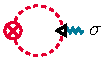
\includegraphics{0d/diagrams/SU2model0d-dUFlow_00203_1.pdf}}\end{gathered}
		-\frac{1}{2}\,\begin{gathered}\raisebox{-6pt}{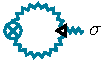
\includegraphics{0d/diagrams/SU2model0d-dUFlow_00024_1.pdf}}\end{gathered}\\
		&=\, - \frac{1}{2} \, \frac{N - 1}{\big[ r ( t ) + \frac{1}{\sigma} \, u ( t, \sigma ) \big]^2} \, \partial_\sigma \big[ \tfrac{1}{\sigma} \, u ( t, \sigma ) \big]\,\partial_t r ( t ) -\nonumber\\
		&\qquad\qquad\qquad\qquad\qquad\qquad- \frac{1}{2} \,  \frac{1}{\big[ r ( t ) +  \partial_\sigma u ( t, \sigma ) \big]^2} \, \partial_\sigma^2 u ( t, \sigma )\,\partial_t r ( t ) \\
		&=\, \dod{}{\sigma}\! \Bigg(
		\frac{1}{2}\,\begin{gathered}
\includegraphics{diagrams/SU2model0d-UFlow_00103_1.pdf}\end{gathered}
		+\input{0d/diagrams/SU2model0d-Uflow_00014_1.tex}
		\Bigg) \, .
	\end{align}
This corresponds to an interchange in the order of operations (evaluating the Wetterich equation on the background field configuration and taking derivatives \wrt{} the background field versus taking functional derivatives of the \frg{} equation and afterwards evaluating on the background field) and it is non-trivial (especially for flow equations for more complex models in higher dimensions and with truncation beyond \lpa{}) that the resulting equations are identical, \cf{} \cref{app:SU2}.

Before we turn to the fluid-dynamical interpretation of the conservation laws~\eqref{eq:conservation_law_u_rho} and \eqref{eq:conservation_law_u_phi}, we comment on the question whether one of the two formulations~\eqref{eq:conservation_law_u_rho} and \eqref{eq:conservation_law_u_phi} is preferable or if even others should be considered.
The answer to this question is not yet settled. 
From our present understanding, a formulation of the conservation equation in terms of $\sigma$ is preferable, for reasons of numerical implementability in the \fv{} scheme we use.
This is discussed at length in the context of the \pde{} \bcs{} for the \frg{} flow equation in \cref{subsec:boundary_conditions_finite_volume}.
Therefore, our discussion in the next sections is based on \cref{eq:conservation_law_u_phi}, and hence we identify $\sigma$ with the spatial coordinate $x$ and $u ( t, \sigma ) \equiv \partial_\sigma U ( t, \sigma )$ as the conserved quantity.\bigskip

The rest of this subsubsection is dedicated to the fluid-dynamical interpretation of the \frg{} flow equation \eqref{eq:conservation_law_u_phi}.
To this end, we split the flux (current) on the \rhs{} of the conservation law \eqref{eq:conservation_law_u_phi} and rewrite the whole equation in terms of an advection-diffusion equation, \cf{} \cref{eq:FVadsEq} and \cref{subsec:hydroAdvection,subsec:hydroDiffusion}, in one spatial dimension $x = \sigma$ and one temporal dimension $t$,
\begin{align}
	\partial_t u ( t, x ) + \dod{}{x} F [ t, x, u ( t, x ) ] = \dod{}{x} Q [ t, \partial_x u ( t, x ) ] \, .	\label{eq:advection_diffusion_equation_zero-dimensional}
\end{align}
The pionic contributions to the \frg{} flow,
\begin{align}
	F [ t, x, u ( t, x ) ] = \, & - \frac{1}{2} \, \frac{N - 1}{r ( t ) + \frac{1}{x} \, u ( t, x )}\, \partial_t r ( t ) = -\frac{1}{2}\,\begin{gathered}
\includegraphics{diagrams/SU2model0d-UFlow_00103_1.pdf}\end{gathered} \, ,\label{eq:advection_flux_pion_propagator}
\end{align}
are identified with a non-linear, position-dependent advection flux, while the contribution of the radial \sigmaMode{},
\begin{align}
	Q [ t, \partial_x u ( t, x ) ] = \, & + \frac{1}{2} \,  \frac{1}{r ( t ) + \partial_x u ( t, x )}\, \partial_t r ( t ) = \input{0d/diagrams/SU2model0d-Uflow_00014_1.tex}\, ,\label{eq:diffusion_flux_sigma_propagator}
\end{align}
corresponds to a non-linear diffusion flux.
We discussed conservation equations like \cref{eq:advection_diffusion_equation_zero-dimensional} in a \cfd{} context at length in our methodological introduction~\ref{sec:conservationLaws}.
In the following paragraphs we want to comment on the nature of the pionic/advective and radial $\sigma$/diffusive contributions using the established \cfd{} terminology.

\paragraph{Advection}\phantomsection\label{paragraph:conservative_form_advection}\mbox{}\\
If we ignore the contribution of the \sigmaMode{} for a moment (which \dash{} after rescaling \dash{} corresponds to the large-$N$ limit of the $O(N)$ model~\cite{Grossi:2019urj,Tetradis:1995br,Grossi:2021ksl,Steil:2021cbu}), we can rewrite the \lhs{} of \cref{eq:advection_diffusion_equation_zero-dimensional} as follows,
\begin{align}
	\partial_t u ( t, x )& + \dod{}{x} F [ t, x, u ( t, x ) ] =  0 \label{eq:advection_zero-dimensional} \\[.2em]
	\partial_t u ( t, x )& + \partial_u F [ t, x, u ( t, x ) ] \, \partial_x u ( t, x ) +\partial_x F [ t, x, u ( t, x ) ] = 0 \label{eq:advection_zero-dimensional_primitive}
\end{align}
This is a hyperbolic, non-linear advection equation for $u ( t, x )$, \cf{} \cref{eq:FVadsEqFonly}, and its accompanying \textit{primitive form}, \cf{} \cref{eq:FVFprimitive}, including an internal source term.
$\partial_u F [ t, x, u ( t, x ) ]$ is identified with the velocity of the characteristics (the local $u$-dependent flow velocity of the quantity $u$) and $\partial_x F [ t, x, u ( t, x ) ]$ acts like an $x$- and $u$-dependent internal source term.  
Hence $F [ t, x, u ( t, x ) ]$ is not purely advective nevertheless we will continue to refer to it as advection term.

The form of \cref{eq:advection_zero-dimensional} motivated our discussion of linear and non-linear advection equations in \cref{sububsec:LAEBBE} with the \laeq{} and \bbeq{} as instructive examples.
When compared to the \bbeq{} we notice that in our pionic \frg{} flow the local flow velocity is highly non-linear in $t$, $x$ and $u$ and explicitly reads
\begin{align}
	\partial_u F [ t, x, u ( t, x ) ] = \, & \frac{1}{2}\,\frac{ N - 1 }{x \, \big[ r ( t ) + \frac{1}{x} \, u ( t, x ) \big]^2}\,\partial_t r ( t ) \, .	\label{eq:advection_velocity}
\end{align}
Considering for example the exponential regulator shape function \eqref{eq:exponential_regulator}, one finds that the advection velocity $\partial_u F [ t, x, u ( t, x ) ]$ is always negative (positive) for $x > 0$ ($x < 0$).
In a fluid-dynamical picture, this means that the conserved quantity $u ( t, x )$ is always propagated from larger values of $|x|$ towards the point $x = 0$ by advection.
Furthermore, the closer the fluid $u ( t, x )$ is to $x = 0$, the faster the fluid moves, due to the factor $\frac{1}{x}$.
Since $u ( t, x )$ is antisymmetric in $x$, because of the $O(N)$ symmetry of $U ( t, \vec{\varphi} \, )$, this implies that ``waves'' of positive and negative $u ( t, x )$ collide with huge velocity at $x = 0$ and annihilate.
At large $|x|$, the fluid velocity tends to zero.

We also observe that the advection velocity \eqref{eq:advection_velocity} is proportional to the number of pions, $ N - 1 $.
Hence, in the large-$N$ limit the system, discussed at length in \cref{subsec:0dLargeN}, is completely advection driven, while for small $N$ the diffusive contributions \eqref{eq:diffusion_flux_sigma_propagator} gain in importance.
In the case $N = 1$, discussed at length in \cref{subsec:0dO1Entropy}, there is no advection at all and the dynamics of the fluid $u ( t, x )$ is purely diffusive.

At this point we want to remind the reader of the general properties and features of non-linear advection equations \dash{} like shock formation, (numerical) entropy production, and irreversibility \dash{}
discussed in general in \cref{subsec:hydroAdvection}.
Naturally those properties also play an important role in the dynamics of \frg{} flows, which we will discuss in the following conceptually and also using explicit examples.

\paragraph{Diffusion}\phantomsection\label{paragraph:conservative_form_diffusion}\mbox{}\\
Next, we turn to the contribution of the radial \sigmaMode{} to the \frg{} flow. 
We find that it enters the conservation law \eqref{eq:advection_diffusion_equation_zero-dimensional} as a non-linear diffusion flux \eqref{eq:diffusion_flux_sigma_propagator}, because it is overall of second-order in spatial derivatives of $u ( t, x )$. 
The characteristic property of diffusive processes is that they transport a quantity, in this case $u ( t, x )$, from regions where its density or concentration is high to regions where it is low~\cite{LeVeque:1992,LeVeque:2002,RezzollaZanotti:2013,Ames:1992}, \cf{} \cref{subsec:hydroDiffusion}.
Diffusive processes are therefore usually important in regions of high gradients and smear out cusps, shocks \etc{}, which might form via advection.
Besides this, diffusive processes are generically undirected, which is also the case for the diffusion flux \eqref{eq:diffusion_flux_sigma_propagator} which propagates the quantity $u ( t, x )$ in both directions, depending on the local gradients of $u ( t, x )$, which is especially relevant for models in their symmetry-broken phase with rather weak advection (small $N$). 
The effective transport velocities via diffusion are usually much slower than those via advection, which is, due to the non-linearity, not necessarily true for \frg{} flow equations.
We discussed the \heq{} as an archetypal linear diffusion equation at length in \cref{paragraph:HE}.
The diffusion flux \eqref{eq:advection_diffusion_equation_zero-dimensional} can be formulated as a non-linear time-dependent realization of the heat equation.
By performing the spatial derivative in the advection-diffusion equation \eqref{eq:advection_diffusion_equation_zero-dimensional} for the purely diffusive ($N = 1$) case, one finds
\begin{align}
	\partial_t u ( t, x ) = \, & \alpha[t,\partial_x u ( t, x )] \, \partial_x^2 u ( t, x ) \, ,\label{eq:0ddifprim}
\end{align}
where
\begin{align}
	\alpha[t,\partial_x u ( t, x )] \equiv - \frac{\tfrac{1}{2} \, \partial_t r ( t )}{[ r ( t ) + \partial_x u ( t, x ) ]^2} \, ,	\label{eq:diffusion_coefficient}
\end{align}
plays the role of a non-linear time-dependent, strictly positive \dash{} parabolic \dash{} diffusion coefficient. 
The positivity of the diffusion coefficients ensures that $u ( t, x )$ is only dispersed and never accumulates locally, \ie{}, that $u ( t, x )$ tends to equilibrate towards a linear function in space. 
A positive diffusion coefficient also ensures stability and uniqueness of (numerical) weak solutions, as discussed in the beginning of \cref{subsec:hydroDiffusion}.

Directly comparing these findings with the \he{}, we can already qualitatively predict the behavior of the diffusion transport for the \frg{} flow of $u ( t, x )$, as long as $N$ is small and the system is diffusion-dominated.
At a constant \rgtime{} $t$, we find that the diffusion coefficient is much larger in regions where the gradient $\partial_x u ( t, x )$ is negative with a large absolute value, compared to regions where it is positive, because in the first case the denominator of \cref{eq:diffusion_coefficient} is smaller than in the second case.
This plays a crucial role for systems that involve symmetry breaking, where $\partial_x u ( t, x )$ is negative for at least some small $|x|$, while asymptotically for $|x| \rightarrow \infty$ the sign of $\partial_x u ( t, x )$ is always positive.
Hence, for diffusion-dominated problems in \frg{} flow equations (small number $N$ of pions), the symmetry restoration is driven by the negative gradients $\partial_x u ( t, x )$ at small $|x|$.
Furthermore, we find that for $t \rightarrow \infty$, the numerator of the diffusion coefficient \eqref{eq:diffusion_coefficient} tends to zero such that the diffusion stops, the system equilibrates and the dynamics freezes, even though there are still gradients in $u ( t, x )$.
This would not happen for the linear \he{} with its constant diffusion coefficient.
The same is true for $t = 0$, where the diffusion coefficient is suppressed by $1/\Lambda$.

\paragraph{Irreversibility and entropy production}\phantomsection\label{paragraph:conservative_form_entropy}\mbox{}\\
In a fluid-dynamical setting, it is very easy to understand the role of the radial \sigmaMode{}: Due to its diffusive character, it is directly responsible for the irreversibility of the \grg{} flow and \rg{} transformations in general. 
Diffusion is a particular example of a dissipative process, which is irreversible and increases the entropy of the system\footnote{%
	Interestingly, \ccite{Zamolodchikov:1986gt} comes to the same conclusion arguing in reverse order:
	``Some of the information on the ultraviolet behavior of the field theory is lost under renormalization transformations with $t>0$, since in the field theory it is not legitimate to examine correlations at scales smaller than the cutoff.
	We would therefore expect that a motion of the space $Q$ [a change of the set of all couplings] under the influence of the renormalization group would become an `irreversible' process, similar to the time evolution of dissipative systems.''
	We remark that also \ccite{Zumbach:1994vg} stated that a term of second-order in field space derivatives in related \rg{} flow equations ``[\ldots] corresponds to a dissipation in the flow and is responsible for the semi-group property of the \rg{}''.%
}.
The dissipative and irreversible character can be seen as a ``thermodynamic'' version of the irreversible Kadanoff block-spin transformations~\cite{Kadanoff:1966wm,Wilson:1979qg,Delamotte:2007pf}.
Hence, the dissipation clearly singles out the \rgtime{} $t$ as a temporal direction, because it introduces a ``thermodynamic arrow of time'' and ``thermodynamic time asymmetry'' via entropy production~\cite{Lebowitz:2008}.
This also explains why our definition \eqref{eq:def_rg_time}:
\begin{align}
	&t \equiv - \ln \big( \tfrac{k}{\Lambda} \big) =  \ln \big( \tfrac{\Lambda}{k} \big) \, ,	\qquad	t \in [ 0, \infty ) \, .	\label{eq:rg-time-scale}
\end{align}
is a natural choice for a temporal coordinate also in higher dimensions, see also \ccite{Hasenfratz:1985dm,Zumbach:1993zz,Zumbach:1994vg,Zumbach:1994kc,Grossi:2019urj}.

Interestingly, the irreversibility and the dissipative character of the system is lost if one does not include the full field-dependence of the effective potential in the flow equation, but instead uses a truncated system like the Taylor expansion \eqref{eq:example_vertex_expansion}.
Then, the system \eqref{eq:example_vertex_expansion} of coupled \odes{} for the vertices can theoretically be integrated in either direction in \rgtime{}, as long as it consists of a finite number of couplings\footnote{%
	In momentum space this enables an integration to higher energy scales, which corresponds to a reversion of the coarse-graining in position space.
	More generally speaking, this implies that it is possible to resolve the microphysics from the macrophysics.
	Both are physically not possible and solely an artifact of the truncation.%
}.
The most extreme examples are the \rg{} flows of one single $t$-dependent coupling, \eg{}, the quartic coupling of $\phi^4$ theory or the \qcd{} beta function~\cite{Politzer:1973fx,Gross:1973id,Gross:1973ju,Gross:1974cs}, see also the textbooks~\cite{ZinnJustin:2002ru,Peskin:1995ev}.
Here the integration to both higher and smaller \rgscales{} is possible, which is the well-known result for the universal one-loop beta function and is an artifact of the restriction (truncation) to a finite number of couplings~\cite{Wilson:1979qg}.
However, this reversibility of \rg{} transformations is not possible for the field-dependent effective potential, which is obvious from the advection-diffusion equation~\eqref{eq:advection_diffusion_equation_zero-dimensional}, where entropy increases and the information about the \ic{} in the \uv{} cannot be recovered from the \ir{} anymore.

This point of view was already shared, presented, and discussed by K.~G.~Wilson:
In \nbccite{Wilson:1979qg} he pointed out the differences between his ``coarse-graining'' version of the \rg{}, which is also applicable in highly non-perturbative regimes, and the \rg{} flow equations used by C.~Callan, K.~Symanzik, M.~Gell-Mann, F.~Low, G.~t'Hooft, S.~Weinberg, H.~Georgi, D.~Politzer and others to calculate the running of a single (or small number of) coupling constants, which solely describes a system correctly in a perturbative regime.

The irreversibility of the \frg{} flow and entropy production is also directly related to the presence of discontinuities in the solution, which can arise from the advective contributions to the flow.
As shown in \ccite{Aoki:2017rjl,Grossi:2019urj,Grossi:2021ksl,Steil:2021cbu} for the large-$N$ limit, a shock wave arises when the weak solution of the \pde{} is multi-valued. 
The correct solution is usually constructed by means of the Rankine-Hugoniot condition~\cite{Rankine:1870,Hugoniot:1887,LeVeque:1992,LeVeque:2002,RezzollaZanotti:2013,Ames:1992}.
This would lead to ambiguities when one tries to invert the flow (integrating backwards in time) in the presence of a shock.
Hence, shock formation is an irreversible process and produces entropy.
In summary, these are further strong arguments why the assumption of expandability of the effective average action in terms of vertices as well as the truncation of the system should in general be considered with care.

Therefore, it would be extremely interesting to explicitly construct an entropy function for the flow equation, \ie{}, a quantity that is either non-decreasing or non-increasing under the \rg{} transformations during the \frg{} flow (depending on the sign convention), and that is a functional of the quantity $u ( t, x )$.
The entropy for the flow equation will be a helpful instrument to design a stable numerical scheme for generic truncations~\cite{LeVeque:1992,LeVeque:2002,RezzollaZanotti:2013} and will also highlight general properties of the \grg{} flow.
In this context we also have to mention the recent publication~\cite{Cotler:2022fze} by J. Cotler and S. Rezchikov who were able to interpret the Polchinski equation as an ``optimal transport gradient flow of a field-theoretic relative entropy'' thus establishing a firm and explicit connection between an information-theoretic entropy and (F)RG flows.

Additionally, a numeric entropy (function) might provide a direct link to $\mathcal{C}$-/$\mathcal{A}$-theorems~\cite{Zamolodchikov:1986gt,Banks:1987qs,Cardy:1988cwa,Osborn:1989td,Jack:1990eb,Komargodski:2011vj,Curtright:2011qg,Rosten:2010vm}, which state that in certain \qfts{} there exists some positive real function $\mathcal{C} ( \{ g_i \} , t )$, which depends on all coupling constants of the QFT and which is monotonically increasing\footnote{%
	It can also be defined as a monotonically decreasing function.
	This flip of sign corresponds to the difference of the mathematicians' and physicists' definition of entropy.
	We chose to the ``thermodynamic convention'' of increasing entropy for this and subsequent publications.
} during \rg{} flows (transformations), while it stays constant at (critical) fixed points,
	\begin{align}
		\dod{}{t} \mathcal{C} ( \{ g_i \} , t ) \geq 0 \, .
	\end{align}
Here, $\{ g_i \}$ denotes the set of all (possibly infinitely many) dimensionless coupling constants.
In contrast to previous formulations~\cite{Haagensen:1993by,Generowicz:1997he,Forte:1998dx,Codello:2013iqa,Codello:2015ana,Becker:2014pea,Becker:2016zcn}, a non-local version, which is directly linked to the numerical entropy function (similar to versions presented in \ccite{Zumbach:1993zz,Zumbach:1994vg,Rosten:2010vm} for related field-dependent flow equations), would not rely on expandability in the couplings or vertices and could naturally display the dissipative character of \rg{} transformations, which was already described by \ccite{Zamolodchikov:1986gt,Zumbach:1994vg}.
Fixed-point solutions of the \frg{} flow would directly correspond to steady-state or thermal-equilibrium solutions~\cite{LeVeque:1992} in the fluid-dynamical picture\footnote{%
	This actually brings up the interesting question whether previous studies about global fixed-point solutions for field-dependent flow equations, which seemed to deliver interesting results, \eg{}, \ccite{Borchardt:2015rxa,Zumbach:1994vg,Yabunaka:2018mju}, should be reanalyzed from the fluid-dynamical steady-flow perspective, especially regarding their interpretation and the spatial discretization methods~\cite{LeVeque:1992}.
}.
A caveat at this point is that a $\mathcal{C}$ function is based on the rescaled dimensionless \rg{} flow equations.
Hence, also a numerical entropy should be formulated in this framework, if one seeks a direct link to a $\mathcal{C}$ function.
The dimensionless flow equations in the \lpa{} can be recast in terms of conservation laws, which might be a good starting point.

An explicit discussion of (numerical) entropy for the zero-dimensional $O(1)$ model as well as possible links to $\mathcal{C}$ functions is discussed in great detail in \cref{subsec:0dO1Entropy}.
The situation for the $O(N)$ model in the limit $N\rightarrow\infty$ is discussed in \cref{subsec:0dLargeN}.
The construction of an explicit (numerical) entropy has proven to be elusive in the case of finite $N>1$ for the $O(N)$ model~\cite{Koenigstein:2021rxj,Steil:2021cbu} due to the explicit position-dependencies in \cref{eq:conservation_law_u_phi} and \eqref{eq:conservation_law_u_rho} and the related internal source terms, \cf{} \cref{eq:advection_zero-dimensional}.

\paragraph{Generalizations}\phantomsection\label{paragraph:conservative_form_generalizations}\mbox{}\\
At this point we want to briefly comment on the generalization of the fluid-dynamical picture to \frg{} flow equations in higher-dimensional \qfts{}, systems with more (field-dependent) couplings, and \frg{} flow equations that involve fermions.

In higher-dimensional \qfts{}, the fluid-dynamical interpretation of the \frg{} flow of the effective potential survives, see for example \ccite{Grossi:2019urj,Grossi:2021ksl,Koenigstein:2020Talk,Stoll:2021ori,Ihssen:2022xkr,Ihssen:2023xlp} and especially \cref{chap:GN}.
In zero dimensions, $t$ merely parametrizes some dimensionless (mass-like) scale $r ( t )$, see \cref{eq:exponential_regulator}. 
In contrast, in higher dimensions, the \rgtime{} is defined as the negative logarithm of the ratio between the \rg{} momentum scale $k$ and the \uv{} reference scale $\Lambda$, see \cref{eq:rg-time-scale}.
The fluxes gain further $t$-dependent prefactors via the momentum integrals of the trace in the Wetterich equation.
This leads to a different time scaling but does not affect the overall discussion. 
The inclusion of further field-independent but scale-dependent couplings (such as a scale-dependent Yukawa coupling) adds \odes{} to the advection-diffusion equation for the effective potential, which does not spoil its conservative fluid-dynamical character.
It is currently investigated by us and collaborators~\cite{Ihssen2020,Grossi:2021ksl,Ihssen:2022xkr,Ihssen:2023nqd,Ihssen:2023xlp} whether the inclusion as well as the conservative formulation of further field-dependent couplings (such as a field- and scale-dependent wave-function renormalization $Z ( t, \vec{\varphi} \, )$ in higher-dimensional models) is possible.
In any case, simply adding fermions in the \lpa{} does not destroy the fluid-dynamical character of the \frg{} flow equation at all: On the level of the \lpa{} for the \frg{} flow equation of the effective potential, the contributions from fermion loops can be interpreted as a source/sink term, which only depends on $\sigma$, \ie{}, the spatial position $x$.
We discuss such fermionic source/sink terms in zero dimensions in \cref{sec:0dSU2} and in non-zero, \ie{}, $1\dimSpacer + \dimSpacer 1=2$ dimensions, at zero and non-zero temperature and especially quark chemical potential in \cref{chap:GN}.
Another possible generalization concerns models with more than one invariant of the underlying symmetry group of the model and respective condensation directions in field space, see, \eg{}, \ccite{Strodthoff:2011tz,Mitter:2013fxa,Rennecke:2016tkm,Lakaschus:2020caq,Fukushima:2010ji,Fejos:2020lli}.
Here, the fluid-dynamical framework should still be applicable.
However, a suitable identification of a complete basis of field space directions with ``spatial directions'' of the fluid-dynamical problem and a clear separation of the single contributions into advection, diffusion, and source terms might be challenging and calls for future investigations \dash{} especially when it comes to an actual numerical implementation.
For first attempts of generalizing our findings to a quark-meson-diquark model, we refer to \ccite{Lakaschus:2021ewd}.

Summarizing we find that the fluid-dynamical interpretation of flow equations has tremendous benefits, because it allows for a rather intuitive understanding of the dynamics of the system. Furthermore, it allows for a novel, physically intuitive interpretation of the \frg{} flow and provides an understanding of its irreversibility.
Finally, it opens up the opportunity to employ extremely powerful numerical tools from \cfd{}.

\subsubsection{Boundary conditions and computational domain}\label{subsec:boundary_conditions_finite_volume}
\begin{disclaimer}
	This subsubsection follows the discussion presented in Sec.~IV.D of \nbccite{Koenigstein:2021syz}.
\end{disclaimer}
In the form of the conservation laws \eqref{eq:conservation_law_u_rho} or \eqref{eq:conservation_law_u_phi}, the \frg{} flow equation \eqref{eq:flow_equation_effective_potential} is a non-linear \pde{} which has contributions of parabolic (diffusion terms) as well as hyperbolic (advection terms) nature.
In this subsubsection, we specify the \bcs{} for Eqs.~\eqref{eq:conservation_law_u_rho} or~\eqref{eq:conservation_law_u_phi} in field space (the effective spatial $x$-direction).

For (non-linear) \pdes{} of hyperbolic and parabolic type, the spatial \bcs{} are needed (in addition to the \ic{}) to make finding a (weak) solution a well-defined problem, \cf{} \cref{subsec:hydroAdvection,subsec:hydroDiffusion}.
We are dealing with a \textit{Cauchy} or to be even more specific an \textit{initial-boundary-value} problem.
Thus, without explicitly specifying the \bcs{}, \eg{}, of Neumann- or Dirichlet-type, as well as the \ics{}, the problem of finding a unique (weak) solution is actually ill-posed and therefore impossible to solve \dash{} a well-known mathematical fact with particular and severe implications in, \eg{}, classical electrodynamics~\cite{Jackson:1998nia}, fluid dynamics~\cite{BuckleyLeverett:1942}, soliton and instanton solutions of classical field equations~\cite{Rajaraman:1982is,Shifman:1994ee}, general relativity~\cite{Weinberg:1972kfs,Misner:1974qy,Ryder:2009zz}, and other fields of research.
This \dash{} unsurprisingly \dash{} also holds true for the \frg{}. 
However, explicit \bcs{} and especially their numerical implementation are rarely discussed in \frg{} literature, with, \eg{}, \ccite{Caillol:2012zz,Pangon:2009pj,Pangon:2010uf,Codello:2013iqa} as notable exceptions before the advent of \cfd{} methods for the \frg{}~\cite{Grossi:2019urj,zerod1,zerod2,zerod3,Ihssen2020,Stoll:2021ori,Grossi:2021ksl,Ihssen:2022xkr,Ihssen:2023nqd,Ihssen:2023xlp}.

For the derivative of the effective potential $u ( t, \sigma )$, we find that the spatial \bcs{} must be imposed at $\sigma = \pm \infty$, because the field space domain of $u ( t, \sigma )$ is given by $\Reals{}$.
Thus, when considering the flow equation on the non-compact domain $( - \infty, \infty )$ the problem represents a \textit{pure initial-value/Cauchy problem}~\cite{Ames:1992,LeVeque:1992,LeVeque:2002} and, given the asymptotics of the flow equation and the \ic{}, explicit \bcs{} at $\sigma\rightarrow\pm\infty$ are not required.
However, spanning a non-compact computational interval from $ - \infty$ to $ + \infty$ is practically impossible on a finite computational grid.
A possible solution is a compactification~\cite{Borchardt:2016pif} of $\Reals{}$ to the interval $[ - 1, + 1 ]$, via a suitable mapping $\sigma \mapsto x ( \sigma )$ usually supplemented with a mapping $u \mapsto v(u)$ rendering $v$ finite on~${[ - 1, + 1 ]}$.
Another popular solution is a truncation of the computation interval at a large value $\sigma_\text{max} \sim x_\mathrm{max}$ with a suitable \bc{}~\cite{Pangon:2009pj,Caillol:2012zz,Borchardt:2015rxa,Borchardt:2016pif}.
We will return to this issue below.

In any case, one of the boundaries at spatial infinity can already be replaced by a finite value by making use of the $O ( N )$ symmetry of the potential $U ( t, \vec{\varphi} \, )$ and the flow equations, which implies a \ZII{} antisymmetry of $u ( t, \sigma ) = \partial_\sigma U ( t, \sigma )$,
\begin{align}
	U ( t, \sigma ) = U ( t, - \sigma ) \qquad\Longleftrightarrow\qquad	u ( t, \sigma ) = - u ( t, - \sigma ) \, .	\label{eq:anti-symmetry_small_u}
\end{align}
This reduces the spatial domain to the half-open interval $\sigma \in [ 0, + \infty )$, but now we need an additional artificial \bc{} at $\sigma = 0$, see, \eg{}, \ccite{Pangon:2009pj}.
In previous studies, the use of the $O(N)$ symmetry was usually implemented right from the beginning by replacing the variable $\vec{\varphi}$ by the $O(N)$ invariant $\varrho = \tfrac{1}{2}\,\vec{\varphi}^{\, 2}$, whose domain is already by definition $[ 0, \infty )$.\footnote{%
	In any case, independent of the implementation of the \bc{} itself, one should make use of symmetries of the flow equations in numerical implementations.
	First of all, this leads to a reduction of the number of computational grid points in spatial direction, while keeping the spatial resolution fixed, which significantly speeds up the calculations (independently of the specific numerical method for spatial discretization).
	An additional consequence is the reduction of numerical errors: It is highly unlikely that the numerical errors are symmetric in $x$, if a symmetric interval around $x=\sigma=0$ is used.
	This might lead to an artificial breaking of the \ZII{} antisymmetry by unbalanced numerical errors.
	Although these errors might be tiny and almost negligible they can be easily circumvented by exploiting the symmetries.
	Using the symmetries of a problem is a standard procedure in practical computations and of particular importance in, \eg{}, numerical fluid dynamics and numerical (general) relativity, see \ccite{Baumgarte2010Jun,Alcubierre2008,Grandclement:2007sb,Gourgoulhon:2007ue}.%
} 
In this case one has to define 
\begin{align}
	u ( t, \varrho ) \equiv \partial_\varrho U ( t, \rho ) = \tfrac{1}{\sigma} \, \partial_\sigma U ( t, \sigma ) = \tfrac{1}{\sigma} \, u ( t, \sigma ) \, ,
\end{align}
to obtain a flow equation for $u ( t, \varrho )$ in a manifestly conservative form, see \cref{eq:conservation_law_u_rho,eq:conservation_law_u_phi}.
Before returning to the remaining \bc{} at $+ \infty$, we first consider the newly introduced artificial \bc{} at ${x = \sigma =0}$ or, correspondingly, at $ \varrho=0$.

\paragraph{The boundary condition at $\sigma = 0$}\phantomsection\label{paragraph:BC0}\mbox{}\\
At first sight it might be appealing to formulate the whole problem \dash{} the conservation equation and the \bc{} at $\sigma = 0$ \dash{} in the variable $\varrho$.
However, we believe that a formulation in $\sigma$ is more suitable and easier to implement in our numerical \fv{} setup.\footnote{%
	We do not claim that it is impossible to formulate well-defined discrete \bcs{} in $\varrho$ at $\varrho = 0$, as can be seen for example in \ccite{Grossi:2019urj,Grossi:2021ksl,Steil:2021cbu} for the specific case of the large-$N$ limit of the $O(N)$ model and generalizations to finite $N$~\cite{Ihssen:2022xkr,Ihssen:2023xlp}. 
	However, we were not able to provide a suitable discretization of the \bc{} at $\varrho = 0$ in the implementation of the \fv{} method for flow equations that include diffusion via the radial \sigmaMode{}.
}
A key feature of (non-linear) hyperbolic/parabolic conservation equations is that their weak solutions may exhibit non-analyticities in the form of shock and rarefaction waves \etc{}, which manifest themselves in the solution in cusps or discontinuities in spatial direction during the time evolution, \cf{} \cref{subsec:hydroEuler}.
These effects can develop during the time evolution even if the \ic{} is smooth/analytic, see, \eg{}, \ccite{KTO2-0,Chen:2001,Bateman1915,Burgers1948,LeVeque:1992,LeVeque:2002,Borchardt:2016pif} and our discussion of the \bbeq{} in \cref{paragraph:BBE}.
As demonstrated in \ccite{Aoki:2017rjl,Wink:2020tnu,WinkHirschegg,Grossi:2019urj,Grossi:2021ksl,Ihssen2020,Stoll:2021ori,Ihssen:2022xkr,Ihssen:2023xlp} this also holds for \frg{} flow equations, where non-analyticities are inherent properties of the effective \ir{} potential $U ( t_\mathrm{IR}, \sigma )$.
These statements are also true for the point $\sigma = 0$, where $U ( t, \sigma )$ and $u ( t, \sigma )$ do not need to be analytic, see \cref{subsubsec:sc4}.
Hence, there might be a scenario where the potential $U ( t, \sigma )$, although it is symmetric in $\sigma$, has a cusp at $\sigma = 0$, which would correspond to a jump in a weak solution for $u ( t, \sigma ) = \partial_\sigma U ( t, \sigma )$ at $\sigma = 0$.
If formulated in $\varrho$, any scenario (analytic or non-analytic at $\sigma = 0$) merely corresponds to some arbitrary value for $u ( t, \varrho ) = \partial_\varrho U ( t, \varrho )$ at $\varrho = 0$, which seems to be of great advantage, because one does not have to deal with possible discontinuities in the conserved quantity $u$.
Furthermore, the problematic factors of $\frac{1}{\sigma}$ in the pion propagator and the advection flux \eqref{eq:advection_flux_pion_propagator}, which are diverging at $\sigma = 0$, can be avoided when formulating the flow equations in $\varrho$.

Nevertheless, a problem with the variable $\varrho$ becomes apparent when turning to the discretized form of $u$ within the \fv{} scheme introduced in \cref{sec:conservationLaws} and specifically \cref{subsec:hydroKT}: \fv{} methods (and also other discretization schemes) usually require ghost cells at the boundaries of the computational domain, since the in- and out-flows for the \ith{i} cell are calculated from the cell averages $\bar{u}$ of its neighboring cells, \cf{}\ \cref{eq:kt_stencil}.
However, initially these values are not specified for the cells at the boundaries of the computational domain.
Thus, artificial ghost cells must be introduced and the numerical values for $\bar{u}$ in these ghost cells have to be implemented by hand or reconstructed from the cells within the computational domain in accordance with the \bcs{}~\cite{LeVeque:1992,LeVeque:2002}, \cf{} \cref{subsec:hydroAdvection,subsec:hydroDiffusion} and \cref{eq:BClinExt,eq:BCperiodic,eq:heICS1DBCFV,eq:heICS2NBCFV,eq:eulerReflectiveBC}.
In the second-order formulation of the one-dimensional \kt{} scheme one needs two ghost cells at each of the two spatial boundaries, \cf{} \cref{eq:kt_stencil}.

However, implementing ghost cells for $u ( t, \varrho )$ at $\varrho = 0$ is conceptually difficult, because these ghost cells must be centered at negative values for $\varrho$ outside the computational domain $[ 0, \infty)$, which by definition do not exist due to the positivity of $\varrho = \tfrac{1}{2}\,\sigma^2$.
\Apriori{}, it is therefore not clear how numerical values $\bar{u} ( t, \varrho_i )$ should be assigned to ghost cells at negative $\varrho_i$, because symmetry arguments cannot be applied anymore.

Furthermore, it is also not a feasible option to move the ghost cells to positive values of $\varrho_i$, such that the point $\varrho = 0$ is no longer part of the computational domain.\
Namely, having ghost cells centered at small but positive $\varrho_i$ implies that one has to extrapolate the numerical values $\bar{u} ( t, \varrho_i )$ to these ghost cells and to the point $\varrho = 0$ from the other ordinary cells of the computational domain.
However, the functional behavior of $u ( t, \varrho )$ is unknown for small $\varrho$ and is actually exactly what we want to calculate in the first place by solving the \pde{}.
Thus, any extrapolation at small $\varrho$ can only be considered an educated guess.
It is especially dangerous, because the physical point will be part of the extrapolated ghost cells if it is located at $\varrho = 0$, which is the case for all models in their symmetric phase~\cite{Stoll:2021ori}, irrespective of the dimensionality of space-time.
Consequently, extrapolation errors at the physical point have the potential to spoil the numerical values of all \nptFunctions{}, which are calculated at the physical point via derivatives of $u$ and contain the physics of the model.
Even if the physical point is at finite non-zero $\varrho$ far away from the ghost cells and the boundary at $\varrho = 0$, any kind of extrapolation at small $\varrho$ leads to numerical errors, because the diffusive contributions of the radial \sigmaMode{} will propagate this information from smaller to larger $\varrho$ and hence to the physical point.
Similar problems in formulating appropriate \bcs{} at $\varrho = 0$ also exist in other discretization schemes like finite-difference or finite-element methods.

There is one exception to this conclusion: In the large-$N$ limit of the $O(N)$ model the flow equation for $u$ reduces to a pure advection equation.
Studying the characteristic velocities, which are given by $\partial F/\partial u$, respectively, see \cref{eq:advection_velocity}, we find that these cannot change their sign, and information (or the conserved quantity $u$) is always propagated via advection in the direction of smaller $\varrho$ or $|\sigma|$.
In this scenario, ghost cells can be positioned at negative $\varrho_i$ and the corresponding cell averages $\bar{u}_i$ in the ghost cells can take any numerical value since information from the ghost cells is never propagated back into the computational domain and cannot cause any errors, \cf{}\ \ccite{Grossi:2019urj,Grossi:2021ksl,Steil:2021cbu} and especially \cref{subsec:0dLargeN}.
Shifting the ghost cells into regions of positive $\varrho$ is still not suitable for the reasons already discussed above.\bigskip

In order to avoid all these difficulties when formulating the problem in the variable $\varrho$, we suggest a formulation in $\sigma$ and an implementation of the \bc{} at $\sigma = 0$.
The key argument for using $\sigma$ instead of $\varrho$ is that positioning ghost cells at negative $\sigma$ poses no problem at all, since negative $\sigma$ exist in the first place. 
Furthermore, it is clear how the cell averages $\bar{u} ( t, \sigma_i )$ in the ghost cells have to be chosen: Using the antisymmetry \eqref{eq:anti-symmetry_small_u}, one merely has to mirror the last physical cells of the computational domain at $\sigma = 0$ to the ghost cells (including a flip in sign).
The only issue that requires careful consideration is the choice of the position of the first physical cell $x_0$ next to $\sigma = 0$: The flux term of our \pde{} contains factors $\frac{1}{\sigma}$ via the pion propagators, which diverge if evaluated at $\sigma = 0$.
Therefore, we must avoid evaluating the fluxes $F [ t, x, u ( t, x ) ]$ at $x = \sigma = 0$.
However, inspecting the \kt{} scheme, we find that the fluxes as well as the Jacobian $ \frac{\partial F[u]}{\partial u}$ must only be evaluated at the cell boundaries $x_{j \pm \ttfrac{1}{2}}$, \cf{}\ \cref{eq:FVajp12} and \eqref{eq:definition_h_kt_scheme}.
Consequently, the natural choice for the position of the cell center $x_0$ of the first physical cell in the computational domain is at $x = \sigma = 0$, such that the in- and out-fluxes of this cell are evaluated at $x_{\pm \ttfrac{1}{2}}$, which is not problematic.
Incidentally, this automatically cures the problem of the possibility of non-analyticities in $u ( t, \sigma )$ at $\sigma = 0$: Even if $u ( t, \sigma )$ is discontinuous at $\sigma = 0$ we do not run into problems, because all numerical calculations are performed on the level of cell averages $\bar{u} ( t, \sigma_i )$.
The cell average of an antisymmetric function in a cell that is centered at $\sigma = 0$ must always vanish identically, independent of all other properties of the function, see also \ccite{Pangon:2009pj,Pangon:2010uf}.

\halfWidthFigure%
	[t]% Placement
	{0d/figures/boundary_condition_finite_volume.pdf}% Graphics
	[]% Sublabels
	{%
		Second-order accurate \fv{} implementation of the spatial \bc{} for $u ( t, x)$ or $\bar{u}_i (t)$, respectively, at $x = 0$ using \cref{eq:phi0BC0}. 
		We use the fact that $u ( t, x )$ is an odd function in $x$ by positioning the first computational cell $x_0$ at $x = 0$, such that the cell average is exactly zero, $\bar{u}_0 = 0$, which is true for $u (t, x)$ which are continuous (blue-dashed) as well as discontinuous (green-solid) at $x = 0$.
		Corresponding cell averages $\bar{u}_i$ are depicted as horizontal bars (magenta-dashed and yellow-solid).
		This \bc{} can be generalized to lower- and higher-order accurate \fv{} schemes as well as finite-difference or finite-element schemes.
		\fromFig{3}{zerod1}%
	}%Caption
	{fig:numerical_boundary_conditions_phi=0}%Label
In summary, we switch from the open computational interval $ ( - \infty, + \infty ) $ to the half-open computational interval $ [ 0, + \infty ) $ by means of the \ZII{} (anti-)symmetry using
\begin{align}
	\bar{u}_{-2} ( t ) = - \bar{u}_{2} ( t )\,,\quad \bar{u}_{- 1} ( t ) = - \bar{u}_{1} ( t )\,,\quad \bar{u}_0 ( t ) = 0\,,
	\label{eq:phi0BC0}
\end{align}
for the cell averages in the ghost cells left of $x_0 = 0$ and in the cell at $x_0$ itself.
This construction is visualized in \cref{fig:numerical_boundary_conditions_phi=0} for exemplary continuous and discontinuous initial conditions. 
It effectively corresponds to reflective \bcs{} frequently imposed in \cfd{}~\cite{LeVeque:1992,LeVeque:2002,SpringelLectureNotes}, see, \eg{}, \cref{eq:eulerReflectiveBC}.

\paragraph{The boundary condition at $\sigma \rightarrow \infty$}\phantomsection\label{paragraph:BCinf}\mbox{}\\
Now we return to the \bc{} at $\sigma \rightarrow + \infty$.
\WlogA{} we discuss the interval ${\sigma \in [ 0, + \infty )}$ since the situation in $\sigma \in (- \infty,0]$ follows from \ZII{} antisymmetry of $u(t,\sigma)$.

We have already argued that there are no real \bcs{} at spatial infinity on a non-compact domain.
The behavior of $u$ at $\sigma \rightarrow \infty$ is rather given by the asymptotics of the Wetterich equation, which makes the \pde{} an pure initial-value problem.
The \bc{} at spatial infinity is actually fixed implicitly: As long as the initial potential $U ( t = 0, \sigma )$ is bounded from below and grows faster than $\sigma^2$ for $\sigma \rightarrow \infty$ both pion and sigma propagator tend to zero for sufficiently large $\sigma$, such that the \rhs{} of the \pde{} \eqref{eq:conservation_law_u_phi} vanishes during the entire \frg{} flow.
In the fluid-dynamical picture this corresponds to vanishing advection~\eqref{eq:advection_flux_pion_propagator} and diffusion fluxes~\eqref{eq:diffusion_flux_sigma_propagator} at $\sigma \rightarrow \infty$, which is a zero-influx \bc{} for $u ( t, \sigma )$.
The derivative of the effective potential $u ( t, \sigma )$ is therefore fixed to its initial value $u ( t = 0, \sigma )$ at $\sigma \rightarrow \infty$.

The limiting case, when the asymptotic behavior of the \uv{} initial potential is quadratic,
\begin{align}
	\lim\limits_{\sigma \rightarrow \infty} U ( t = 0, \sigma ) \sim \sigma^2 \qquad\Longleftrightarrow\qquad	\lim\limits_{\sigma \rightarrow \infty} u ( t = 0, \sigma ) \sim \sigma \, ,
\end{align}
is more delicate.
In this case, the advection and diffusion fluxes \eqref{eq:advection_flux_pion_propagator} and \eqref{eq:diffusion_flux_sigma_propagator} do not vanish for $\sigma \rightarrow \infty$ for all \rgtimes{}.
However, for small \rgtimes{} $t \approx 0$, the fluxes are actually independent of $\sigma$ at large $\sigma$ due to the constant asymptotic slope of the \ic{} $u ( t = 0, \sigma )$. 
This in turn implies that the in- and out-flux for all volume cells at large $\sigma$ only depend on $t$ and must cancel exactly, such that the net flux of these cells vanishes.
Therefore, also in this scenario $u ( t, \sigma )$ is fixed to its \ic{} at $\sigma \rightarrow \infty$ not only for small $t$, but rather for all \rgtimes{} $t$.
For late \rgtimes{} $t \rightarrow \infty$, the advection and diffusion fluxes \eqref{eq:advection_flux_pion_propagator} and \eqref{eq:diffusion_flux_sigma_propagator} vanish anyhow, due to the derivatives of the regulator shape functions in the numerators, \ie{}, $\partial_t r ( t ) = - \Lambda \, \eu^{-t}$.
In the language of fluid dynamics, \ics{} with quadratic asymptotics can therefore be interpreted as \bcs{} with time-dependent but spatially constant influx, \cf{}\ \textsc{Examples}~7 and~9 in \ccite{KTO2-0}.

However, both cases cannot be implemented directly on a finite computational domain and we basically have two options:
\begin{enumerate}
	\item	We could map the interval $[ 0, \infty )$ to a compact interval $[0, 1]$ via a suitable map $\sigma \mapsto x ( \sigma )$.
	This also includes a suitable mapping of $u \mapsto v ( u )$ to keep the values for the conserved quantity finite on $[0, 1]$.
	This option has the advantage that the correct asymptotic behavior $u ( t, \sigma )$ can be implemented as \bcs{} for $v ( t, x )$ at $x = 1$.
	However, the same question then arises as before in the discussion of an appropriate choice of ghost cells for negative values of $\varrho$: It is highly non-trivial how the cell averages $\bar{v}_i$ should be fixed for ghost cells which no longer belong to the physical values of $x$ within the interval $[0, 1]$.
	Additionally, the two mappings would introduce at least two new numerical functional-mapping parameters.
	A suitable choice of these parameters is not obvious.
	Still, these mappings would have to ensure dense grids and high resolution around the physical point and low resolution at large field values.
	All this is extremely hard to achieve.
	Therefore, we propose and favor another option.
	
	\item	The second option, which is our preferred choice, is to split the physical domain $[ 0, \infty )$ into a compact domain $[ 0, \sigma_\mathrm{max} ]$ and a non-compact domain $[ \sigma_\mathrm{max} , \infty )$.
	Here, $\sigma_\mathrm{max}$ should be chosen much larger than the physical scales of the problem and the position of the physical point, see, \eg{}, \ccite{Grossi:2019urj,Ihssen2020,Stoll:2021ori,Pangon:2009pj,Borchardt:2015rxa,Caillol:2012zz,Ihssen:2022xkr,Ihssen:2023xlp}.
	We will provide explicit tests for an appropriate choice of 	$\sigma_\mathrm{max}$ later on in \cref{subsec:0dONresults}.
	For the compact domain $[ 0, \sigma_\mathrm{max} ]$, we  keep a direct identification of the field $\sigma$ and the computational spatial variable $x$, thus $x = \sigma$.
	For higher-dimensional models this might be replaced by a linear map of $\sigma$ to a dimensionless spatial variable $x$ via appropriate rescaling with some characteristic dimensionful quantity, \eg{}, the \uv{} scale $\Lambda$ or a non-vanishing condensate.
	
	In the compact domain $[ 0, \sigma_\mathrm{max} ]$, we have to ensure a high spatial resolution via a sufficiently large number of cells, in order to capture all aspects of the dynamics around the physical point.
	Explicit tests to find an appropriate spatial resolution are also presented in \cref{subsec:0dONresults}.
	
	For the non-compact domain $[ \sigma_\mathrm{max}, \infty )$, instead of using a discretization scheme like the \fv{} method, we suggest an expansion or approximation of $u ( t, \sigma )$ via polynomials or complete sets of functions with $t$-dependent expansion coefficients, which account for the asymptotic behavior of the \ic{} $u ( t = 0, \sigma )$ for large $\sigma$. 
	As discussed before, it is expected that for large $\sigma$ the deviations of $u ( t, \sigma )$ from the \ic{} $u ( t = 0, \sigma )$ are small during the \frg{} flow, such that a finite amount of expansion coefficients should be satisfactory to capture this minimal dynamics.
	
	At the point $\sigma_\mathrm{max}$, the ghost cells for the FV method in $[ 0, \sigma_\mathrm{max} ]$ can therefore be fixed via the values $u ( t, \sigma )$ from the asymptotic expansion in the non-compact interval $[ \sigma_\mathrm{max}, \infty )$.
\end{enumerate}
Interestingly, our numerical tests showed that, as long as $\sigma_\mathrm{max}$ is chosen sufficiently large, the fluxes at $\sigma_\mathrm{max}$ are already negligibly small.
As a consequence, the deviation of $u ( t, \sigma )$ from the \ic{} in the non-compact interval $[ \sigma_\mathrm{max}, \infty )$ is extremely small and can be ignored.
In this case, the computational \bcs{} for the ghost cells at $\sigma_\mathrm{max}$ can be fixed via an extrapolation using the asymptotics of the \ic{}.
For extremely high spatial resolution, hence rather small $\Delta x$, even a simple linear extrapolation might be sufficient:
\begin{align}
	\bar{u}_{n}(t)&=2\bar{u}_{n-1}(t)-\bar{u}_{n-2}(t)\,,\quad\bar{u}_{n+1}(t)=3\bar{u}_{n-1}(t) -2\bar{u}_{n-2}(t)\,,
	\label{eq:phi0BCinf}
\end{align}
\cf{} \cref{eq:BClinExt}.
On the other hand, choosing $\sigma_\mathrm{max}$ rather large while keeping a high spatial resolution in the compact computational domain $[ 0, \sigma_\mathrm{max} ]$ requires a large number of cells.
However, this slows down the computations drastically.
For problems where this issue becomes relevant, we suggest to further divide the compact domain $[ 0, \sigma_\mathrm{max} ]$ into several smaller subdomains.
In each of these subdomains one can implement the \fv{} method with different spatial resolution $\Delta x$ for each domain. 
This ensures high resolution at small $\sigma$ next to the physical point and also allows to truncate the spatial interval at large $\sigma_\mathrm{max}$, while keeping a decent and manageable total number of cells~\cite{Grossi:2019urj,Grossi:2021ksl,Ihssen:2022xkr,Ihssen:2023xlp}.
An alternative approach would be switching from equally sized volume cells on a uniform grid to a non-uniform (potentially even moving/time-dependent) grid, see, \eg{}, \ccite{KTmovingMesh}.
Such numerical improvements over our approach using just one uniform \fv{} grid might become especially relevant in the context of \frg{} flow equations for models with multiple condensate directions, see, \eg{}, \ccite{Strodthoff:2011tz,Mitter:2013fxa,Rennecke:2016tkm,Lakaschus:2020caq}.
For our computations within this work a further subdivision of the compact interval $[ 0, \sigma_\mathrm{max} ]$ or a formulation on non-uniform grids was, however, not necessary.
Our specific choice and implementation \eqref{eq:phi0BCinf} might not be the best option at hand for arbitrary (higher-dimensional) models and arbitrary \ics{} within the \frg{} framework.
In the current context of the zero-dimensional $O(N)$ model \ics{} without a proper large-$| \vec{\phi} \, |$ asymptotics, \eg{}, $[ 2 - \sin ( \vec{\phi}^{\, 2} )] \, \vec{\phi}^{\, 2}$ or even worse $[ 2 - | \sin( \vec{\phi}^{\, 2} ) | ] \, \vec{\phi}^{\, 2}$, and/or periodic potentials could be a very interesting topics for further research.

\subsection{The \ON{} model at finite \texorpdfstring{$N$}{N}}\label{subsec:0dONresults}
\begin{disclaimer}
	In this subsection we follow the discussion of results presented in Sec. V of \ccite{Koenigstein:2021syz}.
	The plots of \ccite{Koenigstein:2021syz} and the underlying numerical data were produced by A. Koenigstein and numerically cross-checked by my own computations with the KT scheme.

	Selected numerical results and accompanying symbolic computations are included in the digital auxiliary file~\cite{Steil:2023zeroD}.
	The single thread wall time on various consumer processors for the numeric results of this subsection is of the order of several days.
\end{disclaimer}
After our general discussion of the theoretical basis for the solution of \frg{} flow equations, it is again high time to ``show some pictures'': we will discuss concrete applications of the zero-dimensional \ON{} at finite $N$ in the following subsubsections. 
To this end, we study the \frg{} flow of various zero-dimensional field theories \dash{} \textit{test cases} \dash{} which differ by distinct initial conditions.
Our choices for the initial conditions range from smooth potentials to extreme choices featuring non-analyticities.
Note that such extreme choices are not only relevant to demonstrate the numerical performance and stability of our implementation but also for phenomenological reasons.
In fact, in higher dimensions we expect non-analytic behavior to build up, \eg{}, in the \ir{} limit, as a consequence of spontaneous symmetry breaking and the emergence of convexity of the effective action.\clearpage

\fullWidthTwoColumnFigureTable%
	[!t] % Placement
	{0d/figures/sc_i_uv_initial_condition.pdf} % Figure
	{fig:sc_i_uv_initial_condition} % Figure label
	{%
		The plot shows the \uv{} potential $U ( \sigma )$ (red-dashed) and its first derivative $u ( \sigma ) = \partial_\sigma U ( \sigma )$ (blue, solid) of test case I from \cref{eq:testing_scenario_non-analytic_quadaratic_asymptote}. 
		\fromFig{4}{zerod1}%
	} % Figure caption
	{%
		\renewcommand{\arraystretch}{1.15}
		\small
		\begin{tabular}{l c c c}
			\toprule
			$N$		&	$\Gamma^{(2)}$	&	$\Gamma^{(4)}$	&	$\Gamma^{(6)}$	\\
			\midrule
			$1$		&	$0.176813$		&	$0.052055$		&	$\phantom{-}0.086573$ \\
			$3$		&	$0.397354$		&	$0.140864$		&	$\phantom{-}0.224996$ \\
			$10$	&	$0.845144$		&	$0.151933$		&						$-0.069134$\\
			\bottomrule
		\end{tabular}
	} % Table content
	{tab:sc_1_n_point_functions_exact}% Table label
	{%
		Exact results for $\Gamma^{(2n)}$ of the $O(N)$ model with the \uv{} initial potential \eqref{eq:testing_scenario_non-analytic_quadaratic_asymptote} for selected $N$.
		They are obtained by a high-precision one-dimensional numerical integration of the expectation values $\langle ( \vec{\phi}^{\, 2} )^n \rangle$ from \cref{eq:ON_expectation_value} using \textit{NIntegrate} in \WAMXIIwR{}.
		Here, we present the first six digits only.
		\fromTab{I}{zerod1}%
	} % Table caption
\subsubsection{Test case I: Non-analytic initial condition}\label{subsubsec:sc1}
Consider the following \uv{} initial potential,
\begin{align}
	U ( \vec{\varphi} \vts ) =
	\begin{cases}
		- \tfrac{1}{2} \, \vec{\varphi}^{\vts 2} \, ,			&	\text{if} \quad |\vec{\varphi}| \leq 2 \, ,\\
		- 2 \, ,									&	\text{if} \quad 2 < |\vec{\varphi}| \leq 3 \, ,\\
		+ \tfrac{1}{2} \, ( \vec{\varphi}^{\vts 2} - 13 ) \, ,	&	\text{if} \quad |\vec{\varphi}|>3 \, ,
	\end{cases}	\label{eq:testing_scenario_non-analytic_quadaratic_asymptote}
\end{align}
which is plotted in \cref{fig:sc_i_uv_initial_condition}.
This initial condition for the zero-dimensional \ON{} model \dash{} in the following sometimes just referred to as \textit{test case I} \dash{} is designed this way for the following reasons:
\begin{enumerate}
	\item	All parameters of the potential $U ( \vec{\varphi} )$ are by default dimensionless and chosen to be approximately of order one, such that scales can easily be compared with each other.
	
	\item	The \uv{} potential evaluated on the mean-field $\sigma$, $U ( \sigma )$, has non-analytical points at $\sigma = 2$ and $\sigma = 3$, which correspond to discontinuities in its derivative $u ( \sigma )$.
	In the fluid-dynamical context such discontinuities present a Riemann problem and result in rarefaction waves, \cf{} \cref{subsec:hydroEuler}.
	In \qft{} and thermodynamics such discontinuities can be associated with phase 	transitions, see \MWApp{}.
	The non-analytical behavior of this potential makes commonly used techniques like the \frg{} Taylor expansion inapplicable.
	Furthermore, naive discretizations that rely on smoothness are doomed to fail.
	One has to choose numerical schemes that can handle this numerically challenging dynamics.
	
	\item	The potential is initialized in the symmetry-broken phase, with infinitely many degenerate minima at $\sigma \in ( 2, \, 3]$.
	Furthermore, the \uv{} potential is neither convex nor smooth.
	However, in the \ir{} the $O(N)$ symmetry has to be restored and there must only be one minimum at $\sigma = 0$, due to the \cmwhTheorem{}, \ie{}, in zero-dimensions $\varphi_a = \langle \phi_a \rangle = 0$, which follows directly from the integral \eqref{eq:def_corr_func_ON}.
	Furthermore, for $t \rightarrow \infty$ the potential has to be convex and smooth, see \MWApp{}.
	This non-trivial transition and complicated dynamics from the \uv{} to the \ir{} is a numerically challenging test.
	
	\item	Furthermore, we choose a potential which is asymptotically quadratic in $\sigma$.
	This is to ensure that the large-$\sigma$ \bc{} for $u ( t, \sigma )$ is fully under control and errors can be excluded, see \cref{subsec:boundary_conditions_finite_volume}. 
	This allows for a high-precision analysis of all other sources of numerical errors.
\end{enumerate}
The reference values for the exact \ir{} \ipi{} vertex functions $\Gamma^{(2n)}$ of the $O(N)$ model are calculated numerically from the \uv{} potential \eqref{eq:testing_scenario_non-analytic_quadaratic_asymptote} via the integral \eqref{eq:ON_expectation_value} using \cref{eq:on-model_relation_2pf_phi2}\nolinebreak[3]--\nolinebreak[2]\eqref{eq:on-model_relation_6pf_phi2}.
They are listed in \cref{tab:sc_1_n_point_functions_exact} for selected $N$ which are relevant for the following discussions.

In the remainder of this subsubsection we will use test case I \eqref{eq:testing_scenario_non-analytic_quadaratic_asymptote} to discuss
\begin{itemize}
	\item \customref{paragraph:ONadvDif}{Advection and diffusion in FRG flows},
	\item \customref{paragraph:ONdeltax}{Tests of the spatial resolution},
	\item \customref{paragraph:test_size_computational_domain}{Tests of the size of the computational domain},
	\item \customref{paragraph:ONRGconsistency}{Tests of the UV and IR scales}, % WARNING: do not use acronyms \uv and \ir, leads to uneven coloring of the link
\end{itemize}
in the corresponding paragraphs which are based on Secs. V.~A.1\dash{}4 of \ccite{zerod1}.

\paragraph{Advection and diffusion in \frg{} flows}\phantomsection\label{paragraph:ONadvDif}\mbox{}\\%
\subcaptionFigureOneTwo%
	[!t]% placement
	{0d/figures/sc_i_on_3_n_800_xmax_10_lambda_1e6_tir_60_rg_flow.pdf}% figA
	{%
		\caption{Snapshots of the \frg{} flow at different times ${t = 0, \, 2, \, 4, \, \ldots, \, 60}$ (integer values for $t$ were chosen for convenience and readability).}%
		\label{fig:sc_i_on_3_n_800_xmax_10_lambda_1e6_tir_60_rg_flow_2d}%
	}% caption/label (a)
	{%
		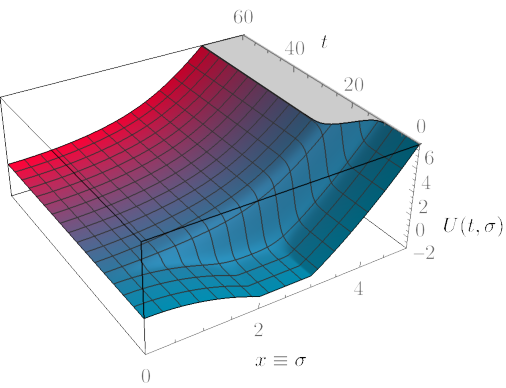
\includegraphics[width=5.5cm]{0d/figures/sc_i_on_3_n_800_xmax_10_lambda_1e6_tir_60_rg_flow_u_3d.pdf}
		\caption{Three-dimensional rendering of the flow $U(t,\sigma)$ displayed on the left \dash{} \Cref{fig:sc_i_on_3_n_800_xmax_10_lambda_1e6_tir_60_rg_flow_2d} (upper panel).}%
		\label{fig:sc_i_on_3_n_800_xmax_10_lambda_1e6_tir_60_rg_flow_u_3d}%
	}% figure/caption/label (b)
	{%
		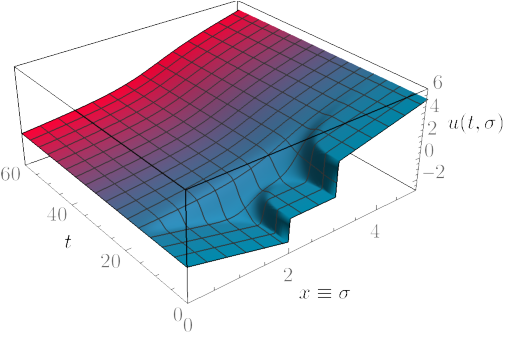
\includegraphics[width=5.5cm]{0d/figures/sc_i_on_3_n_800_xmax_10_lambda_1e6_tir_60_rg_flow_du_3d.pdf}
		\caption{Three-dimensional rendering of the flow $u(t,\sigma)$ displayed on the left \dash{} \Cref{fig:sc_i_on_3_n_800_xmax_10_lambda_1e6_tir_60_rg_flow_2d} (lower panel).}%
		\label{fig:sc_i_on_3_n_800_xmax_10_lambda_1e6_tir_60_rg_flow_du_3d}%
	}% figure/caption/label (c)
	{%
	The \frg{} flow of the effective potential $U ( t, \sigma )$ \dash{} upper panel/figure on the left~\subref{fig:sc_i_on_3_n_800_xmax_10_lambda_1e6_tir_60_rg_flow_2d} and on the right~\subref{fig:sc_i_on_3_n_800_xmax_10_lambda_1e6_tir_60_rg_flow_u_3d} \dash{} and its derivative $u ( t , \sigma ) = \partial_\sigma U ( t , \sigma )$ \dash{} lower panel/figure on the left~\subref{fig:sc_i_on_3_n_800_xmax_10_lambda_1e6_tir_60_rg_flow_2d} and on the right~\subref{fig:sc_i_on_3_n_800_xmax_10_lambda_1e6_tir_60_rg_flow_du_3d} \dash{} for the zero-dimensional $O ( 3 )$ model with initial condition \eqref{eq:testing_scenario_non-analytic_quadaratic_asymptote}. 
	The blue curves correspond to the \uv{} and the red curves to the \ir{}.
	We used the exponential regulator~\eqref{eq:exponential_regulator} with \uv{} scale $\Lambda = 10^6$.
	For the sake of readability, the plots do not show the region ${x \in[5,10]}$, because the tiny differences between $u ( t , \sigma )$ and $u ( 0 , \sigma )$ are not visible in this region and vanish for large $x = \sigma$ anyhow.
	\fromFigs{5, 6, and 7}{zerod1}%
	}% caption
	{fig:sc_i_on_3_n_800_xmax_10_lambda_1e6_tir_60_rg_flow}% label
We start our analysis with a general discussion of the \frg{} flow with \ic{} \eqref{eq:testing_scenario_non-analytic_quadaratic_asymptote}.
To this end, we fix $O(N = 3)$ to include both diffusive and advective contributions via the radial \sigmaMode{} and two pions. For $N = 3$ the number of pions is reasonably small and the (diffusive) effects of the \sigmaMode{} remain visible.
Furthermore, we choose $[ 0, x_\mathrm{max} = 10 ]$ as the spatial computational domain with $n=800$ volume cells and use the \ktScheme{} from \cref{subsec:hydroKT} for spatial discretization.
The initial cell averages $\bar{u}_i ( t = 0 )$ are computed by exact averaging\footnote{%
	Using the exact averages for $\bar{u}_i(t=0)$ has proven advantageous in terms of achievable numerical precision in the \ir{} compared to taking the mid-point values of the exact derivative of ${ \bar{u}_i ( t = 0 ) = \partial_\sigma U ( \sigma ) |_{\sigma = \sigma_i} }$ when considering non-analytic \ics{} like \cref{eq:testing_scenario_non-analytic_quadaratic_asymptote} or \eqref{eq:testing_scenario_4}.%
} 
\begin{align}
	\bar{u}_i ( t = 0 ) = \frac{1}{\Delta \sigma} \, \big[ U \big( \sigma_{i + \frac{1}{2}} \big) - U \big( \sigma_{i - \frac{1}{2}} \big) \big] ,
\end{align}
using the \uv{} \ic{} \eqref{eq:testing_scenario_non-analytic_quadaratic_asymptote}.
We use linear extrapolation \eqref{eq:BClinExt} as spatial \bc{} at $x_\mathrm{max}$ as discussed in \cref{paragraph:BCinf}.
The \uv{} scale is set to $\Lambda = 10^6$ at $t = 0$. 
Time evolution of the semi-discrete \kt{} \ode{} system is performed with \textit{NDSolve} of \WAMXIIwR{} with a \textit{PrecisionGoal} and \textit{AccuracyGoal} of 10 and stopped in the \ir{} at $r ( t_\mathrm{IR} = 60 ) \approx 10^{-20}$ using the exponential regulator shape function \eqref{eq:exponential_regulator}.
Time-stepping has not been a focus of our work and we refer the interested reader to the excellent \ccite{Ihssen:2023qaq} discussing the issue in the context of \frg{} in detail.
We find that this choice of parameters suffices to produce decent results, as discussed in the following.
There, we quantitatively analyze sources and severity of possible errors related to those (numerical) parameters.

We first provide qualitative results of our numerical methods in \cref{fig:sc_i_on_3_n_800_xmax_10_lambda_1e6_tir_60_rg_flow}, where we show the \frg{} flow of the effective potential $U ( t, \sigma )$ and its derivative $u ( t, \sigma ) = \partial_\sigma U ( t, \sigma )$ from the \uv{} (blue) to the \ir{} (red).
In the beginning, \ie{}, in the \uv{}, the system is in the broken phase. 
This changes only marginally until $t \approx 7$, which indicates that the \uv{} scale is chosen sufficiently large with $\Lambda = 10^6$.
When $r(t)$ reaches the scales of the model at $t \smallergtrsim 11$ most of the dynamics takes place (symmetry restoration) and $u ( t, \sigma )$ changes rapidly and drastically until it freezes out in the \ir{}.
In the \ir{} the system is in the restored phase as expected \apriori{}.
After $t \approx 26$ the potential does not change anymore, which indicates that one has reached a sufficiently small \ir{} scale to stop the integration.
We render this statement more precise in the following \cref{paragraph:ONRGconsistency}.
Note that the evolution in $t$ is logarithmic and corresponds to a change in scale over $25$ orders of magnitude.
At first glance this range sounds excessive, but its necessity is explained in detail in \cref{paragraph:ONRGconsistency}.

During the \frg{} evolution one observes that diffusive processes smear out the discontinuities at the non-analytic points at $\sigma = 2$ and $\sigma = 3$.
We also find that the diffusion acts in both directions \dash{} towards larger and smaller values of $\sigma$ \dash{} as expected from our discussion in \cref{subsubsec:conservative_form}. 
Nevertheless, the diffusive effects do not reach the computational boundary, which is outside the plot range at $\sigma_\mathrm{max} = 10$.
This suggests that $\sigma_\mathrm{max} = 10$ is sufficiently large.
Additionally, we observe a propagation of the conserved quantity $u$ towards smaller values of $\sigma$ via advection. 
Close to the initial discontinuities these advective processes can be interpreted as rarefaction waves. 
In a more pictorial language, the advection and diffusion ``fill up the pit'' in $u ( t, \sigma )$ at small values of $\sigma$ by moving more and more of the quantity $u$ from larger values of $\sigma$ to smaller $\sigma$ (via advection and diffusion) as well as from small negative $\sigma$ to small positive $\sigma$ (via diffusion).
Eventually the symmetry is restored and $u ( t, \sigma )$ is smoothed towards the \ir{} by diffusion. 
Furthermore, the conserved quantity $u$ does not ``pile up'' at $\sigma = 0$ after symmetry restoration, because at negative $\sigma$ exactly the opposite dynamics happens, due to the \ZII{} antisymmetry of $u ( t, \sigma )$, which is encoded in the \bc{} at $\sigma = 0$, see \cref{subsec:boundary_conditions_finite_volume}.
The differences between advective and diffusive contributions become apparent when comparing the same system for different $N$, \cf{} \cref{fig:sc_i_on_1_10_100_n_800_xmax_10_lambda_1e6_tir_60_rg_flow} and the surrounding discussion.

From a numerical perspective, the \ktScheme{} is able to handle the highly non-linear dynamics, including the non-analyticities in $u ( t, \sigma )$, without any spurious oscillatory behavior (under-/over-shooting) and allows for a stable $t$ integration to extremely small \ir{} scales.

For the sake of completeness and illustrative purposes, we also provide the \frg{} flow of the integral of $u ( t, \sigma )$, \ie{}, the effective potential $U ( t, \sigma )$, in \cref{fig:sc_i_on_3_n_800_xmax_10_lambda_1e6_tir_60_rg_flow_2d} (upper panel) and \cref{fig:sc_i_on_3_n_800_xmax_10_lambda_1e6_tir_60_rg_flow_u_3d}.
Here, the integration constant was set to zero\footnote{%
	$U ( t, 0 ) = 0$ is dictated by our choice of normalization for the zero-point function(s), see \cref{eq:normalization}.
} and the integration was performed via Riemann summation\footnote{%
	At this point we should mention that numerical results for $U ( t, \sigma )$ via Riemann summation should be treated with great caution: Numerical errors in the cell averages $\bar{u} ( t, x_j )$ which arise from the numerical \frg{} flow can accumulate during integration (here summation) along $\sigma = x$.
	More precise quadrature methods should be used if precise, quantitative values for $U ( t, \sigma )$ are needed.
} of the discrete cell averages,
	\begin{align}
		U ( t, x_i ) = \Delta x \sum_{j = 0}^{i} \frac{\bar{u} ( t, x_j )}{( 1 + \delta_{j, 0} + \delta_{j, i} )} \, .	\label{eq:riemann_sum}
	\end{align}
\Cref{fig:sc_i_on_3_n_800_xmax_10_lambda_1e6_tir_60_rg_flow_u_3d} perfectly illustrates the restoration of the $O(3)$ symmetry of the potential $U ( t, \sigma )$ during the \frg{} flow via ``vaporization'' of the infinitely many minima.
Nevertheless, we find that it is hardly possible to intuitively understand the contributions of the radial \sigmaMode{} and the pions to the \frg{} flow on the level of $U ( t, \sigma )$ only.
This complements the discussion in \cref{subsubsec:conservative_form} and lends support to our claim that the fluid-dynamical interpretation of the \frg{} flow in terms of $u ( t, \sigma )$ is superior to the canonical formulation in terms of $U ( t, \sigma )$ commonly used in the \frg{} literature.

\WarningFilter{latex}{Text page}
\fullWidthTwoColumnFigures%
	[!t] % Placement
	{%
		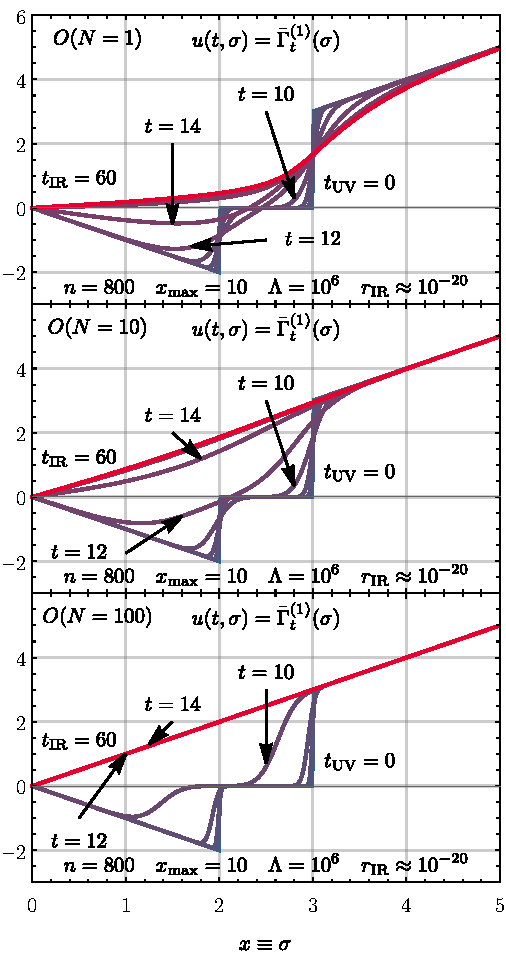
\includegraphics[width=\subcaptionFigureWidth-0.2cm]{0d/figures/sc_i_on_1_10_100_n_800_xmax_10_lambda_1e6_tir_60_rg_flow.pdf} % left figure
		\captionsetup{width=\subcaptionFigureWidth}%
		\caption{%
			The \frg{} flow of the derivative of the effective potential $u ( t , \sigma ) = \partial_\sigma U ( t, \sigma )$ for the zero-dimensional $O(N)$ model for $N = 1, \, 10, \, 100$ with \ic{} \eqref{eq:testing_scenario_non-analytic_quadaratic_asymptote}.
			All other parameters are identical to those in \cref{fig:sc_i_on_3_n_800_xmax_10_lambda_1e6_tir_60_rg_flow}.
			\fromFig{8}{zerod1}
		}
		\label{fig:sc_i_on_1_10_100_n_800_xmax_10_lambda_1e6_tir_60_rg_flow}
	}
	{\fullWidthTwoColumnFigureSpacing}
	{%
		\vspace{.065cm}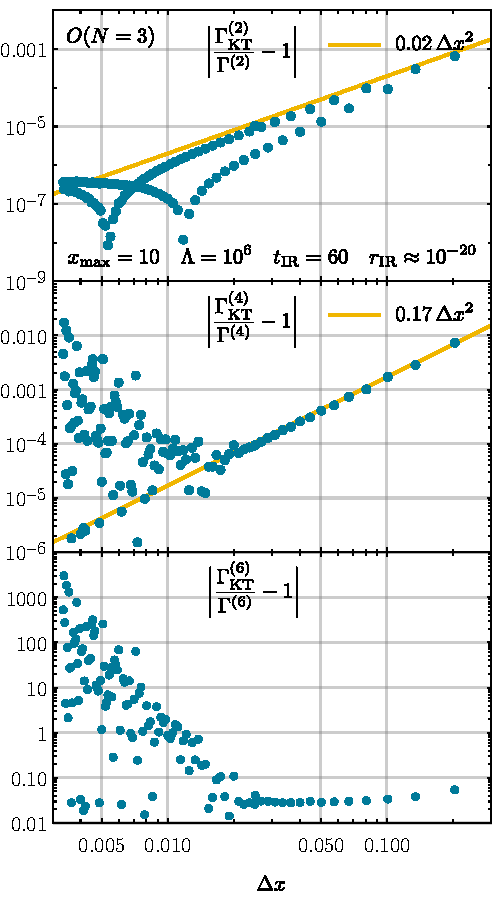
\includegraphics[width=\subcaptionFigureWidth+0.2cm]{0d/figures/sc_i_on_3_xmax_10_lambda_1e6_tir_60_deltax_scaling.pdf} % Right figure
		\captionsetup{width=\subcaptionFigureWidth}%
		\caption{%
			The relative error of the numerical results (blue dots) from the \kt{} scheme for the \ipi{} \nptFunctions{} $\Gamma^{(2n)}$ for $n = 1, 2, 3$ as a function of $\Delta x$ with \ic{} \eqref{eq:testing_scenario_non-analytic_quadaratic_asymptote}.
			The numerical derivatives at $\sigma = 0$ of $u(t_\mathrm{IR}=60, \sigma)$ were calculated via the second-order accurate central schemes \eqref{eq:derivative_1_central_error_2}, \eqref{eq:derivative_3_central_error_2}, and \eqref{eq:derivative_5_central_error_2}.
			The plot was produced with $x_\mathrm{max} = 10$, but could have been calculated for any sufficiently large $x_\mathrm{max}$.
			We used the exponential regulator~\eqref{eq:exponential_regulator} with \uv{} scale $\Lambda = 10^6$.
			The yellow straight lines $\propto \Delta x^2$ are for optical guidance.
			\fromFig{9}{zerod1}%
		}%
		\label{fig:sc_i_on_3_xmax_10_lambda_1e6_tir_60_deltax_scaling}
		\vspace{1cm}
	}%
\WarningFilter*{latex}{Text page}
Before discussing quantitative results and sources of (numerical) errors in \frg{} flows, we briefly return to the interpretation of the radial \sigmaMode{} as diffusion and the interpretation of the pions as advection in the \frg{} flow along the field space direction.
To this end, we discuss \frg{} flows for the same \uv{} initial potential \eqref{eq:testing_scenario_non-analytic_quadaratic_asymptote} as before, but for different $N$.
This  corresponds to a different number of pions in the flow and different advection velocities \eqref{eq:advection_velocity}.
All other parameters remain unchanged.
In addition to the $N = 3$ case in \cref{fig:sc_i_on_3_n_800_xmax_10_lambda_1e6_tir_60_rg_flow}, we provide the \frg{} flows of $u ( t, \sigma )$ for $N = 1, 10, 100$ in \cref{fig:sc_i_on_1_10_100_n_800_xmax_10_lambda_1e6_tir_60_rg_flow}.
The figure again demonstrates on a qualitative level that the \sigmaMode{} enters the \frg{} as diffusion, while pions enter as advection: Increasing the number of pions the problem becomes more advection-driven exhibiting more pronounced waves and faster propagation.
This can be seen by comparing the plots at equal \rgtimes{}.
For $N = 1$, the problem reduces to the pure diffusion equation \eqref{eq:pde_gamma}, where the dynamics is slowest and the diffusion propagates the fluid from negative $\sigma$ to small positive $\sigma$ close to $\sigma = 0$.
Furthermore, one observes stronger smearing of the discontinuities at $\sigma = 2$ and $\sigma = 3$.
The $N = 100$ case is extremely advection-dominated.
In the fluid-dynamical language, this corresponds to a complete suppression of diffusion, which is clearly observed from the fast propagation of the rarefaction waves and almost negligible smoothing of the discontinuities at $\sigma = 2$ and $\sigma = 3$.
We will discuss the qualitative and quantitative differences between \frg{} flows at small $N$ with flows large and even infinite $N$ in \cref{subsec:0dLargeN}.

\paragraph{Tests of the spatial resolution}\phantomsection\label{paragraph:ONdeltax}\mbox{}\\%
This paragraph is dedicated to quantifying numerical errors in the \frg{} flow arising from the finite spatial resolution $\Delta x\equiv \Delta \sigma$ of the cells in the \ktScheme{}.
Any spatial discretization comes with a discretization error.
The \ktScheme{}, which is used throughout this thesis, is formally of second-order accuracy in $\Delta x$ when employing the numerical fluxes of \cref{eq:FVKTO2} with the five-point stencil \eqref{eq:kt_stencil}.
Therefore, the numerical errors arising from the spatial discretization should scale with $\Delta x^2$ when $\Delta x$ is decreased.

As test values (observables) we use the modulus of the relative errors of the \ipi{} \nptFunctions{} $\Gamma^{(2n)}$ for $n = 1, 2, 3$,
\begin{align}
	\bigg| \frac{\Gamma^{(2n)}_\mathrm{KT}}{\Gamma^{(2n)}} - 1 \bigg| \, ,	\label{eq:relative_errors_gamma_2n}
\end{align}
where $\Gamma^{(2n)}_\mathrm{KT}$ is calculated from the \frg{} (via the \ktScheme{}) and $\Gamma^{(2n)}$ from the integral, see \cref{tab:sc_1_n_point_functions_exact}.
In order to determine how much of the relative numerical error~\eqref{eq:relative_errors_gamma_2n} is directly related to the spatial discretization, we have to optimize all other parameters of the computation in order to reduce other sources of errors.
We basically choose the same parameter set \dash{} \viz{} $\Lambda = 10^6$, $x_\mathrm{max} = 10$ and $t_\mathrm{IR} = 60$ \dash{} and \uv{} \ic{} \eqref{eq:testing_scenario_non-analytic_quadaratic_asymptote} which was also used for the qualitative analysis in the previous paragraph and only vary the number of cells $n$ to change the resolution $\Delta x$.
\WlogA{} we keep $N=3$.

Before we embark on our discussion, we remark that the spatial-discretization error enters the relative errors~\eqref{eq:relative_errors_gamma_2n} in a twofold way: 
\begin{enumerate}
	\item	There is the discretization error which comes from the \ktScheme{} during the \frg{} time integration.
	This error shows up directly in the \ir{} values $u ( t_\mathrm{IR}, x_i )$ and should scale according to $\Delta x^2$ for the chosen second-order \ktScheme{}.

	\item	There is a discretization error which is related to the extraction of the \ipi{} \nptFunctions{} from the discrete $\bar{u} ( t_\mathrm{IR}, x_i )$. 
	They have to be calculated at the physical point (the minimum at $x = \sigma = 0$) via numerical differentiation, which also comes with a discretization error.
	The latter is also related to the spatial resolution $\Delta x$.
	In general (especially in higher-dimensional models) it is not clear whether these numerical derivatives at the physical point are always well-defined.
	We argued before that $u ( t, \sigma )$ might exhibit non-analytical behavior also at the physical point in the \ir{}, \cf{}\ \ccite{Grossi:2019urj,Grossi:2021ksl,Borchardt:2016pif,Stoll:2021ori}, such that a naive numerical differentiation is not allowed in general.
	In the special case of zero-dimensional \qfts{}, we proved in \MWApp{} that the \ir{} effective action and the \ir{} potential $U ( t \rightarrow \infty, \vec{\varphi}\, )$ are smooth, which also translates to $u ( t \rightarrow \infty, \sigma )$, such that numerical differentiation (\eg{}, via finite-difference approximations) is well-defined.
\end{enumerate}
However, even though finite-difference formulas are reliable approximations for derivatives of a smooth function and have a well-defined truncation-error scaling in powers of $\Delta x$, there remains a well-known subtlety: While decreasing the resolution $\Delta x$, one eventually will reach a point where the error starts increasing again contrary to the formal truncation-error scaling. 
This is related to the ill-conditioned nature of finite-difference formulas and to explicit rounding errors in floating-point arithmetic, which increase the error of the numerical derivative below a certain $\Delta x$, see, \eg{}, Chap.~5.7 of \ccite{PresTeukVettFlan92}.
Related spurious cancellations occur if the discrete data of a smooth function include some sort of noise.
In our case this ``noise'' is directly related to the spatial-discretization errors from the \ktScheme{} and the errors from \rgtime{} integration using numerical \ode{} solvers.
These errors might be tiny, but can easily inflate the errors of the numerical derivatives, especially for higher-order derivatives.

In conclusion, while decreasing $\Delta x$, we expect that long before the relative errors from the \ktScheme{} start increasing again (because the \ktScheme{} begins operating close to machine precision or because the error of the time stepping becomes relevant) the relative errors \eqref{eq:relative_errors_gamma_2n} start increasing due to the numerical differentiation of slightly ``noisy data''. 
This phenomenon is expected to set in at larger $\Delta x$ for approximations for higher-order derivatives and long before the formal error scaling of the \ktScheme{} is no longer valid.

Our explicit results for the scaling of the relative errors with decreasing spatial resolution are presented in \cref{fig:sc_i_on_3_xmax_10_lambda_1e6_tir_60_deltax_scaling}, where we show the relative errors \eqref{eq:relative_errors_gamma_2n} for the \hbox{two-}, \hbox{four-}, and six-point functions in a double-logarithmic plot over $\Delta x$.
For $\Gamma^{(2)}$ and $\Gamma^{(4)}$ we find that the corresponding relative errors scale with $\Delta x^2$ (or even slightly better) as expected from the error scaling of the \ktScheme{} as well as the error scaling of the finite-difference stencils~\eqref{eq:derivative_1_central_error_2} and \eqref{eq:derivative_3_central_error_2}.
We observe two groups of points for $\Gamma^{(2)}$ (upper panel of \cref{fig:sc_i_on_3_xmax_10_lambda_1e6_tir_60_deltax_scaling}), which are related to discretization errors of the discontinuous \ic{} \eqref{eq:testing_scenario_non-analytic_quadaratic_asymptote} at $x=2$ and $x=3$. 
The error scaling of $0.02\, \Delta x^2$ for $\Gamma^{(2)}$ is a conservative estimate for the observed errors, which are actually lower for $\Delta x \smallergtrsim 0.005$. 
For $\Delta x \smallerlesssim 0.005$ we observe deviations from the conservative estimate for the error scaling of $\Gamma^{(2)}$ related to other error sources.
In the middle panel of \cref{fig:sc_i_on_3_xmax_10_lambda_1e6_tir_60_deltax_scaling}, we clearly see that there is an optimal minimal $\Delta x \approx 0.02$ where the correct formal scaling of the numerical derivative breaks down and the relative error of $\Gamma^{(4)}$ increases again for smaller $\Delta x$.
We can be sure that this breakdown of the error scaling is related to the numerical differentiation and not the \ktScheme{} because we observe scaling with at least $\Delta x^2$ for $\Gamma^{(2)}$ in the upper panel of \cref{fig:sc_i_on_3_xmax_10_lambda_1e6_tir_60_deltax_scaling} well below $\Delta x \approx 0.02$.
This is expected for lower-order numerical derivatives.
Furthermore, we find that for $\Gamma^{(6)}$ (lower panel of \cref{fig:sc_i_on_3_xmax_10_lambda_1e6_tir_60_deltax_scaling}) the order of the numerical derivative is already too large, such that the theoretical error scaling of the \ktScheme{} cannot be seen at all and is completely obscured by the errors from the numerical differentiation of $\bar{u} ( t_\mathrm{IR}, x_i )$.

We conclude that the \ktScheme{} is perfectly suited for the spatial discretization of the \frg{} flow equation for $u ( t, \sigma )$ and shows correct scaling with decreasing spatial resolution $\Delta x$. 
This is also confirmed by tests with different \ics{}, see, \eg{}, \cref{fig:sc_ii_n_on_4_xmax_10_lambda_1e12_tir_60_deltax_scaling}.

In addition, we actually found that a more severe problem is the correct extraction of physical observables from the \ir{} values $\bar{u} ( t_\mathrm{IR}, x_i )$, which are usually related to derivatives of $u ( t_\mathrm{IR}, \sigma )$.
We predict that this problem might even become more severe in higher dimensions, were the \ir{} potential is no longer guaranteed to be smooth.
We therefore suggest to search for better ways of calculating those derivatives as well as for careful analysis tools for numerically calculated \ipi{} \nptFunctions{} in the vicinity of non-analyticities in general.
However, this is beyond the scope of the present work.

We remark that our numerical findings indicate that \dash{} independent of the specific numerical discretization scheme \dash{} the number of grid points or expansion coefficients might have been chosen too small in previous \frg{} studies in literature to obtain a decent resolution.
However, other works, \cf{} \ccite{Pelaez:2015nsa,Caillol:2012zz,Pangon:2009pj,Pangon:2010uf,Borchardt:2015rxa,Borchardt:2016pif}, which also discuss the limitations of their numerical schemes in detail, have used a rather large number of discretization points \dash{} in some cases to compensate the demand for continuity of the specific schemes.

In the following we will mostly use a spatial resolution of 
	\begin{align}
		\Delta x = \frac{x_\mathrm{max}}{n - 1} \simeq 0.025 \, ,
	\end{align}
where we can trust the results for the two- and four-point functions.
The relative errors for the six-point function will only be plotted for the sake of completeness, but cannot be included in any reasonable quantitative analysis of other sources of (numerical) errors in \frg{} flow equations although they are still at a reasonably small level of $\sim 5\%$ at $\Delta x \simeq 0.025$.

\paragraph{Tests of the size of the computational domain}\phantomsection\label{paragraph:test_size_computational_domain}\mbox{}\\%
\fullWidthTwoColumnSubFigures%
	[!t]% Placement
	{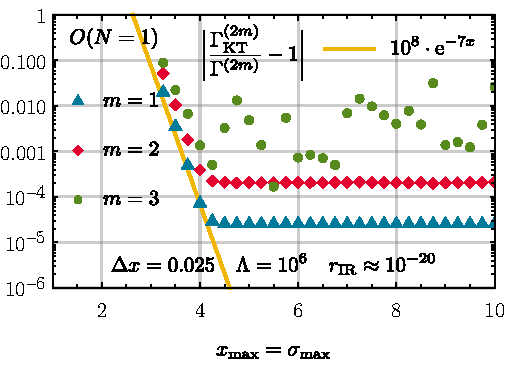
\includegraphics[width=\subcaptionFigureWidth]{0d/figures/sc_i_on_1_deltax_25e-3_lambda_1e6_tir_60_errors_xmax.pdf}}% Left figure (dummy index a)
	{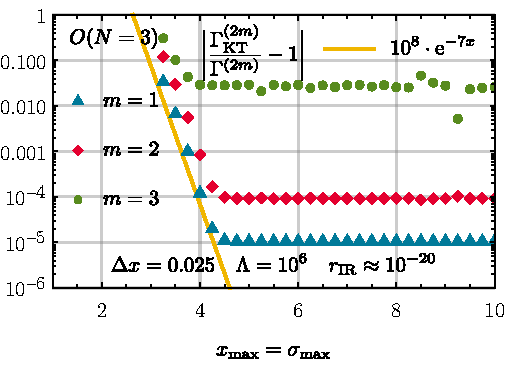
\includegraphics[width=\subcaptionFigureWidth]{0d/figures/sc_i_on_3_deltax_25e-3_lambda_1e6_tir_60_errors_xmax.pdf}}% Right figure (dummy index b)
	[fig:sc_i_on_1_deltax_25e-3_lambda_1e6_tir_60_errors_xmax,fig:sc_i_on_3_deltax_25e-3_lambda_1e6_tir_60_errors_xmax] %Labels
	{%
		The relative error for $\Gamma^{(2m)}$ for $m = 1, 2, 3$ for the \uv{} potential \eqref{eq:testing_scenario_non-analytic_quadaratic_asymptote} of the \ONn{1} model on the left \subref{fig:sc_i_on_1_deltax_25e-3_lambda_1e6_tir_60_errors_xmax} and of the \ONn{3} model on the right \subref{fig:sc_i_on_3_deltax_25e-3_lambda_1e6_tir_60_errors_xmax} as a function of $x_\mathrm{max}$, while keeping the cell size constant, $\Delta x = 0.025$. $\Gamma^{(2m)}$ are computed from the discrete values of the derivative of the \ir{} potential $u ( t_\mathrm{IR} = 60, \sigma )$ via the second-order accurate central finite-difference stencils~\eqref{eq:derivative_1_central_error_2}, \eqref{eq:derivative_3_central_error_2}, and \eqref{eq:derivative_5_central_error_2} at $\sigma = 0$.
		We use the exponential regulator~\eqref{eq:exponential_regulator} with \uv{} scale $\Lambda = 10^6$.
		The yellow straight line $\propto\exp{-7x_\mathrm{max}}$ is for optical guidance.
		\fromFigs{10 and 11}{zerod1}%
	}% Caption
	{fig:sc_i_on_deltax_25e-3_lambda_1e6_tir_60_errors_xmax}% Label
In this paragraph, we discuss the influence of the size of the computational domain $[ 0, \sigma_\mathrm{max} ]$ on the relative errors of the \ir{} observables \eqref{eq:relative_errors_gamma_2n}.
As discussed in \cref{subsec:boundary_conditions_finite_volume}, we expect that, if the spatial \bcs{} are not implemented with great caution and the computational domain is too small, one cannot trust the results from the numerical integration of the \frg{} flow.
If the computational domain is too small, we expect large errors, because the \bcs{} at $\sigma_\mathrm{max}$ are no longer valid due to wrong extrapolation to the ghost cells and consequently wrongly estimated influx.

In the case with \uv{} \ic{} \eqref{eq:testing_scenario_non-analytic_quadaratic_asymptote}, the \bc{} at $\sigma_\mathrm{max}$ is implemented as a linear extrapolation \eqref{eq:BClinExt} of $u ( t, \sigma )$ to the two ghost cells of the \ktScheme{} to mimic the asymptotic behavior of $u ( t, \sigma )$. 
As long as $\sigma_\mathrm{max}$ is sufficiently large, we expect only tiny deviations of $u ( t, \sigma )$ from its initial \uv{} value $u ( t_\mathrm{UV} = 0, \sigma )$ around $\sigma_\mathrm{max}$.
However, if $\sigma_\mathrm{max}$ is too small and approaches the model scales, we expect the diffusive effects to reach the boundary of the computational domain, such that a linear extrapolation is no longer a good approximation in order to determine the spatial \bc{}.

To this end, we test the scaling of the relative errors \eqref{eq:relative_errors_gamma_2n} with decreasing computational domain size $x_\mathrm{max} = \sigma_\mathrm{max}$ for $N = 1$ (purely diffusive) and $N = 3$. 
The results and (numerical) parameters are shown in \cref{fig:sc_i_on_deltax_25e-3_lambda_1e6_tir_60_errors_xmax}.
In both cases ($N=1$ and $N=3$ in \cref{fig:sc_i_on_1_deltax_25e-3_lambda_1e6_tir_60_errors_xmax,fig:sc_i_on_3_deltax_25e-3_lambda_1e6_tir_60_errors_xmax} respectively) we find that the relative errors are independent of $\sigma_\mathrm{max}$ for sufficiently large $\sigma_\mathrm{max}$.
However, if the spatial cutoff $\sigma_\mathrm{max}$ is approaching the model scales (here the discontinuity in $u ( t_\mathrm{UV} = 0, \sigma )$ at $\sigma = 3$, see \cref{fig:sc_i_uv_initial_condition}) the relative errors for $\Gamma^{(2)}$ and $\Gamma^{(4)}$ start rising exponentially.

Contrary to our expectations, the results for $N = 1$ and $N = 3$ are very similar and the exponential rise of the relative errors sets in at a similar $\sigma_\mathrm{max}\approx 4.2$.
\Apriori{} we expected that for the purely diffusive scenario with $N = 1$, the diffusive effects arising from the large gradients at $\sigma = 3$ might have more time to reach and influence the shape of $u ( t, \sigma )$ at larger values of $\sigma$, which does not seem to be the case.
Our employed monitors for numerical errors \dash{} the \ipi{} \nptFunctions{} in the \ir{} computed at $\sigma=0$ and $t=0$ \dash{} are rather intensive to such changes.
A possible explanation is the fact that observable errors from the boundary at $\sigma_\mathrm{max}$ propagate into the computational domain at a finite speed\footnote{
	In the context of ``infinite propagation speeds'' in parabolic \pdes{}, \cf{} the discussion and corresponding footnote~\ref{footnote:HEinf} in \cref{subsec:hydroDiffusion}, we refer here to the fact that observable changes on the relevant scales of the problem travel with apparently finite speed independent from some formal instantaneous, infinitesimal (exponentially decaying) changes.% 
}, which is rather low in the purely diffusive case and in general small at large~$\sigma$, and thus do not influence the physical point at $t=0$ and $\sigma=0$. 

Nevertheless, we conclude from \cref{fig:sc_i_on_1_deltax_25e-3_lambda_1e6_tir_60_errors_xmax,fig:sc_i_on_3_deltax_25e-3_lambda_1e6_tir_60_errors_xmax} that it is extremely important to use sufficiently large computational domains to minimize numerical errors in field-dependent \frg{} flows. 
This implies that $\sigma_\mathrm{max}$ should be chosen much larger than all relevant scales of the model.

\fullWidthTwoColumnSubFigures
	[!t] % Placement
	{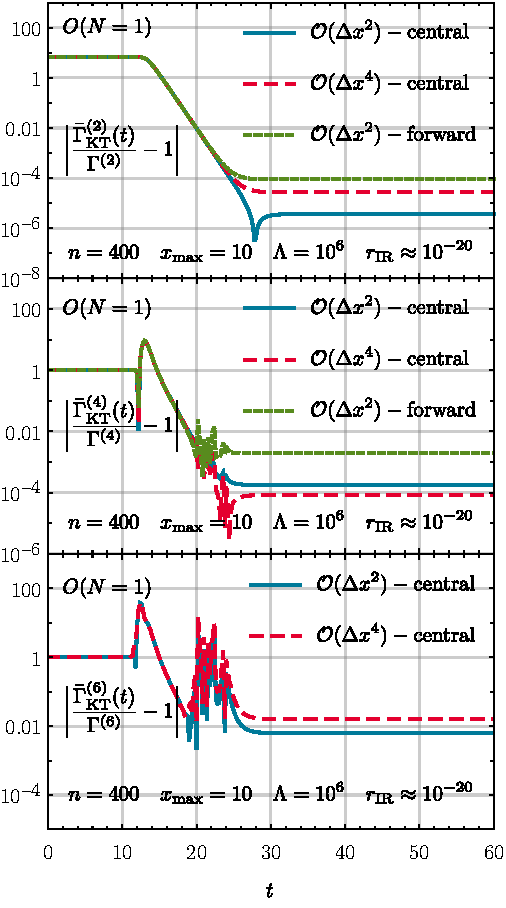
\includegraphics[width=\subcaptionFigureWidth]{0d/figures/sc_i_on_1_n_400_xmax_10_lambda_1e6_tir_60_flow_errors.pdf}} % left figure (dummy index a)
	{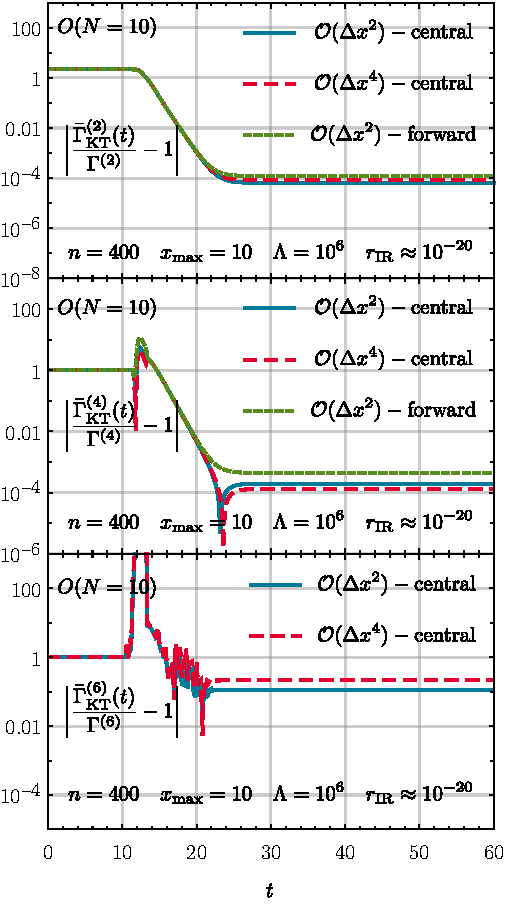
\includegraphics[width=\subcaptionFigureWidth]{0d/figures/sc_i_on_10_n_400_xmax_10_lambda_1e6_tir_60_flow_errors.pdf}} % Right figure (dummy index b)
	[fig:sc_i_on_1_n_400_xmax_10_lambda_1e6_tir_60_flow_errors,fig:sc_i_on_10_n_400_xmax_10_lambda_1e6_tir_60_flow_errors] %Labels
	{%
		The relative error for $\Gamma^{(2m)}$, for $m = 1, 2, 3$, calculated with the \kt{} scheme as a function of the \rgtime{} $t$ for the \ONn{1} model on the left~\subref{fig:sc_i_on_1_n_400_xmax_10_lambda_1e6_tir_60_flow_errors} and of the \ONn{10} model on the right~\subref{fig:sc_i_on_10_n_400_xmax_10_lambda_1e6_tir_60_flow_errors}.
		The \uv{} initial potential is given by \cref{eq:testing_scenario_non-analytic_quadaratic_asymptote}. 
		We use the exponential regulator~\eqref{eq:exponential_regulator} with \uv{} scale $\Lambda = 10^6$. 
		The computational grid has $n=400$ cells and $\sigma_\mathrm{max} = x_\mathrm{max} = 10$. $\Gamma^{(2m)}$ are extracted from $u ( t_\mathrm{IR} = 60, \sigma )$ via the finite-difference stencils \eqref{eq:derivative_1_central_error_2}\dash{}\eqref{eq:derivative_5_central_error_4}.
		\fromFigs{13 and 15}{zerod1}
	} % Caption
	{fig:sc_i_on_n_400_xmax_10_lambda_1e6_tir_60_flow_errors} % Label
From our findings, it is therefore expected that choosing a large $\sigma_\mathrm{max}$ might even gain in importance in higher-dimensional models, where the physical point may be located at a non-trivial minimum in the \ir{}, like in the \qm{} and \gnyBm{} of \cref{chap:GN,chap:QMM}. 
If the physical point is closer to the boundary of the computational domain the relative errors for observables might even be larger than for our zero-dimensional model where the physical point moves towards $\sigma = 0$ during the \frg{} flow. 
In terms of errors originating from the boundary at $\sigma_\mathrm{max}$, the physical point at $\sigma = 0$ is ideal since it has the largest spatial and \dash{} in a sense causal, due to the finite speed of propagation \dash{} distance to $\sigma_\mathrm{max}$.

Lastly, we have to warn that there is no panacea for the construction of a sufficiently large computational domain and the choice of $\sigma_\mathrm{max}$ has to be adjusted to the specific model and specific \ic{} under consideration. 
For some problems even more involved approaches (like using several computational grids of different resolution $\Delta x$) might be needed or are at least highly advantageous~\cite{Grossi:2019urj,Grossi:2021ksl,Ihssen:2022xkr,Ihssen:2023xlp}.
In any case one has to check that the \ir{} results do not depend on the size of the computational domain (even if exact reference values for observables are unknown), \cf{} \ccite{Pangon:2009pj,Caillol:2012zz,Stoll:2021ori}.
This can be done by fixing appropriate values for the spatial resolution $\Delta x$ as well as for all other (numerical) parameters and successively increasing $\sigma_\mathrm{max}$ until the \ir{} observables do not change anymore.

\paragraph{Tests of the \uv{} and \ir{} scales}\phantomsection\label{paragraph:ONRGconsistency}\mbox{}\\%
We now turn to a long-standing discussion in the \frg{} community, namely the question: How do we have to choose the initial \uv{} and numerical \ir{} cutoff scale for the calculation of the 
\frg{} flow for a specific model? 

A common argument is based on the energy scales of a given model. The \uv{} \ic{} is fixed at \uv{} scales $\Lambda$ that are close to the largest energy scale of the model.
Higher $\Lambda$ are excluded by arguing that at higher energy scales other physical degrees of freedom (\eg{}, other interaction channels or new particles) are relevant and the model at hand is only valid within a certain energy regime.
On the other hand, the \ir{} cutoff $k_\mathrm{IR}$ scale is oftentimes fixed by arguing that if it decreases below the lowest energy scale of the model, the \frg{} flow is effectively ``frozen in'' and the effective potential no longer changes anyway.
A relatively low \uv{} initial scale and a high \ir{} cutoff lead to rather short flow times of only $t_\mathrm{UV} - t_\mathrm{IR} \approx 3 - 4$.

Another approach, which is sometimes employed in conjunction with the first strategy, is guided by the principle of ``numerical stability'' of the \frg{} flow, where cutoffs are chosen in a certain way to ``improve performance and stability'' during the numerical \rgtime{} integration.
In turn, in \ccite{Pelaez:2015nsa,Caillol:2012zz,Pangon:2009pj,Pangon:2010uf,Borchardt:2016pif} relatively small \ir{} cutoff scales are reached due to the use of numerical stable schemes or the control of stability.
Careful extrapolations into the deep \ir{} like the ones discussed in, \eg{}, \ccite{Pelaez:2015nsa,Grossi:2019urj,Grossi:2021ksl} are another possibility to achieve low \ir{} cutoffs.
Note that, for theories in $d>0$ dimensions, numerical integration into the (deep) \ir{} becomes very demanding due to multiple reasons, see also \ccite{Pelaez:2015nsa,Grossi:2019urj,Grossi:2021ksl,Stoll:2021ori} and especially \ccite{Ihssen:2023qaq}.
This is probably the main reason why often large numerical \ir{} cutoffs are used.

In general, however, there is a well-defined strategy for the choice of the \uv{} scale scale: the notion of \textit{renormalization group consistency} introduced in \cref{subsec:RGconsistency}.
Recalling the central statement of \cref{eq:rgcCondition}: 
\begin{align}
	\Lambda\dod{\Gamma[\vec{\varphi}\vts]}{\Lambda}\equiv \Lambda\dod{\FSeaa_0[\vec{\varphi}\vts]}{\Lambda}\overset{!}{=} 0\,,\label{eq:rgcConditionONd0}
\end{align}
\ie{}, the full effective action $\Gamma [\vec{\varphi}\vts]$ in the \ir{} must be independent of the \uv{} initial scale~\cite{Braun:2018svj}.
In the context of \frg{} as an integral deformation in zero dimensions, see \cref{subsec:0dintegrals}, the \uv{} scale scale $\Lambda$ has to be much larger than all scales in the model.
Hence our zero-dimensional models fall in the scenario discussed with \cref{eq:rgcScales} in the first paragraph of \cref{subsubsec:rgcICS}.
In this sense, a high \uv{} initial scale is necessary to include all fluctuations \dash{} to guarantee \cref{eq:rgcScales}.
It was already demonstrated in \ccite{Braun:2018svj} that if the \uv{} initial scale $\Lambda$ is chosen too small and too close to the model scales or external scales, physical results are spoiled drastically by slightly varying $\Lambda$ and \cref{eq:rgcConditionONd0} is not fulfilled anymore, \cf{} \nbccite{Braun:2003ii,Herbst:2013ufa,Springer2017,PhysRevD.87.076004} for related discussions in the context of \loefts{} of \qcd{} and also \cref{chap:GN,chap:QMM} for further discussions of \rgcy{} in the context of this thesis.

A hard lower limit for $\Lambda$ arises from the fact that for a given \ic{} $U(t=0,\sigma)$
\begin{subequations}\label{eq:LambdaMin}
\begin{align}
	\Lambda + \tfrac{1}{\sigma} \, \partial_\sigma U( t = 0, \sigma ) > \, & 0 \, ,	\label{eq:LambdaMin1}\\*[.1em] % no pagebreak
	\Lambda + \partial_\sigma^2 U( t = 0, \sigma ) > \, & 0 \, ,\label{eq:LambdaMin2}
\end{align}
\end{subequations}
must hold $\forall\sigma$ to have a non-singular flow equation~\eqref{eq:conservation_law_u_phi}. 
This is discussed, \eg{}, in Refs.~\cite{Pelaez:2015nsa,Schaefer:2001cn} and represents a minimal requirement for $\Lambda$ when considering a given \ic{} $U(t=0,\sigma)$.
However, guaranteeing the inequalities \eqref{eq:LambdaMin} does by itself \apriori{} not guarantee \rgcy{} in the sense of \cref{eq:rgcConditionONd0}.

For higher-dimensional \qfts{} it is actually complicated to quantify the relative error of observables from violations of \cref{eq:rgcConditionONd0}, because ``exact'' reference values, \eg{}, by numerical calculation of expectation values from the functional integral, are rarely known, especially for \loefts{}.
In zero-dimensional \qft{} this is different, because we can directly calculate the relative errors for observables like \ipi{} \nptFunctions{}, \cf{} \cref{eq:relative_errors_gamma_2n}, for different values of $\Lambda$.

Similar arguments apply to the \ir{} cutoff, where the numerical integration of the \frg{} flow is stopped.
Here, one must clearly state that the full effective average action $\Gamma [ \chi ]$ in the \ir{} is unambiguously defined via the limit ${t \rightarrow \infty \leftrightarrow r(t) \rightarrow 0}$ of $\bar{\Gamma}_t [ \chi ]$, \cf{}\ \cref{eq:scale_dependent_effective_average_action}.
In practice, a direct integration to $t \rightarrow \infty$ is numerically impossible, which implies that one has at least to make sure that the numerical \rgtime{} integration is stopped no earlier than when all observables of interest do not change anymore, or one has to systematically extrapolate to $t \rightarrow \infty$, see, \eg{}, \ccite{Grossi:2019urj,Grossi:2021ksl}.
It is worth mentioning that, depending on the specific observable, these ``freeze-out scales'' can be extremely different, see \cref{fig:sc_i_on_3_n_400_xmax_10_lambda_1e6_tir_60_mass_minimum}.\bigskip

In the following, we will therefore explicitly explore the influence of \uv{}  and \ir{} cutoff scales on the relative errors \eqref{eq:relative_errors_gamma_2n} for the $\Gamma^{(2n)}$.
We start our discussion by providing results for the relative errors \eqref{eq:relative_errors_gamma_2n} depending on the \rgtime{} $t$ for different $N$ of $O(N)$ and \uv{} \ic{} \eqref{eq:testing_scenario_non-analytic_quadaratic_asymptote}.
In \cref{fig:sc_i_on_n_400_xmax_10_lambda_1e6_tir_60_flow_errors} we plot the relative errors of $\Gamma^{(2n)}$ for $n\in\{ 1, 2, 3\}$ for $N \in\{1, 10\}$, which are all extracted via various finite-difference stencils from $u ( t, \sigma )$ at the physical point $\sigma = 0$ and different $t$ during the \frg{} flow.
A corresponding plot for $N=3$ can be found in Fig. 14 of \nbccite{zerod1}.
All (numerical) parameters are mentioned in the figures or the respective captions.

\fullWidthTwoColumnFigures%
	[!t] % Placement
	{%
		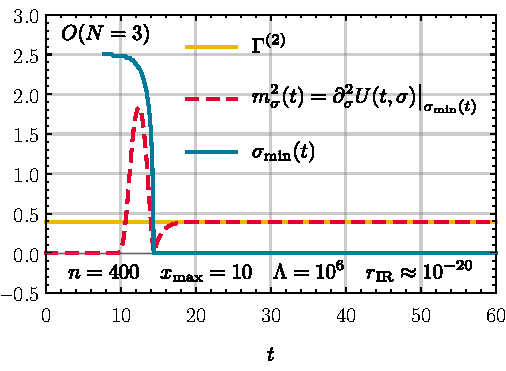
\includegraphics[width=\subcaptionFigureWidth]{0d/figures/sc_i_on_3_n_400_xmax_10_lambda_1e6_tir_60_mass_minimum.pdf} % left figure
		\captionsetup{width=\subcaptionFigureWidth}%
		\caption{%
			The \frg{} flow of the minimum $\sigma_\mathrm{min} ( t )$ ({blue}) of the effective potential $U ( t, \sigma )$ and of the curvature mass $m_\sigma^2 ( t )$ of the \sigmaMode{} ({red-dashed}) evaluated on the equations of motion~\eqref{eq:definition_j_t}, \ie{}, at the flowing minimum.
			The {blue} curve sets in after a unique minimum at $\pm \sigma_\mathrm{min} ( t )$ has formed.
			As \uv{} \ic{} we use \cref{eq:testing_scenario_non-analytic_quadaratic_asymptote}. 
			We used the exponential regulator~\eqref{eq:exponential_regulator} with \uv{} scale $\Lambda = 10^6$.
			The curvature mass $m_\sigma^2 ( t )$ was extracted from $u ( t, \sigma )$ via \cref{eq:derivative_1_forward_error_2} at the moving $\sigma_\mathrm{min} ( t )$.
			The horizontal ({yellow}) line denotes the exact \ir{} result $\Gamma^{(2)}\simeq 0.397$ at $\sigma = 0$, which must agree with $m_\sigma^2$ in the \ir{}, where $\sigma_\mathrm{min} ( t ) = 0$.
			\fromFig{12}{zerod1}%
		}%
		\label{fig:sc_i_on_3_n_400_xmax_10_lambda_1e6_tir_60_mass_minimum}%
	}%
	{\fullWidthTwoColumnFigureSpacing}%
	{%
		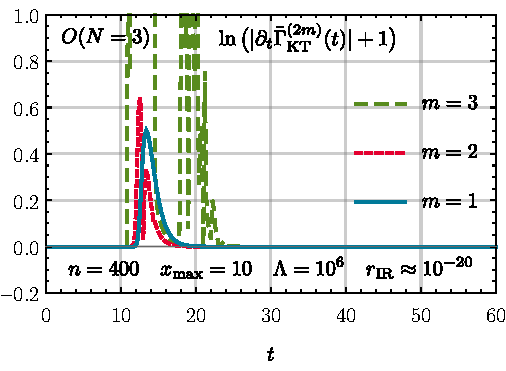
\includegraphics[width=\subcaptionFigureWidth]{0d/figures/sc_i_on_3_n_400_xmax_10_lambda_1e6_tir_60_changing_rates.pdf} % Right figure
		\captionsetup{width=\subcaptionFigureWidth}%
		\caption{
			The rate of change in $t$ of $\bar{\Gamma}^{(2m)} ( t )$ at the \ir{} minimum $\sigma = 0$ for $n = 1, 2, 3$ during the \frg{} flow.
			This rate of change is defined as the numerical \rgtime{} derivative $\partial_t \bar{\Gamma}^{(2m)} ( t )$ over the \rgtime{}.
			$\partial_t \bar{\Gamma}^{(2m)} ( t )$ are calculated via a finite-difference approximation ${[\bar{\Gamma}^{(2m)} (t) - \bar{\Gamma}^{(2m)} (t - \Delta t) ]/\Delta t}$, where $\Delta t = 0.2$.
			$\bar{\Gamma}^{(2m)} ( t )$ are obtained via numerical derivatives \eqref{eq:derivative_1_central_error_2}, \eqref{eq:derivative_3_central_error_2}, and \eqref{eq:derivative_5_central_error_2} of $u (t, \sigma)$ at $x = \sigma = 0$.
			For convenience, we added 1 and took the logarithm to highlight the regions with high rates of change of the observables $\bar{\Gamma}^{(2m)}(t)$ and to identify the freeze-out plateau, where these rates vanish.
			We used the exponential regulator~\eqref{eq:exponential_regulator} with \uv{} scale $\Lambda = 10^6$.
			\fromFig{17}{zerod1}%
		}
		\label{fig:sc_i_on_3_n_400_xmax_10_lambda_1e6_tir_60_changing_rates}
	}
In \cref{fig:sc_i_on_n_400_xmax_10_lambda_1e6_tir_60_flow_errors} (\ie{}, for $N = 1$ and $10$) and independent of the choice of discretization of the numerical derivatives, we observe plateaus for the relative errors for $\Gamma^{(2n)}$ at the beginning and the end of the \frg{} time evolution.
The plateau at small $t$ corresponds to the \uv{} regime and indicates that the \uv{} scale is chosen sufficiently large because no fluctuations are present at the \ir{} physical point until $r(t)$ reaches the scales of the model.
\rgcy{} \eqref{eq:rgcConditionONd0}, hence \uv{}-scale-independence should therefore be fulfilled, as long as we initialize our \frg{} flow at some \rgscale{} which is at the far left of this plateau.
Such a plateau at small $t$ is a sufficient condition for \rgcy{} but not a necessary one, because quantum fluctuations could already work at positions in field space away from the \ir{} physical point and only influence higher-order correlation functions.
We will quantify this in the following.
In the plots various finite-difference stencils with distinct error scaling in $\Delta x$ are used to demonstrate that the plateaus are independent of other sources of errors, like spatial discretization errors\footnote{%
	Incidentally, \cref{fig:sc_i_on_n_400_xmax_10_lambda_1e6_tir_60_flow_errors} also underlines our statement that the spatial discretization errors stemming from the numerical differentiation of $u ( t, \sigma )$ are much more severe than the discretization errors of the \ktScheme{}.
	Otherwise, the curves for the various finite-difference stencils would coincide in the \ir{}.%
}.

For intermediate $t$, we observe strong dynamics and rapid changes in the relative errors for the $\Gamma^{(2n)}$.
The actual values of the relative errors for intermediate $t$ are irrelevant for the current discussion on \uv{} and \ir{} scales.

The plateau at late \rgtimes{} $t$ corresponds to the \ir{} scale of the theory and indicates that the physical observables are frozen and do not change anymore, such that the numerical time integration can be stopped.
As expected, we find that the explicit \ir{} scale strongly depends on the choice of $N$, thus the number of pions and the related strength of advection.
The smaller $N$ and the more diffusive the system, the longer it takes to reach the \ir{}\footnote{%
	This is a well-known observation from all kinds of fluid-dynamical systems.
	It typically takes much longer to reach thermal equilibrium via diffusion alone than when including advective processes.
}: For $N = 10$ the freeze-out already sets in at $t \approx 26$, while for $N = 1$ one has to wait until $t \approx 30$ to find that the dynamics ends.
This is a difference of two orders of magnitude in the \rgscale{}.
In general, our toy model tests indicate that rather small \ir{} scales are needed to actually reach the regime where the observables are frozen. 
Still, for $N = 10$, $r(t \approx 26) \approx 5 \cdot 10^{-6}$, \ie{}, the \ir{} regime begins six orders of magnitude below the model scales.

This observation might also partially translate to higher-dimensional models, meaning that commonly used \ir{} cutoffs might be systematically chosen too large, such that predictive power is lost. Nevertheless, we expect this problem to be the less severe the higher the space-time dimensionality of a model under consideration, because of the larger phase-space (momentum suppression).
The smaller the space-time dimension of a model, the more important are long-range interactions \dash{} quantum fluctuations at small \rgscales{} $k$ \dash{} for the macroscopic observables, which is of course most extreme for $d = 0$.

Furthermore, we observe from \cref{fig:sc_i_on_3_n_400_xmax_10_lambda_1e6_tir_60_mass_minimum} as well as \cref{fig:sc_i_on_n_400_xmax_10_lambda_1e6_tir_60_flow_errors} that the freeze-out scale is slightly different for different observables, because higher \ipi{} \nptFunctions{} seem to be more sensitive to tiny changes in $u ( t, \sigma )$.
In particular, we observe from \cref{fig:sc_i_on_3_n_400_xmax_10_lambda_1e6_tir_60_mass_minimum} that the minimum $\sigma_\mathrm{min}$ is already frozen at $t \approx 14$, while the curvature mass $m_\sigma^2$ still changes drastically after $t \approx 14$ over several orders of magnitude in \rgscale{}.
This is especially interesting for higher-dimensional models: Oftentimes the freeze-out of the minimum is considered a suitable \ir{} scale to stop the \frg{} flow, which is definitely not justified, since the derivatives of the potential \dash{} the curvature mass \dash{} at the physical point are usually still changing.
Using the changing rates of the curvature mass instead of the position of the minimum as a monitor for the dynamic range \dash{} viable numerical \ir{} cutoffs \dash{} has proven crucial in the \frg{} study~\cite{Stoll:2021ori} of the \gnym{} in \cref{sec:gnyFiniteN}.

\halfWidthFigure%
	{0d/figures/sc_i_on_3_n_400_xmax_10_rir_10e-20_cutoff_test.pdf}
	[]
	{%
		The relative error for $\Gamma^{(2m)}$ for $m = 1, 2, 3$ from the \kt{} scheme as a function of the \uv{} scale scale $\Lambda$ for the initial potential \eqref{eq:testing_scenario_non-analytic_quadaratic_asymptote}.
		We use the exponential regulator~\eqref{eq:exponential_regulator} and keep the \ir{} cutoff scale constant at $r ( t_\mathrm{IR} ) = 10^{-20}$.
		Furthermore, for all data points the computational grid size is fixed at $\sigma_\mathrm{max} = x_\mathrm{max} = 10$ and the number of volume cells is set to $n = 400$.
		$\Gamma^{(2m)}$ are calculated from $u ( t_\mathrm{IR} = 60, \sigma )$ via the approximations \eqref{eq:derivative_1_central_error_2}, \eqref{eq:derivative_3_central_error_2}, and \eqref{eq:derivative_5_central_error_2} for the numerical derivatives. The yellow straight line $\propto\Lambda^{-1}$ is for optical guidance.
		\fromFig{16}{zerod1}
	}%
	{fig:sc_i_on_3_n_400_xmax_10_rir_10e-20_cutoff_test}
Next, we explicitly quantify the relative errors of $\Gamma^{(2n)}$, which stem from too small \uv{} scales $\Lambda$ and the violation of \rgcy{} \eqref{eq:rgcConditionONd0}.
To this end, we plot the relative errors \eqref{eq:relative_errors_gamma_2n} as a function of the \uv{} scale $\Lambda$, while keeping the \ir{} cutoff scale fixed at extremely small $r ( t_\mathrm{IR}) = 10^{-20}$.
In \cref{fig:sc_i_on_3_n_400_xmax_10_rir_10e-20_cutoff_test} we observe that the \ir{} observables become independent of $\Lambda$ at rather large $\Lambda \approx 10^6$.
This is several orders of magnitude above the model scales, contrary to what is often used in \frg{} studies in higher dimensions.
If the \uv{} scale is chosen too small, we find that the relative errors of $\Gamma^{(2n)}$ grow proportional to $\frac{1}{\Lambda}$, as estimated in \cref{eq:error_scaling_uv_cutoff}.
Surprisingly, it turns out that the \rgcy{} condition \eqref{eq:rgcConditionONd0} is already violated at rather large \uv{} scale scales $\Lambda \approx 10^5$ and is only fulfilled for $\Lambda \smallergtrsim 10^5$. 
We conclude that great care is required when specifying the \uv{} scale in a \frg{} calculation.

Before we close this discussion, we provide a natural measure to estimate the correct \uv{} and \ir{} scales of a model or theory, even if there are no exact reference values for observables that can be used for comparison with the \frg{} results.
To this end, we plot in \cref{fig:sc_i_on_3_n_400_xmax_10_lambda_1e6_tir_60_changing_rates} the shifted logarithm of the changing rates of the $\bar{\Gamma}^{(2n)} ( t )$ at the \ir{} minimum $\sigma = 0$ over \rgtime{} $t$.
These quantities have to vanish in the \uv{} and the \ir{}, when the relative errors \eqref{eq:relative_errors_gamma_2n} are not changing.

A similar investigation can be done for any other model or theory and can be used as an indication to ensure sufficiently large \uv{} and sufficiently small \ir{} cutoffs: A first estimate may be obtained by choosing $\Lambda$ and $t_\mathrm{IR}$ in a way that the plateaus (or scaling regimes) in figures similar to \cref{fig:sc_i_on_3_n_400_xmax_10_lambda_1e6_tir_60_changing_rates} are of approximately equal \rgtime{} duration than the time interval in which the actual dynamics takes place. 
In the absence of an explicit and accessible error estimate, rates of change are a cheap and simple tool to study the \uv{} and \ir{} limits of \rgtime{} evolution, \cf{} \cref{subsec:gnyFiniteNresults}.
\FloatBarrier
\subsubsection{Test case II: \texorpdfstring{$\phi^4$}{phi**4} theory}
\label{subsubsec:sc2}
The \textit{test case II} is a zero-dimensional version of $\phi^4$ theory with the \uv{} initial potential
	\begin{align}
		U ( \vec{\varphi} \vts ) = \mp \tfrac{1}{2} \, \vec{\varphi}^{\vts 2} + \tfrac{1}{4!} \, ( \vec{\varphi}^{\vts 2} )^2 \, ,	\label{eq:testing_scenario_phi4}
	\end{align}
where a theory with negative mass term $-\tfrac{1}{2} \, \vec{\varphi}^{\vts 2}$ has a \textit{``sombrero''}-type (symmetric double-well) potential well-known from standard textbook discussions of spontaneous symmetry breaking~\cite{Goldstone:1961eq,Goldstone:1962es}.
The corresponding \ic{} with negative mass term for the \frg{} flow is illustrated in \cref{fig:sc_ii_n_uv_initial_condition}.
When not explicitly stated otherwise we will consider the \ic{} \eqref{eq:testing_scenario_phi4} with negative mass term.
The reference values for the exact \ir{} \ipi{} vertex functions $\Gamma^{(2n)}$ of the $O(N)$ model \eqref{eq:on-model_relation_2pf_phi2}\nolinebreak[3]--\nolinebreak[2]\eqref{eq:on-model_relation_6pf_phi2} are calculated numerically from the \uv{} potential \eqref{eq:testing_scenario_phi4} and are listed for selected values of $N$ in \cref{tab:sc_2_n_point_functions_exact} both for positive and negative mass terms.

In the remainder of this subsubsection we will use test case II to discuss
\begin{itemize}
	\item \customref{paragraph:sc2KT}{Results obtained using the KT scheme},
	\item \customref{paragraph:sc2taylorFlow}{FRG Taylor expansion: Flow of the \nptFunctions{}},
	\item \customref{paragraph:sc2taylorError}{FRG Taylor expansion: Truncation error},
	\item \customref{paragraph:sc2taylorPhiP}{FRG Taylor expansion: $\phi^4$ potential with positive mass term},
	\item \customref{paragraph:sc2taylorIRR}{FRG Taylor expansion: Numerical irreversibility},
\end{itemize}
in the corresponding paragraphs which are based on Secs.~V.B.1\dash{}2 of \nbccite{zerod1}.
\fullWidthTwoColumnFigureTable%
	[!t] % Placement
	{0d/figures/sc_ii_n_uv_initial_condition.pdf} % Figure
	{fig:sc_ii_n_uv_initial_condition} % Figure label
	{%
		\uv{} potential $U ( \sigma )$ (red-dashed) and its first derivative $u ( \sigma ) = \partial_\sigma U ( \sigma )$ (blue, solid) of test case II from \cref{eq:testing_scenario_phi6} with negative mass term. 
		\fromFig{18}{zerod1}%
	} % Figure caption
	{%
		\renewcommand{\arraystretch}{1.15}
		\small
		\begin{tabular}{l c c c}
			\toprule
			$N$		&	$\Gamma^{(2)}$	&	$\Gamma^{(4)}$	&	$\Gamma^{(6)}$	\\
			\midrule
				$1$	&	$0.199510$	&	$0.062258$	&	$0.107744$\\
				$4$	&	$0.506444$	&	$0.182415$	&	$0.280288$\\
				\hline
				$1^{*}$	&	$1.332430$	&	$0.607899$	&	$0.771451$\\
				$4^{*}$	&	$1.580920$	&	$0.611848$	&	$0.568631$\\
			\bottomrule
		\end{tabular}
	} % Table content
	{tab:sc_2_n_point_functions_exact}% Table label
	{%
		Exact results for $\Gamma^{(2n)}$ of the $O(N)$ model with the \uv{} initial potential \eqref{eq:testing_scenario_phi4} for selected $N$  with negative and positive${}^{*}$ mass term.
		They are obtained by a high-precision one-dimensional numerical integration of the expectation values $\langle ( \vec{\phi}^{\, 2} )^n \rangle$ from \cref{eq:ON_expectation_value} using \textit{NIntegrate} in \WAMXIIwR{}.
		Here, we present the first six digits only.
		\textit{In parts from Tab. II of \ccite{zerod1} and Tab. I of \nbccite{zerod2}.}%
	} % Table caption
\FloatBarrier
\paragraph{Results obtained using the \ktScheme{}}\phantomsection\label{paragraph:sc2KT}\mbox{}\\%
\fullWidthTwoColumnFigures%
	[!t] % Placement
	{%
		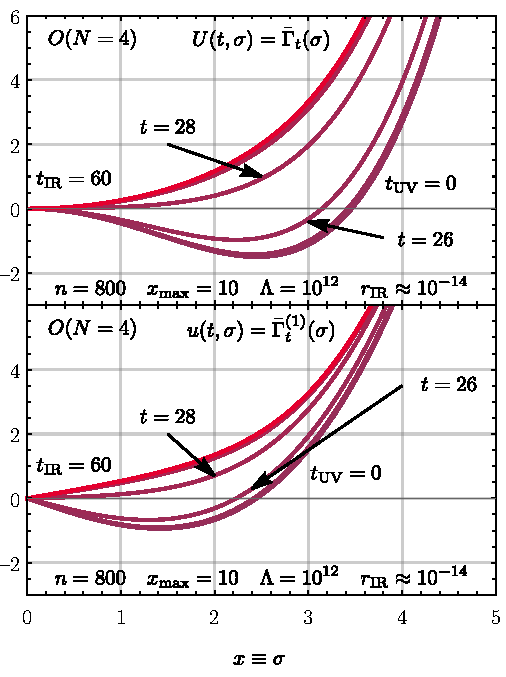
\includegraphics[width=\subcaptionFigureWidth-0.17cm]{0d/figures/sc_ii_n_on_4_n_800_xmax_10_lambda_1e12_tir_60_rg_flow.pdf} % left figure
		\captionsetup{width=\subcaptionFigureWidth-0.17cm}%
		\caption{
			The \frg{} flow of the effective potential $U ( t, \sigma )$ (upper panel) and its derivative $u ( t , \sigma ) = \partial_\sigma U ( t , \sigma )$ (lower panel) for the zero-dimensional $O ( 4 )$ model with \ic{} \eqref{eq:testing_scenario_phi4}, evaluated at $t = 0, \, 2, \, 4, \, \ldots, \, 60$ (integer values for $t$ were chosen for convenience and readability). 
			The (overlapping) {blue} and {violet} curves correspond to the \uv{} and the {red} curves to the \ir{}.
			We used the exponential regulator~\eqref{eq:exponential_regulator} with \uv{} scale $\Lambda = 10^{12}$.
			The plot does not show the region ${x \in[5,10]}$, because the tiny differences between $u ( t, \sigma )$ and $u ( t_\mathrm{UV}, \sigma )$ are not visible in this region and vanish for large $x = \sigma$ anyhow.
			\fromFig{19}{zerod1}
		}
		\label{fig:sc_ii_n_on_4_n_800_xmax_10_lambda_1e12_tir_60_rg_flow}%
	}
	{\fullWidthTwoColumnFigureSpacing}
	{
		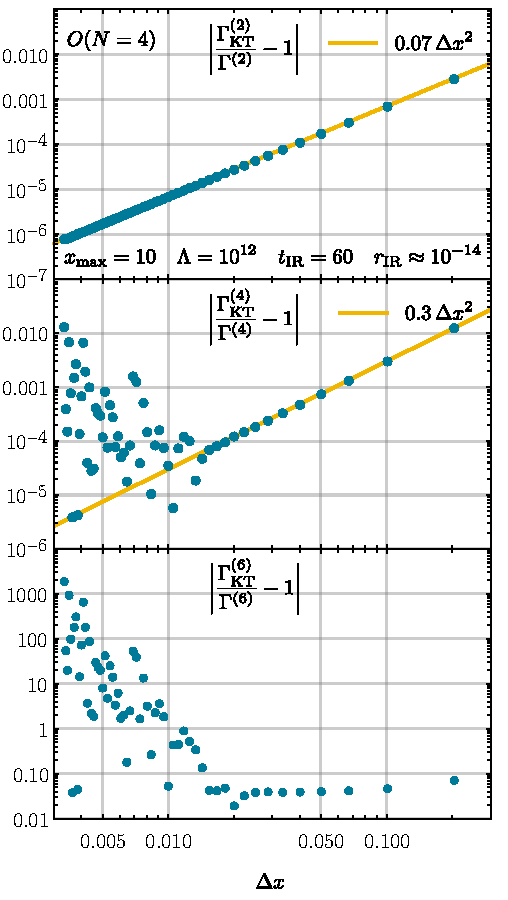
\includegraphics[width=\subcaptionFigureWidth+0.17cm]{0d/figures/sc_ii_n_on_4_xmax_10_lambda_1e12_tir_60_deltax_scaling.pdf} % Right figure
		\captionsetup{width=\subcaptionFigureWidth-0.17cm}%
		\caption{%
			The relative error as a function of the cell size $\Delta x$ for the numerical results (blue dots) from the KT scheme for the coefficients $\Gamma^{(2n)}$ for $n = 1, 2, 3$ with initial potential \eqref{eq:testing_scenario_phi4}.
			The numerical derivatives at $\sigma = 0$ of $u ( t_\mathrm{IR} = 60, \sigma )$ were calculated via the second-order accurate central schemes \eqref{eq:derivative_1_central_error_2}, \eqref{eq:derivative_3_central_error_2}, and \eqref{eq:derivative_5_central_error_2}.
			Here, $x_\mathrm{max} = 10$, but we could have used any sufficiently large $x_\mathrm{max}$.
			We used the exponential regulator~\eqref{eq:exponential_regulator} with \uv{} scale $\Lambda = 10^{12}$.
			The yellow straight lines $\propto \Delta x^2$ are for optical guidance.
			\fromFig{21}{zerod1}%
		}%
		\label{fig:sc_ii_n_on_4_xmax_10_lambda_1e12_tir_60_deltax_scaling}%
	}
In this paragraph we will discuss selected numerical results of the application of the \ktScheme{} for the analytic \ic{} \eqref{eq:testing_scenario_phi4}.
We have performed the full set of numerical tests discussed in \cref{subsubsec:sc1} for this \ic{} and found results supporting the general statements made there.
For brevity, we will not repeat the complete discussion of that subsubsection.
We will limit our discussion to \uv{}/\ir{} scales, the computational domains size ($x_\mathrm{max}$), and its resolution ($\Delta x$). \bigskip

\textbf{\uv{} and \ir{} scales:}
In \cref{fig:sc_ii_n_on_4_n_800_xmax_10_lambda_1e12_tir_60_rg_flow} we present the \frg{} flow of the derivative of the effective potential $u ( t, \sigma )$ from the \uv{} ({blue}) to the \ir{} ({red}).
For the smooth \ic{} \dash{} in the absence of large gradients \dash{} the highly non-linear advection and diffusion contribute almost an equal amount to the dynamics.
Between $t \approx 25$ and $t \approx 30$ we observe significant changes in the shape of the potential: the non-trivial minimum moves towards $\sigma = 0$ and vanishes at $t \approx 28$ resulting in a convex potential with a trivial minimum at $\sigma = 0$ as expected and required.
At small and large $t$ outside the apparent dynamic range between $t \approx 25$ and $t \approx 30$ we observe only very marginal changes in \cref{fig:sc_ii_n_on_4_n_800_xmax_10_lambda_1e12_tir_60_rg_flow}.

A close inspection of the relative errors for the first three non-vanishing \nptFunctions{} in \cref{fig:sc_ii_n_on_4_n_400_xmax_10_lambda_1e12_tir_60_flow_errors} reveals that actually the relevant dynamics sets in much earlier at $t \approx 10$ for the six-point function.
The values for the \nptFunctions{} freeze out at late times around $t \approx 40$, which is due to the diffusion close to $\sigma = 0$.
On the level of $u ( t, \sigma )$ these subtle changes in the \nptFunctions{} cannot be observed by a simple visual inspection of \cref{fig:sc_ii_n_on_4_n_800_xmax_10_lambda_1e12_tir_60_rg_flow}.

The plateaus in the \uv{} (at small $t$) and the \ir{} (at large $t$) support the choice of $\Lambda=10^{12}$ and $t_\mathrm{IR}=60$ to be valid initial \uv{} and \ir{} cutoff scales in terms of \rgcy{}. 
The present \uv{} initial scale is larger when compared to $\Lambda=10^{6}$, which corresponds to $t \approx 14$ in the dynamic region in \cref{fig:sc_ii_n_on_4_n_400_xmax_10_lambda_1e12_tir_60_flow_errors}, used for most computations involving the non-analytic potential considered in the previous \cref{subsubsec:sc1}. 

Hence, the inclusion of a quartic interaction term in \cref{eq:testing_scenario_phi4} seems to require higher \uv{} initial scales to ensure \rgcy{}.
This supports the  statements made in \cref{paragraph:ONRGconsistency}: \rgcy{} and \uv{}/\ir{} scales have to be re-evaluated when changing the \ic{} in the \uv{}, \ie{}, the model under consideration, since characteristic internal scales then also change.\bigskip

\fullWidthTwoColumnFigures%
	[!t] % Placement
	{%
		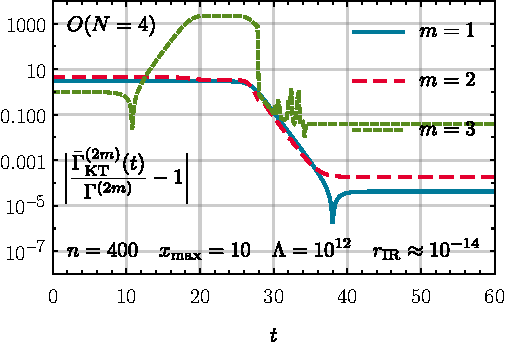
\includegraphics[width=\subcaptionFigureWidth-0.04cm]{0d/figures/sc_ii_n_on_4_n_400_xmax_10_lambda_1e12_tir_60_flow_errors.pdf} % left figure
		\captionsetup{width=\subcaptionFigureWidth-0.04cm}%
		\caption{%
			The relative error for $\Gamma^{(2m)}$, for $m = 1, 2, 3$, calculated with the \ktScheme{} as a function of the \rgtime{} $t$ for the $O(4)$ model.
			The \uv{} initial potential is given by \cref{eq:testing_scenario_phi4}.
			We use the exponential regulator~\eqref{eq:exponential_regulator} with \uv{} scale $\Lambda = 10^{12}$.
			The computational grid has $n=400$ cells and $\sigma_\mathrm{max} = x_\mathrm{max} = 10$.
			$\Gamma^{(2m)}$ are extracted from $u ( t_\mathrm{IR} = 60, \sigma )$ via the finite-difference stencils \eqref{eq:derivative_1_central_error_2}, \eqref{eq:derivative_3_central_error_2}, and \eqref{eq:derivative_5_central_error_2}.
			\fromFig{20}{zerod1}
		}
		\label{fig:sc_ii_n_on_4_n_400_xmax_10_lambda_1e12_tir_60_flow_errors}
	}
	{\fullWidthTwoColumnFigureSpacing}
	{%
		\vspace{-0.2cm}
		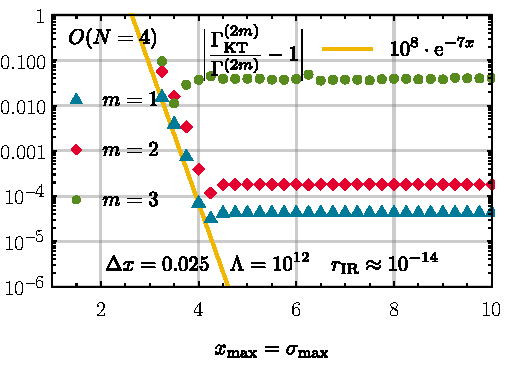
\includegraphics[width=\subcaptionFigureWidth+0.04cm]{0d/figures/sc_ii_n_on_4_deltax_25e-3_lambda_1e12_tir_60_errors_xmax.pdf} % Right figure
		\captionsetup{width=\subcaptionFigureWidth+0.04cm}%
		\caption{%
			The relative error for $\Gamma^{(2m)}$ for $m = 1, 2, 3$ for the \uv{} potential \eqref{eq:testing_scenario_phi4} of the $O ( 4 )$ model as a function of $x_\mathrm{max}$, keeping the cell size $\Delta x = 0.025$ constant.
			$\Gamma^{(2m)}$ are computed from the discrete values of the derivative of the \ir{} potential $u ( t_\mathrm{IR} = 60, \sigma )$ via the second-order accurate central finite-difference stencils \eqref{eq:derivative_1_central_error_2}, \eqref{eq:derivative_3_central_error_2}, and \eqref{eq:derivative_5_central_error_2} at $\sigma = 0$.
			We used the exponential regulator~\eqref{eq:exponential_regulator} with \uv{} scale $\Lambda = 10^{12}$.
			The yellow straight line $\propto\exp\del{-7\,x_\mathrm{max}}$ is for optical guidance.
			\fromFig{22}{zerod1}%
		}%
		\label{fig:sc_ii_n_on_4_deltax_25e-3_lambda_1e12_tir_60_errors_xmax}
	}
\textbf{Size and resolution of the computational domain:} We conclude this paragraph on the \kt{} scheme with a brief discussion regarding the computational domain.
The relative error for the first three non-vanishing \nptFunctions{} is shown as a function of the cell size $\Delta x$ in \cref{fig:sc_ii_n_on_4_xmax_10_lambda_1e12_tir_60_deltax_scaling}.
For the two-point function we recover a perfect error scaling with $\Delta x^2$ down to extremely small $\Delta x$.
The last data point in \cref{fig:sc_ii_n_on_4_xmax_10_lambda_1e12_tir_60_deltax_scaling} is at ${\Delta x \approx 3.3 \cdot 10^{-3}}$ corresponding to $n=3000$ cells.
For the two-point function the rounding errors of the employed finite-difference extraction \eqref{eq:derivative_1_central_error_2} for $\Gamma^{(2)}$ and the finite precision of the \ode{} integrator (\textit{NDSolve} from \WAMXIIwR{} with a \textit{PrecisionGoal} and \textit{AccuracyGoal} of $10$) seem to be small for all depicted $\Delta x$ in this scenario. 
A comparison with the present perfect error scaling for $\Gamma^{(2)}$ supports the comments made about discretization errors for the discontinuous \ic{} \eqref{eq:testing_scenario_non-analytic_quadaratic_asymptote} in \cref{fig:sc_i_on_3_xmax_10_lambda_1e6_tir_60_deltax_scaling}.
For the higher-order \nptFunctions{} $\Gamma^{(4)}$ and $\Gamma^{(6)}$, however, we find that rounding errors related to the finite-difference extractions \eqref{eq:derivative_3_central_error_2} and \eqref{eq:derivative_5_central_error_2} limit the achievable precision.
Again, we identify $\Delta x \approx 0.025$ as an optimal cell size for the extraction of $\Gamma^{(4)}$ and $\Gamma^{(6)}$ but note that typical relative errors for $\Gamma^{(6)}$ are at $\approx 4 \%$ around $\Delta x \approx 0.025$.

In \cref{fig:sc_ii_n_on_4_deltax_25e-3_lambda_1e12_tir_60_errors_xmax}, we study the effect of the size of the computational domain $x_\mathrm{max}$ on the achievable relative errors for $\Gamma^{(2)}$, $\Gamma^{(4)}$, and $\Gamma^{(6)}$ at a constant $\Delta x =0.025$. 
One major difference between the $\phi^4$ potential \eqref{eq:testing_scenario_phi4} studied in this subsubsection and the non-analytic potential~\eqref{eq:testing_scenario_non-analytic_quadaratic_asymptote} of the previous \cref{subsubsec:sc1} is their asymptotic behavior for large $\sigma$.
For large $\sigma$ the leading-order term of the $\phi^4$ potential is \dash{} as the name suggests \dash{} quartic while the non-analytic potential of test case I grows only quadratic.
In terms of the conserved quantity $u = \partial_\sigma U$ one might expect problems when using a linear extrapolation for the ghost cells at large $\sigma$ as discussed in \cref{paragraph:BCinf} with a potential where $u$ grows $\sim \sigma^3$ for large $\sigma$.
For the non-analytic \ic{} \eqref{eq:testing_scenario_phi4} we avoided this possible source of error by construction.
However, considering the results plotted in \cref{fig:sc_ii_n_on_4_deltax_25e-3_lambda_1e12_tir_60_errors_xmax} together with the perfect error scaling displayed in the previous \cref{fig:sc_ii_n_on_4_xmax_10_lambda_1e12_tir_60_deltax_scaling}, we conclude that a linear extrapolation is not problematic even in the case of cubic asymptotics for $u$.
This might be again in part related to the large spatial distance between the physical minimum in the \ir{} and the upper boundary of the grid.
For $x_\mathrm{max}\smallergtrsim 5$ we find a complete insensitivity of the relative errors on the interval size.

\FloatBarrier
\paragraph{\frg{} Taylor expansion: Flow of the $n$-point vertex functions}\phantomsection\label{paragraph:sc2taylorFlow}\mbox{}\\
In this paragraph we confront the theoretical results and concerns stated in \teRef{} and especially in \cref{subsubsec:vertex_expansion} for the zero-dimensional $O(N)$ model \wrt{} the Taylor expansion around the fixed expansion point $\vec{\varphi} = 0$ with the exact results for the zero-dimensional $O(N)$ model.
The $\phi^4$ potential of \cref{eq:testing_scenario_phi4} with negative mass term is the, in terms of \ics{}, simplest \uv{} potential with a non-trivial minimum.
At the end of this subsection we will briefly discuss the Taylor expansion for the $\phi^4$ potential with positive mass term and therefore a scenario without a non-trivial minimum, which has to be considered the simplest non-trivial, \ie{}, interacting, \uv{} \ic{} in the context of the Taylor expansion for the zero-dimensional $O(N)$ model.

In the following we integrate the \ode{} system \eqref{eq:example_vertex_expansion} truncated at $m = 2 n_\mathrm{trunc}$ with the \ic{}
\begin{align}
	\bar{\Gamma}^{(2)} ( 0 ) = - 1 \, ,\qquad \bar{\Gamma}^{(4)} ( 0 ) = + 1 \, ,\qquad \forall n > 2 \quad \bar{\Gamma}^{(2n)} ( 0 ) = 0 \, ,
\end{align}
corresponding to the potential \eqref{eq:testing_scenario_phi4} numerically up to $t_\mathrm{IR}=60$ employing the exponential regulator~\eqref{eq:exponential_regulator} with $\Lambda=10^{12}$ and using the same \ode{} solver \textit{NDSolve} from \WAMXIIwR{} with a \textit{PrecisionGoal} and \textit{AccuracyGoal} of $10$ as before.
Using the \nptFunctions{} at the physical minimum as the flow variables makes an additional extraction procedure (like \acrpllong{fd}) obviously obsolete.
The \nptFunctions{} in the \ir{} can be directly obtained from the values $\bar{\Gamma}^{(2n)} ( t_\mathrm{IR} ) = \Gamma^{(2n)}$.

\fullWidthTwoColumnFigures%
	[!t] % Placement
	{%
		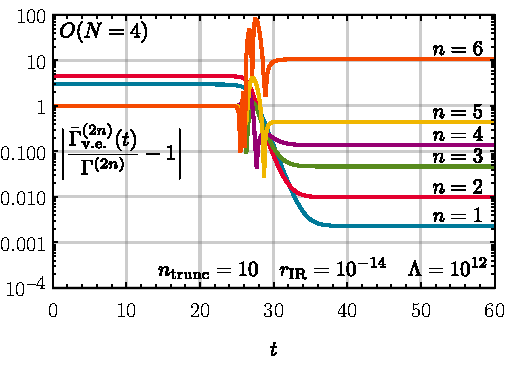
\includegraphics[width=\subcaptionFigureWidth]{0d/figures/sc_ii_n_on_4_lambda_1e12_tir_60_ntrunc_10_vertex_exp_flow.pdf} % left figure
		\captionsetup{width=\subcaptionFigureWidth}%
		\caption{%
			The relative errors for $\Gamma^{(2n)}$ as a function of the \rgtime{} $t$ for $n \in \{ 1, \ldots, 6 \}$ for the $O (4)$ model.
			$\Gamma^{(2n)}$ were calculated via the \frg{} flow of the \frg{} Taylor expansion with truncation order $m = 2 n_\mathrm{trunc} = 20$ using the exponential regulator~\eqref{eq:exponential_regulator}. 
			As initial condition we use the \uv{} potential \eqref{eq:testing_scenario_phi4}.
			\fromFig{23}{zerod1}
		}
		\label{fig:sc_ii_n_on_4_lambda_1e12_tir_60_ntrunc_10_vertex_exp_flow}
	}
	{\fullWidthTwoColumnFigureSpacing}
	{%
		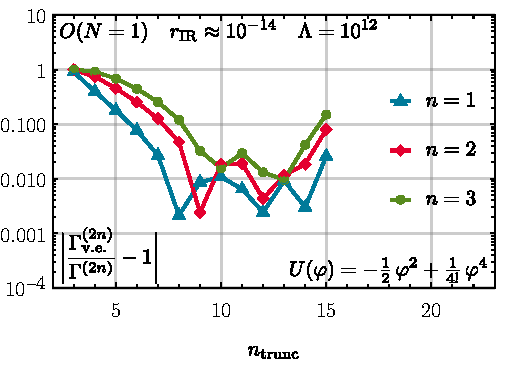
\includegraphics[width=\subcaptionFigureWidth]{0d/figures/sc_ii_n_on_1_lambda_1e12_tir_60_vertex_exp_error.pdf} % Right figure
		\captionsetup{width=\subcaptionFigureWidth}%
		\caption{%
			The relative errors for $\Gamma^{(2n)}$ in the \ir{} for $n = 1, 2, 3$ for the $O (1)$ model, calculated via the \frg{} flow of the \frg{} Taylor expansion to order $m = 2 n_\mathrm{trunc}$ with $n_\mathrm{trunc} \in \{ 3, \ldots , 15 \}$ using the exponential regulator~\eqref{eq:exponential_regulator}.
			As initial condition we use the \uv{} potential \eqref{eq:testing_scenario_phi4}.
			The discrete results for integer $n_\mathrm{trunc}$ are connected by straight lines to improve readability and for a better trend analysis.
			\fromFig{25}{zerod1}%
		}%
		\label{fig:sc_ii_n_on_1_lambda_1e12_tir_60_vertex_exp_error}
	}%
In \cref{fig:sc_ii_n_on_4_lambda_1e12_tir_60_ntrunc_10_vertex_exp_flow} we show the flow of the relative deviations for the first six non-vanishing \nptFunctions{} towards the \ir{} using $m = 2 n_\mathrm{trunc} = 20$ vertices in the expansion for the $O(4)$ model.
We can identify a dynamic range between $t \approx 24$ and $t \approx 38$ in which the vertices vary significantly and change their signs before they reach their respective \ir{} values.
This range is substantially smaller than the dynamic range observed when solving the full \pde{} \eqref{eq:conservation_law_u_phi} using the \ktScheme{}, \cf{} \cref{fig:sc_ii_n_on_4_n_400_xmax_10_lambda_1e12_tir_60_flow_errors}.
In the \ir{}, the errors range from $2.3 \cdot 10^{-3}$ for $\Gamma^{(2)}$ to $1.1 \cdot 10^{1}$ for $\Gamma^{(12)}$.
However, the strict hierarchy observed in \cref{fig:sc_ii_n_on_4_lambda_1e12_tir_60_ntrunc_10_vertex_exp_flow} for $n = 1, \ldots, 6$ is not a general feature of the Taylor expansion for this model.
Using different $n_\mathrm{trunc}$ or including higher-order vertices changes this hierarchy.

\paragraph{\frg{} Taylor expansion: Truncation error}\phantomsection\label{paragraph:sc2taylorError}\mbox{}\\
The truncation error for the $O(4)$ model is discussed using \cref{fig:sc_ii_n_on_4_lambda_1e12_tir_60_vertex_exp_error}, where we show the relative errors for $\Gamma^{(2)}$, $\Gamma^{(4)}$, and $\Gamma^{(6)}$ for the Taylor expansion using different truncation orders $m=2n_\mathrm{trunc}$ between $n_\mathrm{trunc}=3$ and $n_\mathrm{trunc}=14$. 
Beyond $n_\mathrm{trunc}=10$ the relative errors for the \nptFunctions{} no longer decrease and we observe rather strong oscillations for different $n_\mathrm{trunc}$.
The errors for the two and four-point function are with $2.3 \cdot 10^{-3}$ and $9.8 \cdot 10^{-3}$ larger than the errors ($4.2 \cdot 10^{-5}$ and $1.8 \cdot 10^{-4}$ respectively) obtained in the \ktScheme{}, see,  \eg{}, \cref{fig:sc_ii_n_on_4_deltax_25e-3_lambda_1e12_tir_60_errors_xmax}. 
The relative error for the six-point function is with $4.7 \cdot 10^{-2}$ comparable to the $3.7 \cdot 10^{-2}$ error obtained in the \ktScheme{}.
While the extraction of higher-order \nptFunctions{} beyond $n = 6$ is in general possible in the Taylor expansion, their relative errors grow overall rapidly with increasing $n$.

For the \ic{} \eqref{eq:testing_scenario_phi4} we do not observe any meaningful error scaling in orders of $n_\mathrm{trunc}$.
Furthermore a numerical solution at and beyond $n_\mathrm{trunc}=15$ has proven impossible with the current set-up.
At $n_\mathrm{trunc}=15$ an \ode{} integration to the \ir{} at $r ( t_\mathrm{IR} = 60 ) \approx 10^{-14}$ is impossible due to an instability of the \ode{} system occurring at $t \approx 30$ where all coefficients $\Gamma^{(2n)}(t)$ with $n>1$ start diverging.
This divergence seems to be driven by $\Gamma^{(30)}(t)$ for $n_\mathrm{trunc}=15$.
The \ode{} system is in general poorly conditioned since the $\Gamma^{(2n)}(t)$ for different $n$ vary vastly over multiple orders of magnitude.
The instability at  $t \approx 30$ cannot be overcome by increasing the numerical precision of the employed \ode{} integrator (\textit{NDSolve} from \WAMXIIwR{}) and seems to be an inherent problem of the \ode{} systems with $n_\mathrm{trunc}\geq15$.

The Taylor expansion for $\Gamma^{(2n)}(t)$, with a fixed expansion point at $\vec{\varphi} = 0$, for the zero-dimensional $O ( 4 )$ model and the simple \ic{} \eqref{eq:testing_scenario_phi4} with its non-trivial global minimum in the \uv{} is severely limited in its performance.
The absence of a proper error scaling in orders of $n_\mathrm{trunc}$ and the instability of the \ode{} system beyond $n_\mathrm{trunc}=14$ support the conceptual reservations of \teRef{} and \cref{subsubsec:vertex_expansion}.
It seems that the expansion around $\vec{\varphi} = 0$ is either incapable of capturing the dynamics driven by the non-trivial minima located at $| \vec{\varphi} \, | = \sqrt{6}$ in the \uv{} or the desired solution might be non-analytic in $\vec{\varphi} = 0$.

The situation does not improve when considering the same \ic{} in the purely diffusive $O(1)$ model.
In \cref{fig:sc_ii_n_on_1_lambda_1e12_tir_60_vertex_exp_error} we display relative errors for the first three non-vanishing $\Gamma^{(2n)}$ as a function of $n_\mathrm{trunc}$ for the \ic{} \eqref{eq:testing_scenario_phi4} in the $O(1)$ model.
The overall errors are even worse when compared to the $O(4)$ results discussed previously.
The \ode{} integration becomes impossible at $n_\mathrm{trunc} = 16$ where we encounter an instability at $t \approx 31$.

\fullWidthTwoColumnSubFigures%
	[!t]% Placement
	{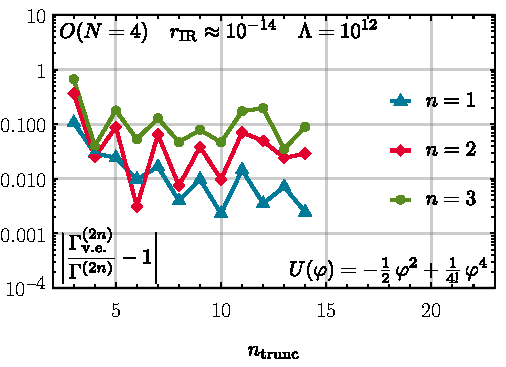
\includegraphics[width=\subcaptionFigureWidth]{0d/figures/sc_ii_n_on_4_lambda_1e12_tir_60_vertex_exp_error.pdf}}% Figure (a)
	{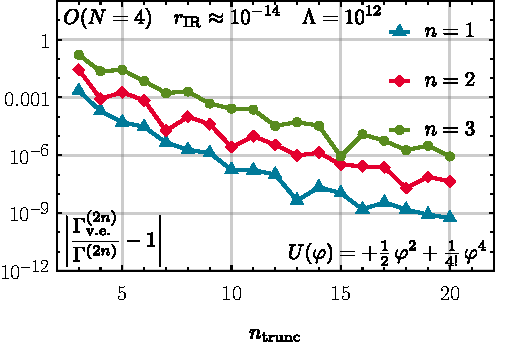
\includegraphics[width=\subcaptionFigureWidth]{0d/figures/sc_ii_p_on_4_lambda_1e12_tir_60_vertex_exp_error.pdf}}% Figure (b)
	[fig:sc_ii_n_on_4_lambda_1e12_tir_60_vertex_exp_error,fig:sc_ii_p_on_4_lambda_1e12_tir_60_vertex_exp_error]% Labels (a) and (b)
	{%
		The relative errors for $\Gamma^{(2n)}$ in the \ir{} for $n = 1, 2, 3$ for the $O (4)$ model, calculated via the \frg{} flow of the Taylor (vertex) expansion to order $m = 2 n_\mathrm{trunc}$ with $n_\mathrm{trunc} \in \{ 3, \ldots , 14 \}$ using the exponential regulator~\eqref{eq:exponential_regulator}.
		As initial condition we use the \uv{} potential \eqref{eq:testing_scenario_phi4} with negative mass term on the left \subref{fig:sc_ii_n_on_4_lambda_1e12_tir_60_vertex_exp_error} and positive mass term on the right \subref{fig:sc_ii_p_on_4_lambda_1e12_tir_60_vertex_exp_error}.
		The discrete results for integer $n_\mathrm{trunc}$ are connected by straight lines to improve readability and for a better trend analysis.
		\fromFigs{24 and 26}{zerod1}%
	}% Caption
	{fig:sc_ii_np_on_4_lambda_1e12_tir_60_vertex_exp_error}% Label	
\paragraph{\frg{} Taylor expansion: $\phi^4$ potential with positive mass term}\phantomsection\label{paragraph:sc2taylorPhiP}\mbox{}\\
We continue our discussion of the \frg{} Taylor expansion by considering the \ic{} \eqref{eq:testing_scenario_phi4} with a positive mass term $+\tfrac{1}{2} \, \vec{\varphi}^{\vts 2}$ and therefore without a non-trivial minimum.
In the context of zero-dimensional $O(N)$ models this \ic{} is in the family of \uv{} potentials discussed qualitatively at length and to some extent even quantitatively in \ccite{Keitel:2011pn,Rosa:2016czs,Moroz:2011thesis}.

In \cref{fig:sc_ii_p_on_4_lambda_1e12_tir_60_vertex_exp_error} we show relative errors for the first three non-vanishing $\Gamma^{(2n)}$ as a function of $n_\mathrm{trunc}$ for this \ic{} for the $O(4)$ model.
These results where obtained using \textit{NDSolve} of \WAMXIIwR{} with an increased \textit{PrecisionGoal} and \textit{AccuracyGoal} of $12$, which became necessary for a proper truncation-error scaling beyond $n_\mathrm{trunc}=15$ for the two-point function.
In \cref{fig:sc_ii_p_on_4_lambda_1e12_tir_60_vertex_exp_error} we observe a truncation-error scaling following power laws in $n_\mathrm{trunc}$ with approximately $n_\mathrm{trunc}^{-8.2}$, $n_\mathrm{trunc}^{-7.6}$, and $n_\mathrm{trunc}^{-7.3}$ for the two-point, four-point, and six-point function respectively.
For this \ic{} the expansion point $\vec{\varphi} = 0$ is located at the global minimum of the potential and the potential is also convex for all $t$.
The dynamics of the \frg{} flow is rather unspectacular for this potential, see Fig.\ 13 of \ccite{Keitel:2011pn} or \cref{fig:sc_ii_p_on=1_n=800_xmax=10_lambda=1.0e12_tir=60_rg_flow} for a visualization.
For the two- and four-point functions, the numerical results at $n_\mathrm{trunc}=3$ ($\Leftrightarrow m=6$) have already acceptable relative errors of $\approx 2.2 \cdot 10^{-3}$ and $\approx 2.8 \cdot 10^{-2}$, respectively, which was observed and discussed in \ccite{Keitel:2011pn}, where results for the Taylor expansions were presented only up to $n_\mathrm{trunc}=3$.
	
The Taylor expansion outperforms the \ktScheme{} in this setting in terms of relative errors.
The performance and practical applicability of the Taylor expansion seem to depend strongly on the \ic{} under consideration.
We will discuss another analytic \ic{} for the Taylor expansion briefly in the next \cref{subsubsec:sc3}.

\paragraph{\frg{} Taylor expansion: Numerical irreversibility}\phantomsection\label{paragraph:sc2taylorIRR}\mbox{}\\
Before we conclude this subsubsection we will briefly comment on the irreversibility of \grg{} flows when employing the \frg{} Taylor expansion.
We discussed in \cref{subsubsec:conservative_form} that the projection onto a finite set of couplings underlying the \frg{} Taylor expansion theoretically allows for an unphysical reversibility of the \grg{} flow.
The \ode{} systems for the running couplings of the \frg{} Taylor expansion in principle allow for an integration both in positive and negative \rgtime{}-direction.
Thus an unphysical resolution of microphysics from macrophysics \dash{} an inversion of the underlying \rg{} transformations connecting them \dash{} is possible when considering a finite set of couplings $\{\bar{\Gamma}^{(2n)}(t)\}$.

We performed practical test with the $\phi^4$ theory discussed in this subsubsection.
For the $\phi^4$ theory with positive mass term discussed in the previous paragraph a complete inversion of the \frg{} flow (from $t=60$ back to $t=0$ using $\Lambda=10^{12}$) is numerically possible for systems with $n_\mathrm{trunc}<7$ for $N=1$.
For larger systems the strong oscillations of the higher-order couplings prevent a numerical integration from the \ir{} back to the \uv{}.
The \ode{} system becomes numerically unstable when approaching $t\approx 24$ from above.
The recovery of the exact \uv{} \ic{} is very good for small $n_\mathrm{trunc}$ but deteriorates when approaching $n_\mathrm{trunc}=7$.
For the $\phi^4$ theory with positive mass term this situations remains qualitatively unchanged for higher $N>1$.

For the $\phi^4$ theory with negative mass term an inversion of the \frg{} flow from the \ir{} to the \uv{} is numerically impossible.
We were not able to find a $n_\mathrm{trunc}$ and $N$ in heuristic tests which allowed for a numerical inversion of the \frg{} flow from $t=60$ back to $t=0$ using $\Lambda=10^{12}$.
The dynamics related to the vaporization of the non-trivial minimum seems to prevent a numerical inversion.
In our heuristic tests it has proven impossible to form back the non-trivial minimum when approaching the \uv{} from the \ir{}.
This is a rather interesting observation which might warrant a detailed investigation of the \ode{} systems involved in the \frg{} Taylor expansion.
Further investigations in higher-dimensional models might be interesting in this context.\bigskip

We will conclude our discussion of the \frg{} Taylor expansion in the next subsubsection with the paragraph \customref{paragraph:sc3taylorConclusion}{FRG Taylor expansion: Concluding remarks}.
\FloatBarrier
\fullWidthTwoColumnFigureTable%
	[t] % Placement
	{0d/figures/sc_iii_uv_initial_condition.pdf} % Figure
	{fig:sc_iii_uv_initial_condition} % Figure label
	{%
		\uv{} potential $U ( \sigma )$ (red-dashed) and its first derivative $u ( \sigma ) = \partial_\sigma U ( \sigma )$ (blue, solid) of test case III from \cref{eq:testing_scenario_phi6}. 
		\fromFig{27}{zerod1}%
	} % Figure caption
	{%
		\renewcommand{\arraystretch}{1.15}
		\small
		\begin{tabular}{l c c c}
			\toprule
			$N$		&	$\Gamma^{(2)}$	&	$\Gamma^{(4)}$	&	$\Gamma^{(6)}$	\\
			\midrule
				$1$	&	$0.174051$	&	$0.015618$	&	$0.013440$\\
				$4$	&	$0.250333$	&	$0.048131$	&	$0.043282$\\
			\bottomrule
		\end{tabular}
	} % Table content
	{tab:sc_3_n_point_functions_exact}% Table label
	{%
		Exact results for $\Gamma^{(2n)}$ of the $O(N)$ model with the \uv{} initial potential \eqref{eq:testing_scenario_phi6} for selected $N$.
		They are obtained by a high-precision one-dimensional numerical integration of the expectation values $\langle ( \vec{\phi}^{\, 2} )^n \rangle$ from \cref{eq:ON_expectation_value} using \textit{NIntegrate} in \WAMXIIwR{}.
		Here, we present the first six digits only.
		\textit{In parts from Tab. III of \ccite{zerod1} and Tab. I of \ccite{zerod2}.}%
	} % Table caption
\subsubsection{Test case III: \texorpdfstring{$\phi^6$}{phi**6} potential}
\label{subsubsec:sc3}
For the third test case we consider the potential
\begin{align}
	U ( \vec{\varphi} \vts ) = \tfrac{1}{2} \, \vec{\varphi}^{\vts 2} - \tfrac{1}{20} \, ( \vec{\varphi}^{\vts 2} )^2 + \tfrac{1}{6!} \, ( \vec{\varphi}^{\vts 2} )^3\, .	\label{eq:testing_scenario_phi6}
\end{align}
This potential includes terms up to $( \vec{\varphi}^{\, 2} )^3$ and has two local minima and one local maximum and is therefore not convex.
The global minimum is located at $\vec{\varphi} = 0$ and the potential and its derivative (evaluated on the constant field configuration $\sigma$) are depicted in \cref{fig:sc_iii_uv_initial_condition}.
Selected reference values for the first three non-vanishing \nptFunctions{} can be found in \cref{tab:sc_3_n_point_functions_exact}.

We have again performed the full set of numerical tests of \cref{subsubsec:sc1} and found results supporting the general statements made in that subsection.
For brevity, we will not repeat the complete discussion of that subsubsection but instead focus again on selected results.\bigskip

\Cref{fig:sc_iii_on_4_n_800_xmax_10_lambda_1e12_tir_60_rg_flow} shows the \frg{} flow with the initial condition \eqref{eq:testing_scenario_phi6} for the $O(4)$ model computed with the \ktScheme{} again using \textit{NDSolve} of \WAMXIIwR{} with \textit{PrecisionGoal} and \textit{AccuracyGoal} of 10 for the \frg{} time evolution.
Both non-trivial local extrema fade away during \frg{} time evolution towards the \ir{}.
At $t \approx 28$ the potential $U ( t, \sigma )$ becomes convex as $u ( t, \sigma )$ turns strictly positive for $\sigma > 0$.
We again observe that the linear extrapolation used at the right boundary $x_\mathrm{max}$ of the computational domain seems surprisingly efficient even for an initial condition with quintic asymptotics.
Studying \cref{fig:sc_iii_on_4_deltax_25e-3_lambda_1e12_tir_60_errors_xmax} we observe that the relative errors in the \ir{} become independent of the size of the computational domain for $x_\mathrm{max}\smallergtrsim 6$.

\fullWidthTwoColumnFigures%
	[!t] % Placement
	{%
		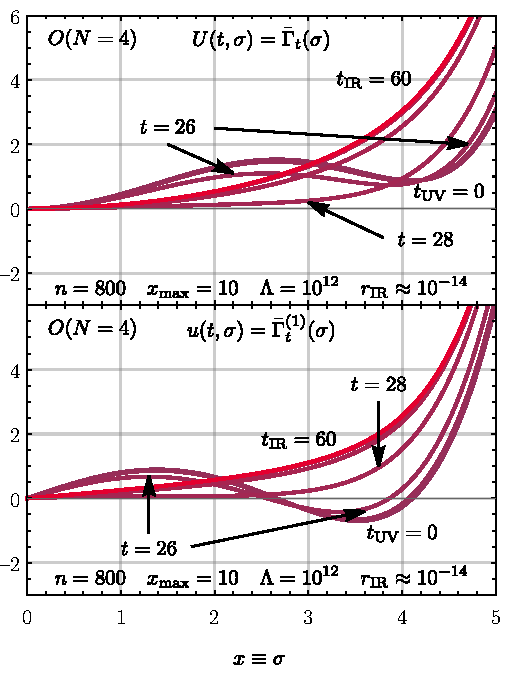
\includegraphics[width=\subcaptionFigureWidth]{0d/figures/sc_iii_on_4_n_800_xmax_10_lambda_1e12_tir_60_rg_flow.pdf} % left figure
		\captionsetup{width=\subcaptionFigureWidth}%
		\caption{
			The \frg{} flow of the effective potential $U ( t, \sigma )$ (upper panel) and its derivative $u ( t , \sigma ) = \partial_\sigma U ( t , \sigma )$ (lower panel) for the zero-dimensional $O ( 4 )$ model with initial condition \cref{eq:testing_scenario_phi6}, evaluated at $t = 0, \, 2, \, 4, \, \ldots, \, 60$ (integer values for $t$ were chosen for convenience and readability). 
			The (overlapping) {blue} and {violet} curves correspond to the \uv{} and the {red} curves to the \ir{}.
			We used the exponential regulator~\eqref{eq:exponential_regulator} with \uv{} scale $\Lambda = 10^{12}$.
			The plot does not show the region ${x \in[5,10]}$, because the tiny differences between $u ( t, \sigma )$ and $u ( t_\mathrm{UV}, \sigma )$ are not visible in this region and vanish for large $x = \sigma$ anyhow.
			\fromFig{28}{zerod1}
		}
		\label{fig:sc_iii_on_4_n_800_xmax_10_lambda_1e12_tir_60_rg_flow}%
	}
	{\fullWidthTwoColumnFigureSpacing}
	{
		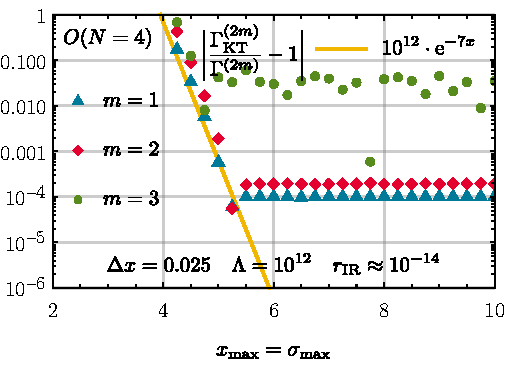
\includegraphics[width=\subcaptionFigureWidth]{0d/figures/sc_iii_on_4_deltax_25e-3_lambda_1e12_tir_60_errors_xmax.pdf} % Right figure
		\captionsetup{width=\subcaptionFigureWidth}%
		\caption{%
			The relative error for $\Gamma^{(2m)}$ for $m = 1, 2, 3$, for the $O ( 4 )$ model using the \uv{} potential \eqref{eq:testing_scenario_phi6}, as a function of the size of the computational interval $x_\mathrm{max}$. The cell size is $\Delta x = 0.025$. $\Gamma^{(2m)}$ are computed from the discrete values of the derivative of the \ir{} potential $u ( t_\mathrm{IR} = 60, \sigma )$ via the second-order accurate central finite-difference stencils \eqref{eq:derivative_1_central_error_2}, \eqref{eq:derivative_3_central_error_2}, and \eqref{eq:derivative_5_central_error_2} at $\sigma = 0$.
			We used the exponential regulator~\eqref{eq:exponential_regulator} with \uv{} scale $\Lambda = 10^{12}$.
			The yellow straight line $\propto\exp\del{-7\,x_\mathrm{max}}$ is for optical guidance.
			\fromFig{29}{zerod1}%
		}%
		\label{fig:sc_iii_on_4_deltax_25e-3_lambda_1e12_tir_60_errors_xmax}%
	}
\paragraph{\frg{} Taylor expansion: Concluding remarks}\phantomsection\label{paragraph:sc3taylorConclusion}\mbox{}\\
We were not able to evolve the \ode{} system of the Taylor expansion with the current initial condition to the \ir{} for any setup at all\footnote{%
	We thank J.~Eser for discussions on this issue and a cross-check using his \frg{} Taylor expansion code~\cite{Divotgey:2019xea,Cichutek:2020bli,Eser:2018jqo,Eser:2019pvd}, which reproduced our findings.
}. 
Independent of $n_\mathrm{trunc}$ and \ode{} integrator (\textit{NDSolve} of \WAMXIIwR{}) settings we encounter a numerical instability of the \ode{} systems at around $t \approx 28$ preventing a complete integration to the \ir{}.
The expansion coefficients $\bar{\Gamma}^{(2n)}(t)$ simply diverge at $t \approx 28$.
From \cref{fig:sc_iii_on_4_n_800_xmax_10_lambda_1e12_tir_60_rg_flow} we deduce that this is approximately the \rgtime{} point at which the non-trivial extrema vanish and the potential turns convex.
The precise underlying dynamics generated by the full \pde{} and resolved by the \ktScheme{} cannot be captured by the Taylor expansion (at least not in our set-up). 
However, also switching to a set-up with a $t$-dependent expansion point will not cure this problem, because the expansion point (the global minimum) does not move for this initial potential \dash{} a conscious design decision for test case III.
The instability of the solution of the coupled system of \odes{} might be explained \aposteriori{} by the formation of a non-analyticity at or around the \rgtime{} $t \approx 28$ of the collapse of the expansion.
Inevitably, due to the non-analyticity of the potential, Wilbraham-Gibbs-type~\cite{Wilbraham:1848,Gibbs:1898,Gibbs:1899} oscillations arise in the Taylor expansion, making the expansion scheme unstable~\cite{boyd2001chebyshev}.
This phenomenon is also observed and discussed in detail in the context of Fourier expansions of periodic potentials in the \frg{} in Sec.~2.2.2 of \ccite{Pangon:2010uf}.

However, a vertex expansion for a convex sextic potential including only positive coefficients in the \uv{} is possible, similar to $\phi^4$ theory with a positive mass term discussed at the end of the previous \cref{paragraph:sc2taylorPhiP}.
A numerical inversion of the \frg{} flow is again possible for systems with a small number of couplings.\bigskip

At this point we have discussed numerical results for the \frg{} Taylor expansion for quartic and sextic potentials.
The numerical performance in terms of achievable relative errors for the \nptFunctions{} in the \ir{} is rather poor for the quartic potential \eqref{eq:testing_scenario_phi4} with the negative mass term and very good for the potential with the positive mass term.
A numerical solution of \ode{} system of the Taylor expansion with the non-convex sextic potential \eqref{eq:testing_scenario_phi6} has proven impossible 

The zero-dimensional $O(N)$ model has proven very challenging for the Taylor expansion.
It seems that only convex, analytic \uv{} initial conditions and the resulting rather simple \frg{} flows can be treated with a vertex expansion in $\bar{\Gamma}^{(2n)}(t)$ around $\vec{\varphi} = 0$ in the zero-dimensional $O(N)$ model.

At this point we also want to reference our comments in \cref{sububsec:LAEBBE}: the treatment of non-linear advection-diffusion equations requires \apriori{} shock capturing schemes, capable of handling non-analyticities and even discontinuities.
An application of expansion schemes relying on analyticity like the Taylor expansion is only possible in very special situations and require an \aposteriori{} case-by-case evaluation of the method.
In scenarios where the \frg{} flows are driven by an interplay of advection and diffusion around non-trivial minima and/or large gradients of the conserved quantity $u$, the Taylor expansion is inevitably doomed to fail.
It is not possible to capture the dynamics of such equations reliably with the simple Taylor expansion discussed here.
A numerical inversion of the \grg{} flow is also impossible in those scenarios.
The appearance of a non-analytic behavior is also understood via a rise of entropy, \cf{} \cref{subsubsec:0dO1entResults,paragraph:infiniteNflowsEntropy}.

It should be noted that in this work we discussed the simplest possible Taylor/vertex-expansion scheme.
Other versions of the \frg{} Taylor (vertex) expansion including a moving expansion point or a rescaling of the expansion coefficients might improve the performance of the expansion scheme in certain cases, \cf{} \ccite{Litim:2002cf,Schaefer:2001cn,Rennecke:2015lur}.
Implementing and testing different approaches to the Taylor expansion for zero-dimensional $O(N)$ models would certainly be an interesting topic for further studies.
\FloatBarrier
\fullWidthTwoColumnFigureTable%
	[t] % Placement
	{0d/figures/sc_iv_uv_initial_condition.pdf} % Figure
	{fig:sc_iv_uv_initial_condition} % Figure label
	{%
		\uv{} potential $U ( \sigma )$ (red-dashed) and its first derivative $u ( \sigma ) = \partial_\sigma U ( \sigma )$ (blue, solid) of test case IV from \cref{eq:testing_scenario_4}. 
		\fromFig{30}{zerod1}%
	} % Figure caption
	{%
		\renewcommand{\arraystretch}{1.15}
		\small
		\begin{tabular}{l c c c}
			\toprule
			$N$		&	$\Gamma^{(2)}$	&	$\Gamma^{(4)}$	&	$\Gamma^{(6)}$	\\
			\midrule
			$1$	&	$0.204698$	&	$0.064682$	&	$0.112849$\\
			$3$	&	$0.421674$	&	$0.153559$	&	$0.249252$\\
			\bottomrule
		\end{tabular}
	} % Table content
	{tab:sc_4_n_point_functions_exact}% Table label
	{%
		Exact results for $\Gamma^{(2n)}$ of the $O(N)$ model with the \uv{} initial potential \eqref{eq:testing_scenario_4} for selected $N$.
		They are obtained by a high-precision one-dimensional numerical integration of the expectation values $\langle ( \vec{\phi}^{\, 2} )^n \rangle$ from \cref{eq:ON_expectation_value} using \textit{NIntegrate} in \WAMXIIwR{}.
		Here, we present the first six digits only.
		\textit{In parts from Tab. IV of \ccite{zerod1} and Tab. I of \ccite{zerod2}.}%
	} % Table caption
\subsubsection{Test case IV: The \texorpdfstring{$\sigma\mkern-2mu=\mkern-2mu0$}{sigma=0} boundary}
\label{subsubsec:sc4}
The last test case is again a non-analytic and discontinuous potential,
\begin{align}
	U ( \vec{\varphi} \vts ) =
	\begin{cases}
		- ( \vec{\varphi}^{\vts 2} )^{\tfrac{1}{3}} \, ,			&	\text{if} \quad |\vec{\varphi}| \leq \sqrt{8} \, ,\\
		\tfrac{1}{2} \, \vec{\varphi}^{\vts 2} - 6 \, ,							&	\text{if} \quad |\vec{\varphi}| > \sqrt{8} \, .
	\end{cases}	\label{eq:testing_scenario_4}
\end{align}
The numerically challenging features are the cusp at $\varphi = 0$ as well as a non-trivial minimum at the kink at $\varphi = \sqrt{8}$.
As displayed in \cref{fig:sc_iv_uv_initial_condition} (evaluated on the constant field configuration), the cusp\footnote{
	Potentials with cusps in field space are not just academic thought experiments.
	They are encountered in, \eg{}, theories in $2+1$ space-time dimensions, such as the Gross-Neveu model~\cite{Braun:2010tt}.
} at $\sigma = 0$ in $U(\sigma)$ translates to a pole in $\partial_\sigma U(\sigma)\equiv u(\sigma)$.
This scenario was engineered as an extreme test case for the boundary condition at $\sigma = 0$ discussed at length in \cref{paragraph:BC0}.

We have again performed the full set of numerical tests of \cref{subsubsec:sc1} and found results supporting the general statements made in \cref{subsubsec:sc1}.
For brevity, we will not repeat the complete discussion of that subsubsection but instead focus again on selected results.\bigskip

\subcaptionFigureOneTwo%
	[!t]% placement
	{0d/figures/sc_iv_on_3_n_800_xmax_10_lambda_1e8_tir_60_rg_flow.pdf}% figure (a)
	{%
		\caption{
			The \frg{} flow of the effective potential $U ( t, \sigma )$ (upper panel) and its derivative $u ( t , \sigma ) = \partial_\sigma U ( t , \sigma )$ (lower panel) evaluated at $t = 0, \, 2, \, 4, \, \ldots, \, 60$ (integer values for $t$ were chosen for convenience and readability). 
			The (overlapping) {blue} and {violet} curves correspond to the \uv{} and the {red} curves to the \ir{}.
			We used the exponential regulator~\eqref{eq:exponential_regulator} with \uv{} scale $\Lambda = 10^{8}$ and $n = 800$ volume cells.
			The plot does not show the region ${x \in[5,10]}$, because the tiny differences between $u ( t, \sigma )$ and $u ( t_\mathrm{UV}, \sigma )$ are not visible in this region and vanish for large $x = \sigma$ anyhow.
		}%
		\label{fig:sc_iv_on_3_n_800_xmax_10_lambda_1e8_tir_60_rg_flow}%
	}% caption/label (a)
	{%
		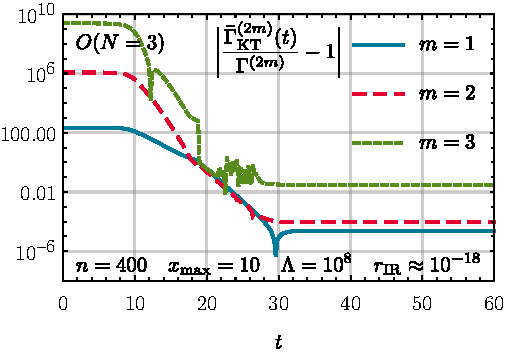
\includegraphics[width=\subcaptionFigureWidth]{0d/figures/sc_iv_on_3_n_400_xmax_10_lambda_1e8_tir_60_flow_errors.pdf}
		\caption{
			The relative error for $\Gamma^{(2m)}(t)$, for $m = 1, 2$, calculated with the \ktScheme{} as a function of the \rgtime{} $t$ for the $O(3)$ model.
			We used the exponential regulator~\eqref{eq:exponential_regulator} with \uv{} scale $\Lambda = 10^{8}$ and $n = 400$ volume cells.
		}%
		\label{fig:sc_iv_on_3_n_400_xmax_10_lambda_1e8_tir_60_flow_errors}%
	}% figure/caption/label (b)
	{%
		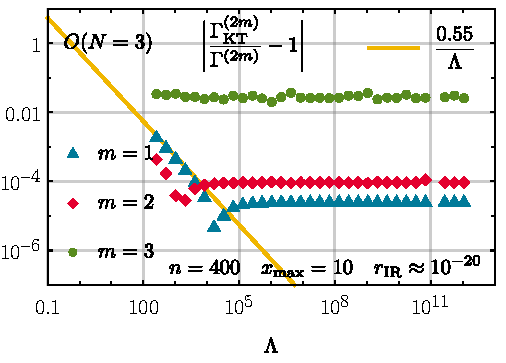
\includegraphics[width=\subcaptionFigureWidth]{0d/figures/sc_iv_on_3_n_400_xmax_10_rir_10e-20_cutoff_test.pdf}
		\caption{
			The relative error for $\Gamma^{(2m)}(t_\mathrm{IR})$ for $m = 1, 2, 3$ from the \ktScheme{} as a function of the \uv{} scale scale $\Lambda$.
			We use the exponential regulator~\eqref{eq:exponential_regulator} and keep the \ir{} cutoff scale constant at $r(t_\mathrm{IR}) = 10^{-15}$ for all runs.
			The number of volume cells is $n = 400$.
			The straight yellow line $\propto \Lambda^{-1}$ is for optical guidance.
		}%
		\label{fig:sc_iv_on_3_n_400_xmax_10_rir_10e-20_cutoff_test}%
	}% figure/caption/label (c)
	{%
		\Frg{} flow on the left \subref{fig:sc_iv_on_3_n_800_xmax_10_lambda_1e8_tir_60_rg_flow}, relative errors over \rgtime{} on the top right \subref{fig:sc_iv_on_3_n_400_xmax_10_lambda_1e8_tir_60_flow_errors}, and relative errors in the \ir{} as function of the \uv{} cutoff $\Lambda$ on the bottom right \subref{fig:sc_iv_on_3_n_400_xmax_10_rir_10e-20_cutoff_test} for the zero-dimensional $O ( 3 )$ model with initial condition \cref{eq:testing_scenario_4}.
		The computational grid size is $\sigma_\mathrm{max} = x_\mathrm{max} = 10$ and $\Gamma^{(2m)}(t)$ are calculated from $u ( t, \sigma )$ via the approximations \eqref{eq:derivative_1_central_error_2}, \eqref{eq:derivative_3_central_error_2}, and \eqref{eq:derivative_5_central_error_2} for the numerical derivatives.
		\fromFigs{31, 32, and 33}{zerod1}%
	}% caption
	{fig:sc_iv_flows}% label
\Cref{fig:sc_iv_on_3_n_800_xmax_10_lambda_1e8_tir_60_rg_flow} depicts the \frg{} flow for the $O(3)$ model computed with the \ktScheme{} for the \uv{} initial condition \eqref{eq:testing_scenario_4}.
\Cref{fig:sc_iv_on_3_n_400_xmax_10_lambda_1e8_tir_60_flow_errors} displays the corresponding flow of the first three non-vanishing \nptFunctions{}.
With our implementation of the \ktScheme{} using \textit{NDSolve} of \WAMXIIwR{} with a \textit{PrecisionGoal} and \textit{AccuracyGoal} of $10$ we are able to compute precise solutions, where the achievable precision for $\Gamma^{(4)}$ and $\Gamma^{(6)}$ is, as discussed in the previous subsubsections, limited by the finite-difference rounding errors.
The discretization-error scaling shows the same peculiarities as the test case I of \cref{subsubsec:sc1} due to the discontinuities in the initial conditions.
The corresponding  reference values for the $O(3)$ model are listed in \cref{tab:sc_4_n_point_functions_exact}.
The dynamics during the \frg{} flow is dominated by the pole at $\sigma = 0$ and the discontinuity at $\sigma = \sqrt{8}$ in $u(\sigma)$.
The diffusion smears out the discontinuity and advection transports it towards $\sigma = 0$ ``filling up the well'' at $\sigma = 0$.
Considering the corresponding values for $u(\sigma)$ for $\sigma < 0$ using the antisymmetry of $u(\sigma)$, the boundary at $\sigma = 0$ can be seen as a point where waves of opposite amplitude annihilate \dash{} a situation very reminiscent of our discussion of the \bbeq{} in \cref{paragraph:BBE}.

Only the carefully engineered boundary condition at $\sigma = 0$ together with corresponding ghost cells allows for practical computations with the present initial condition.
The pole at $\sigma = 0$ presents no problem in practical computations because the boundary condition at $\sigma = 0$ makes use of the antisymmetry of $u ( t, \sigma )$. 
The first cell containing the pole is centered at $\sigma = 0$ and due to the antisymmetry, the corresponding cell average $\bar{u}_0(t)$ vanishes by construction.
Enforcing $\bar{u}_0(t)=0$ and for the two ghost cells $\bar{u}_{-2}(t)=-\bar{u}_{2}(t)$ and $\bar{u}_{-1}(t)=-\bar{u}_{1}(t)$ at each time step allows for a stable and accurate \frg{} time evolution even for such extreme initial conditions like the one of \cref{eq:testing_scenario_4}.

Treating this initial condition using a formulation in the invariant $\varrho = \tfrac{1}{2} \, \sigma^2$ with some naive boundary conditions without strict mathematical justification is hazardous, because $u ( t, \varrho ) = \partial_\varrho U ( t, \varrho )$ diverges as $\varrho^{-2/3}$ as $\varrho \rightarrow 0$.
As mentioned in \cref{paragraph:BC0}, it is unclear to us how to deal with the $\varrho = 0$ boundary especially in a case like the one discussed in this subsubsection.\bigskip

We conclude this subsection with a short discussion of \rgcy{}.
The plateaus in \cref{fig:sc_iv_on_3_n_400_xmax_10_lambda_1e8_tir_60_flow_errors} in the \uv{} (at small $t$) and the \ir{} (at large $t$) are again a strong indication for appropriately chosen \uv{} and \ir{} scales.
From \cref{fig:sc_iv_on_3_n_400_xmax_10_rir_10e-20_cutoff_test}, showing the $\Lambda$-dependence of $\Gamma^{(2)}$, $\Gamma^{(4)}$, and $\Gamma^{(6)}$, one observes that, even in the presence of the pole at $\sigma = 0$ in ${u ( t = 0, \sigma )}$, an initial \uv{} scale of $\Lambda=10^8$ is sufficient to realize \rgcy{}. 
Arguably even $\Lambda=10^6$ \dash{} the scale used in \cref{subsubsec:sc1} \dash{} would suffice, suggesting that in the current case the scale is primarily set by the discontinuity and linear asymptotics at and beyond $\sigma = \sqrt{8}$, which both are also present (with very similar values) in the initial condition \eqref{eq:testing_scenario_non-analytic_quadaratic_asymptote} of \cref{subsubsec:sc1}.

However, decreasing $\Delta x$ would lead to larger numerical gradients for the initial condition at $\sigma = 0$ due to the discretization of the pole in $u(\sigma)$, which in turn implies that $\Lambda$ has to be simultaneously increased in order to keep the propagators \eqref{eq:advection_flux_pion_propagator} and \eqref{eq:diffusion_flux_sigma_propagator} dominated by $\Lambda$ in the \uv{}.

Also, if the cusp at $\sigma = 0$ in the \uv{} initial potential $U ( t = 0, \sigma )$ in \cref{fig:sc_iv_uv_initial_condition} pointed downwards and $u ( 0, x )$ had negative gradients on both sides of the corresponding pole, it would formally be extremely hard to guarantee the inequalities \eqref{eq:LambdaMin} and to have a non-singular flow equation in the \uv{}, because the giant negative gradients would not be restricted to the cell at $\sigma = 0$.
In a discretized version with non-zero $\Delta x$ a calculation is still possible, as long as $\Lambda$ is chosen extremely large, much larger than the huge, but finite negative gradient of $u(\sigma)$.
Hence, \rgcy{} is not only a physical requirement, but also sets strict limits on the choice of numerical parameters, respectively.
We observe similar effects in \cref{paragraph:chemical_potential_shock_wave}, where the chemical potential enters as a shock wave in field space with (at $T=0$) infinite negative slope in $u(t,\sigma)$ at positive $\sigma$.
	
\FloatBarrier
\subsection{The \ONn{1} model -- entropy production and irreversibility of RG flows}\label{subsec:0dO1Entropy}
\begin{disclaimer}
	This subsection is based on \ccite{Koenigstein:2021rxj} and contains parts of the unpublished notes~\cite{Koenigstein:fixedPoint}.
	The plots of \ccite{Koenigstein:2021rxj} and the underlying numerical data were produced by A. Koenigstein and numerically cross-checked by my own computations with the KT scheme.
	
	Selected numerical results and accompanying symbolic computations are included in the digital auxiliary file~\cite{Steil:2023zeroDN1}.
	The single thread wall time on an \intel{} for the numeric results of this subsection is only around eight minutes, since we only discuss five \frg{} trajectories.
	
	The introduction of this subsection follows Secs. I and II of \ccite{Koenigstein:2021rxj}.
\end{disclaimer}
In this subsection we will focus on $O(N=1)$ models, \ie{}, a zero-dimensional \ZII{}-symmetric model of a single scalar, as discussed especially at the beginning of this chapter in \cref{sec:0dQFT}.
In the spirit of \cref{paragraph:conservative_form_diffusion}, the limitation to $N=1$ entails, that the flow equation gets purely diffusive as the advective contributions $\propto(N-1)$ vanish.
We are left with the scalar parabolic conservation law,
\begin{align}
	\partial_t U ( t, \sigma ) = \frac{1}{2} \,\frac{1}{r ( t ) + \partial_\sigma^2 U ( t, \sigma )}\, \partial_t r ( t ) = %
	\input{0d/diagrams/SU2model0d-Uflow_00014_1.tex}\, ,	\label{eq:o(1)_wetterich_equation}
\end{align}	
which in primitive form reads
\begin{align}
	\partial_t u ( t, x ) = \, & \alpha[t,\partial_x u ( t, x )] \, \partial_x^2 u ( t, x ) \, ,\label{eq:0ddifprimII}
\end{align}
with the non-linear, strictly positive diffusion coefficient
\begin{align}
	\alpha[t,\partial_x u ( t, x )] \equiv - \frac{\tfrac{1}{2} \, \partial_t r ( t )}{[ r ( t ) + \partial_x u ( t, x ) ]^2} \, ,	\label{eq:diffusion_coefficientII}
\end{align}
\cf{} \cref{eq:0ddifprim,eq:diffusion_coefficient}.
We can identify \cref{eq:0ddifprimII} as a heat equation with non-linear diffusion coefficient \eqref{eq:diffusion_coefficientII}, \cf{} \cref{subsec:hydroDiffusion}.
The present discussion makes our general remarks about functional flow/heat equations in \cref{subsec:RGflow} explicit.
The conservative formulation \eqref{eq:o(1)_wetterich_equation} and interpretation in terms of (numerical) fluid dynamics has tremendous benefits and consequences for understanding and solving this \frg{} flow equation:
	\begin{enumerate}
		\item	The explicit identification of the \frg{} flow \cref{eq:o(1)_wetterich_equation} as a heat equation allows us to directly apply the \cfd{} methods of \cref{sec:conservationLaws} and especially \cref{subsec:hydroDiffusion}.
		\item	An interpretation of \frg{} flow equations as flow equations in the narrow sense of the word makes the dynamics during the flow intuitively understandable.
		The non-linear diffusive contribution (the radial \sigmaMode{}) smears out cusps and jumps in $u ( t, x )$ and corresponds to undirected movement of $u ( t, x )$, depending on the local ``concentration differences'', the gradient $\partial_x u ( t, x )$, via the highly non-linear diffusion coefficient \eqref{eq:diffusion_coefficientII}.
		\item The described dissipative dynamics goes hand in hand with entropy production and irreversibility as discussed in the \cfd{} context in \cref{subsec:hydroDiffusion}.
		We can therefore conclude that the irreversibility of the \rg{} transformations during the \frg{} flow is hard coded in the diffusive character of the flow \cref{eq:o(1)_wetterich_equation}, not only in zero space-time dimensions, but for any dimension and any \qft{}, \cf{}\ \ccite{Zumbach:1994kc,Zumbach:1994kc,Zumbach:1994vg,Zumbach:1993zz}.
		Hence, the rise of entropy during the \frg{} flow might therefore be directly linked to $\mathcal{C}$-/$\mathcal{A}$-theorems.
		This is explained in detail in this subsection in the context of our minimalistic toy model \qft{}.
	\end{enumerate}

To be specific, we shall show that the numerical entropy, which is of utmost importance in the theoretical treatment of \pdes{}, as outlined in \cref{sec:conservationLaws} and especially \cref{subsec:hydroKT}, has a very close connection to an entropy in the \grg{} flow\footnote{In this context we also have to mention the publication~\cite{Cotler:2022fze} by J. Cotler and S. Rezchikov, who were able to interpret the Polchinski equation as an ``optimal transport gradient flow of a field-theoretic relative entropy'', thus establishing a firm and explicit connection between an information-theoretic entropy and \grg{} flows.} and further possible connections to the so-called $\mathcal{C}$-/$\mathcal{A}$-functions, \cf{}\ \ccite{Zamolodchikov:1986gt,Rosten:2010vm,Banks:1987qs,Cardy:1988cwa,Osborn:1989td,Jack:1990eb,Komargodski:2011vj,Curtright:2011qg,Haagensen:1993by,Generowicz:1997he,Forte:1998dx,Codello:2013iqa,Codello:2015ana,Becker:2014pea,Becker:2016zcn} and \cref{subsubsec:c-theorem_irreversibility_entropy} for more details on $\mathcal{C}$-/$\mathcal{A}$-functions.

One of the most important direct consequences of this is, that the same ``(thermodynamic) arrow of time'' or ``thermodynamic time asymmetry''~\cite{Lebowitz:2008} identified by the entropy of a \pde{}, is also present from a \frg{} perspective.

In nature as well as in the \pdes{} that describe our physical world, entropy is produced by diffusion (dissipation) as well as discontinuities of different kinds.
Consequently the evolution of such systems and also their numerical solutions are irreversible and usually only weak solutions are accessible numerically~\cite{Lax1973,Ames:1992,LeVeque:1992,LeVeque:2002,Hesthaven2007,Toro2009,RezzollaZanotti:2013}.
As we will demonstrate in this subsection, the \acrrepeat{tvni} property and related numerical entropy, \cf{} \cref{eq:TVcontinuous} and the subsequent discussions of \cref{sec:conservationLaws}, used to guarantee the stability of numeric solution schemes, can be promoted to a ``physical'' entropy function.
This entropy function shares characteristics with a $\mathcal{C}$-function and its properties transfer from the \pde{} to the \qft{} and vice versa.
Therefore, \grg{} flows are also not reversible.\footnote{Note that similar arguments, which link the dissipative character of \rg{} flow equations to the irreversibility of the \rg{} flow, were already brought up in \ccite{Zumbach:1994vg,Zamolodchikov:1986gt} already before or parallel to the development of the functional \rg{} framework pioneered in \ccite{Wetterich:1992yh}.} This makes the semi-group character of the \rg{}, see, \eg{}, \ccite{deligne1999quantum}, explicit.
This semi-group character manifests very explicitly in Kadanoff's block-spin picture~\cite{Kadanoff:1966wm,Wilson:1971bg,Wilson:1971dh,Wilson:1979qg} \dash{} it is intuitively obvious that the averaging over a set of spins is an irreversible process.
The irreversibility of \grg{} flows is not just an abstract concept, but is present on a practical level in rather simple truncations of the Wetterich equation. 

These statements may have no severe practical implications for studies of, \eg{}, \qcd{} and condensed-matter systems, where the \grg{} flow is in general  followed from small (\uv{} limit) to large length scales (\ir{} limit).
In these cases, the dynamics in the long-range limit is predicted from a given known \uv{} action by integrating out high momentum modes along the ``natural'' \rgtime{}-direction.
However, in situations where \grg{} flows are followed from large to small length scales, such as studies of the asymptotic safety scenario in \qfts{} (see \ccite{Weinberg:1976xy,Weinberg:1996kw,Percacci:2007sz,Weinberg:2009ca,Rosten:2010vm} in general, \ccite{Niedermaier:2006wt,Bonanno:2020bil} for a recent review in the context of (quantum) gravity, and \ccite{Braun:2010tt,Jakovac:2014lqa} for applications in condensed-matter physics), the question of irreversibility of \grg{} flows and the associated production of entropy may indeed be very relevant.

Whereas \frg{} flows are indeed reversible for certain classes of truncations (of the underlying effective action), we shall demonstrate in the present work \dash{} with the aid of simple models \dash{} that it becomes formally impossible to reverse \frg{} flows in cases where no truncations of the effective action are made.
Even more, already for often employed truncation schemes (\eg{}, \lpa{}), we shall see that irreversibility associated with numerical entropy production can already be a manifest feature of \frg{} flows.
Of course, irreversibility of \frg{} flows does not imply, that it is not possible to construct theories, which are valid on all scales.
It only implies, that the search for such theories may in general be more complicated.
We already mentioned in our discussion of \rgcy{} of \cref{subsec:RGconsistency}, that irreversibility of \grg{} flows might complicate \rgct{} reconstructions significantly, \cf{} \cref{eq:rgcEq14rev} and the corresponding discussion.
In any case, generalizations of the arguments presented in our present work may help to provide a fresh view on these aspects (and/or revive some already existing discussions~\cite{Zamolodchikov:1986gt,Zumbach:1993zz,Zumbach:1994kc,Zumbach:1994vg,Rosten:2010vm,Felder:1987,Hasenfratz:1985dm}).

As we shall discuss below, fixed points still play an important role within the fluid-dynamic interpretation of \frg{} flows.
In fact, fixed points can be identified with steady-flow solutions and/or (thermal) equilibrium situations on the level of the rescaled dimensionless flow equations, which have advective and diffusive character.

One major benefit of the connection revealed in this work is that a measure for the irreversibility of the \frg{} flow is explicitly provided via the identification with numerical entropy and especially total variation~\cite{LeVeque:1992,LeVeque:2002,RezzollaZanotti:2013,KTO2-0,HARTEN1983357}.
Hence, the construction and analysis of such a measure, at least in certain truncations, might be greatly simplified.
In the future, this might also help to single out adequate truncation schemes for \frg{} flow equations as those truncations, which maintain the inherently irreversible character of the flow.
We note that observations similar to ours have already been pointed out in \ccite{Rosten:2010vm,Zumbach:1993zz,Zumbach:1994kc,Zumbach:1994vg} for related (partially linearized) flow equations.

The rest of this subsection is organized as follows: Numerical entropy and the \tvni{} property are discussed in detail in \cref{subsubsec:0dO1entropy_c-function_tvd}.
Explicit computations and a detailed analysis of numerical entropy production for our test cases are presented in \cref{subsubsec:0dO1numerical_tests}.
In \cref{subsubsec:c-theorem_irreversibility_entropy}, we discuss the manifestation of a \texorpdfstring{$\mathcal{C}$}{C}-theorem for the zero-dimensional $O(1)$ model, challenges for the generalization to finite $N>1$ in zero dimensions, and we briefly comment on possible generalizations of our findings to higher-dimensional theories.

\subsubsection{(Numerical) entropy and the total variation}\label{subsubsec:0dO1entropy_c-function_tvd}
\begin{disclaimer}
	This subsubsection is based on Sec. III of \ccite{Koenigstein:2021rxj}.
\end{disclaimer}
The \customref{paragraph:entropy}{first part} of this subsubsection deals with the explicit construction of a (numerical) entropy for the conservation law \eqref{eq:o(1)_wetterich_equation}.
This entropy has to be a functional of the conserved quantity $u ( t, x )$ and/or its derivatives\footnote{%
	The purely diffusive character of \cref{eq:o(1)_wetterich_equation} is expected to smoothen $u ( t, x )$ during the \frg{} flow which renders $u ( t, x )$ differentiable (but not necessarily analytic) at least for $0 < t < \infty$. This does not need to be the case for hyperbolic conservation laws where taking derivatives of $u ( t, x )$ has to be handled with great care, \eg{}, around shocks, \ie{}, in a proper weak formulation, see \cref{sec:conservationLaws}.%
} that is monotonically rising during the \frg{} flow.
Monotonicity is explicitly proven for valid initial conditions $U ( t = 0, x )$.
Since $u ( t, x )$ is by definition a function of all couplings of the theory, the (numerical) entropy function might therefore be linked to a zero-dimensional version of $\mathcal{C}$-/$\mathcal{A}$-function.
In fact it might have some practical advantages compared to other approaches toward $\mathcal{C}$-/$\mathcal{A}$-functions studied in literature, since $u ( t, x )$ does not even need to be expandable in explicit couplings at all, but still contains all degrees of freedom.

In the \customref{paragraph:discrete_c_and_tvd}{second part} of this subsubsection, we derive a discrete formulation of this entropy functional and demonstrate that it can be directly related to the \acrrepeatEmph{tv}, \ie{}, the arc-length, of $u ( t, x )$.
Thus providing a link between the total \tvd{}/\tvni{} property \dash{} commonly used in numeric schemes for conservation laws~\cite{HARTEN1983357,Lax1973,KTO2-0} \dash{} and our field theoretical notion of entropy here.

\paragraph{Construction of the (numerical) entropy}\phantomsection\label{paragraph:entropy}\mbox{}\\%
The construction of our (numerical) entropy function is directly inspired by the construction of entropy/energy functionals for the \bbeq{}~\cite{Bateman1915,Burgers1948} or the \heq{}~\cite{Cannon:1984} of \cref{paragraph:BBE} and \cref{paragraph:HE}.

Let $y \in \Reals{}$ and
\begin{align}
	&	s : \Reals{} \to \Reals{} \, ,	\qquad \qquad	y \mapsto s ( y ) \, ,
\end{align}
be a continuously twice differentiable convex function on $\Reals{}$, hence
\begin{align}
	&	s ( y ) \in C^2 ( \Reals{} ) \, ,\qquad \qquad	s^{\prime\prime} ( y ) \geq 0 \, ,	\label{eq:convexity_of_entropy_function}
\end{align}
for all~$y  \in \Reals{}$. 
Furthermore, we require that $s ( y )$ shall not grow faster than $y^2$ for $|y| \rightarrow \infty$, which is explained below. Using $s ( y )$ we define the functional
\begin{align}
	S [ f ( x ) ] \equiv - \int_{-\infty}^{+\infty} \dif x \, s ( f ( x ) ) \, ,	\label{eq:entropy_functional}
\end{align}
which we shall refer to as \textit{entropy functional}.
In general, the bounds of integration are chosen according to the domain of our problem at hand.
Next, we prove that, choosing $f ( x ) = \partial_x u ( t, x )$, \cref{eq:entropy_functional} indeed plays the role of an (numerical) entropy for the \pde{} \eqref{eq:o(1)_wetterich_equation}. 
Hence, it measures, similarly to $\mathcal{C}$-/$\mathcal{A}$-functions for \rg{} flows, the degrees of freedom and irreversibility.
To this end, we explicitly demonstrate that $S [ \partial_x u ( t, x ) ]$ is monotonically increasing during the \frg{} flow, thus being a monotonic function on $t \in [ 0, \infty )$:
\begin{align}
	\dod{}{t} S [ \partial_x u ( t, x ) ] \geq 0 \, .	\label{eq:entropy_rises}
\end{align}
The only further ingredient, which is needed for the proof is the spatial derivative of the flow-equation \eqref{eq:o(1)_wetterich_equation}:
\begin{align}
	\partial_t [ \partial_x u ( t, x ) ] = & - \dod{}{x} \! \bigg( \frac{1}{2} \, \frac{\partial_x^2 u ( t, x )}{[ r ( t ) + \partial_x u ( t , x ) ]^2}\, \partial_t r ( t )  \bigg) \, .
\end{align}
Taking spatial derivatives of $u ( t, \sigma )$ should be allowed at any $t \in ( 0 , \infty )$ because of the smoothening character of the diffusion \dash{} at least in zero space-time dimensions\footnote{\label{footnote:entropyWeakDerivation}%
	The generalization of this argument to higher-dimensional $O(N)$-type models might be delicate, because the non-linear diffusion can also cause non-analyticities in potentials in the \ir{} if these end up in the symmetry broken phase.
	In that case it might be unavoidable to base and repeat the entire discussion using a rigorous weak/integral formulation of the \pdes{} under consideration.%
}.
Only for $t = 0$ the initial condition may violate smoothness, see \cref{subsubsec:zerodICS} for details. 
In the following, we normalize the entropy and subtract the entropy of the initial condition $S [ \partial_x u ( t = 0, x ) ]$, such that this should not spoil any of our subsequent arguments.

Let us now prove \cref{eq:entropy_rises}:
\begin{subequations}\label{eq:dSdtproof}
\begin{align}
\dod{}{t} S [ \partial_x u ( t, x ) ] =\, & - \dod{}{t} \int_{-\infty}^{+\infty} \dif x \, s ( \partial_x u ( t, x ) )=\\*[.2em] % no page break here
	= \,& - \int_{-\infty}^{+\infty} \dif x \, \big( \partial_t [ \partial_x u ( t, x ) ] \big) \, s^\prime ( \partial_x u ( t, x ) ) =	
	\\*[.2em] % no page break here
	= \, & \int_{-\infty}^{+\infty} \dif x \, \bigg[ \dod{}{x} \! \bigg( \frac{1}{2} \, \frac{\partial_x^2 u ( t, x )}{[ r ( t ) + \partial_x u ( t , x ) ]^2}\,\partial_t r ( t )  \bigg) \bigg] \, s^\prime ( \partial_x u ( t, x ) ) =	\\*[.2em] % no page break here
	= \, & \int_{-\infty}^{+\infty} \dif x \, \big[ - \tfrac{1}{2} \, \partial_t r ( t ) \big]  \, \frac{[\partial_x^2 u ( t, x )]^2}{[ r ( t ) + \partial_x u ( t , x ) ]^2} \, s^{\prime\prime} ( \partial_x u ( t, x ) ) +\notag\\*[.1em] % no page break here
	&\qquad\qquad\qquad+\bigg[ \frac{1}{2} \, \frac{\partial_x^2 u ( t, x )}{[r ( t ) + \partial_x u ( t , x )]^2}\, \partial_t r ( t )  \, s^{\prime} ( \partial_x u ( t, x ) ) \bigg]_{-\infty}^{+\infty}	\label{eq:dSdtproofD}\\*[.2em] % no page break here
	=\,& \int_{-\infty}^{+\infty} \dif x \,\big[ - \tfrac{1}{2} \, \partial_t r ( t ) \big] \, \frac{[\partial_x^2 u ( t, x )]^2}{[ r ( t ) + \partial_x u ( t , x ) ]^2}\, s^{\prime\prime} ( \partial_x u ( t, x ) )\ge 0\,\quad \square{}.  \label{eq:dSdtproofE}
\end{align}
\end{subequations}
where the sought after inequality in \cref{eq:dSdtproofE} follows from the facts, that the first term in \cref{eq:dSdtproofD} is positive and the surface term in \cref{eq:dSdtproofD} vanishes.
This can be reasoned by analyzing both terms in \cref{eq:dSdtproofD} separately.
	\begin{enumerate}
		\item	We note that all factors in the integrand of the first term are greater or equal to zero: For the regulator insertion, we have 
			\begin{align}
				- \tfrac{1}{2} \, \partial_t r ( t ) \geq 0 \, ,
			\end{align}
		because $r ( t )$ is a monotonically decreasing function. The numerator and the denominator are obviously positive. In fact, for the denominator of the fraction
			\begin{align}
				r ( t ) > \partial_x u ( t, x ) \, ,
			\end{align}
		for all $t$ anyhow, as long as the initial condition $u(t=0,x)$ and the \uv{} scale $\Lambda$ are chosen accordingly, \cf{} \cref{eq:LambdaMin2} of \cref{paragraph:ONRGconsistency}. Finally,
			\begin{align}
				s^{\prime\prime} ( \partial_x u ( t, x ) ) \geq 0 \, ,
			\end{align}
		holds by construction according to \cref{eq:convexity_of_entropy_function}.
		
		In total, we find that the integrand of the first term is always greater or equal to zero, which directly transfers to the integral itself.
		
		\item	For the second term, we first use that, for large $| x |$, the potential $U ( t, x )$ and all its derivatives do not change during the \frg{} flow, as we have elaborated and demonstrated at length in the previous \cref{subsec:0dONresults}.
		Furthermore, we use that $s ( y )$ maximally grows like $y^2$ for $|y| \rightarrow \infty$ by definition. 
		This implies that its derivative $s^\prime ( y )$ increases asymptotically as $y^1$ at most. 
		Additionally, we use that $U ( t, x )$ is at least proportional to $x^2$ for $|x| \rightarrow \infty$ in order to have well-defined expectation values \eqref{eq:ON_expectation_value}. Consequently, we have to distinguish two scenarios.
		
		If $U ( t, x ) \sim x^2$ for large $|x|$, the second term vanishes identically, due to the third spatial derivative of $U ( t, x )$, namely $\partial_x^2 u ( t, x )$, in the numerator. 
		
		Otherwise, if $U ( t, x )$ grows faster than $x^2$ for large $|x|$, the denominator $[ r ( t ) + \partial_x u ( t, x ) ]^2$ will always grow faster than the product $[\partial_x^2 u ( t, x )] \, s^\prime ( \partial_x u ( t, x ) )$ for $|x| \rightarrow \infty$.
		
		Hence we ultimately conclude that the second term always vanishes, provided that the initial conditions come with the assumed large-$|x|$-asymptotic behavior.
	\end{enumerate}
In summary, we have shown that the statement of \cref{eq:entropy_rises} holds on account of the proof~\eqref{eq:dSdtproof}, which promotes $S$ to an entropy (functional) of our system that can only increase.\bigskip

For what follows, we choose the twice differentiable convex function $s ( y ) = y^2$. This implies
\begin{align}
	S [ \partial_x u ( t, x ) ] = - \int_{-\infty}^{+\infty} \dif x \, [ \partial_x u ( t, x ) ]^2 \, .	\label{eq:entropy_func}
\end{align}
$S$ can be viewed as measure for the richness of structure of the potential \dash{} the information encoded in the potential \dash{} by integrating the square of the gradient of $u(t,x)$ over all positions $x$ in field space.

With the definition \eqref{eq:entropy_func} the following practical problem arises: For practical purposes $S [ \partial_x u ( t, x ) ]$ formally diverges at any time $t$ because $\partial_x u ( t, x )$ is at least constant for $|x| \rightarrow \infty$.
This problem can be cured, by subtracting the entropy $S [ \partial_x u ( t = 0, x ) ]$ of the initial condition.
Since $u ( t, x )$ does not change for large $|x|$ during the entire \frg{} flow, the infinite but constant contributions cancel and we can observe the relative rise in entropy.
This should be a valid approach, since we are only interested in these relative changes anyhow.
We therefore define and consider the normalized entropy
\begin{align}
	\mathcal{C} [ \partial_x u ( t, x ) ] = S [ \partial_x u ( t, x ) ] - S [ \partial_x u ( t = 0, x ) ] \, , \label{eq:Cdef}
\end{align}
which is finite.
Potential subtleties regarding the finiteness of $S$ and $\mathcal{C}$ will be discussed in \cref{paragraph:sc4O1}.
The alphabetic character ``$\mathcal{C}$'' is chosen because this function quantifies irreversibility similarly to $\mathcal{C}$-/$\mathcal{A}$-functions.
We are aware of the fact that a real $\mathcal{C}$-/$\mathcal{A}$-function should be based on the dimensionless rescaled flow equation.
This issue is discussed in \cref{subsubsec:c-theorem_irreversibility_entropy}.

\Cref{eq:Cdef} for the $\mathcal{C}$-function makes the loss of information/richness of structure of the effective potential $u(t,x)$ during \frg{} time evolution explicit. $\mathcal{C}$ monotonically increases with \frg{} time $t$ because the richness of structure/information decreases with $t$.
A loss of information about a system (effective potential $u(t,x)$) during \rgtime{} evolution goes hand in hand with the impossibility to reconstruct/recover earlier states of the system (which had more information) and thus the \rgtime{} evolution is irreversible.
In the present setup the purely diffusive flow equation of the zero-dimensional $O(1)$ model is responsible for this loss of information as large gradients are smeared out by diffusion during \rgtime{} evolution, \cf{} \cref{subsubsec:0dO1numerical_tests} for explicit numerical examples.

\paragraph{Discrete formulation and relation to the \tvni{} property}\phantomsection\label{paragraph:discrete_c_and_tvd}\mbox{}\\%
In this paragraph we discuss a discretized version of \cref{eq:Cdef}, which is suited for practical computations.
In the following and \wlogA{} we consider a \fv{} discretization of $u ( t, x )$ in $x$ with $n$ volume cells of constant width $\Delta x$, centered at $x_i$, $i \in \{ 0, 1, \ldots, n - 1\}$, see \cref{subsec:hydroFV} for details.
Recall that the \frg{} flow in this setup is described by the temporal evolution of the $n$ volume averages $\bar{u}_i ( t )$, which are formally defined as the spatial averages of $u ( t, x )$ over $[ x_{i - \ttfrac{1}{2}}, x_{i + \ttfrac{1}{2}} ]$, where $x_{i \pm \ttfrac{1}{2}} \equiv x_i \pm \tfrac{\Delta x}{2}$.
For the purpose of calculating $\mathcal{C} [ \partial_x u ( t, x ) ]$, we reconstruct the first derivatives from the set of volume averages $\{\bar{u}_i(t)\}$ by a first-order \fd{} forward stencil,
\begin{align}
	\partial_x u ( t, x_i ) = \frac{\bar{u}_{i + 1} ( t ) - \bar{u}_{i} ( t )}{\Delta x} + \order (\Delta x) \, .	\label{eq:centeredDifferences}
\end{align}
For the scope of this work this has proven sufficient since the purely diffusive character of the \pde{} smoothens $u ( t, x )$.
However, for non-smooth/non-differentiable initial conditions at $t = 0$, such as \cref{eq:testing_scenario_non-analytic_quadaratic_asymptote} and \eqref{eq:testing_scenario_4} of our numeric examples, a naive \fd{} stencil is of course generically ill-conditioned at the discontinuities\footnote{
	Similar discussions will arise in higher space-time dimensions, \eg{}, in models where the \frg{} flows ends in a symmetry broken phase with a non-analytic \ir{}-potential. 
	Coming back to a related comment made in an earlier footnote~\ref{footnote:entropyWeakDerivation}: such generalizations might require a retracing of the current discussion using a proper weak formulation and in context of \cref{eq:centeredDifferences} probably a limiting procedure like the \muscl{} reconstruction \eqref{eq:FVuxjn}.
}.
As a direct consequence, the absolute value of $S [ \partial_x u ( t = 0, x ) ]$ strongly depends on the explicit discretization points and the ``capturing of the discontinuity'' in the respective volume cells.
For $t \rightarrow \infty$ (as a direct consequence of the \cmwhTheoremWithRefs{}, \cf{} \MWApp{}), $u ( t, x )$ is smooth and the \fd{} approximation is well-behaved as long as $\Delta x$ is not too small.
We conclude that the absolute values of our entropy function \eqref{eq:Cdef} will strongly depend on $\Delta x$ for non-differentiable initial conditions in the \ir{} because we use $S [ \partial_x u ( t = 0, x ) ]$ as normalization, while the qualitative behavior (monotonic rise) is independent of the discretization, which is also true for the discrete total variation \eqref{eq:TVdiscrete}. 
For the smooth initial conditions \eqref{eq:testing_scenario_phi4} and \eqref{eq:testing_scenario_phi6}, we observed little dependence of the absolute values of the $\mathcal{C}[\partial_x u ( t, x )]$ on $\Delta x$, as expected.

We use a grid with the first volume cell of the computational domain centered at zero, $x_0 = 0$, and the last centered at a finite $x_\mathrm{max}$, hence $x_{n - 1} = x_\mathrm{max}$. $x_\mathrm{max}$ is chosen large enough, such that $u ( t, x_\mathrm{max} ) = u ( t = 0, x_\mathrm{max} )$ holds to a sufficient level for all $t$, \cf{} our discussion in \cref{subsec:0dONresults} as well as \ccite{Grossi:2019urj,Pangon:2009pj,Borchardt:2015rxa,Caillol:2012zz}.
This enables a computation of $\mathcal{C} [ \partial_x u ( t, x ) ]$ considering only $x \in [ - x_\mathrm{max}, + x_\mathrm{max} ]$ since the difference 
\begin{align}
S [ \partial_x u ( t, x ) ] - S [ \partial_x u ( t = 0, x ) ]
\end{align}
practically vanishes for $|x|\geq x_\mathrm{max}$.
We therefore study the following quantity:
\begin{align}
	\mathcal{C} [ \partial_x u ( t, x ) ] = \, & - 2 \int_{0}^{x_\mathrm{max}} \dif x \, \big[ \partial_x u ( t, x ) \big]^2 + 2 \int_{0}^{x_\mathrm{max}} \dif x \, \big[ \partial_x u ( t = 0, x ) \big]^2\,,	
\end{align}
leveraging the \ZII{} symmetry of the problem at hand.
Inserting \cref{eq:centeredDifferences} and performing the integrals over the constant segments in the volume cells leads to our semi-discrete formulation
\begin{align}
	\mathcal{C} [ \{\bar{u}_j(t)\} ] = \, & - \frac{2}{\Delta x} \Bigg( \sum_{j = 0}^{n-1} \frac{[ \bar{u}_{j + 1} ( t ) - \bar{u}_{j} ( t ) ]^2}{( 1 + \delta_{j,0} + \delta_{j,n-1} ) } - \sum_{j = 0}^{n-1} \frac{ [ \bar{u}_{j + 1} ( 0 ) - \bar{u}_{j} ( 0 ) ]^2}{( 1 + \delta_{j,0} + \delta_{j,n-1} )} \Bigg) \, ,	\label{eq:Cdiscrete}
\end{align}
where the factor $(1+\delta_{j,0}+\delta_{j,n-1})$ accounts for the fact that we only integrate over the right half of the first and the left half of the last volume cell. 

Recall that practical computations of solutions to the \pde{} \eqref{eq:o(1)_wetterich_equation} on the compact interval $x \in [ 0, x_\mathrm{max} ]$ require carefully chosen boundary conditions~\cite{Koenigstein:2021syz,Steil:2021cbu} to be consistent with solutions of the pure initial value problem posed by \cref{eq:o(1)_wetterich_equation} on the interval $x \in ( - \infty, + \infty )$~\cite{Borchardt:2015rxa,Borchardt:2016pif}.
In the present \fv{} setup we implement boundary conditions with ghost cells, see \cref{eq:phi0BC0,eq:phi0BCinf} of \cref{subsec:boundary_conditions_finite_volume} for details.
For the computation of $\mathcal{C} [ \{ \bar{u}_i ( t ) \} ]$ we require only the ghost-cell average $\bar{u}_{n} ( t ) = 2 \bar{u}_{n-1} ( t ) - \bar{u}_{n-2} ( t )$ as well as the cell averages at $x_i$ for $i \in \{ 0, 1, \ldots, n - 1 \}$. \bigskip

The entropy functional $S [ \partial_x u ( t, x ) ]$ of \cref{eq:entropy_func} discussed in this subsection is closely related to the \acrrepeatEmph{tv}~\cite{HARTEN1983357} \dash{} the arc length \dash{} of the solution $u ( t, x )$, which we introduced in the context of \fv{} methods and \cfd{} in \cref{subsec:hydroKT}, \viz{} in \cref{eq:TVcontinuous,eq:TVdiscrete}.
For a single component system on the (computational) interval $[ 0, x_\mathrm{max} ]$ \cref{eq:TVcontinuous} reads
\begin{align}
	\mathrm{TV} [ \partial_x u ( t, x ) ] \equiv \int_0^{x_\mathrm{max}} \dif x \, | \partial_x u ( t, x ) | \, .	\label{eq:TVcontinuousO1}
\end{align}
The \tv{} qualitatively differs only by a global sign from the entropy functional $S$, where the sign used for the \tv{} is compatible with the mathematical convention for (numerical) entropy.
The use of the absolute value $| \partial_x u ( t, x ) |$ in \cref{eq:TVcontinuousO1} instead of the square $[ \partial_x u ( t, x ) ]^2$ used for $S$ presents only as quantitative difference, which is not of any practical relevance in this work.
On a \fv{} grid, a discretized version of \cref{eq:TVcontinuousO1} is given by
\begin{align}
	\mathrm{TV} [ \{ \bar{u}_j ( t ) \} ] \equiv \sum_{j = 0}^{n-1} | \bar{u}_{j+1} ( t ) - \bar{u}_{j} ( t ) | \, ,	\label{eq:TVdiscreteO1}
\end{align}
where a first-order forward \fd{} stencil is used to discretize the first derivative, \cf{} \cref{eq:TVdiscrete}.

We discussed the \tv{} and the \tvni{} property of conservation laws in \cref{subsec:hydroKT,subsec:hydroAdvection,subsec:hydroDiffusion} and discussed $\mathcal{C}_\mathrm{TV}$ of \cref{eq:TVDentropy} as a numerical entropy and measure linked to the irreversibility of non-linear convection equations.
The flow \cref{eq:o(1)_wetterich_equation} under consideration in this subsubsection is a non-linear, parabolic pure diffusion equation and the construction of the normalized entropy functional $\mathcal{C}$ of \cref{eq:Cdef} can be adapted to prove directly that solutions of the flow \cref{eq:o(1)_wetterich_equation} are in fact \tvni{}.

\begin{table}[t]
	\centering
	\caption{\label{tab:sc_o1_2_point_functions_exact}%
		The table lists the ``exact'' results for $\Gamma^{(2)}$ of the $O(1)$ model (second column) for the various \uv{} initial potentials of our test cases (first column), which are calculated by a brute-force, high-precision one-dimensional numerical integration of the expectation value $\langle \vec{\phi}^{\, 2} \rangle$ from \cref{eq:ON_expectation_value} using \textit{NIntegrate} in \WAMXIIwR{} with a \textit{PrecisionGoal} and \textit{AccuracyGoal} of $10$, \cf{} \cref{tab:sc_1_n_point_functions_exact,tab:sc_2_n_point_functions_exact,tab:sc_3_n_point_functions_exact,tab:sc_4_n_point_functions_exact}. Here, we shall present the first ten digits. The last column lists the relative errors of the numerical solution of the purely diffusive \frg{} flow equation obtained with the second-order accurate \ktScheme{} using the parameters listed in the corresponding \cref{fig:sc_i_on=1_n=800_xmax=10_lambda=1.0e6_tir=60_rg_flow,fig:sc_ii_n_on=1_n=800_xmax=10_lambda=1.0e12_tir=60_rg_flow,fig:sc_ii_p_on=1_n=800_xmax=10_lambda=1.0e12_tir=60_rg_flow,fig:sc_iii_on=1_n=800_xmax=10_lambda=1.0e12_tir=60_rg_flow,fig:sc_iv_on=1_n=800_xmax=10_lambda=1.0e8_tir=60_rg_flow}, see also \cref{subsec:0dONresults} for a detailed discussion of such errors.
	}
	\vspace{\TableAbovecaptionskip}
	\renewcommand{\arraystretch}{1.15}
	\begin{tabular}{l c c}
		\toprule
		\uv{} potential													&	$\Gamma^{(2)}$		&	$| \Gamma^{(2)}_\mathrm{FRG}/\Gamma^{(2)} - 1 |$		\\
		\midrule
		\cref{eq:testing_scenario_non-analytic_quadaratic_asymptote}	&	$0.1768130358$		&	$6.0 \cdot 10^{-6}$\\
		\cref{eq:testing_scenario_phi4} (negative mass)					&	$0.1995098930$		&	$1.1 \cdot 10^{-5}$		\\
		\cref{eq:testing_scenario_phi4} (positive \kern0.3em mass)					&	$1.3324252475$		&	$1.4 \cdot 10^{-5}$		\\
		\cref{eq:testing_scenario_phi6}								&	$0.1740508127$		&	$2.5 \cdot 10^{-5}$		\\
		\cref{eq:testing_scenario_4}									&	$0.2046977422$		&	$5.8 \cdot 10^{-6}$\\
		\bottomrule
	\end{tabular}
\end{table}
\FloatBarrier
\subsubsection{Numerical entropy production in zero-dimensional models}\label{subsubsec:0dO1entResults}
\begin{disclaimer}
	This subsubsection is based on Sec. IV of \ccite{Koenigstein:2021rxj}.
\end{disclaimer}
\label{subsubsec:0dO1numerical_tests}
In this subsubsection we present explicit numerical results for the \frg{} flows of the (numerical) entropy function \eqref{eq:Cdef} for some selected zero-dimensional $O(1)$ models differing by their action \dash{} \uv{} initial condition for the \frg{} flow.
As explicit examples, we choose the test cases from \cref{subsec:0dONresults} with their established numerical and model parameters.
The following paragraphs
\begin{itemize}
	\item \customref{paragraph:sc1O1}{Test case I: Non-analytic initial condition},
	\item \customref{paragraph:sc2O1}{Test case II: \texorpdfstring{$\phi^4$}{phi**4} potential},
	\item \customref{paragraph:sc3O1}{Test case III: \texorpdfstring{$\phi^6$}{phi**6} potential},
	\item \customref{paragraph:sc4O1}{Test case IV: The \texorpdfstring{$\sigma = 0$}{sigma=0} boundary},
\end{itemize}
contain discussions for the zero-dimensional $O(1)$ model with the respective \ics{} \eqref{eq:testing_scenario_non-analytic_quadaratic_asymptote}, \eqref{eq:testing_scenario_phi4}, \eqref{eq:testing_scenario_phi6}, and \eqref{eq:testing_scenario_4} and are based on Secs. IV. A\dash{}D of \ccite{zerod2}.
For the sake of completeness and as proof of reliability of our numerical scheme and the choice of our numerical parameters, we provide a comparison in \cref{tab:sc_1_n_point_functions_exact} between numerical results for the \ipi{} two-point-function $\Gamma^{(2)}$ calculated via the solution of the flow equation \eqref{eq:o(1)_wetterich_equation} with the \ktScheme{} and ``exact'' results calculated via expectation values \eqref{eq:ON_expectation_value} from the partition function.
Note that all plots of the entropy in this subsubsection are based on a direct implementation of \cref{eq:Cdiscrete}.

\fullWidthTwoSubFigures%
	[!t] % Placement
	{%
		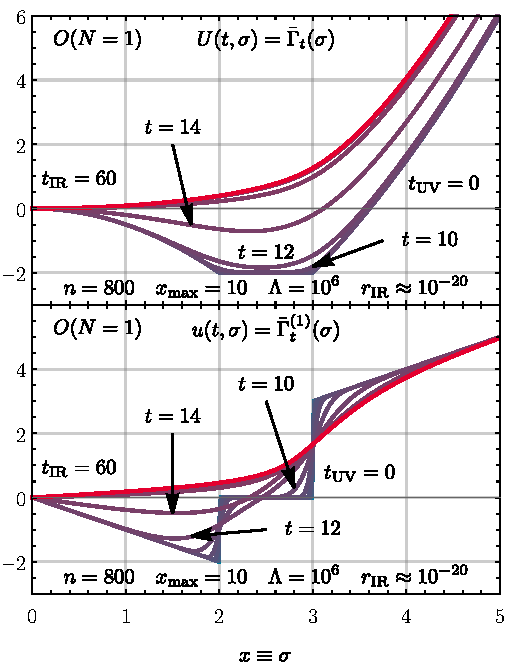
\includegraphics[width=\subcaptionFigureWidth]{0d/figures/sc_i_on=1_n=800_xmax=10_lambda=1.0e6_tir=60_rg_flow.pdf}
		\caption{\frg{} flow of the effective potential $U ( t , \sigma )$ (upper panel) and its derivative $u ( t , \sigma ) = \partial_\sigma U ( t , \sigma )$ (lower panel)}
		\label{fig:sc_i_on=1_n=800_xmax=10_lambda=1.0e6_tir=60_rg_flow}%
	}%
	{
		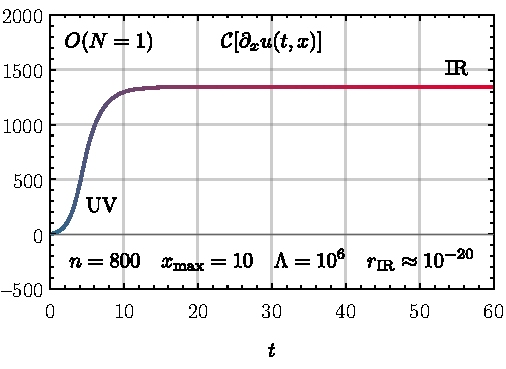
\includegraphics[width=\subcaptionFigureWidth]{0d/figures/sc_i_on=1_n=800_xmax=10_lambda=1.0e6_tir=60_entropy_flow.pdf}
		\caption{\frg{} flow of the numerical entropy $\mathcal{C} [ \partial_x u ( t, x ) ]$}%
		\label{fig:sc_i_on=1_n=800_xmax=10_lambda=1.0e6_tir=60_entropy_flow}%
	} % left figure
	{%
		\caption{
			\frg{} flow of the effective potential and its derivative on the top \subref{fig:sc_i_on=1_n=800_xmax=10_lambda=1.0e6_tir=60_rg_flow} and corresponding flow of the numerical entropy below  \subref{fig:sc_i_on=1_n=800_xmax=10_lambda=1.0e6_tir=60_entropy_flow} for the zero-dimensional \ONn{1} model with initial condition \cref{eq:testing_scenario_non-analytic_quadaratic_asymptote}.
			{Blue} color is associated to the \uv{} and {red} color to the \ir{}.
			We used the exponential regulator \cref{eq:exponential_regulator} with \uv{} scale $\Lambda = 10^6$.
			The lower panel in \subref{fig:sc_i_on=1_n=800_xmax=10_lambda=1.0e6_tir=60_rg_flow} is identical to the upper panel in \cref{fig:sc_i_on_1_10_100_n_800_xmax_10_lambda_1e6_tir_60_rg_flow}.
			\fromFigs{1 and 2}{zerod2}
		}\label{fig:sc_i_on=1_n=800_xmax=10_lambda=1.0e6_tir=60}
		\vspace{2cm}
	}%
\FloatBarrier
\paragraph{Test case I: Non-analytic initial condition}\phantomsection\label{paragraph:sc1O1}\mbox{}\\%
We begin our discussion of $O(1)$ models with test case I \eqref{eq:testing_scenario_non-analytic_quadaratic_asymptote}, recall \cref{fig:sc_i_uv_initial_condition} for a visualization of this \ic{}.
The \frg{} flow of $u ( t, x )$ for $N=1$ is presented in \cref{fig:sc_i_on=1_n=800_xmax=10_lambda=1.0e6_tir=60_rg_flow}.

The diffusive character of the \sigmaMode{} is clearly visible from the fact that it smoothens the discontinuities at $x = 2$ and $x = 3$, without any directed propagation (advection) of the conserved quantity $u ( t, x )$. 
Recall that the system has to restore the \ZII{} symmetry in the ground state as dictated the \cmwhTheoremWithRefs{}.
In particular, the potential has to become convex~\cite{Wipf:2013vp,Fujimoto:1982tc}.
This can be directly observed in the plot of the \frg{} flow and read off from \cref{tab:sc_o1_2_point_functions_exact} \dash{} the two-point function is positive at $\sigma = 0$.\bigskip
	
In \cref{fig:sc_i_on=1_n=800_xmax=10_lambda=1.0e6_tir=60_entropy_flow} we present the \frg{} flow of the (discretized numerical) entropy function for our first test case.

As expected from our discussion in \cref{subsubsec:0dO1entropy_c-function_tvd}, the entropy grows monotonically.
It increases by two orders of magnitude starting at zero in the \uv{} until it reaches (again) a plateau in the \ir{}.
We find that the entropy grows most when the regulator \eqref{eq:exponential_regulator} reaches the model scales.
Loosely speaking, this is where most of the dynamics takes place, see \cref{fig:sc_i_on=1_n=800_xmax=10_lambda=1.0e6_tir=60_rg_flow} (approximately between $t \approx 4$ and $t \approx 8$).
This is the \rgtime{} frame in which the diffusion smears out the discontinuities.
From a fluid- and thermodynamic perspective and directly on the level of the \pde{}, the whole process is intuitively understandable: Diffusion goes hand in hand with strong dissipation and a loss of information about the initial state of the system \dash{} the \uv{}, \cf{} \ccite{Zamolodchikov:1986gt,Zumbach:1994vg}.
This is directly comparable to heat conduction, where the information about the initial temperature distribution gets lost during the flow toward ``thermal'' equilibrium~\cite{Cannon:1984,LeVeque:1992,Lebowitz:2008} as discussed in our introduction of the linear \heq{} in \cref{subsec:hydroDiffusion}.

In the \frg{} framework, this translates to integrating out degrees of freedom from the \uv{} to the \ir{} and a growth in the number of coupling constants in $U ( t, \sigma )$, which is directly related to the growth of entropy.
The entropy plateau in the \ir{} is identified with the interacting \ir{} regime and an ``thermal'' equilibrium on the level of the diffusive \pde{}, whereas a plateau in the \uv{} is associated with a Gaussian \uv{} fixed point~\cite{Zinn-Justin:2010,ZinnJustin:2002ru}.
As expected the entropy stops changing at these points.
\ir{} solutions therefore correspond either to steady-flow solutions (in advection dominated systems for a large number of ``Goldstone'' modes~\cite{Nambu:1960tm,Goldstone:1961eq,Goldstone:1962es}) or to (thermal) equilibrium solutions (in diffusion dominated $O(1)$-symmetric systems) in the fluid-dynamical picture~\cite{Koenigstein:2021syz}.

Note that $t \in [ 0, 60 ]$ corresponds to an integration over $26$ orders of magnitude in $r(t)$, starting $6$ orders of magnitude above the model scales (which are of order one) and ending up $20$ orders of magnitude below the model scales. 
Interestingly, we find that the almost total absence of a plateau in the entropy in the \uv{} for our first test case implies that we almost violated \rgcy{}.
The absence of the zero-entropy plateau can also be seen by closer inspection of \cref{fig:sc_i_on_3_n_400_xmax_10_rir_10e-20_cutoff_test}, where $\Lambda = 10^6$ is barely on the plateau of \rgct{} \uv{} scales.

Before we continue with our next test case, we again note that the absolute value of $\mathcal{C} [\partial_x u ( t, x ) ]$ in the \ir{} in \cref{fig:sc_i_on=1_n=800_xmax=10_lambda=1.0e6_tir=60_entropy_flow} has no quantitative meaning, due to the ill-conditioned behavior when applied to the discontinuous initial condition \eqref{eq:testing_scenario_non-analytic_quadaratic_asymptote} of the numerical derivative \eqref{eq:centeredDifferences}. 
However, this does not spoil our qualitative arguments at all. 

\FloatBarrier
\fullWidthTwoColumnTwoSubFigures%
	[!t] % Placement
	{%
		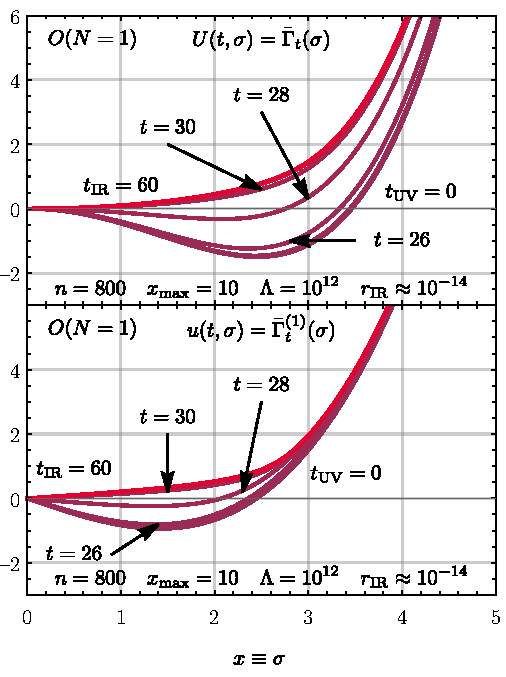
\includegraphics[width=\subcaptionFigureWidth-0.07cm]{0d/figures/sc_ii_n_on=1_n=800_xmax=10_lambda=1.0e12_tir=60_rg_flow.pdf}
		\caption{\frg{} flow of the effective potential $U ( t , \sigma )$ (upper panel) and its derivative $u ( t , \sigma ) = \partial_\sigma U ( t , \sigma )$ (lower panel)}
		\label{fig:sc_ii_n_on=1_n=800_xmax=10_lambda=1.0e12_tir=60_rg_flow}%
	}%
	{
		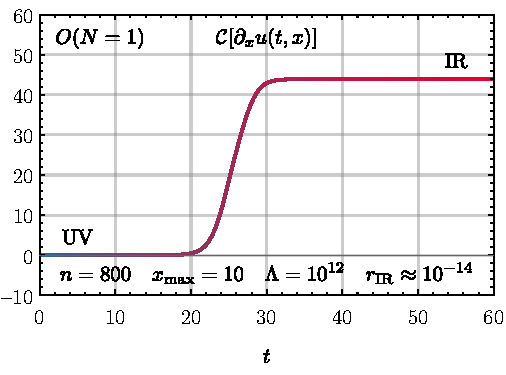
\includegraphics[width=\subcaptionFigureWidth]{0d/figures/sc_ii_n_on=1_n=800_xmax=10_lambda=1.0e12_tir=60_entropy_flow.pdf}
		\caption{\frg{} flow of the numerical entropy $\mathcal{C} [ \partial_x u ( t, x ) ]$}%
		\label{fig:sc_ii_n_on=1_n=800_xmax=10_lambda=1.0e12_tir=60_entropy_flow}%
	} % left figure
	{%
		\caption{
			\frg{} flow of the effective potential and its derivative on the top \subref{fig:sc_ii_n_on=1_n=800_xmax=10_lambda=1.0e12_tir=60_rg_flow} and corresponding flow of the numerical entropy below~\subref{fig:sc_ii_n_on=1_n=800_xmax=10_lambda=1.0e12_tir=60_entropy_flow} for the zero-dimensional $O(1)$ model with initial condition \eqref{eq:testing_scenario_phi4} with negative mass term.
			{Blue} color is associated to the \uv{} and {red} color to the \ir{}.
			We used the exponential regulator \cref{eq:exponential_regulator} with \uv{} scale $\Lambda = 10^{12}$.
			\fromFigs{3 and 5}{zerod2}
		}\label{fig:sc_ii_n_on=1_n=800_xmax=10_lambda=1.0e12_tir=60}
	}
	{\fullWidthTwoColumnFigureSpacing}
	{%
		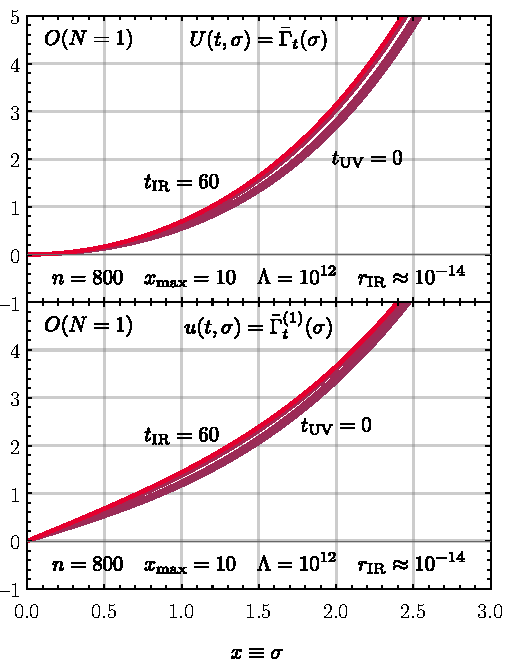
\includegraphics[width=\subcaptionFigureWidth]{0d/figures/sc_ii_p_on=1_n=800_xmax=10_lambda=1.0e12_tir=60_rg_flow.pdf}
		\caption{\frg{} flow of the effective potential $U ( t , \sigma )$ (upper panel) and its derivative $u ( t , \sigma ) = \partial_\sigma U ( t , \sigma )$ (lower panel).}
		\label{fig:sc_ii_p_on=1_n=800_xmax=10_lambda=1.0e12_tir=60_rg_flow}%
	}%
	{
		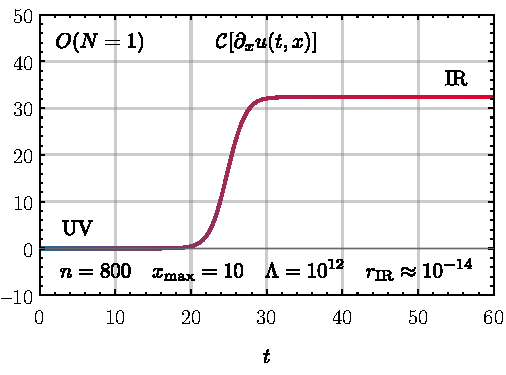
\includegraphics[width=\subcaptionFigureWidth-0.02cm]{0d/figures/sc_ii_p_on=1_n=800_xmax=10_lambda=1.0e12_tir=60_entropy_flow.pdf}
		\caption{\frg{} flow of the numerical entropy $\mathcal{C} [ \partial_x u ( t, x ) ]$}%
		\label{fig:sc_ii_p_on=1_n=800_xmax=10_lambda=1.0e12_tir=60_entropy_flow}%
	} % left figure
	{%
		\caption{
			\frg{} flow of the effective potential and its derivative on the top \subref{fig:sc_ii_p_on=1_n=800_xmax=10_lambda=1.0e12_tir=60_rg_flow} and corresponding flow of the numerical entropy below~\subref{fig:sc_ii_p_on=1_n=800_xmax=10_lambda=1.0e12_tir=60_entropy_flow} for the zero-dimensional $O(1)$ model with initial condition \eqref{eq:testing_scenario_phi4} with positive mass term.
			{Blue} color is associated to the \uv{} and {red} color to the \ir{}.
			We used the exponential regulator \cref{eq:exponential_regulator} with \uv{} scale $\Lambda = 10^{12}$.
			\fromFigs{4 and 6}{zerod2}
		}\label{fig:sc_ii_p_on=1_n=800_xmax=10_lambda=1.0e12_tir=60}
	}%
	[]\FloatBarrier
\paragraph{Test case II: \texorpdfstring{$\phi^4$}{phi**4} potential}\phantomsection\label{paragraph:sc2O1}\mbox{}\\%		
We continue our discussion of $O(1)$ models with test case II \eqref{eq:testing_scenario_phi4} with positive and negative mass term, recall \cref{fig:sc_ii_n_uv_initial_condition} for a visualization of this \ic{} with a negative mass term.
Depending on the sign of the mass term, we either start the \frg{} flow with a broken or restored \ZII{} symmetry.

When considering \cref{eq:testing_scenario_phi4} with negative mass term, we argued in \cref{paragraph:sc2taylorFlow} that during the \frg{} flow, while the physical point moves from $\sigma = \pm \sqrt{6}$ to $\sigma = 0$, presumably an excessively large or even infinitely many new couplings are generated in $U ( t, \sigma )$. 
This renders \frg{} Taylor expansion discussed in \cref{paragraph:sc2taylorFlow} at a finite order a potentially problematic approximation scheme for the evolution of non-convex potentials, see also \cref{subsubsec:sc3}.
In this paragraph, we reinforce our findings about the non-convergence of (Taylor) expansions of the potential during the \frg{} flow by studying the (numerical) entropy production during the \frg{} flows.

The \frg{} flows of $u ( t, x )$ for the \ic{} \eqref{eq:testing_scenario_phi4} with negative mass term is depicted in \cref{fig:sc_ii_n_on=1_n=800_xmax=10_lambda=1.0e12_tir=60_rg_flow} and \cref{fig:sc_ii_p_on=1_n=800_xmax=10_lambda=1.0e12_tir=60_rg_flow} shows the corresponding \frg{} flow\footnote{%
	Note that the plot range $x\in[0,3]$ for the ``positive mass''-case  differs from the one ($x\in[0,5]$) used in all other plots of \frg{} flows of $u ( t, x )$ in this subsubsection. 
	This is necessary to make the tiny changes during the \frg{} flow at least somewhat visible.
} for positive mass term.
Both \frg{} flows are by visual inspection not really spectacular: For the ``negative mass''-case, we find that, according to the \cmwhTheoremWithRefs{}, the diffusion via the \sigmaMode{} again restores the \ZII{} symmetry and drives the potential convex during the \rg{} flow before the system equilibrates in the \ir{}.
For the \frg{} flow of the ``positive mass''-case we only find minimal changes in the shape of $u ( t, x )$ also originating from the non-linear diffusion during the \frg{} flow.
Hence, the equilibrated solution in the \ir{} is relatively close to the \uv{} initial potential.\bigskip
	
The plots of the corresponding entropies in \cref{fig:sc_ii_n_on=1_n=800_xmax=10_lambda=1.0e12_tir=60_entropy_flow} (for negative mass term) and \cref{fig:sc_ii_p_on=1_n=800_xmax=10_lambda=1.0e12_tir=60_entropy_flow} (for positive mass term) are more instructive.
In both cases we find a clear monotonic rise of the (numerical) entropy exactly in the \frg{} time period, in which most of the dynamics takes place.
Furthermore, we clearly find plateaus in the \uv{} and the \ir{}, which correspond to the trivial \uv{} regime and the non-trivial interacting \ir{} regime.
This plateau-like behavior signals \rgcy{}.
In comparison with our first test case \eqref{eq:testing_scenario_non-analytic_quadaratic_asymptote}, where we used exactly the same discretization points (volume cells), the monotonic growth of entropy is less drastic and significantly smaller.
This is expected because the jumps in $u ( t = 0, x )$ at $x = 2$ and $x = 3$ in the first test case \eqref{eq:testing_scenario_non-analytic_quadaratic_asymptote} lead to greater changes in the discrete total variation \dash{} the arc length in $x$ of $u ( t, x )$ \dash{} than the rather small changes of the profiles of $u ( t, x )$ for the $\phi^4$-models, \cf{} \cref{paragraph:discrete_c_and_tvd}. 
Also from a fluid-dynamic perspective, this is intuitively understandable because the smoothening of huge gradients is a substantial source of entropy and obviously an irreversible process, whereas only a small transport of a fluid is not a source of excessive but rather small entropy production, even though it is diffusion driven.
Still, also for both $\phi^4$-cases the entropy increases during the \frg{} flow, which first signals an increasing number of coupling constants generated during the \frg{} flow, and second also renders the flows irreversible.
	
The second observation has severe consequences: Any \frg{} flow in a \frg{} Taylor expansion employs a finite set of coupled \odes{} for the couplings (vertices).
Since the system is finite, it seems to be theoretically possible integrate in either \rgtime{}-direction. 
In higher dimensions, one can formally integrate to larger scales when considering the perturbative beta functions of \qcd{}, \qed{}, \etc{}~\cite{Politzer:1973fx,Gross:1973id,Gross:1973ju,Gross:1974cs}, \cf{} \cref{paragraph:qcdAS}.
However, this is in principle not compatible with the irreversibility of \grg{} flows as shown in our present work (as, \eg{}, signaled by the rise of entropy)  and may only be reliable within small subspaces of the theory space associated with a given theory.
In fact, the computation of fundamental couplings at small scales (high energies) from effective couplings at large scales (low energies) is in general not possible, \cf{}\ \ccite{Wilson:1979qg}. We conclude that the increase of entropy, which we also observe during the \frg{} flow of our analytic initial conditions \eqref{eq:testing_scenario_phi4} reveals potential limitations of Taylor expansion of effective actions because most likely an extremely large (or even infinite) number of couplings is generated in the \frg{} flow and would be required to correctly describe the \frg{} flow 
\footnote{%
	At this point, one might be tempted to apply our definition of the normalized (numerical) entropy directly to some $\partial_x u ( t, x )$ that is reconstructed from the flow of the coefficients of a Taylor expansion of the potential to study the validity of the expansion.
	However, this is not possible, because the \frg{} Taylor expansion in general provides only an adequate local description of the potential, while our (numerical) entropy or the \tv{} requires knowledge about the global shape of the potential or its derivatives.
}.%

When considering an expansion in vertices (especially in higher/non-zero dimensions), it might be possible that higher-order couplings/vertices are strongly suppressed (especially when considering higher-dimensional \qfts{}), 
such that an expansion of the \frgEquation{} in vertices is applicable and meaningful in practice, see, \eg{}, \ccite{Eser:2018jqo,Eser:2019pvd,Divotgey:2019xea,Cichutek:2020bli}.
This should go hand in hand with only a small growth of an entropy for the exact \frg{} flow.
Exactly this seems to be the case for our ``positive mass'' case \eqref{eq:testing_scenario_phi4}, which shows almost no dynamics at all and yields the smallest increase in entropy of all our test cases. 
A reason, why here a rather small number of couplings might be sufficient to describe the entire \frg{} flow is that the potential is convex during the entire flow and has a single unique non-moving minimum.
Hence, the \uv{} regime of this model and the \ir{} regime do not differ much and, as long as the quartic coupling is extremely small, also perturbation theory~\cite{Strocchi:2013awa} leads to results which are consistent with the exact values for the lowest \ipi{} \nptFunctions{}~\cite{Keitel:2011pn}.

\fullWidthTwoColumnTwoSubFigures{%
		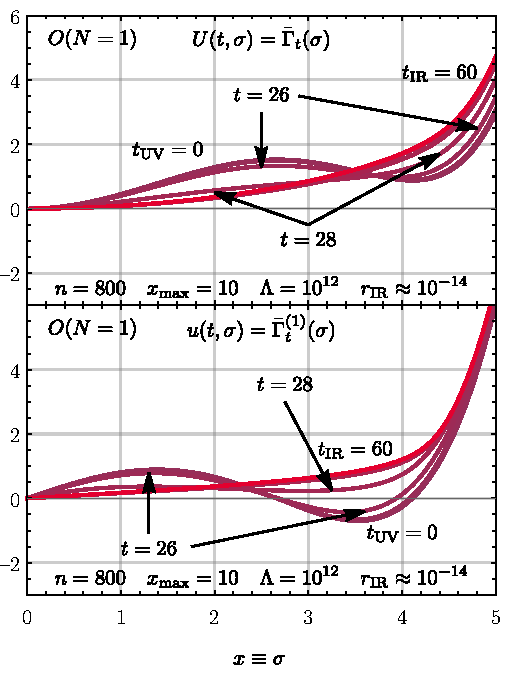
\includegraphics[width=\subcaptionFigureWidth-0.015cm]{0d/figures/sc_iii_on=1_n=800_xmax=10_lambda=1.0e12_tir=60_rg_flow.pdf}
		\caption{\frg{} flow of the effective potential $U ( t , \sigma )$ (upper panel) and its derivative $u ( t , \sigma ) = \partial_\sigma U ( t , \sigma )$ (lower panel).}
		\label{fig:sc_iii_on=1_n=800_xmax=10_lambda=1.0e12_tir=60_rg_flow}%
	}%
	{
		\vspace{-0.01cm}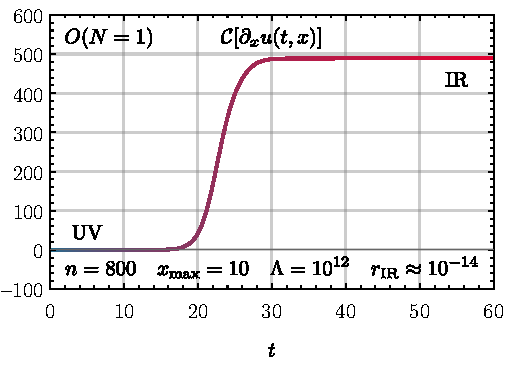
\includegraphics[width=\subcaptionFigureWidth]{0d/figures/sc_iii_on=1_n=800_xmax=10_lambda=1.0e12_tir=60_entropy_flow.pdf}
		\caption{\frg{} flow of the numerical entropy $\mathcal{C} [ \partial_x u ( t, x ) ]$}%
		\label{fig:sc_iii_on=1_n=800_xmax=10_lambda=1.0e12_tir=60_entropy_flow}%
	} % left figure
	{%
		\caption{
			\frg{} flow of the effective potential and its derivative on the top \subref{fig:sc_iii_on=1_n=800_xmax=10_lambda=1.0e12_tir=60_rg_flow} and corresponding flow of the numerical entropy below~\subref{fig:sc_iii_on=1_n=800_xmax=10_lambda=1.0e12_tir=60_entropy_flow} for the zero-dimensional $O(1)$ model with initial condition \eqref{eq:testing_scenario_phi6}.
			{Blue} color is associated to the \uv{} and {red} color to the \ir{}.
			We used the exponential regulator \cref{eq:exponential_regulator} with \uv{} scale $\Lambda = 10^{12}$.
			\fromFigs{7 and 8}{zerod2}
		}\label{fig:sc_iii_on=1_n=800_xmax=10_lambda=1.0e12_tir=60}
	}%
	{\fullWidthTwoColumnFigureSpacing}%
	{%
		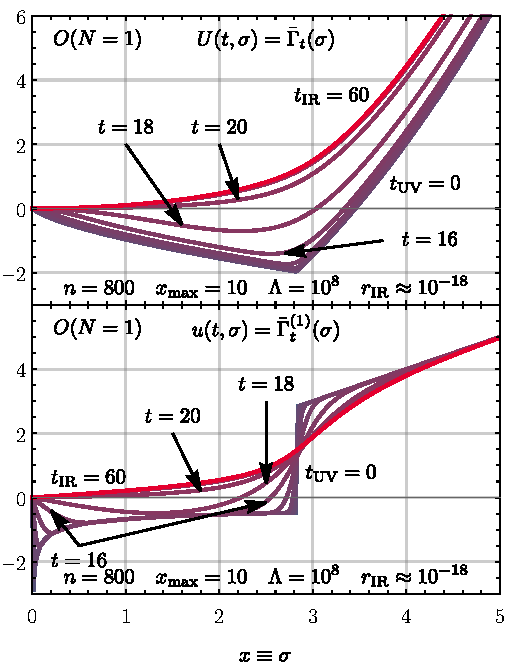
\includegraphics[width=\subcaptionFigureWidth]{0d/figures/sc_iv_on=1_n=800_xmax=10_lambda=1.0e8_tir=60_rg_flow.pdf}
		\caption{\frg{} flow of the effective potential $U ( t , \sigma )$ (upper panel) and its derivative $u ( t , \sigma ) = \partial_\sigma U ( t , \sigma )$ (lower panel).}
		\label{fig:sc_iv_on=1_n=800_xmax=10_lambda=1.0e8_tir=60_rg_flow}%
	}%
	{
		\vspace{0.05cm}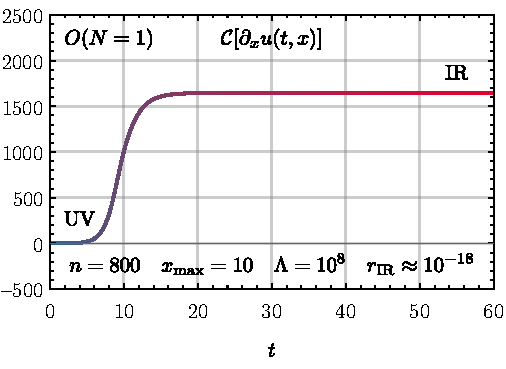
\includegraphics[width=\subcaptionFigureWidth-0.01cm]{0d/figures/sc_iv_on=1_n=800_xmax=10_lambda=1.0e8_tir=60_entropy_flow.pdf}
		\caption{\frg{} flow of the numerical entropy $\mathcal{C} [ \partial_x u ( t, x ) ]$}%
		\label{fig:sc_iv_on=1_n=800_xmax=10_lambda=1.0e8_tir=60_entropy_flow}%
	} % left figure
	{%
		\caption{
			\frg{} flow of the effective potential and its derivative on the top \subref{fig:sc_iv_on=1_n=800_xmax=10_lambda=1.0e8_tir=60_rg_flow} and corresponding flow of the numerical entropy below~\subref{fig:sc_iv_on=1_n=800_xmax=10_lambda=1.0e8_tir=60_entropy_flow} for the zero-dimensional $O(1)$ model with initial condition \eqref{eq:testing_scenario_4}.
			{Blue} color is associated to the \uv{} and {red} color to the \ir{}.
			We used the exponential regulator \cref{eq:exponential_regulator} with \uv{} scale $\Lambda = 10^8$.
			\fromFigs{9 and 10}{zerod2}
		}\label{fig:sc_iv_on=1_n=800_xmax=10_lambda=1.0e8_tir=60}
	}%
	[]
\FloatBarrier
\paragraph{Test case III: \texorpdfstring{$\phi^6$}{phi**6} potential}\phantomsection\label{paragraph:sc3O1}\mbox{}\\%		 
We continue our discussion of $O(1)$ models with test case III \eqref{eq:testing_scenario_phi6}, recall \cref{fig:sc_iii_uv_initial_condition} for a visualization of this \ic{}.
In \cref{paragraph:sc3taylorConclusion}, we came to the conclusion that there has to be a time interval during the \frg{} flow, where $u ( t, x )$ exhibits highly non-local dynamics \dash{} preventing the applicability of a Taylor expansion, even though the expansion point is unique and does not move.
The \frg{} flows of $u ( t, x )$ for \eqref{eq:testing_scenario_phi6} with negative mass term is depicted in \cref{fig:sc_iii_on=1_n=800_xmax=10_lambda=1.0e12_tir=60_rg_flow}.

At $t \approx 27$ the local minimum (the second non-trivial zero-crossing) vaporizes via the diffusion and merges with the local maximum.
It is this dynamics which triggers the breakdown of the Taylor expansion manifesting as strongly oscillating and ultimately diverging couplings at $t \approx 27$. \bigskip

Interestingly, also the (numerical) entropy function signals exactly the discussed non-local behavior at $t \approx 27$.
At that point in time, when the local minimum vaporizes, we observe the strongest increase of entropy, see \cref{fig:sc_iii_on=1_n=800_xmax=10_lambda=1.0e12_tir=60_entropy_flow}.
We also find that by absolute measures, the entropy production for the $\phi^6$-initial potential \eqref{eq:testing_scenario_phi6} is greater than the entropy production observed for both quartic initial conditions~\eqref{eq:testing_scenario_phi4}.
Nevertheless, the entropy production for the non-analytic initial condition~\eqref{eq:testing_scenario_non-analytic_quadaratic_asymptote} is still greater than the one in the $\phi^6$-case.
This can be understood from the relation of the numerical entropy to the \tv{}, \ie{}, the arc length of $u ( t, x )$ which even formally diverges for \cref{eq:testing_scenario_non-analytic_quadaratic_asymptote} in the \uv{}, keeping in mind that a comparison of absolute values of the numerical entropy should be considered with some care, \cf{} \cref{paragraph:discrete_c_and_tvd}.
	
We conclude this paragraph noting that that the (numerical) entropy might be a useful measure for deciding whether a system at a given \rgscale{}/time is in a perturbative or non-perturbative regime.
In other words, it is a tool to discuss whether the \frg{} flow is governed by strong (non-perturbative) dynamics or by weak (perturbative) dynamics.
The \cfd{} analogy to this situation would be the difference between a fluid evolving through an out-of-equilibrium state, before finally equilibrating or showing steady-flow behavior, in contrast to a fluid that is already close to its equilibrium state.

\paragraph{Test case IV: The \texorpdfstring{$\sigma = 0$}{sigma=0} boundary}\phantomsection\label{paragraph:sc4O1}\mbox{}\\%
We conclude our discussion of explicit numerical results for the $O(1)$ model with test case IV~\eqref{eq:testing_scenario_4}, recall \cref{fig:sc_iv_uv_initial_condition} for a visualization of this \ic{}.
The test case~\eqref{eq:testing_scenario_4} turns out to be a highly interesting almost pathological example in this context.
The \frg{} flow of $u ( t, x )$ is shown in \cref{fig:sc_iv_on=1_n=800_xmax=10_lambda=1.0e8_tir=60_rg_flow}.

Of specific interest regarding the (numeric) entropy is of course the pole of $u ( t = 0, x )$ at $x = 0$.
Formally, the arc length of $u ( t, x )$, which is directly related to our entropy function, diverges due to the pole at $x = 0$ for all $t > 0$.
This divergence is of different nature than the divergence caused by integrating from $x = - \infty$ to $x = + \infty$ in \cref{eq:entropy_func}.
Whereas the latter can be cured by normalizing the entropy \wrt{} the entropy of $u ( t = 0, x)$, the present divergence also occurs on the level of the ``normalized''  entropy function \eqref{eq:Cdef} similar to the other non-analytic jumps in the \uv{}.
The reason for the infinite entropy production while going from $t = 0$ to $t > 0$ is exactly that the total variation between $- x_{\mathrm{max}}$ and $+ x_{\mathrm{max}}$ turns finite for $u ( t, x )$ during the flow because the potential turns convex and smooth.
Moreover, symmetry restoration in the ground state sets in for $t \rightarrow \infty$.
However, it is still normalized against the infinite total variation of $u ( t = 0, x )$.
Interestingly, this problem can be traced back to the initialization of the \frg{} flow equations at $t = 0$ with the classical \uv{} action $\bar{\Gamma}_{t = 0} ( \varphi ) = \mathcal{S} ( \varphi )$, which is actually not totally exact but rather an almost perfect approximation for sufficiently large $\Lambda$, see also our discussion in \cref{subsubsec:zerodICS}.
However both the inherent diffusive nature of the \frg{} flow equation and the employed finite-volume discretization render the pole at $\sigma = 0$ a huge but already finite jump captured in three volume cells on the level of the cell averages $\bar{u}_i ( t )$ at $t = 0$.
Therefore, we can use $u ( t = 0, x )$ as our reference entropy for the normalization of \cref{eq:Cdef} as it is numerically finite right from the beginning of the flow.\bigskip

The explicit result for the \frg{} flow of our (numerical) entropy is shown in \cref{fig:sc_iv_on=1_n=800_xmax=10_lambda=1.0e8_tir=60_entropy_flow}.
Irrespective of the subtleties of the preceding discussion, we find a rather large entropy production at exactly those times when the pole vanishes and the jumps at $x = \pm \sqrt{8}$ are smeared out via the diffusion.

Additionally, we find that the total entropy production is much larger for this test case than for the previous ones. Again, this is of course directly related to the huge gradients in the initial condition, which are tremendous sources of entropy via dissipation, directly analogous to the \he{} discussed in \cref{paragraph:HE}.\bigskip

In this subsubsection, we confronted our theoretical findings of \cref{subsubsec:0dO1entropy_c-function_tvd} with direct numerical computations using the \ktScheme{}.
We verified the behavior of the function $\mathcal{C} [ \partial_x u ( t, x ) ]$ from \cref{eq:Cdef} by means of its discretized version in \cref{eq:Cdiscrete} as a valid numerical entropy measure in four test cases.
Using the numerical entropy and the Wetterich equation in the form~\eqref{eq:o(1)_wetterich_equation}, we made several, at this point almost intuitive, connections between phenomena known in fluid- and thermodynamic processes and directly related processes and aspects of \grg{} flows.
Most notable, the diffusive character of the flow equation~\eqref{eq:o(1)_wetterich_equation} results directly in irreversible \frg{} flows.
This also establishes a connection between steady-state/(thermal) equilibrium solutions and the \uv{}  and \ir{} regime.
Moreover, the application of the numerical entropy and total variation appears to be an attractive monitor for \rgcy{} and the origin of an ``thermodynamic'' time asymmetry.

\subsubsection{Irreversibility of the RG flow, entropy, and the \texorpdfstring{$\mathcal{C}$}{C}-theorem}
\label{subsubsec:c-theorem_irreversibility_entropy}
\begin{disclaimer}
	This subsubsection summarizes and references the findings of Sec. V of \ccite{Koenigstein:2021rxj}.
	The \customref{paragraph:cTheoremzerodO1}{first paragraph} of this subsubsection includes material for the Virasoro algebra and fixed-point solutions for the zero-dimensional \ONn{1} from the unpublished notes~\cite{Koenigstein:fixedPoint}.
\end{disclaimer}
The (re)discoveries within this work unravel the connection between the (numerical) entropy and total variation, employed in applied mathematics, and the irreversibility inherent to \grg{} flows. Furthermore, they might even provide some connections to $\mathcal{C}$-/$\mathcal{A}$-theorems within the framework of truncated \frg{} flow equations. 

The original formulation of Zamolodchikov's $\mathcal{C}$-theorem~\cite{Zamolodchikov:1986gt} states that for a two-dimensional field theory the following properties hold:
\begin{enumerate}
	\item There exists a positive function 
		\begin{align}
			\mathcal{C} ( \{ g_i \}, t ) \geq 0 \, ,	\label{eq:c-function_1}
		\end{align}
	of all (possibly infinitely many) dimensionless couplings $\{ g_i \}$ of the theory and \rgtime{} $t$, with the additional property
		\begin{align}
			+\dod{}{t} \mathcal{C} ( \{ g_i \}, t ) \geq 0 \, ,	\label{eq:c-function_2}
		\end{align}
	where the choice of sign in front of the derivative is convention.
	
	\item The $\mathcal{C}$-function takes a fixed value at (critical) fixed points $g_i^\ast$ of the theory:
		\begin{align}
			\mathcal{C} ( \{ g_i^\ast \}, t ) = c_i \, ,	\label{eq:c-function_3}
		\end{align}
	where the fixed value $c_i$ can be identified with the central charge $c$ (giving  the $\mathcal{C}$-theorem its name) of a \textit{Virasoro algebra}~\cite{Virasoro:1969zu}
		\begin{align}
			\big[ L_m, \, L_n \big] = L_m L_n - L_n L_m = \,& ( m - n ) \, L_{m + n} + \frac{c}{12} \, ( m^3 - m ) \, \delta_{m + n, 0} \, ,	\label{eq:c-function_virasoro}
		\end{align}
	with the generators $L_n$ of the infinite conformal group.
	The central charge is different for different fixed points.
\end{enumerate}
$\mathcal{C}$-theorems and their generalizations especially from two to four dimensions $\mathcal{A}$-theorems~\cite{Cardy:1988cwa} are still under active research, see, \eg{}, \ccite{Zamolodchikov:1986gt,Rosten:2010vm,Banks:1987qs,Cardy:1988cwa,Osborn:1989td,Jack:1990eb,Komargodski:2011vj,Curtright:2011qg,Haagensen:1993by,Generowicz:1997he,Forte:1998dx,Codello:2013iqa,Codello:2015ana,Becker:2014pea,Becker:2016zcn}.
$\mathcal{A}$-theorems get their name from anomaly coefficients which are proposed to take the role of the central charge in four dimensions.
A general overview of this field is beyond the scope of the current work and we will focus in the following paragraphs on specific aspects relevant to this work and the \frg{}.

One other interesting aspect, related to the introduction of a numeric entropy for \frg{} flows, was pointed out by the referee of \ccite{zerod2}: the present formulation based on the effective potential shares some similarities with the macroscopic description of systems in statistical mechanics.
Instead of working with an infinite set of couplings (microstates in statistical mechanics) we switch to a description in terms of an effective potential (a macroscopic formulation in statistical mechanics).
The inability (of a macroscopic observer) to track the dynamics of an infinite set of couplings (microstates in statistical mechanics) leads to a macroscopic entropy production/information loss and irreversible processes.
An approach to formalize this notion in statistical mechanics was made by Ludwig Boltzmann~\cite{Boltzmann2003} and later Josiah W. Gibbs~\cite{Gibbs2010Sep} with the introduction of $H$-theorems, see, \eg{}, Chap. VI and XII of the textbook~\cite{Tolman1979Nov} for further details. Exploring this connection and possible relations between  $\mathcal{C}$-/$\mathcal{A}$- and $H$-theorems further could be a very interesting prospect for further research.

\paragraph{The \texorpdfstring{$\mathcal{C}$}{C}-theorem of the zero-dimensional \texorpdfstring{\ONn{1}}{O(1)} model}\phantomsection\label{paragraph:cTheoremzerodO1}\mbox{}\\%
In this paragraph we will argue that our numerical entropy \eqref{eq:Cdef} for the zero-dimensional \ONn{1} model is in fact a direct analogon to Zamolodchikov's $\mathcal{C}$-function in zero dimensions.
Our numerical entropy \eqref{eq:Cdef} fulfills the first two defining properties \eqref{eq:c-function_1} and \eqref{eq:c-function_2} by construction.
$\mathcal{C} [ \partial_x u ( t, x ) ]$ and its \fv{} equivalent $\mathcal{C} [ \{\bar{u}_j(t)\}]$ are also functions of all (infinitely many) coupling constants which are dimensionless in ${d=0}$ and encoded via $u ( t, x )$ or equivalently in \fv{} discretization in the set of volume averages $\{\bar{u}_j(t)\}$.

The only open question regarding the interpretation of our numerical entropy \eqref{eq:Cdef} as a $\mathcal{C}$-theorem is related to the question of fixed points and the central charge.
\Apriori{} it is difficult to just imagine a meaningful zero-dimensional analog of central charge and conformal symmetry.
\Aposteriori{} \dash{} after an extensive review of the literature of zero-dimensional \qfts{} and specifically zero-dimensional \ON{} models \dash{} there might be a meaningful analogon for the central charge, \ie{}, the absence of such charges, in zero dimension.
S. Nishigaki and T. Yoneya in \ccite{Nishigaki:1990sk}  and P. Di Vecchia, M. Kato, and N. Ohta in \ccite{DiVecchia:1990ce} observe, that it is possible to derive \dses{} for the zero-dimensional $O(N)$ model which can be recast into a Virasoro algebra.
Following \ccite{Nishigaki:1990sk} we consider the partition function $\mathcal{Z}$ as a function of all, infinitely many couplings $\{\lambda_j\}$ of a zero-dimensional \ON{} model
\begin{align}
	\mathcal{Z} ( \{\lambda_j\} ) \equiv \int \dif^{\,N}\! \phi \, \exp \bigg[ - \sum_{j = 1}^{\infty} \lambda_j \, ( \vec{\phi}^{\, 2} \, )^j \bigg]\,.\label{eq:zerodO1Zdse}
\end{align}
From the divergence theorem, we find for $n \in \Integers{}_0$
\begin{align}
	0 = \, & \int \dif^{\,N}\! \phi \, \frac{\partial}{\partial \phi^i} \bigg( \phi^i \, ( \vec{\phi}^{\, 2} )^n \, \exp \bigg[ - \sum_{j = 1}^{\infty} \lambda_j \, ( \vec{\phi}^{\, 2} \, )^j \bigg] \bigg)\, ,
\end{align}
%For $n = 0$, we find
	%\begin{align}
		%0 = \, & \bigg( \tfrac{N}{2} + \sum_{j = 1}^{\infty} j \, \lambda_j \, \frac{\partial}{\partial \lambda_j} \bigg) \, \mathcal{Z} ( \vec{\lambda} \, ) \, ,
	%\end{align}
%while for $n \geq 1$
	%\begin{align}
		%0 = \, & \bigg[ - \big( \tfrac{N}{2} + n \big) \, \frac{\partial}{\partial \lambda_n} + \sum_{j = 1}^{\infty} j \, \lambda_j \, \frac{\partial}{\partial \lambda_{j + n}} \bigg] \, \mathcal{Z} ( \vec{\lambda} \, ) \, ,
	%\end{align}
%where we additionally divided by a factor of two.
which when evaluated for $n=0$ and $n \geq 1$ allow for the definition of 
\begin{align}
	L_n \equiv \, & - \big( \tfrac{N}{2} + n \big) \, \frac{\partial}{\partial \lambda_n} + \sum_{j = 1}^{\infty} j \, \lambda_j \, \frac{\partial}{\partial \lambda_{j + n}} \label{eq:zerodO1L}
\end{align}
such that
\begin{align}
	0 = L_n \, \mathcal{Z} ( \{\lambda_j\} ) \, .\label{eq:zerodO1dse}
\end{align}
These operators $L_n$ form an algebra
\begin{align}
	\big[ L_m, \, L_n \big] = \, & ( m - n ) \bigg[ - \big( \tfrac{N}{2} + m \big) \, \frac{\partial}{\partial \lambda_{m + n}} +  \sum_{i = 1}^{\infty} i \, \lambda_i \, \frac{\partial}{\partial \lambda_{i + m + n}} \bigg] = \, ( m - n ) \, L_{m + n} \, ,\label{eq:c-function_witt}
\end{align}
which is a Virasoro algebra \eqref{eq:c-function_virasoro} with vanishing central charge $c$, \ie{}, a so-called \textit{Witt algebra}~\cite{Witt1937Jan}.
The \dses{} \eqref{eq:zerodO1dse} for $\mathcal{Z} ( \{\lambda_j\} )$ inform and establish the Witt algebra \eqref{eq:c-function_witt}, \ie{}, a Virasoro algebra with vanishing central charge, for the zero-dimensional \ON{} model.
Following Zamolodchikov and assuming that the operators for the \dses{} $L_n$ from \cref{eq:zerodO1L} are a meaningful zero-dimensional analogon to the generators $L_n$ of the infinite conformal group in two dimensions, one would assume that \cref{eq:c-function_witt} implies an absence of fixed-point solutions in zero-dimensional \ON{} models.

We will prove the latter for the zero-dimensional \ONn{1} model explicitly.
We start from the \frg{} flow equation \eqref{eq:o(1)_wetterich_equation} by reformulating the equation at finite \rgtime{} in terms of the regulator itself
\begin{align}
	\partial_r u ( r, x ) = \frac{1}{2} \, \dod{}{x} \frac{1}{r + \partial_x u ( r , x )} \, ,
\end{align}
which in turn may be rewritten using the substitution $u ( r, x ) \equiv w ( r, x ) - r \, x$:
\begin{align}
	\partial_r w ( r, x ) - x = \, & \frac{1}{2} \, \dod{}{x} \frac{1}{\partial_x w( r , x )}\, .
\end{align}
Hence, the global fixed-point equation (with $\partial_r w ( r, x )=0$) reads
\begin{align}
	- x = \frac{1}{2} \, \dod{}{x} \frac{1}{\partial_x w ( r , x )}\,,
\end{align}
which can be integrated to
\begin{align}
	x_0^2 - x^2 = \frac{1}{\partial_x w ( r, x )} - \frac{1}{\partial_{x_0} w ( r, x_0 )}
\end{align}
The potential $U ( r, x )$ has to be \ZII{}-symmetric and convex for all $r$, if it is supposed to be an admissible global fixed-point solution.
Thus, $\partial_x w ( r, x )$ has to be positive for all $x_0 \neq 0$. 
As long as we choose $x_0 \in ( 0, \pm \infty )$, explicitly excluding $x_0 = 0$ and $x_0 = \pm \infty$, we can absorb both integration constants in a non-zero, positive integration constant, which we set \wlogA{} to unity in the following, and derive
\begin{align}
	\partial_x w ( r, x ) = \frac{1}{1 - x^2} \, .
\end{align}
This equation can be integrated to obtain
\begin{align}
	w ( r, x ) =
	\begin{cases}
		\mathrm{artanh} ( x ) \, ,	&	|x| < 1 \, ,
		\\
		\mathrm{arcoth} ( x ) \, ,	&	|x| > 1 \, ,
	\end{cases}\label{eq:zerodO1w}
\end{align}
which however implies, that there is only a convex solution to the fixed-point equation for $x \in ( - 1, + 1)$. 
In conclusion, a global convex fixed-point solution does not exist.
We may also note that the partition function \eqref{eq:partition_function} for the potential $U ( r, x ) = W ( r, x ) - \frac{1}{2} \, r \, x^2$ with the integral of \cref{eq:zerodO1w} does not converge since $\lim_{x\rightarrow \pm\infty}W(r,x)=1+\frac{1}{2}\ln(x^2)+\order(x^{-2})$.\bigskip

In summary we note that our numerical entropy \eqref{eq:Cdef} for the zero-dimensional \ONn{1} model is a proper analogon to  Zamolodchikov's $\mathcal{C}$-function. The following $\mathcal{C}$-theorem holds for the zero-dimensional \ONn{1} model: $\mathcal{C} [ \partial_x u ( t, x ) ]$ from \cref{eq:Cdef} and its discrete \fv{} equivalent $\mathcal{C} [ \{\bar{u}_j(t)\}]$ from \cref{eq:Cdiscrete} are positive and monotonically increasing during \frg{} flow and there are no global, convex fixed-point solutions with the Witt algebra~\eqref{eq:c-function_witt} for the \dses{}~\eqref{eq:zerodO1dse} as analogon to the Virasoro algebra~\eqref{eq:c-function_virasoro}.

\paragraph{The challenges of a generalization to finite $N>1$ in zero dimensions}\phantomsection\label{paragraph:cTheoremzerodON}\mbox{}\\%
To discuss the construction of a $\mathcal{C}$-function for $N>1$ we recall the \frg{} flow \cref{eq:advection_diffusion_equation_zero-dimensional} 
\begin{align}
	&\partial_t u + \dod{}{x} F [ t, x, u ] = \dod{}{x} Q [ t, \partial_x u ]\, ,
\end{align}
and its primitive form
\vspace{-.05em}
\begin{align}
&\partial_t u + \frac{\partial F [ t, x, u ]}{\partial u}  \, \partial_x u - \frac{\partial Q [ t, \partial_x u ]}{\partial(\partial_x u)} \partial_x^2 u ( t, x ) = -\partial_x F [ t, x, u ]\,.\label{eq:zerodO1primitive}
\end{align}
\vspace{-.05em}
\Cref{eq:zerodO1primitive} includes convective contributions on the \lhs{} but also an internal source term, stemming from the position-dependence of the advection flux, on the \rhs{}
We discussed such a situation in the general \cfd{} context in \cref{subsec:hydroAdvection} and implications for the \tv{} in \cref{subsec:hydroKT}: (internal) source terms lead to a loss of the \tvni{} property \dash{} they change and crucially increase \tv{}/arc length during time evolution.
Hence \tv{} is no longer a valid candidate for a numerical entropy functional, which in presence of sources is notoriously difficult to construct in a \cfd{} context, see, \eg{}, \ccite{Monthe:2001,Beneito2008,Chen2011May,Bessemoulin:2012} and references therein. 

The explicit position-dependence of the advection flux prevented us from formulating a numerical entropy for the zero-dimensional $O(N)$ model for finite $N > 1$.
The corresponding contribution to the entropy function \eqref{eq:Cdef} allows for $\tfrac{\dif}{\dif t} \, \mathcal{C} [ \partial_x u ( t, x ) ] < 0$ during \frg{} flow for certain initial conditions and $N$ in the case of $N > 1$.
For the zero-dimensional cases \eqref{eq:testing_scenario_phi4} and \eqref{eq:testing_scenario_phi6} discussed, we find $\tfrac{\dif}{\dif t} \, \mathcal{C} [ \partial_x u ( t, x ) ] < 0$ during the \rg{} evolutions for $N \geq 8$.
For the cases \eqref{eq:testing_scenario_non-analytic_quadaratic_asymptote} and \eqref{eq:testing_scenario_4} with their $\sigma^2$ asymptotics for large $\sigma$ the inequality $\tfrac{\dif}{\dif t} \, \mathcal{C} [ \partial_x u ( t, x ) ] \geq 0$ seems to hold for all $N$ and $t$.

Reformulating the \frg{} flow \cref{eq:conservation_law_u_phi} in the invariant $y\equiv \tfrac{1}{2} \, x^2$, \cf{} \cref{eq:conservation_law_u_rho}, does not solve the issue of internal source terms at finite $N$. 
While the advection flux in \cref{eq:conservation_law_u_rho} loses its explicit position-dependence the diffusion flux gains both a dependence on $u(t,y)$ and $y$ which does not improve our situation at finite $N$.
In the infinite-$N$ limit however diffusive contributions vanish after rescaling with $N-1$ and a formulation in $y$ with a $y$-independent advection flux allows for an identification of the \tv{} as an entropy functional.
We will discuss this in \cref{paragraph:infiniteNflowsEntropy}.

\vspace{-.65em}
\paragraph{Comments on a generalization to (higher-dimensional) \texorpdfstring{$O(N)$}{O(N)} models}\phantomsection\label{paragraph:cTheoremON}\mbox{}\\
A direct generalization of our findings regarding numerical entropy measures for the \frg{} flow from zero to non-zero dimensions is hindered by two new conceptual issues:
\begin{enumerate}
	\item The \lpa{} as part of the leading-order of a \de{} is in general only a truncation in $d>0$, \cf{} \deRef{}.
	This makes very general statements for the \qft{} under consideration \apriori{} impossible when just discussing the \frg{} flow of the potential.
	That being said the established concept of numerical entropy might still be of some use in higher-dimensional $O(1)$ models.
	\item	In contrast to the zero-dimensional model, the couplings in $d>0$ can have non-zero energy dimensions.
	Thus, our numerical entropy \eqref{eq:Cdef} cannot adequately describe the second property of the $\mathcal{C}$-theorem \eqref{eq:c-function_3} \dash{} namely capturing the properties of fixed points, which are defined via the zeroes of the beta functions of all dimensionless couplings and additionally a constant $\mathcal{C}$-/$\mathcal{A}$-function.
	To resolve the fixed-point structure, one has to consider the flow equation for rescaled quantities which gains additional internal source terms due to the rescaling, \cf{} Eq. (37) of \ccite{zerod2}.
	Such source terms make \tv-like entropy measures unviable.
\end{enumerate}
Further details can be found in Sec. V of \ccite{zerod2}.\clearpage

\FloatBarrier
\subsection{The \ON{} model in the large-\texorpdfstring{$N$}{N} limit}\label{subsec:0dLargeN}
\begin{disclaimer}
	This subsection is based on \ccite{Steil:2021cbu}.
	The plots of \ccite{Steil:2021cbu} and the underlying numerical data were produced by myself and numerically cross-checked by A. Koenigstein.
	
	The plots, numerical results, and accompanying symbolic computations are included in the digital auxiliary file~\cite{Steil:2023zeroDlargeN}.
	The single thread wall time on an \intel{} for the numeric results of \ccite{Steil:2021cbu} is around three days.
	
	The introduction of this subsection follows Sec. I of \ccite{Steil:2021cbu}.
\end{disclaimer}

After focusing on the limiting case of $O(N=1)$ models in the previous \cref{subsec:0dO1Entropy}, we now want to focus on the other extreme: large and even infinite $N$. 
In this subsection we set out to study zero-dimensional $O(N)$ models at large and infinite $N$ with three computational approaches: direct computation of the underlying integrals \eqref{eq:ON_expectation_value}, $\tfrac{1}{N}$-expansion, and the \frg{} in our newly developed \cfd{} perspective.\bigskip

The $\frac{1}{N}$-expansion is an established ``non-perturbative'' approach to compute observables in \qft{}.
Depending on the context, author, and explicit implementation it is also referred to as large-$N$ expansion, the 't~Hooft limit, or just mean-field approximation.
This method relies on a systematic expansion of characteristic quantities of the theory, like expectation values, correlation functions, and observables, in powers of $\frac{1}{N}$. 
Here, $N$ is the number of different kinds of interacting degrees of freedom of the theory (particle or field types, spins, molecules, color charges \etc{}), which is considered to be large in this context ($1 \lll N$). 
Hence, extensive quantities need to be rescaled by appropriate powers of $N$ in advance to allow for a meaningful $\frac{1}{N}$-expansion.
Although involving an expansion in a small, dimensionless parameter, namely $\frac{1}{N}$, the method is considered to be non-perturbative, because it is also applicable to systems with strong interactions, where an expansion in couplings is doomed to fail.
In consequence, various great successes and precise predictions trace back to this method, see, \eg{},\ \ccite{tHooft:1973alw,Veneziano:1979ec,Witten:1979vv,Witten:1979kh,Gross:1974jv,Maldacena:1997re,DAttanasio:1997yph,Keitel:2011pn,Grossi:2019urj} or the review~\cite{Moshe:2003xn} \dash{} in some cases maintaining predictive power even for systems, where $N$ is surprisingly small.
However, the large-$N$ expansion and especially retaining only its zeroth-order contribution \dash{} the infinite-$N$ limit \dash{} also comes with some limitations and certain fundamental characteristics of a (quantum) field theoretical or statistical models, like the convexity of the $\tfrac{1}{N}$-rescaled effective action may be altered.

In order to elucidate some of these aspects and interesting consequences, we study the large-$N$ expansion and the infinite-$N$ limit within two totally different setups.
On the one hand, we perform a conventional saddle-point expansion of the functional integral (partition function) by assuming that $N$ is large (or even infinite)~\cite{Arfken:2005,Keitel:2011pn}.
On the other hand, we study the same problem within the \frg{} approach, also considering large and/or (in)finite $N$, see, \eg{}, \ccite{Tetradis:1995br,Litim:1995ex,DAttanasio:1997yph,Litim:2002cf,Fejos:2012rz,Litim:2016hlb,Yabunaka:2017uox,Yabunaka:2018mju,Yabunaka:2021fow,Grossi:2019urj,Grossi:2021ksl} for material regarding the infinite-$N$ limit in the \frg{} framework.

To keep our discussion as simple as possible we limit our discussion to the sober and exactly solvable zero-dimensional $O(N)$ model \dash{} the gift that keeps on giving.
A lot of aspects of the large-/infinite-$N$ limit have been discussed already within this setup, \cf{} \ccite{Hikami:1978ya,Bessis:1980ss,DiVecchia:1990ce,Nishigaki:1990sk,Schelstraete:1994sc,Zinn-Justin:1998hwu,Keitel:2011pn} \dash{} especially for quartic actions (potentials).

Within this work we use the zero-dimensional $O(N)$~model at large $N$ to highlight the following aspects:
	\begin{enumerate}
		\item	Considering a rather simple \dash{} but non-analytic \dash{} one-parameter family of classical actions (potentials) as a new purpose-build test case, we demonstrate that there is a narrow line between a straightforward applicability of the large-$N$ saddle-point expansion and a total failure of this method. 
		In our zero-dimensional pedagogical and tailor made example, this point of failure is easy to detect. 
		However, it may serve as a warning for applications of the large-$N$ limit and the corresponding saddle-point expansion of the functional integral in higher-dimensional scenarios, where it is not necessarily easy to judge, if all requirements for a meaningful $\tfrac{1}{N}$-expansion are fulfilled.
		Note that in our large-$N$ applications of \cref{chap:GN,chap:QMM} we use this limit \dash{} the mean-field \dash{} approximation as a technical simplification to study fermionic fluctuations.
		We do not assess or discuss whether or when such a limit is justified when describing physical systems, since we are not interested in describing physical systems in this limit.
		
		\item	Switching perspectives to the \frg{}  formalism, we make use of the fact that the corresponding \frg{} flow equation is exact for the zero-dimensional $O(N)$~model. 
		Being ``exact'' in this context means, that truncating the flow equation is not necessary (for finite and infinite $N$), since the involved \pdes{}, can be solved numerically, with our at this point firmly established methods of \cref{subsec:FRG-formulationONmodel,subsec:0dONresults}.
		Within our fluid-dynamic framework, we show that the \frg{} flow in the infinite-$N$ limit is purely advection driven, while diffusive contributions enter only at finite $N$.
		This also generalizes to higher space-time dimensions.
		
		As a direct consequence, depending on the classical action (potential) \dash{} \uv{} \ic{}, the infinite-$N$ \frg{} flows tend to form or sustain non-analyticities of different kinds, \eg{}, shock and rarefaction waves or jump discontinuities, \cf{} \cref{subsec:hydroAdvection,subsec:hydroEuler} and \ccite{Grossi:2019urj,Grossi:2021ksl}. 
			
		We find that for our toy model with non-analytic classical action, shock and rarefaction waves are present and the problem encountered at the \uv{} initial scale involves two Riemann problems.
		But we do not stop by turning the calculation of ordinary $N$-dimensional integrals with spherical symmetry for expectation values into a fluid-dynamical problem. 
		We also demonstrate that the (non\nobreakdash-)applicability of the large-$N$ saddle-point expansion translates into the (collision) freezing of interacting shock waves in these fluid-dynamic \frg{} flows.
					
		\item	Still working in the \frg{} fluid-dynamic framework, we also demonstrate that the inclusion of the radial \sigmaMode{}, thus switching from infinite-$N$ to arbitrary but finite $N$, totally changes the physics of the system. 
		In the infinite-$N$ limit, we explicitly show by numerical calculations that convexity and smoothness are not necessarily realized for $\tfrac{1}{N}$-rescaled \ir{} potentials, which effectively violates the \cmwhTheoremWithRefs, \ie{}, a special zero-dimensional version of the theorem~\cite{Moroz:2011thesis,Koenigstein:2021syz}.
		Interestingly, as soon as $N$ is finite, the highly non-linear diffusive contribution of the radial \sigmaMode{} unavoidably restores convexity and smoothness of the $\tfrac{1}{N}$-rescaled \ir{} potentials.
		Hence, the large-$N$ expansion with finite $N$ and the infinite-$N$ limit (only retaining the zeroth-order of the $\tfrac{1}{N}$-expansion) may lead to two fundamentally different results.
		We will encounter a qualitatively similar situation in \cref{subsubsec:variableN} for the \gnym{}.
		
		\item	As a last aspect, we also highlight further direct consequences of our fluid-dynamic interpretation of \frg{}  flows. 
		Utilizing the method of characteristics~\cite{polyanin2016handbook,LeVeque:2002,Delgado2006Aug} and the Rankine-Hugoniot condition~\cite{Rankine:1870,Hugoniot:1887}, see also \cref{subsec:MoC}, we directly track the locations of shock and rarefaction waves in the field space derivative of the scale-dependent potential during the \rg{}  flows.
		Applications of the aforementioned methods in \grg{}  studies can be found in, \eg{}, \ccite{Tetradis:1995br,Litim:1995ex,Aoki:2014,Aoki:2017rjl,Grossi:2019urj}.
		
		Interacting shock and rarefaction waves, but also diffusive processes \dash{} as discussed at length in the previous \cref{subsec:0dO1Entropy} \dash{} go hand in hand with the rise of entropy in fluid-dynamic problems, \cf{} \cref{subsec:hydroAdvection}.
		Using the \cfd{} framework and the \tvni{} property, we are able to provide an entropy function in the $N\rightarrow\infty$ limit.
	\end{enumerate}

At this point, we remark that our research in this subsection was partially influenced by the excellent publication~\cite{Grossi:2019urj} on the infinite-$N$ limit of the \frg{}  flow equations of the $O(N)$~model in three Euclidean space-time dimensions and the interpretation of these \frg{} flows as advection equations, which can develop different kinds of discontinuities~\cite{Grossi:2019urj}. 
The application of the method of characteristics in the large-$N$ limit of \frg{}  flow equation predates the explicit identification and detailed understanding of infinite-$N$ \frg{} flow equations as advection equations and goes back (to the best of our knowledge) to \ccite{Tetradis:1995br,Litim:1995ex}.
The authors of \ccite{Grossi:2019urj}, E.~Grossi and N.~Wink, were involved in the first two parts of our series of publications~\cite{Koenigstein:2021syz,Koenigstein:2021rxj} and also worked together with F.~Ihssen and J.~M.~Pawlowski on calculations in the \qmm{} in the infinite-$N$ limit~\cite{Grossi:2021ksl,Ihssen2020,Ihssen:2023xlp}, which was also based on a fluid dynamic interpretation of \frg{} flows.

In addition, we thank the referee of \ccite{Steil:2021cbu} for pointing out that there are recent works, which also deal with the shortcomings of the standard infinite-$N$ limit in the context of F\rg{} and link this to non-analytic structures in the fixed-point potential~\cite{Yabunaka:2018mju,Yabunaka:2021fow}.
An interesting future prospect is certainly to draw a connection between our works in the fluid-dynamic framework and these results.\bigskip

The remainder of this subsection is structured as follows.
In \cref{subsubsec:0dLargeNON} we discuss the zero-dimensional $O(N)$ model at large $N$ and in the paragraph \customref{paragraph:RP}{An instructive toy model} we introduce the test case/action we will consider thereafter.
In \cref{subsubsec:saddle_point} we discuss the $\frac{1}{N}$-saddle-point-expansion for this test case and in \cref{subsubsec:FRGlargeN} we discuss the corresponding \frg{} flows.

\clearpage
\subsubsection{The zero-dimensional \texorpdfstring{$O(N)$}{O(N)} model at large N}\label{subsubsec:0dLargeNON}
\begin{disclaimer}
	This subsubsection follows Sec. II of \ccite{Steil:2021cbu}.
\end{disclaimer}
\vspace{-3em}%
\paragraph{Free theory}\phantomsection\label{paragraph:free_theory}\mbox{}\\%
For later reference, we recapitulate some results for the massive non-interacting free theory.
The action of the corresponding $O(N)$~model is given by
\begin{align}
	U_\mathrm{free} ( \rho ) \equiv m^2 \rho \, ,
\end{align}
with the positive non-zero ``mass'' $m$. 
The expectation values \eqref{eq:ON_expectation_value} can be computed analytically in terms of Gamma functions resulting in
\begin{align}
	\big\langle ( \vec{\phi}^{\, 2} )^0 \big\rangle = \, & \big\langle 1 \big\rangle = 1 \, ,	\\[.25em]
	\big\langle ( \vec{\phi}^{\, 2} )^n \big\rangle = \, & \frac{N + 2 n - 2}{m^2} \, \big\langle ( \vec{\phi}^{\, 2} )^{n-1} \big\rangle \, ,\qquad\text{for}\quad n > 1\, .
\end{align}
For the \ipi{} correlation functions this result implies
\begin{align}
	\Gamma^{(2)} = m^2 \, ,	\qquad\text{and}\qquad	\forall n \neq 2 \quad \Gamma^{(n)} = 0 \, ,	\label{eq:free_Gamma}
\end{align}
where we used the short-hand notation $\Gamma^{(n)} \equiv \, \Gamma^{(n)}_{\varphi_i \ldots \varphi_i}$ from \cref{sec:0dON}.
In their interpretation as interaction vertices these results for $\Gamma^{(n)}$ are rather intuitive for a ``massive non-interacting'' theory, which has only a non-vanishing \ipi{} two-point function, because the underlying probability distribution is Gaussian.

\paragraph{Reformulation for large-\texorpdfstring{$N$}{N}}\phantomsection\label{paragraph:zerodOinfRescaling}\mbox{}\\%
For computations at large $N$ and in the limit ${N \rightarrow \infty}$ the rescaling
\begin{align}
	&	\rho \mapsto y = \tfrac{1}{N} \, \rho \, ,	&&	U ( \rho ) \mapsto V ( y ) = \tfrac{1}{N} \, U ( \rho ) \, ,	\label{eq:rescalings}
\end{align}
has proven particularly useful, see, \eg{}, \ccite{Keitel:2011pn,Grossi:2019urj}, because both $y$ and $V ( y )$ are of $\order ( N^0 )$. The expression \eqref{eq:ON_expectation_value} for $\langle( \vec{\phi}^{\, 2} )^n\rangle$ reads
\begin{align}
	\langle ( \vec{\phi}^{\, 2} )^n \rangle = \, & \frac{2^n N^n \int_0^\infty \dif y \, y^\frac{(N - 2)}{2} \,  y^n \, \eu^{-N V ( y )}}{\int_0^\infty \dif y \, y^\frac{(N - 2)}{2} \, \eu^{-N V ( \rho )}} =\,\frac{2^n N^n \int_0^\infty \dif y \, y^{n - 1} \, \eu^{- N \, [ V ( y ) - \frac{1}{2} \ln ( y ) ]}}{\int_0^\infty \mathrm{d} y \, y^{-1} \, \eu^{- N \, [ V ( y ) - \frac{1}{2} \ln ( y ) ]}} \, ,	\label{eq:ON_expectation_value_largeN}
\end{align}
in terms of $y$ and $V ( y )$ and we note $\langle ( \vec{\phi}^{\, 2} )^n \rangle=\order ( N^n )$. For certain potentials $V(y)$ the involved integrals
	\begin{align}
		I_n^N [ V ] \equiv \int_0^\infty \dif y \, y^{n - 1} \, \eu^{- N \, [ V ( y ) - \frac{1}{2} \ln ( y ) ]}	\label{eq:In_largeN}
	\end{align}
can be solved in terms of known functions, see, \eg{}, \ccite{Keitel:2011pn,Koenigstein:2021syz,Keitel:2011pn} as well as \cref{paragraph:RP}, and/or they can be computed in the limit ${N \rightarrow \infty}$ by means of a saddle-point expansion, see \cref{subsubsec:saddle_point} and \cref{app:saddle_point_app}.
\clearpage

\fullWidthTwoColumnSubFigures%
	[!t] % Placement
	{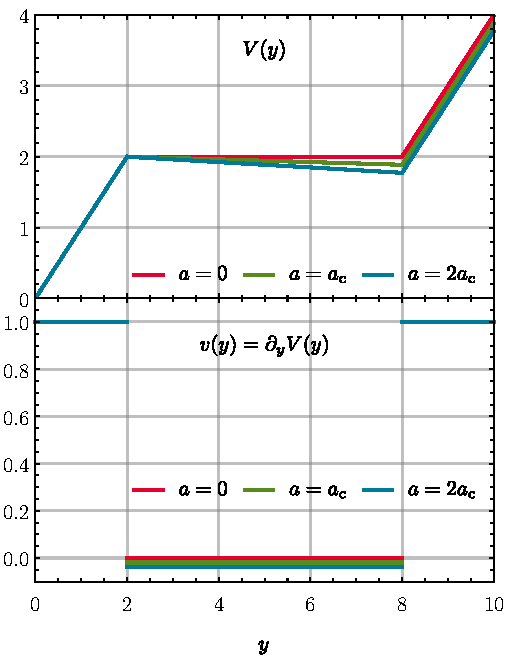
\includegraphics[width=\subcaptionFigureWidth+0.145cm]{0d/figures/Vofy.pdf}} % left figure
	{\vspace{-0.06cm}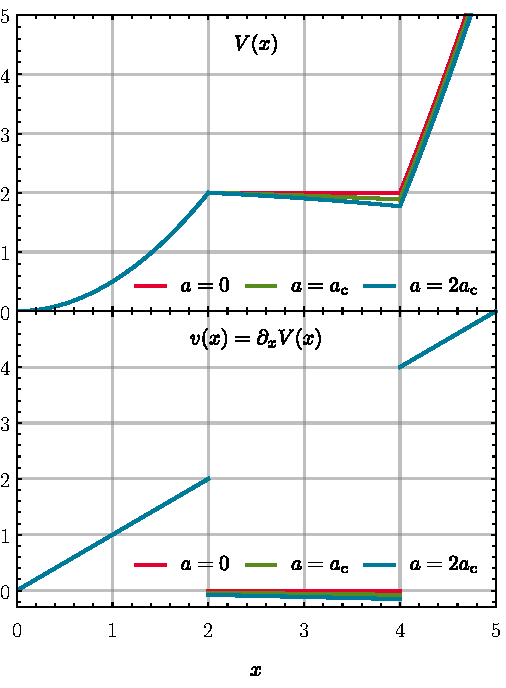
\includegraphics[width=\subcaptionFigureWidth-0.145cm]{0d/figures/Vofx.pdf}} % Right figure
	[fig:Vofy,fig:dVofy,fig:Vofx,fig:dVofx]
	{%
		The potential $V ( y )$ from \cref{eq:RP_Vofy} in the upper, left panel \subref{fig:Vofy} and its $y$-derivative $v ( y ) = \partial_y V ( y )$ from \cref{eq:RP_vofy} in the lower, left panel
		\subref{fig:dVofy} as well as the corresponding potential $V ( x )$ from \cref{eq:RP_Vofx} in the upper, right panel \subref{fig:Vofx} and its $x$-derivative $v ( x ) = \partial_x V ( x )$ from \cref{eq:RP_vofx} in the lower, right panel \subref{fig:dVofx} for selected values of the parameter $a$ \dash{} with ${a_\mathrm{c}\simeq 0.018951}$ from~\cref{eq:a_critical}.
		\fromFigs{1 and 3}{zerod3}
	}%
	{fig:Vofxy}
\FloatBarrier

\paragraph{An instructive toy model}\phantomsection\label{paragraph:RP}\mbox{}\\%
In this paragraph we present an explicit $O(N)$~model, respectively its $\frac{1}{N}$-rescaled self-interaction potential $V(y)$, which turns out to be a rather instructive toy model when studied at large and infinite $N$. We consider a family of piecewise linear potentials
	\begin{align}
		V ( y ) =
		\begin{cases}
			y							&	\text{for} \quad 0 \leq y \leq 2 \, ,\\
			- a \, y + 2 \, ( a + 1 )	&	\text{for} \quad 2 < y \leq 8 \, ,\\
			y - 6 \, ( a + 1 )			&	\text{for} \quad y>8 \, ,
		\end{cases}	\label{eq:RP_Vofy}
	\end{align}
with a parameter $a\geq0$. The first derivative of $V ( y )$ presents as a simple piecewise constant function in the $\tfrac{1}{N}$-rescaled invariant $y$
	\begin{align}
	v ( y ) = \partial_y V ( y ) =
	\begin{cases}
		1	&	\text{for} \quad 0 \leq y \leq 2 \, ,\\
		- a	&	\text{for} \quad 2 < y \leq 8 \, ,\\
		1	&	\text{for} \quad y>8 \, ,
	\end{cases}	\label{eq:RP_vofy}
\end{align}
which is very similar to the \ic{} (32) studied in \ccite{Grossi:2019urj}. The potential \eqref{eq:RP_Vofy} and its $y$-derivative \eqref{eq:RP_vofy} are plotted in \cref{fig:Vofy,fig:dVofy} for illustrative purposes.
In \cref{fig:Vofx,fig:dVofx}, we also plot the potential and its derivative as functions of the rescaled field $x$, where $\tfrac{1}{2} \, x^2 \equiv y\equiv \tfrac{1}{2N} \, \vec{\phi}^{\, 2}$, which might be more familiar after the preceding discussions of \cref{sec:0dON}.
We recognize such an initial value problem with piecewise constant \ics{} involving a set of contact discontinuities as a series of Riemann problem in the context of conservation equations and \cfd{}, \cf{} \cref{sec:conservationLaws}.
When considering \cref{eq:RP_vofy} as the \ic{} of a conservation equation in $y$, \cf{} \cref{paragraph:infiniteNflowsY}, we are faced with two Riemann problems (one at $y=2$ and one at $y=8$) at the \uv{} initial scale.

This model has several interesting properties:
\begin{enumerate}
	\item	The expectation values of \cref{eq:ON_expectation_value_largeN} can be evaluated in terms of known functions.
	In the limit ${N \rightarrow \infty}$ the \ipi{} correlation functions can be computed analytically for all $a\geq0$.
	We will discover within this subsection that there are two distinct parameter regimes, which are particularly interesting when studying this problem within the saddle-point and \frg{} frameworks.
	
	\item	For certain parameters $a$, which are smaller than some critical value $a_\mathrm{c}$, the \ipi{} correlation functions $\Gamma^{(n)}$ \dash{} the underlying expectation values \eqref{eq:ON_expectation_value_largeN} \dash{} can be computed by means of a saddle-point expansion.
	For $a \geq a_\mathrm{c}$ the saddle-point expansion is not applicable.
	This is discussed in detail in the following \cref{subsubsec:saddle_point}.
	
	\item	The model under consideration presents initially as two Riemann problems in the \frg{}  (fluid-dynamic) framework.
	The distinct parameter regimes, ${0 \leq a \leq a_\mathrm{c}}$ and $a > a_\mathrm{c}$, present with qualitatively different \frg{} flows.
	The interpretation involving Riemann problems, its numerical solution, and its consequences are discussed in detail in \cref{subsubsec:FRGlargeN}.
	At this point we also want to remind the reader of the methodological introduction of \cref{subsec:hydroAdvection,subsec:hydroEuler} which will be of great relevance for this subsection \dash{} the discussion of \frg{} flows at large and infinite $N$.
\end{enumerate}\bigskip

\fullWidthTwoColumnFigureTable%
	[!t] % Placement
	{0d/figures/fofy.pdf} % Figure
	{fig:sp_fofy} % Figure label
	{%
		Plot of ${f ( y ) = V ( y ) - \tfrac{1}{2} \ln ( y )}$ for the potential~\eqref{eq:RP_Vofy} for selected values of the parameter $a$ \dash{} with ${a_\mathrm{c}\simeq 0.018951}$ from~\cref{eq:a_critical}. The local minima of $f ( y )$ are located at $y_0 = \tfrac{1}{2}$ and $y_{0, 2} = 8$, where $y_0$ ($y_{0, 2}$) presents as the unique global minimum for $0 \leq a < a_\mathrm{c}$ ($a > a_\mathrm{c}$). At $a = a_\mathrm{c}$ both minima coincide and present both as global minima of $f ( y )$. The non-analyticity of $f ( y )$ in $y_{0, 2} = 8$ inherited from the piecewise definition of $V ( y )$ is clearly visible in the plot.
		\fromFig{2}{zerod3}%
	} % Figure caption
	{%
		\renewcommand{\arraystretch}{1.15}
		\small
		\begin{tabular}{l | c c c}
			\toprule
			$N$			&	$a = 0$		&	$a = a_\mathrm{c}$	&	$a = 2\, a_\mathrm{c}$\\
			\midrule
			$2$			&	$0.356907$	&	$0.327332$ 			&	$0.299162$\\
			$32$		&	$0.962306$	&	$0.475285$			&	$0.087158$\\
			$\infty$	&	 $1$		&	$1$					&	$0.0625$\\
			\bottomrule
		\end{tabular}
	} % Table content
	{tab:Gamma2N}% Table label
	{%
		Reference values for selected $N$ and $a$ of ${\Gamma^{(2)} = N ( \langle \vec{\phi}^{\, 2} \rangle )^{- 1}}$ computed with the expressions \eqref{eq:InNV_a0} and \eqref{eq:InNV} as well as their large $N$ asymptotics.
		The exact analytical results are in some cases rather lengthy and therefore we present in those cases only six decimal digits for readability.
		\fromTab{I}{zerod3}%
	} % Table caption
For now, we turn to the computation of the correlation functions of the model under consideration.
Solutions in terms of known functions for the necessary integrals \eqref{eq:In_largeN} for the potential \eqref{eq:RP_Vofy} are presented in \cref{app:RP_integrals}.
In the limit ${N \rightarrow \infty}$ the direct computations of \cref{app:RP_integrals} revealed two distinct regimes in parameter space separated by
\begin{align}
	a_\mathrm{c} = \tfrac{1}{4} - \tfrac{1}{3} \ln ( 2 ) \simeq 0.018951 \, .	\label{eq:a_critical}
\end{align}
For the infinite-$N$ limit of the expectation values \eqref{eq:ON_expectation_value} we find,
\begin{align}
	\lim_{N \rightarrow \infty} \tfrac{1}{N^n} \, \big\langle ( \vec{\phi}^{\, 2} )^n \big\rangle =
	\begin{cases}
		1 \, ,		&	\text{for} \quad 0 \leq a \leq a_\mathrm{c} \, ,\\
		16^n \, ,	&	\text{for} \quad a>a_\mathrm{c} \, ,
	\end{cases}
\end{align}
For the corresponding \ipi{} correlation functions this implies in the limit ${N \rightarrow \infty}$
\begin{align}
	\Gamma^{(2)} =	\label{eq:two-point_exact}
	\begin{cases}
	1 \, ,				&	\text{for} \quad 0 \leq a \leq a_\mathrm{c} \, ,
	\\
	\tfrac{1}{16} \, ,	&	\text{for} \quad a>a_\mathrm{c} \, ,
\end{cases}
\end{align}
as well as for all $a \geq 0$ 
\begin{align}
	\forall n \neq 2 \quad \Gamma^{(n)} = 0 \, .	\label{eq:n-point_exact}
\end{align}
Thus, in the limit ${N \rightarrow \infty}$ and in terms of \ipi{} vertices the current model under consideration presents as a massive non-interacting theory for all $a \geq 0$, \cf{} \cref{eq:free_Gamma}.
The situation for $0\leq a<a_\mathrm{c}$ and the corresponding ``mass'' as well as the origin of the critical value $a_\mathrm{c}$ can be understood intuitively in the context of the saddle-point expansion discussed in \cref{subsubsec:saddle_point}.
The situations for $a =a_\mathrm{c}$ and $a >a_\mathrm{c}$ are more involved and not accessible with a saddle-point expansion. 
However, a study in the \frg{}  framework is possible and rather instructive as we will demonstrate in \cref{subsubsec:FRGlargeN}.
In terms of correlation functions the theory undergoes a first-order phase transition at $a_\mathrm{c}$ when varying the external parameter $a$, \cf{} Sec.~III.C of \ccite{Grossi:2019urj} and references therein.

For finite $N$ higher-order \nptFunctions{} do not vanish and the theory is of ``interactive type'', but in the scope of this subsection we nevertheless mainly focus on $\Gamma^{(2)}$ \dash{} especially when it comes to numerical computations. In \cref{tab:Gamma2N} we summarize several (exact) reference values for $\Gamma^{(2)}$ for later use.

\FloatBarrier
\subsubsection{The saddle-point expansion at large \texorpdfstring{$N$}{N}}\label{subsubsec:saddle_point}
\begin{disclaimer}
	This subsubsection follows Sec. III of \ccite{Steil:2021cbu}.
\end{disclaimer}
In this subsubsection we will analyze the instructive toy model of \cref{paragraph:RP} within a saddle-point approximation for large $N$.
In \cref{app:saddle_point_app} we discuss the large-$N$ saddle-point expansion of integrals like \eqref{eq:In_largeN} concluding in the asymptotic series \eqref{eq:SPapp_series} for $\langle ( \vec{\phi}^{\, 2} )^n \rangle$.
To apply the series \eqref{eq:SPapp_series} to the interaction potential \eqref{eq:RP_Vofy} of the model under consideration, we first have to compute the global minimum $y_0$ of the exponents of the integrands in \cref{eq:ON_expectation_value_largeN},
\begin{align}
	f ( y ) = V ( y ) - \tfrac{1}{2} \ln ( y ) \, ,\label{eq:fofy}
\end{align}
and check for analyticity of $f ( y )$ and $g ( y ) = y^{n - 1}$ around $y_0$.
The function $f ( y )$ for the model under consideration is plotted in \cref{fig:sp_fofy} for different parameters $a$.

There is always a minimum on the first section (${0 \leq y \leq 2}$) of the piecewise linear potential
\begin{align}
	0 \overset{!}{=} \, & \partial_y f(y) \big|_{y = y_0} =	\, \bigg[ \partial_y V ( y ) - \frac{1}{2 y} \bigg]_{y = y_0} =\, 1 - \frac{1}{2 y_0} \, .
\end{align}
It follows that
\begin{align}
	&	y_0 = \tfrac{1}{2} \, ,	\qquad	V ( y_0 ) = \tfrac{1}{2} \, ,	\qquad	f ( y_0 ) = \tfrac{1}{2} \, \big[ 1 - \ln \big( \tfrac{1}{2} \big) \big] \, ,
\end{align}
and for the second and third derivatives, we find
\begin{align}
	&	\partial_y^2 V ( y ) \big|_{y = y_0} = 0 \, ,	&&	\partial_y^2 f ( y ) \big|_{y = y_0} = 2 \, ,\\[.2em]
	&	\partial_y^3 V ( y ) \big|_{y = y_0} = 0 \, ,	&&	\partial_y^3 f ( y ) \big|_{y = y_0} = - 8 \, .	
\end{align}
We note that $V ( y )$ and therefore also $f ( y )$ are smooth, thus $C^\infty$, and analytic around $y_0 = \tfrac{1}{2}$. Also $g ( y ) = y^{n - 1}$ is analytic and $C^\infty$ around $y_0 = \tfrac{1}{2}$. We can therefore use the asymptotic series \eqref{eq:SPapp_series} to compute the non-vanishing expectation values,
\begin{subequations}
\begin{align}
	\tfrac{1}{N} \, \langle \vec{\phi}^{\, 2}  \rangle = \, & 1 \, ,\\
	\tfrac{1}{N^2} \, \langle ( \vec{\phi}^{\, 2} )^2 \rangle = \, & 1 + \tfrac{2}{N} \, ,\\
	\tfrac{1}{N^3} \, \langle ( \vec{\phi}^{\, 2} )^3 \rangle = \, & 1 + \tfrac{6}{N} + \tfrac{8}{N^2} \, ,\\* % no page break here
	\vdots \mkern7.0mu  & \nonumber
\end{align}
\end{subequations}
and the corresponding \ipi{} correlation functions
\begin{align}
	&	\Gamma^{(2)} = 1 \, ,	&&	\forall n \neq 2 \quad \Gamma^{(n)} = 0 \, .
\end{align}
Both are exact results (without taking any limits) and we find that $\tfrac{1}{N^n} \, \langle ( \vec{\phi}^{\, 2} )^n \rangle = 1 + \order ( N^{- 1} )$, while the maximal correction to $1$ is always of $\order ( N^{- ( n - 1 )})$.
Considering the corresponding $\Gamma^{(2n)}$ we recover the \ipi{} correlation functions of a free massive theory, see \cref{eq:free_Gamma} with $m^2 = 1$, which \dash{} as an exact and $N$-independent result \dash{} also holds trivially in leading order in the limit ${N \rightarrow \infty}$.
This is a rather unsurprising result since the $\tfrac{1}{N}$-rescaled potential $V ( y )$ manifests as a linear potential with slope $1$ \dash{} corresponding to a non-interacting theory with $m^2 = 1$ \dash{} for ${0 \leq y \leq 2}$.\bigskip

The previous large-$N$ saddle-point approximation is however limited to potentials \eqref{eq:RP_Vofy} with $0 \leq a < a_\mathrm{c}$.
For $a\geq a_\mathrm{c}$ the function ${f ( y ) = V ( y ) - \tfrac{1}{2} \ln ( y )}$ develops a global minimum at $y_{0,2} = 8$, which becomes the unique global minimum for $a>a_\mathrm{c}$ while at $a=a_\mathrm{c}$ both $y_0$ and $y_{0,2}$ are global minima, see \cref{fig:sp_fofy}. 
For $a\geq a_\mathrm{c}$ the saddle-point expansion breaks down since at $a=a_\mathrm{c}$ the function $f(y)$ has no unique minimum and for $a>a_\mathrm{c}$ the function $f(y)$ is non-analytic in its global minimum (the ``expansion point'') $y_{0,2}=8$.
The value of $a_\mathrm{c}$ and the related qualitatively distinct scenarios were established in \cref{paragraph:RP}.
In the corresponding exact computations of \cref{app:RP_integrals} the threshold ${a_\mathrm{c}= \tfrac{1}{4} - \tfrac{1}{3} \ln ( 2 ) \simeq 0.018951}$ appears when considering the limit ${N \rightarrow \infty}$ of rather complicated symbolic expressions.
On the other hand, within the framework of the saddle-point expansion the value of $a_\mathrm{c}$ can be derived and understood in a very instructive way as the breakdown point of the saddle-point expansion,
\begin{subequations}\label{eq:saddle_minima}
	\begin{align}
		f \big( y_0 = \tfrac{1}{2} \big) \overset{!}{=} \, & f ( y_{0,2} = 8 )\\[.2em]
		\tfrac{1}{2} - \tfrac{1}{2} \ln \big( \tfrac{1}{2} \big) = \, & 8 - 6 \, ( a_\mathrm{c} + 1 ) - \tfrac{1}{2} \ln ( 8 ) \, ,
	\end{align}
\end{subequations}
which is solved again by
	\begin{align}
		a_\mathrm{c} = \, & \tfrac{1}{4} - \tfrac{1}{3} \ln ( 2 ) \simeq 0.018951 \, .
	\end{align}
	For $a<a_\mathrm{c}$ the model presents as a free massive theory in its saddle-point and the analytical results in the limit ${N \rightarrow \infty}$ of \cref{paragraph:RP} make perfect sense.
	
	In this subsection we are not interested in a quantitative review of the large-$N$ saddle-point expansion beyond the limit ${N \rightarrow \infty}$.
	For such a discussion in the context of zero-dimensional $O(N)$~models we refer the interested reader to the excellent and pedagogical \ccite{Keitel:2011pn}.
	
	At and beyond the critical value $a_\mathrm{c}$ \dash{} at and beyond the corresponding first-order phase transition \dash{} the saddle-point expansion is no longer applicable and alternative methods are required for the computation of correlation functions.
	Apart from the direct symbolic computations of \cref{paragraph:RP} the \frg{} has proven to be a potent tool for computations in zero dimensions at finite $N$, \cf{} \cref{subsec:0dONresults,subsec:0dO1Entropy},  and as we will demonstrate in \cref{subsubsec:FRGlargeN} it loses none of its potency in the infinite-$N$ limit when employing proper numerical schemes, like the \kt{} and \knpScheme{}.

\subsubsection{FRG flow equations at large and infinite \texorpdfstring{$N$}{N}}\label{subsubsec:FRGlargeN}
\begin{disclaimer}
	This subsubsection follows Sec. IV and App. E of \ccite{Steil:2021cbu}.
\end{disclaimer}
We proceed with our \frg{} studies at large and infinite $N$ using our established \cfd{} methods and concepts.

\paragraph{The \texorpdfstring{$\tfrac{1}{N}$}{1/N}-rescaled FRG flow equation}\phantomsection\label{paragraph:FRGlargeN1overN}\mbox{}\\%
To facilitate the studies at large $N$ and in the limit $N\rightarrow\infty$, we have to rescale the flow \cref{eq:conservation_law_u_phi,eq:conservation_law_u_rho} according to \cref{paragraph:zerodOinfRescaling}.

To this end, we make use of the rescalings \eqref{eq:rescalings} of extensive quantities,
	\begin{align}
		&	\sigma \mapsto x = \tfrac{1}{\sqrt{N}} \, \sigma \, ,	&&	U ( t, \sigma ) \mapsto V ( t, x ) = \tfrac{1}{N} \,  U ( t, \sigma ) \, .
	\end{align}
and additionally introduce $v ( t, x ) \equiv \partial_x V ( t, x )$,
	\begin{align}
		u ( t, \sigma ) \mapsto v ( t, x ) = \tfrac{1}{\sqrt{N}} \, u ( t, \sigma ) \, .
	\end{align}
On the level of the \frg{} flow equation, this results in a slight modification of the prefactors of the fluxes \eqref{eq:advection_flux_pion_propagator} and \eqref{eq:diffusion_flux_sigma_propagator}.
The rescaled flow equation in $x$ follows as	
	\begin{align}
		\partial_t v ( t, x ) &=\, \dod{}{x}\! \bigg[ \frac{N - 1}{N} \, \frac{\tfrac{1}{2} \, \partial_t r ( t )}{r ( t ) + \frac{1}{x} \, v ( t, x )} + \frac{1}{N} \, \frac{\tfrac{1}{2} \, \partial_t r ( t )}{r ( t ) + \partial_x v ( t, x )} \bigg] \, ,\label{eq:frg_flow_x}
	\end{align}
which makes it easily possible to take the infinite-$N$ limit and to compare \frg{} flows for infinite and finite values of $N$. 
Already at this point we find that increasing $N$ makes the problem more and more advection driven.
In the limit $N \rightarrow \infty$ the diffusion flux vanishes completely and we are left over with the infinite-$N$ flow equation,
\begin{align}
	\partial_t v ( t, x ) = \, & \dod{}{x}\! \bigg[ \frac{\tfrac{1}{2} \, \partial_t r ( t )}{r ( t ) + \frac{1}{x} \, v ( t, x )}\bigg] \, . \label{eq:frg_flow_Ninf_x}
\end{align}
This \pde{} presents as an advective hyperbolic conservation law, \cf{} \cref{subsec:hydroAdvection}, and is very similar to its higher-dimensional counterpart~\cite{Tetradis:1995br,Litim:1995ex,Grossi:2019urj}.

Of course, we can also formulate the \frg{} flow equation \eqref{eq:frg_flow_x} as a fluid-dynamic problem in the $\tfrac{1}{N}$-rescaled invariant $y = \tfrac{1}{2} \, x^2$,
	\begin{align}
		\partial_t v ( t, y ) & = \, \dod{}{y}\! \bigg[ \frac{N - 1}{N} \, \frac{\tfrac{1}{2} \, \partial_t r ( t )}{r ( t ) + v ( t, y )} + \frac{1}{N} \, \frac{\tfrac{1}{2} \, \partial_t r ( t )}{r ( t ) + v(t,y) +2 y \, \partial_y v ( t, y )} \bigg] \, ,	\label{eq:frg_flow_y}
	\end{align}
as is done in \ccite{Grossi:2019urj,Grossi:2021ksl}.
Overall the structure of the equation keeps its conservative form in terms of an advection-diffusion equation\footnote{This generalizes in $x$ and $y$ to arbitrary dimensions and also to the fixed-point form of the \frg{} flow equation~\cite{Koenigstein:2021syz,Koenigstein:2021rxj,Stoll:2021ori}. 
Regarding fixed points in the infinite-$N$ limit for the $O(N)$~model in the \frg{} context we refer the interested reader to \ccite{Litim:2016hlb,Litim:2018pxe} for a detailed discussion of the situation in $d=3$ dimensions.}.

The main difference is that the advective contribution lost its unpleasant position-dependence, which is now found in the second (formerly purely diffusive) contribution. 
The diffusive term has changed drastically and can no longer be exclusively interpreted as a non-linear diffusion flux, \cf{} the related discussion in \cref{subsec:hydroDiffusion}. 

In \cref{subsubsec:conservative_form,subsec:boundary_conditions_finite_volume} we argued at length, that, due to several reasons, we currently believe that a formulation in $x$ instead of $y$ is favorable as soon as we allow for diffusive contributions to the \frg{} flow \dash{} hence at finite $N$. 
In \cref{subsec:boundary_conditions_finite_volume} we discuss the difficulties arising when attempting to formulate the inevitable spatial boundary condition at $y = 0$, when using the (rescaled) invariant $y$. 
An oversimplified argument is that there is no physical meaning of negative values of $y$, which makes a correct formulation of a boundary condition, that correctly captures possible influx due to diffusion, extremely challenging \dash{} if not impossible. 
In a formulation in $x$, this is not a problem at all, since negative $x$ formally exist and antisymmetric boundary conditions can be used for $u ( t, x )$ at $x = 0$. 
Additionally, it is understandable that a sober split of advection and diffusion fluxes is no longer possible in $y$, by simply executing the total $y$-derivative on the \rhs{} of \cref{eq:frg_flow_y} for the last term.
Hence, as long as $N$ is finite, one has to live with the challenging $x$-dependence in the advection flux of the \pde{} \eqref{eq:frg_flow_x}, which can however be handled by suitable discretizations, as demonstrated at length in \cref{subsec:FRG-formulationONmodel,subsec:0dONresults}.

However, in the infinite-$N$ limit the second term of the \pde{} \eqref{eq:frg_flow_y} vanishes and the problem again reduces to a hyperbolic non-linear advection equation \dash{} without any explicit position-dependencies,
	\begin{align}
		\partial_t v ( t, y )  &= \, \dod{}{y} \!\bigg[ \frac{\tfrac{1}{2} \, \partial_t r ( t )}{r ( t ) + v ( t, y )} \bigg]\equiv - \dod{}{y} G [ t, v ]  = - (\partial_v G [ t, v ]) \partial_y v(t,y)\, . \label{eq:frg_flow_Ninf_y}
	\end{align}
Because the newly defined advection flux $\partial_v G [ t, v ]$ has manifestly negative sign \dash{} \cf{} \cref{eq:frg_flow_Ninf_yExp}, there can not be any influx at $y = 0$ into the spatial domain $y \in [ 0, \infty )$ of the problem resolving the conceptual issues with the $y = 0$ boundary and allowing practical computations in the rescaled invariant $y$.
Note that the computations of \ccite{Grossi:2019urj,Grossi:2021ksl,Ihssen:2023xlp} use this zero influx argument for their computations with discontinuous Galerkin methods in the invariant $\varrho$/$y$.

\paragraph{The \knp{} scheme}\phantomsection\label{paragraph:knpLargeN} can be used to solve the flow equation in the invariant $y$ in the infinite $N$-limit.
For the problematic left boundary we consider the primitive form in \cref{eq:frg_flow_Ninf_y} using
\begin{align}
	\frac{\partial G}{\partial v}= -\frac{1}{2} \frac{\Lambda\eu^{-t}}{(\Lambda\eu^{-t} + v)^2}\, . \label{eq:frg_flow_Ninf_yExp}
\end{align}
For all $y\in\Reals{}^+$ and $t\in\Reals{}^+$ $\partial_v G [ t, v ] < 0$, holds for all well-defined initial conditions, which realize $r ( t ) + v ( t, y ) > 0$ at $t=0$. 

\Cref{eq:frg_flow_Ninf_yExp} is manifest negative and finite for all $y\in\Reals{}^+$ and $t\in\Reals{}^+$ for all valid initial conditions/\uv{} initial scales realizing $\Lambda \, \eu^{-t} + v>0$ in the \uv{}.
The latter inequality is guaranteed dynamically at $t > 0$ by the flow equation as long as it is realized in the \uv{} at the initial scale $t = 0$, \cf{} \cref{eq:LambdaMin} and the related discussion of \rgcy{} \cref{paragraph:ONRGconsistency}.
This however implies in \cref{eq:FVapjp12} a vanishing right-sided local speed $a_{j + \ttfrac{1}{2}}^+=0$.
Physically this means that the fluid is only propagated to the left which simplifies the expression \eqref{eq:definition_h_knp_scheme} for the numerical flux of the \knp{} scheme immensely
\begin{align}
	H_{j + \frac{1}{2}}^{\mathrm{KNP}} \big|_{a_{j + \frac{1}{2}}^+ = 0} = G [ t, v_{j + \frac{1}{2}}^+ ]
\end{align}
resulting in the numerical upwind advection flux for the \knp{} scheme
\begin{align}
	\partial_t \bar{v}_j = \tfrac{1}{\Delta y} \, \big( G [ t, v_{j - \frac{1}{2}}^+] - G [ t, v_{j + \frac{1}{2}}^+ ] \big) \, .	\label{eq:FV_KNP_monotone}
\end{align}
It is this reduction to an upwind scheme in regions with directed local speeds equivalent to monotonic advection fluxes with either $a_{j + \ttfrac{1}{2}}^+ = 0$ or $a_{j + \ttfrac{1}{2}}^- = 0$, which has led the authors of \ccite{KTO2-1} to call their scheme a central-upwind scheme.
Note that \cref{eq:FV_KNP_monotone} does no longer include the left-sided local speed $a_{j + \ttfrac{1}{2}}^-$ and only contains advection terms evaluated at $v_{j\pm\ttfrac{1}{2}}^+$ involving the reconstructions from the cells to the right, \cf{} \cref{eq:FVupjp12} and \eqref{eq:FVuxjn}.
As a result the numerical flux of \cref{eq:FV_KNP_monotone} is based on a right-leaning four-point stencil ${\{\bar{v}_{j-1},\bar{v}_j,\bar{v}_{j+1},\bar{v}_{j+2}\}}$, where $\bar{v}_{j-1}$ is required together with $\bar{v}_{j}$ and $\bar{v}_{j+1}$ to compute $( \partial_y v )_j$.
For the numerical flux of the first volume cell $j=0$ which we choose to span over $y_{-\ttfrac{1}{2}}=0$ to $y_{\ttfrac{1}{2}}=\Delta y$ we require ${\{\bar{v}_{-1},\bar{v}_0,\bar{v}_{1},\bar{v}_{2}\}}$, where only $\bar{v}_{-1}$ is a ghost cell.
Since it only appears in the flux limiting procedure, see \eqref{eq:FVuxjn}, it is arguably not a ghost point related to physical boundary conditions but rather a computational one necessary to ensure formal second-order accuracy of the \muscl{} reconstruction while preventing spurious oscillations around discontinuities \dash{} \tvd{} time steps. 

Two naive strategies for a practical choice of $\bar{v}_{-1}$ come to mind.
The first one would be switching from a central reconstruction to a right-sided reconstruction.
Constructing a right-sided \tvd{} reconstruction or searching for one in literature seemed unappealing for our limited discussion of this subsection.
The second option is much simpler and related to the fact, that the \knp{} scheme with the position-independent advection flux $G$ of \cref{eq:frg_flow_Ninf_y} has a meaningful first-order reduction. 
Switching from a piecewise linear to a piecewise constant reconstruction in \cref{eq:FVumpjp12}:
\begin{subequations}\label{eq:FV_up12mp1st}
\begin{align}
	v_{j + \frac{1}{2}}^{-} = \, & \bar{v}_j + \order ( \Delta y ) \, ,\label{eq:FV_up12m1st}\\[.1em]
	v_{j + \frac{1}{2}}^{+} = \, & \bar{v}_{j+1} + \order ( \Delta y ) \, ,\label{eq:FV_up12p1st}
\end{align}
\end{subequations}
results in a first-order accurate (in $\Delta y$) semi-discrete upwind scheme~\cite{KTO2-1,10.2307/2157317,10.2307/2030019}
\begin{align}
	\partial_t \bar{v}_j = \tfrac{1}{\Delta y} \, \big( G[t,\bar{v}_{j}] - G[t,\bar{v}_{j + 1}] \big) \, , \label{eq:FV_KNP_monotone1st}
\end{align}
valid for monotone advection fluxes with $\partial_u G<0$.
The first-order accurate \knp{} scheme is in this context equivalent to the so-called Godunov upwind scheme~\cite{10.2307/2157317,10.2307/2030019}.
Application of such first-order upwind-schemes within the \frg{} framework are discussed and presented in \ccite{Wink:2020tnu,WinkHirschegg}.
To avoid the ghost cell $\bar{v}_{-1}$ altogether we always use the first-order accurate \knp{} scheme \eqref{eq:FV_KNP_monotone1st} for the explicit results discussed in the following.
Selected results with the second-order accurate \knp{} scheme can be found in \LargeNnumApp{}.
	
We conclude this paragraph with a brief remark on the \kt{} scheme.
Using the conservative, equal sided estimate ${a_{j + \ttfrac{1}{2}}^+ = -a_{j + \ttfrac{1}{2}}^-=a_{j + \ttfrac{1}{2}}}$ for the right- and left-sided local speeds $a_{j + \ttfrac{1}{2}}^\pm$, the numerical advection flux \eqref{eq:definition_h_knp_scheme} of the \knp{} scheme reduces to the advection flux the \kt{} scheme
\begin{align}
	H_{j + \frac{1}{2}}^{\mathrm{KT}} \equiv \, & \frac{G \big[ t, v_{j + \frac{1}{2}}^+ \big] + G \big[ t, v_{j + \frac{1}{2}}^- \big]}{2} - a_{j + \frac{1}{2}} \, \frac{v_{j + \frac{1}{2}}^{+} - v_{j + \frac{1}{2}}^{-}}{2} \, ,	\label{eq:FV_KT_H}
\end{align}
with
\begin{align}
	 a_{j + \frac{1}{2}} \equiv \max \bigg\{ \bigg| \frac{\partial G}{\partial v} \Big[ t, v_{j + \frac{1}{2}}^{+} \Big] \bigg| , \bigg| \frac{\partial G}{\partial v} \Big[ t,v_{j + \frac{1}{2}}^{-} \Big] \bigg| \bigg\} \, . \label{eq:FV_KT_ajp12}
\end{align}
In the first volume cell $\bar{v}_{-1}$ appears outside of the flux limiting procedure and is also present in the first-order accurate reduction of the \kt{} scheme \eqref{eq:FV_KT_H} using Eqs.~\eqref{eq:FV_up12m1st} and \eqref{eq:FV_up12p1st} since the latter is based on a central scheme based on the stencil ${\{\bar{v}_{j-1},\bar{v}_j,\bar{v}_{j+1}\}}$.
Lacking the more refined estimates for the right- and left-sided local speeds $a_{j + \ttfrac{1}{2}}^\pm$ of the \knp{} scheme it is not obvious how to deal with the ghost cell at $\bar{v}_{-1}$. This is, why we chose the \knp{} scheme for our numerical computations in $y$. 
The advection flux of the \knp{} scheme is also suited for the position depended advection flux $F$ of the flow equation \eqref{eq:frg_flow_Ninf_x} in $x$.
We have performed some heuristic tests with the \knp{} scheme and the flow equation \eqref{eq:frg_flow_Ninf_x} in $x$ and we come to the preliminary conclusion that it is in terms of accuracy and performance on par with the \kt{} scheme in this scenario.
Nevertheless, further detailed tests might be of interest for upcoming challenges in the context of \frg{} problems in $d > 0$ with more sophisticated truncations.

\paragraph{The \uv{} initial condition} for the flows in $v(y)$ and $v(x)$ are visualized in \cref{fig:dVofy,fig:dVofx}.
For the \frg{} flow equations \eqref{eq:frg_flow_x} and \eqref{eq:frg_flow_Ninf_x} the initial conditions \eqref{eq:RP_Vofy} and \eqref{eq:RP_vofy} have to be transformed to the variable $x$. For the one parameter family of \uv{} potentials, this reads
	\begin{align}
		V ( x ) =
		\begin{cases}
			\tfrac{1}{2} \, x^2							&	\text{for} \quad |x| \leq 2 \, ,\\[.1em]
			- a \, \tfrac{1}{2} \, x^2 + 2 \, ( a + 1 )	&	\text{for} \quad 2 < |x| \leq 4 \, ,\\[.1em]
			\tfrac{1}{2} \, x^2 - 6 \, ( a + 1 )		&	\text{for} \quad |x|>4 \, .
		\end{cases}\label{eq:RP_Vofx}
	\end{align}
Hence, our \uv{} potential is actually a piecewise quadratic function of $x = \tfrac{1}{\sqrt{N}} \, \sigma$, while its $x$-derivative is given by the piecewise linear function
	\begin{align}
		v ( x ) = \partial_x V ( x ) =
		\begin{cases}
			x		&	\text{for} \quad |x| \leq 2 \, ,\\[.1em]
			- a \, x	&	\text{for} \quad 2 < |x| \leq 4 \, ,\\[.1em]
			x		&	\text{for} \quad |x|>4 \, .
		\end{cases} \label{eq:RP_vofx}
	\end{align}

\FloatBarrier
\subsubsection{FRG flows at infinite \texorpdfstring{$N$}{N} -- shocks and rarefaction waves in advective flows}\label{subsubsec:FRGlargeNinf}
\begin{disclaimer}
	This subsubsection follows Sec. IV.E and App. E of \ccite{Steil:2021cbu}.
\end{disclaimer}
Next, we turn to the results for the \frg{} flows for \cref{eq:RP_vofx} in the limit $N \rightarrow \infty$.
Before presenting the numerical results, which are obtained by a numerical solution of the \pde{} \eqref{eq:frg_flow_Ninf_x} with the \kt{}/\knp{} scheme~\cite{KTO2-0,KTO2-1}, we use the method of characteristics to discuss analytic results for solutions of the purely hyperbolic conservation law \eqref{eq:frg_flow_Ninf_x}.
This helps to better understand the underlying processes in the fluid-dynamical framework and the results of our numeric calculations.

In the \frg{} framework the method of characteristics was used by N. Tetradis and D.~Litim in \ccite{Tetradis:1995br,Litim:1995ex} to obtain analytical solutions to \frg{} flow equations of the $O(N)$~model in dimensions $d > 0$ in the infinite-$N$ limit. 
K.-I. Aoki, S.-I. Kumamoto, D. Sato, and M. Yamada also used the method of characteristics and the Rankine-Hugoniot condition in their studies~\cite{Aoki:2014,Aoki:2017rjl} of weak solutions and dynamical symmetry breaking. 
Unfortunately (or luckily for my collaborators and me and our works~\cite{Grossi:2019urj,Grossi:2021ksl,Koenigstein:2021syz,Koenigstein:2021rxj,Steil:partIV,Stoll:2021ori}), their otherwise remarkable work lacks the fluid-dynamical interpretation and with it an instructive way to understand characteristic curves in this context.
The latter was put forward in the context of the \frg{} for the first time in \ccite{Grossi:2019urj}.\bigskip
\subcaptionFigureWidthFigure%
	[!t]%
	{0d/figures/characteristics.pdf}% Graphics
	[]% Sublabels
	{%
{}%
		Selected characteristic curves $(t,x(t))$, see \cref{eq:MoC_xoftau}, for $a=0$ and $\Lambda=10^{10}$ in {blue}, {green} and {yellow}, shock position $\xi_\mathrm{s} ( t )$, see \cref{eq:xioft}, as solid black line, and the tips of the rarefaction fan $\xi_\mathrm{r}^\mp ( t )$, see \cref{eq:rarefaction_minus} and \eqref{eq:rarefaction_plus} originating at $( t = 0, \xi_\mathrm{r}^\mp ( 0 ) = 4 )$ as dashed black lines.
		The changing color on the characteristic curves indicates the change of $v(t,x(t))$ along them, see \cref{eq:MoC_vxoftau}, where {blue} corresponds to $v ( t, x ( t ) ) = 0$ and {yellow} corresponds to $v ( t, x ( t ) ) = 4.5$.
		The shock wave and the rarefaction fan collide at $( t, x ) \approx ( 25.718, 1.115 )$ (the time is marked with the {red-dashed} line) rendering the expressions $\xi_\mathrm{r}^\pm ( t )$ and $\xi_\mathrm{s} ( t )$ as well as the characteristics that intersect with the shock and rarefaction wave invalid for later times.
		\fromFig{4}{zerod3}
	}%Caption
	{fig:frg_largeNChar}%Label

\paragraph{Characteristic curves}\phantomsection\label{paragraph:largeNchars}\mbox{}\\%
The characteristic curves of the fluid are visualized in \cref{fig:frg_largeNChar}.
These are defined as those (parametric) curves $( t, x ( t ) )$ in the domain $[ 0, \infty ) \times ( - \infty, + \infty )$ of the problem, where the ratio $\frac{v ( t, x ( t ))}{x ( t )}$ stays constant\footnote{If formulated in terms of the $\frac{1}{N}$-rescaled invariant $y$, these are the (parametric) curves $( t, y ( t ) )$ on $[ 0, \infty ) \times [ 0, \infty )$, where $v ( t, y ( t ))$ is constant, see, \eg{}, \ccite{Grossi:2019urj}. Both formulations can be transformed into each other by simple coordinate transformations, see App.~\ref{app:method_of_characteristics}.}.
In \cref{app:method_of_characteristics} we derive these implicit analytic solutions for the \pde{} \eqref{eq:frg_flow_Ninf_x} with initial condition \eqref{eq:RP_vofx} in great detail and the explicit solutions for $x ( t )$ and $v ( t, x ( t ))$ are given by \cref{eq:MoC_xoftau} and \eqref{eq:MoC_vxoftau}. 
If needed, $x ( t )$ and $v ( t, x ( t ))$ can be used to reconstruct the full solution of the \pde{}, $v ( t, x )$, for $t \in [ 0, \infty )$ and $x \in ( - \infty, + \infty )$, which usually needs to be done numerically since the involved expressions can usually not be inverted analytically. 
Though, this method only works as long as the solution $v ( t, x )$ is not multi-valued, which means that it is valid until any characteristics intersect at some point $x$ in position space  (here field space).
Once the analytical solution becomes multi-valued, the physical solution exists only in a weak sense, see, \eg{}, \ccite{Ames:1992,LeVeque:1992,LeVeque:2002,Hesthaven2007,RezzollaZanotti:2013} or \cref{sec:conservationLaws} for details. Intersecting characteristics correspond to the formation of a shock wave, since several fluid elements are approaching the same point in the spatial domain at different velocities~\cite{Ames:1992,LeVeque:1992,LeVeque:2002,Hesthaven2007,RezzollaZanotti:2013}. 
The movement of this shock wave, its (parametric) curve $( t, \xi_\mathrm{s} ( t ) )$, is described by the Rankine-Hugoniot shock condition~\cite{Rankine:1870,Hugoniot:1887}.
A derivation is presented in \cref{app:rankine-hugoniot_condition_and_shock_position}.
On the other hand, there might also be positions in field space that ``separate'' the characteristic curves into distinct regimes and that are the origin of infinitely many characteristic curves. 
These are so-called \textit{rarefaction waves}, which each cause a \textit{rarefaction fan} of infinitely many characteristic curves. As their name suggests, they are associated to points $x$ (in field space), where fluid elements are moving apart from each other and cause a rarefaction of the fluid (in physical fluids corresponding to a reduction of density as a direct opposite of a compression wave), \cf{} \cref{subsec:hydroEuler}.
A rarefaction fan can be described by the spatially closest characteristic curves  $( t, \xi^\mp_\mathrm{r} ( t ) )$ that are moving to the left ($-$) and right ($+$) apart from each other.

Now we are equipped with the vocabulary to efficiently interpret and analyze \cref{fig:frg_largeNChar}.
\WlogA{} we choose the initial condition \eqref{eq:RP_vofx} with $a = 0$ \dash{} the plots and the discussion for different choices of $a$ are qualitatively very similar.
Furthermore, we only restrict our plot of the characteristics and parts of the discussion to positive $x$. For negative $x$ the dynamics is perfectly mirrored about the $t$ axis in \cref{fig:frg_largeNChar}.

The initial condition $v ( t = 0, x ) = v ( x )$ corresponds to the initial values of $v ( t, x ( t ) )$ on the characteristic curves at $t = 0$ along the $x$-axis. The color-coding indicates the value of $v ( t, x ( t ) )$ according to \cref{eq:MoC_vxoftau} along the curves $( t, x ( t ) )$, where {blue} corresponds to $v ( t, x ( t ) ) = 0$ and {yellow} corresponds to $v ( t, x ( t ) ) = 4.5$. 

Firstly and in general, we observe that all characteristic curves only move towards smaller $| x |$, while $v ( t, x ( t ) )$ only decreases (increases) along each characteristic curve at positive (negative) $x$. This implies that the fluid $v ( t, x)$ only moves towards $x = 0$. This can already be seen from the manifestly (positive) negative sign of the local fluid velocity $\partial_v F [ t, x, v ]$ for (negative) positive $x$, \cf{} \cref{eq:advection_flux_pion_propagator} and \cref{eq:frg_flow_Ninf_y}. Hence, we find that right-moving waves of the fluid from negative $x$ and left-moving waves of the fluid from positive $x$ annihilate in $x = 0$, which is also manifestly encoded in the antisymmetry $v ( t, x ) = - v ( t, - x)$.

Secondly we observe that the fluid elements, which start off in the interval $2 < | x | < 4$, move faster towards $x = 0$ than the fluid elements, that start at $| x | < 2$. As soon as the former try to overtake the latter, the solution gets multi-valued and a shock forms. Actually, this happens already at $t = 0$, but we can also see how more and more characteristics ``join'' and ``accelerate'' the shock wave. The movement of the shock wave,$( t, \xi_\mathrm{s} ( t ))$ is described analytically by \cref{eq:xioft} and depicted as a black solid line in \cref{fig:frg_largeNChar}.

Thirdly, there is another important phenomenon going on around $| x | = 4$. We find that fluid elements at $| x | < 4$ are traveling fast towards $x = 0$, while the characteristic curves that start at $| x | > 4$ move slower towards $x = 0$ and that only for a very short period of (RG) time, before the characteristic curve closest to $|x| = 4$ freezes at ${| x | \simeq \sqrt{15} \simeq 3.873}$. This effectively causes a rarefaction wave in $v ( t, x )$, which is described analytically by
	\begin{align}
		\xi_\mathrm{r}^- ( t ) = \, & \pm \sqrt{16 - \frac{1}{\Lambda \, \eu^{- t} - a} + \frac{1}{\Lambda - a} } \, ,	\label{eq:rarefaction_minus}
		\\
		v_\mathrm{r}^- ( t ) = \, & - a \, \xi_\mathrm{r}^- ( t ) \, ,\\[.2em]
		\xi_\mathrm{r}^+ ( t ) = \, & \pm \sqrt{16 - \frac{1}{\Lambda \, \eu^{- t} + 1} + \frac{1}{\Lambda + 1} } \, ,	\label{eq:rarefaction_plus}
		\\
		v_\mathrm{r}^+ ( t ) = \, & \xi_\mathrm{r}^+ ( t ) \, ,	
	\end{align}
where $v_\mathrm{r}^\mp ( t )$ are the values of of the fluid at the edges of the rarefaction fan. The rarefaction fan is marked in \cref{fig:frg_largeNChar} by black-dashed lines that are analytically described by \cref{eq:rarefaction_minus} and \eqref{eq:rarefaction_plus}. The rarefaction wave also forms already at $t = 0$.\\

Interestingly, there is a (RG) time and field space position $( t, x ) \simeq ( 25.718, 1.115 )$, where the rarefaction fan catches up the shock wave (indicated by the {red-dashed} horizontal line). Up to this point, our analytical solutions for the shock $\xi_\mathrm{s} ( t )$ and the left tip of the rarefaction wave $\xi_\mathrm{r}^- ( t )$ are valid and we could in principle even integrate backwards in (RG) time and reconstruct the \uv{} potential. However, when the shock and the rarefaction wave meet and interact, some highly non-linear dynamics is going on and we can no longer trust our analytical solutions. At later (RG) times, we have to rely on adequate numerical solutions.

Interestingly, it is exactly this complicated non-analytic dynamics, which makes the \frg{} flow manifestly irreversible and produces some abstract form of entropy, see \cref{paragraph:infiniteNflowsEntropy} and especially \cref{fig:frg_largeN_TVD} as well as \ccite{Koenigstein:2021syz,Koenigstein:2021rxj}, because information about the \uv{} initial potential is unavoidably lost. Actually, this is the dynamics that fundamentally encodes the irreversibility of \rg{} transformations on the level of the PDE, \cf{}\ also \ccite{Wilson:1979qg,Zumbach:1994vg,Zamolodchikov:1986gt} for similar discussions.

However, most remarkably in the context of the infinite-$N$ limit: We find numerically that it is the complicated interplay between the shock and rarefaction waves (at positive and negative $x$), which either causes the shock waves to freeze at some non-zero $|x|$ or to crash into each other and annihilate in $x = 0$, depending on the choice of $a$ \dash{} smaller, equal, or greater than $a_\mathrm{c}$. This means that the (non\nobreakdash-)applicability of the large-$N$ saddle-point expansion of \cref{subsubsec:saddle_point}, which was caused by a (non\nobreakdash-)analytic ``expansion point'' \dash{} the underlying first-order phase transition, translates into the freezing or the annihilation of shock waves in field space in \frg{} flow equations. For further details on the relation between first-order phase transitions and the interaction/freezing of shock and rarefaction waves we refer the interested reader to Sec.~III.C of \nbccite{Grossi:2019urj}. However, to proceed with this discussion and to understand this interrelation, we have to leave the sure ground of analytical solutions and turn to high precision numerical computations of this challenging dynamics.

\paragraph{Numerical results at infinite \texorpdfstring{$N$}{N} in \texorpdfstring{$x$}{x}}\phantomsection\label{paragraph:infiniteNflows}\mbox{}\\%
\subcaptionFigureVariableWidth%
	[!t]% placement
	[-0.262cm]% widthShift
	{% figA
		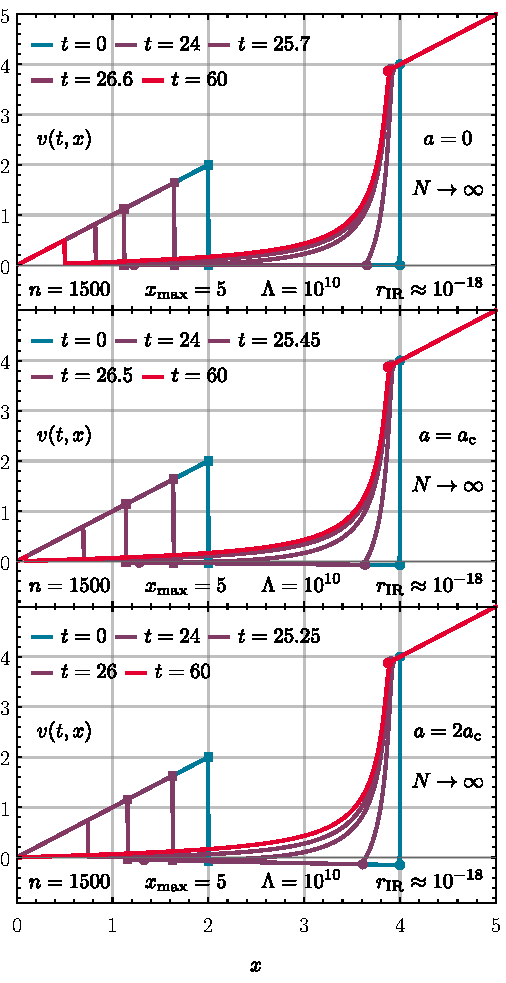
\includegraphics[width=\subcaptionFigureWidth-0.262cm]{0d/figures/largeN_flows.pdf}% figure (a)
		\captionsetup{font=footnotesize,width=\subcaptionFigureWidth-0.262cm}%
		\caption{\frg{} flow of the derivative of the rescaled effective potential $v ( t, x )$}% caption (a)
		\label{fig:frg_largeN}% label (a)
	}
	{\hspace{\subcaptionFigureSpacing}}% spacing
	{% figB
		\raisebox{-0.102cm}{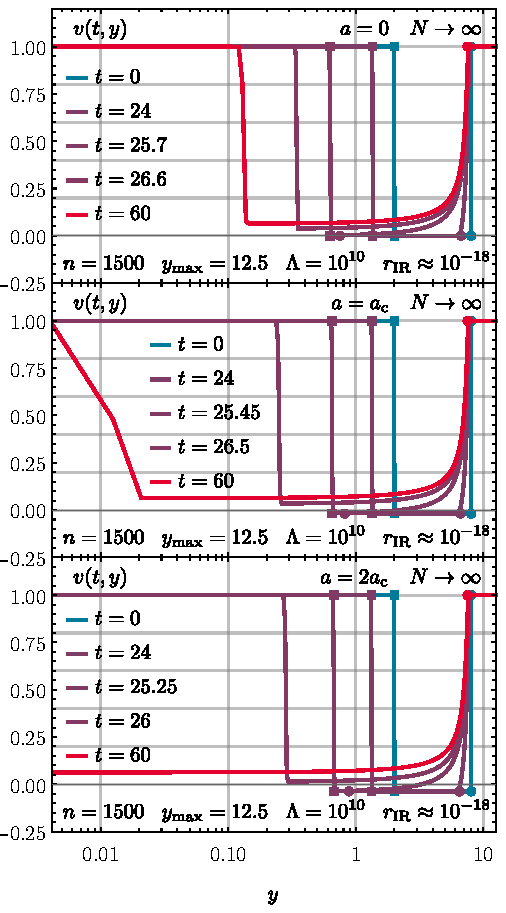
\includegraphics[width=\subcaptionFigureWidth+0.262cm]{0d/figures/largeN_KNPO1flows.pdf}}% figure (b)
		\captionsetup{font=footnotesize,width=\subcaptionFigureWidth+0.262cm}%
		\caption{%
			\frg{} flow of the derivative of the rescaled effective potential $v ( t, y )$.
			We choose a logarithmic scale for the $y$-axis for better visibility around $y = 0$ which is particularly useful for the visualization of the freezing shocks in the \ir{} for $a = 0$ and $a = a_\mathrm{c}$.%
		}% caption (b)
		\label{fig:frg_largeN_KNPO1_flows}% label (b)
	}
	{%
		\frg{} flows for the zero-dimensional $O(N)$ model in $x$ on the left \subref{fig:frg_largeN} and in the $\tfrac{1}{N}$-rescaled invariant $y \equiv \tfrac{1}{2} \, x^2$ on the right \subref{fig:frg_largeN_KNPO1_flows} in the limit $N \rightarrow \infty$ for the \ic{}~\eqref{eq:RP_vofx} with ${a = 0}$, ${a = a_\mathrm{c}}$, and ${a = 2 a_\mathrm{c}}$ in the upper, middle, and lower panel respectively.
		{Blue} curves represent the \uv{} initial conditions at $t=0$, {red} curves correspond to the \ir{} potentials at $t = 60$ and the {violet} curves are at intermediate, selected \rgtimes{} $t$ chosen around the respective collision of the shock $\xi_\mathrm{s} ( t ) $ with the left tip of the rarefaction fan $\xi_\mathrm{r}^{-}(t)$.
		The squares mark the shock $( \xi_\mathrm{s} ( t ), v ( t, \xi_\mathrm{s} ( t )^\pm ) )$, while the disks mark the tips of the rarefaction fan $( \xi_\mathrm{r}^\pm ( t ), v ( t, \xi_\mathrm{r}^\pm ( t ) ) )$.
		The left tip of the rarefaction fan and the shock are only marked up to the \rgtime{} when they meet since the underlying analysis based on the method of characteristics and Rankine-Hugoniot condition breaks down after their collision.
		\fromFigs{5 and 10}{zerod3}%
	}% caption
	{fig:frg_largeN_flows}% label
Next, we apply the \kt{} scheme~\cite{KTO2-0} from numerical fluid dynamics to the problem posed by the \pde{} \eqref{eq:frg_flow_Ninf_x} with initial condition \eqref{eq:RP_vofx}.
The corresponding (numerical) parameters are either incorporated in the figures or their corresponding captions.
Additionally, we discuss the choice of some of our (numeric) parameters and some aspects of the implementation in \LargeNnumApp{}.

We obtain the following numeric results for the \frg{} flows of $v ( t, x )$: In \cref{fig:frg_largeN} we plot the \frg{} flow of $v ( t, x )$ from the \uv{} initial condition \eqref{eq:RP_vofx} (see \cref{fig:Vofx}) at $t = 0$ to the \ir{} at $t \rightarrow \infty$. 
Of course, for practical (numerical) calculations one has to stop the integration at some finite $t$ in the \ir{}.
Here we chose $t = 60$, which corresponds to an \ir{} cutoff $r_\mathrm{IR} \approx 10^{-18}$, which is 18 orders of magnitude below model scales (which are considered to be of order one in $\tfrac{1}{N}$-rescaled quantities).
Our \uv{} scale $\Lambda$ was chosen to be ten orders of magnitude above model scales to guarantee \rgcy{}~\cite{Braun:2018svj,Koenigstein:2021syz} to a sufficient level. 
In total, we are integrating over 28 orders of magnitude in the regulator scale and corresponding tests for \uv{}-scale-independence are presented in \LargeNnumApp{}.

\Cref{fig:frg_largeN} shows \frg{} flows for $v ( t, x )$ for different values of $a$.
In the upper panel $a = 0$ and therefore clearly below $a_\mathrm{c}$, such that this \frg{} flow corresponds to the situation, where the $\tfrac{1}{N}$-expansion is applicable.
The middle panel shows the \frg{} flow exactly at the threshold $a = a_\mathrm{c}$, where the exponent \eqref{eq:fofy} has two degenerate minima \eqref{eq:saddle_minima}, with one being a non-analytic point, preventing a saddle-point expansion.
The bottom panel in \cref{fig:frg_largeN_flows} corresponds to a situation, where $a > a_\mathrm{c}$ and the saddle-point expansion again fails as it is not applicable to this initial condition.

As already mentioned at the end of the previous subsubsection, we find that the different situations within the saddle-point expansion are realized by freezing or colliding and annihilating shock waves, caused by the interplay with the rarefaction fan.
This is clearly seen in \cref{fig:frg_largeN}, where the position $\xi_\mathrm{s} ( t )$ of the shock wave is marked with squares and the positions $\xi_\mathrm{r}^- ( t )$ and $\xi_\mathrm{r}^+ ( t )$ of the tips of the rarefaction fan are marked with disks \dash{} up to the \rgtime{}, where they meet and interact rendering the analytic expressions invalid.

Explicitly, we find that for $a = 0$ (upper panel \cref{fig:frg_largeN}) the opposing shock waves ultimately freeze at ${| x | = |\xi_\mathrm{s} ( t = 60 )| \approx 0.496}$.
We obtained this value using computations at different numerical spatial resolutions $\Delta x$ by varying the number of volume cells $n$ while keeping the computational extent fixed to $x\in[0,5]$.
The explicit value of $| x | \approx 0.496$ has been extracted from the fit
	\begin{align}
		|\xi_\mathrm{s} ( t \rightarrow \infty )| \approx |\xi_\mathrm{s} ( t = 60 )| =0.496 + 0.788\, \Delta x^{0.869}\, .\label{eq:xis_0ac_fit}
	\end{align}
obtained from 41 data points with $n$ varying between $64$ and $2048$.
The non-vanishing value of ${|\xi_\mathrm{s} ( t \rightarrow \infty )|\approx 0.496}$  has the effect that the $x$-derivatives of $v ( t, x )$ at ${x = 0}$ never change during the \frg{} flow and ${\partial_x v ( t, x ) \big|_{x = 0} = 1}$ for all times $t$, while all higher $x$-derivatives vanish.
Yet, these derivatives are in direct correspondence to the \ipi{} correlation functions $\Gamma^{(n)}$, which are extracted from $v ( t, x )$ in the \ir{} at the physical point ${x = 0}$ by differentiation \wrt{}\ $x$,
	\begin{align}
		N^{\frac{n - 1}{2}} \, \Gamma^{(n + 1)} = \partial_x^n v ( t,  x ) \big|_{t \rightarrow \infty, x = 0} \, .	\label{eq:1pi_ir}
	\end{align}
Hence, although having highly non-linear dynamics involving the interaction shocks and rarefaction waves for ${|x| \smallergtrsim 0.496}$, the function $v ( t, x )$ never changed its shape for ${- 0.496 \smallerlesssim x \smallerlesssim 0.496}$ and always resembles a massive free \qft{} in this part of field space.
Metaphorically speaking and to stay in the fluid-dynamic picture: It is as if the physical point $x = 0$ in field space is ``sitting in the eye of a cyclone''.

Increasing $a$ towards the critical threshold $a_\mathrm{c}$ one observes that the shock waves freeze closer and closer to $x = 0$. Considering the metaphor of the previous paragraph, as $a$ approaches $a_\mathrm{c}$ from below the radius of the eye of the cyclone vanishes.
At $a = a_\mathrm{c}$ (middle panel \cref{fig:frg_largeN}) one still observes a freezing of the shock wave in the \ir{} at $|x| \approx 0.095$, which however is an artifact of the finite spatial resolution $\Delta x$ of the numerical scheme.
This effect can be removed by successively decreasing the \fv{} computational cells $\Delta x$. We find that for $a = a_\mathrm{c}$ the shock freezes at $x = 0$, because the shock position in the \ir{} scales as follows with $\Delta x$ for this situation,
	\begin{align}
		|\xi_\mathrm{s} ( t \rightarrow \infty )| \approx |\xi_\mathrm{s} ( t = 60 )| = 0.983\, \Delta x^{0.413}\, ,\label{eq:xis_1ac_fit}
	\end{align}
again obtained from a fit to 41 data points with the number of volume cells $n$ varying between $64$ and $2048$ while keeping $x_\mathrm{max}$ fixed.

However, as soon as $a > a_\mathrm{c}$ (middle panel \cref{fig:frg_largeN}) the interplay of the rarefaction waves and the shock waves no longer hinders the shock waves to collide and annihilate at $x = 0$. In turn, this has two direct consequences: Firstly, in the hydrodynamic language, the additional interaction of two discontinuities (the annihilation of the shock waves) again unavoidably leads to a loss of information and an abstract production of entropy on the level of the \pde{}.
This is discussed in more detail in the \customref{paragraph:infiniteNflowsY}{next paragraph}.
Secondly, in the quantum field theoretical picture the annihilation of the shock waves caused a change in the slope of $v ( t, x )$ at the physical point $x = 0$.
This directly affects the \ipi{} correlation functions, which are again extracted in the \ir{} via \cref{eq:1pi_ir}. Indeed, we find that our numeric calculations reproduce the exact results~\eqref{eq:two-point_exact} and \eqref{eq:n-point_exact}.

In summary and again metaphorically speaking, the slight change in the slope $a$ of the initial condition \eqref{eq:RP_vofx} at $t=0$ on the interval $x \in [ 2, 4 ]$ causes a tremendous change of the non-linear dynamics of the fluid $v ( t, x )$, also at other positions in field space and later \rgtimes{}, which can be seen as a ``butterfly effect'' in a \qft{}.
The small deviations in the initial condition in the \uv{} \dash{} in the metaphor the minor perturbations caused by a distant butterfly flapping its wings  \dash{} have tremendous impact on the solution in the \ir{} at the physical point \dash{} whether or not the formed cyclone has an eye or not. This further supports the notion of a first-order phase transition at $a_\mathrm{c}$ and the corresponding mechanism discussed in \ccite{Grossi:2019urj}.\bigskip
\subcaptionFigure%
	[!t]% Placement
	{0d/figures/largeN_0_flow3D.pdf}% Figure (a)
	[\caption{\frg{} flow of $v(t,x)$ for $a=0$ as 3D-plot corresponding to the flow displayed in the upper panel of \cref{fig:frg_largeN_flows}}]% Caption (a)
	{fig:largeN_0_flow3D}% label (a)
	{0d/figures/largeN_2_flow3D.pdf}% Figure (b)
	[\caption{\frg{} flow of $v ( t, x )$ for $a = 2 a_\mathrm{c}$ as 3D-plot corresponding to the flow displayed in the lower panel of \cref{fig:frg_largeN_flows}}]% Caption (b)
	{fig:largeN_2_flow3D}% label (b)
	{%
		\frg{} flows of $v ( t, x )$ for $a=0$ on the left \subref{fig:largeN_0_flow3D} and $a = 2 a_\mathrm{c}$ on the right \subref{fig:largeN_2_flow3D}.
		The left and right tips $( \xi_\mathrm{r}^\mp ( t ), t, v( t, \xi_\mathrm{r}^\mp ( t ) ) )$ of the rarefaction fan are plotted as {yellow} lines while the the shock $( \xi_\mathrm{s} ( t ), t, v ( t, \xi_\mathrm{s} ( t ))^\pm )$ is marked with {green} lines. The left tip of the rarefaction fan and the shock are only marked up to $( t, x ) \approx ( 25.718, 1.115 )$ and $( t, x ) \approx ( 25.270, 1.146 )$ in \subref{fig:largeN_0_flow3D} and \subref{fig:largeN_2_flow3D} respectively, where they meet and the analysis based on the method of characteristics and Rankine-Hugoniot condition breaks down.
		\fromFigs{6 and 7}{zerod3}%
	}% Caption
	{fig:largeN_flow3D}% Label
For a better/alternative visualization of this dynamics, we present two supplemental 3D-plots for the \frg{} flows of the upper and bottom panel of \cref{fig:frg_largeN}.
The curves from \cref{fig:frg_largeN} are slices of constant intermediate times of the 3D-plots in \cref{fig:largeN_flow3D}. 
The color coding of all figures is identical.
The attentive reader might recognize \cref{fig:largeN_0_flow3D} (without its axes) as the cover picture of this thesis.

In addition to this rather qualitative discussion, we also provide explicit numerical errors, which can be used to judge to quality of the \kt{} scheme~\cite{KTO2-0} and our implementation in the context of \frg{} flows. 
In \cref{tab:KT1500errors} we list the relative errors of the \ipi{} two-point function $\Gamma^{(2)}$ extracted from the numerical \frg{} flows of $v ( t, x )$ using \cref{eq:derivative_1_central_error_2} and the exact results \eqref{eq:two-point_exact} with \eqref{eq:n-point_exact} as reference values.

We close our discussion on the analysis of the infinite-$N$ \frg{} flows by noting that, in contrast to the $\tfrac{1}{N}$-saddle point expansion or perturbative methods, the \frg{} in its fluid-dynamic framework is applicable and also produces reliable results in a highly non-perturbative regime.
Furthermore, the \frg{}-fluid-dynamic framework, naturally copes with different kinds of non-analyticities, while all kind of ``expansion-type'' methods tend to collapse in the vicinity of relevant non-analytical physics that is only correctly described by fully fledged non-perturbative setups, \cf{} \cref{subsubsec:sc2,subsubsec:sc3}.

\paragraph{Numerical results at infinite \texorpdfstring{$N$}{N} in \texorpdfstring{$y$}{y}}\phantomsection\label{paragraph:infiniteNflowsY}\mbox{}\\%
In \cref{fig:frg_largeN_KNPO1_flows} we present numerical results for the \frg{} flow in the rescaled invariant $y$ using the flow equation \eqref{eq:frg_flow_Ninf_y} with the piecewise constant initial condition of \cref{eq:RP_vofy} obtained with the \knp{} $\order ( \Delta y^1 )$ scheme discussed in the \customref{paragraph:knpLargeN}{previous paragraph}.
The flow equation \eqref{eq:frg_flow_Ninf_y} with the piecewise constant initial condition of \cref{eq:RP_vofy} constitutes two Riemann problems as outlined in \cref{paragraph:RP}.
The \frg{} flows in $y$ displayed in \cref{fig:frg_largeN_KNPO1_flows} are equivalent to the ones in $x$ presented in \cref{fig:frg_largeN} hence we will not repeat the preceding qualitative discussion.
In the following we will instead focus on certain aspects and problems inherent to the formulation and solution in the rescaled invariant $y$.\bigskip
	
For small \rgtimes{} $t \smallerlesssim 25$ the \frg{} flows present as typical Riemann problems with a moving shock wave and a rarefaction fan, \cf{} our discussion of Euler equations in \cref{subsec:hydroEuler}. 
In \cref{fig:frg_largeN_KNPO1_flows} the evolution for $t \smallerlesssim 25$ is for all $a$ under consideration similar to the dynamics studied in Fig.~2~(a) of \ccite{Grossi:2019urj}, which originally motivated the chosen initial condition in this work.
Beyond $t \approx 25$ the shock wave and the left tip of the rarefaction fan start interacting leading to a freeze-out of the shock wave for $a = 0$ with ${v ( t = 0, y = 0 ) = 1 = \partial_x v ( t = 0, x ) \big|_{x = 0}}$.

For $a=2a_\mathrm{c}$ the shock moves out of the computational domain at $y=0$ and we recover ${v(t=0,y=0)=\frac{1}{16}=\partial_x v(t=0,x)\big|_{x = 0}}$. So far in complete agreement with the corresponding results in $x$ of \cref{paragraph:infiniteNflows}.

For $a=a_\mathrm{c}$ we observe the remnant of the shock wave in the computational interval but the shock is strongly deformed by numerical(!) diffusion/the finite resolution of the computation.
The situation at $a=a_\mathrm{c}$ can be understood quite easily.
The presented numerical computations use ${n=1500}$ volume cells equidistantly distributed in the interval ${y \in [ 0, 12.5 ]}$ resulting in ${\Delta y = \frac{1}{120} \simeq 8.33 \cdot 10^{-3}}$. 
Consequently the first two volume cells are centered at ${y_0 = \frac{1}{240} \simeq 4.17 \cdot 10^{-3}}$ and ${y_1 = \frac{1}{80} = 1.25 \cdot 10^{-2}}$.
Those two volume cells are clearly visible in the middle panel of \cref{fig:frg_largeN_KNPO1_flows} and contain the frozen shock for ${a = a_\mathrm{c}}$.
From our computation in $x$ we found with the fit \eqref{eq:xis_1ac_fit} that the shock for $a = a_\mathrm{c}$ approaches $x = 0$ with $0.983 \, \Delta x^{0.413}$.
For ${n = 1500}$ volume cell this amounts to a numerical shock position of ${| x | \approx 0.095}$ and consequently ${y \approx 4.513 \cdot 10^{-3}}$, which is for a computation in $y$ with ${n = 1500}$ retaining ${x_\mathrm{max} = 5 \Leftrightarrow y_\mathrm{max} = 12.5}$ approximately at the center of the first volume cell.
Having no volume cell to the right of the shock makes it numerically impossible to resolve ${v(t=0,y=0)=1=\partial_x v(t=0,x)\big|_{x = 0}}$ accurately.
Using the fit \eqref{eq:xis_1ac_fit} we can extrapolate that having the shock centered in the second or third cell would already require an extensive amount of volume cells namely ${n=3.7\cdot 10^5}$ or ${n=6.4\cdot 10^6}$ respectively while maintaining ${y_\mathrm{max}=12.5}$.
Computations with $10^5$ and more volume cells overtax our current implementation and computational capacities, see \LargeNnumApp{} for details.
Resolving dynamics at small $x$ with an equidistant grid of volume cells in $y = \tfrac{1}{2} \, x^2$ is in general difficult because equidistant cells in $y$ have a poor resolution around $x = \sqrt{2 y} = 0$.
A drastic example is the freezing shock for $a = a_\mathrm{c}$ at $x = 0$, where the scaling $\propto \Delta x^{0.413}$ is already challenging.
A situation with a scaling $\propto\Delta x^{p}$ with $p\geq\frac{1}{2}$ is also conceivable. Such a scenario would be impossible to resolve with an equidistant grid in the rescaled invariant $y = \frac{1}{2} \, x^2$.
To improve or in some cases even facilitate computations at all around $x=0$ in the rescaled invariant $y$ a non-uniform mesh in $y$ seems necessary.
The generalization of the \kt{} and \knp{} scheme to non-uniform grids is straightforward in one spatial dimension, see, \eg{}, \ccite{Kurganov2020}, but will not be discussed in this work. 

\paragraph{Entropy and irreversibility at infinite \texorpdfstring{$N$}{N}}\phantomsection\label{paragraph:infiniteNflowsEntropy}\mbox{}\\%
\fullWidthTwoColumnFigureTable%
	[!t] % Placement
	{0d/figures/TVD_Cfkt.pdf} % Figure
	{fig:frg_largeN_TVD} % Figure label
	{%
		The \frg{} flow of the $\mathcal{C}$-function, see \cref{eq:TVDentropy}, for the zero-dimensional $O(N)$~model in the limit ${N \rightarrow \infty}$ for the Riemann problem of \cref{eq:RP_vofy} with $a = 0$, $a = a_\mathrm{c}$, and $a = 2 a_\mathrm{c}$ obtained with the \knpScheme{} of $\order ( \Delta y^1 )$.
		We observe plateaus in the \uv{} and \ir{}.
		The \ir{} plateaus end for the individual values of $a = 0$, $a = a_\mathrm{c}$, and $a = 2 a_\mathrm{c}$ at the \rgtimes{} when the shock wave and rarefaction fan intersect namely at $t \approx 25.718$, $25.469$, and $25.270$ respectively. The second jump in the curves for $a \geq a_\mathrm{c}$ is due to the collision of the shock waves at $x = 0$.
		\fromFig{11}{zerod3}%
	} % Figure caption
	{%
		\renewcommand{\arraystretch}{1.15}
		\small
		\begin{tabular}{l | c c c}
			\toprule
			$N$			&	$a = 0$		&	$a = a_\mathrm{c}$	&	$a = 2\, a_\mathrm{c}$\\
			\midrule
				$\infty$	&	$8.0 \cdot 10^{-15}$	&	$1.2 \cdot 10^{-14}$	&	$3.3 \cdot 10^{-3}$\\
				$2$		&	$6.4 \cdot 10^{-5\phantom{0}}$	&	$5.5 \cdot 10^{-5}$	&	$4.5 \cdot 10^{-5}$	\\
				$32$	&	$4.2 \cdot 10^{-3\phantom{0}}$	&	$6.4 \cdot 10^{-4}$	&	$8.5 \cdot 10^{-3}$\\
			\bottomrule
		\end{tabular}
	} % Table content
	{tab:KT1500errors}% Table label
	{%
		Relative numerical errors for the \ipi{} two-point function $\Gamma^{(2)}$, see \cref{eq:derivative_1_central_error_2}, for the results plotted in \cref{fig:frg_largeN,fig:frg_N2_flows,fig:frg_N32_flows},
		with corresponding exact reference values from the last row of \cref{tab:Gamma2N}.
		The scaling of these errors with the number of volume cells can be found in Tabs. V, VIII, and IX of \ccite{zerod3} for $N\rightarrow\infty$, $N=2$, and $N=32$ for $a=2\,a_\mathrm{c}$.
		\fromTabs{II and III}{zerod3}%
	} % Table caption
We now turn to the discussion of the (numerical) entropy associated with the purely advective \frg{} flows in the rescaled invariant $y$ at infinite $N$.
In \cref{subsec:0dO1Entropy} we discussed the concept of (numerical) entropy of \frg{} flows and its relation to the inherent irreversibility of \grg{} flows in detail.
We further argued for a connection between the (numerical) entropy of \frg{} flows and Zamolodchikov's~\cite{Zamolodchikov:1986gt} or more recent~\cite{Codello:2013iqa,Codello:2015ana} formulations of the $\mathcal{C}-$function.

In \cref{subsec:0dO1Entropy} we focused on the limiting case $N=1$ of the purely diffusive zero-dimensional $O(1)$~model.
The focus of this paragraph is the opposite limit of $N\rightarrow\infty$ yielding purely advective flow equations.
While a (numerical) entropy production is almost intuitively understood for diffusive problems the present situation might seem less obvious for a non-expert reader. 
In our introduction of non-linear advection equations in \cref{paragraph:BBE} we discussed, that the appearance and/or interaction of discontinuities like shocks and rarefaction waves can be linked to an increase in numerical entropy. 
Which in turn signals the irreversibility of the underlying flow.
Defining or constructing an explicit numerical entropy functional for general non-linear conservation laws is a difficult task especially when source terms are involved, \cf{} \ccite{Monthe:2001,Beneito2008,Chen2011May,Bessemoulin:2012} and references therein. 

When considering the flow equations \eqref{eq:frg_flow_x} and \eqref{eq:frg_flow_y} in $x$ or $y$ respectively, we note that the formulation in $x$ ($y$) involves a position-dependent advection term (diffusion term).
When executing the $x$-derivative in \cref{eq:frg_flow_x} we can differentiate between three contributions in the resulting flow equation in primitive form: a parabolic diffusion term $\propto \partial_x^2 v(t,x)$ with a non-linear diffusion coefficient, a hyperbolic advection term $\propto \partial_x v(t,x)$ with a non-linear, position-dependent advection velocity $\partial_v F$ and a non-linear, position-dependent internal source term $\propto v(t,x)$ stemming from the product rule.
As a consequence of the latter term the \rhs{} of the flow \cref{eq:frg_flow_x} and hence $\partial_t v(t,x)$ is non-vanishing for $v(t,x)$ constant in $x$.
Similarly the flow \cref{eq:frg_flow_y} in $y$ contains such a non-linear, position-dependent internal source term $\propto v(t,y)$ arising from the derivative of the explicitly $y$-dependent second term in \cref{eq:frg_flow_y}. 
Those internal source terms, explicit $x$- or $y$-dependencies before executing the derivatives, in the flow equations in primitive form make the construction of explicit numerical entropy functionals at finite $N > 1$ challenging.

In \cref{subsec:0dO1Entropy} we discussed (numerical) entropy functions at length for the purely diffusive system at $N=1$.
The \tv{} had been identified as one suitable entropy functional.

Incidentally in the opposite limit $N\rightarrow\infty$ but using the flow \cref{eq:frg_flow_Ninf_y} in the rescaled invariant $y$ the \tv{}/arc-length is again a viable entropy functional.
This goes back to general properties of (weak) solutions of purely hyperbolic non-linear advection equations \dash{} like our $N\rightarrow\infty$ flow \cref{eq:frg_flow_Ninf_y}.
Among other general qualitative statements about monotonicity and convexity (weak) solutions of hyperbolic non-linear advection equations like \cref{eq:frg_flow_Ninf_y} have a decreasing arc length \dash{} they are total variation non-increasing (TVNI) as discussed in \cref{subsec:hydroKT}.
Since solutions of the underlying flow \cref{eq:frg_flow_Ninf_y} are TVNI ($\partial_t \mathrm{TV}[v(t,y)]\leq 0$) the entropy functional $\mathcal{C}$ is non-decreasing ($\partial_t\mathcal{C}\geq 0$).

Solutions of the flow \cref{eq:frg_flow_x} in $x$ at $N>1$ are in general not \tvni{}.
A fact we tested in numerical experiments with several initial conditions at various $N>1$~\cite{Koenigstein:2021syz,Koenigstein:2021rxj,Steil:2023zeroDlargeN,Steil:2023zeroDN1}.
The loss of the \tvni{} property is directly linked to the explicit position-dependencies in the flow equation manifesting as source terms when executing the $x$-derivatives of the \rhs{} of \cref{eq:frg_flow_x}.
Formal results supporting this can be found in \ccite{Redheffer1974Mar}: non-linear parabolic differential equations of the type $0=\partial_t v-f(t,z,v,\partial_z v,\partial_{z}^2 v)$ have \tvni{} solutions if (among some other restrictions) the flux $f$ vanishes, \ie{}, $0=f(t,z,v,0,0)$ on constant solutions $0=\partial_z v=\partial_{z}^2 v$.
The latter is not the case for flow equations in $x$ at $N>1$ and in $y$ for finite $N$ as discussed earlier in this subsection.
It is intuitively obvious that source terms can increase the arc length of a (weak) solution and implications in the context of \tvni{} schemes are discussed in, \eg{}, \ccite{Monthe:2001,Beneito2008,Chen2011May,Bessemoulin:2012}.

For $N \rightarrow \infty$ solutions in $x$ are still not \tvni{} but a reformulation in $y$ eliminates the explicit position-dependence in the advection flux and the resulting source term.
The solutions of the flow \cref{eq:frg_flow_Ninf_y} in $y$ are \tvni{}.
A fact we tested numerically, see \cref{fig:frg_largeN_TVD}, for the Riemann problems posed by the initial condition~\eqref{eq:RP_vofy} with the flow \cref{eq:frg_flow_Ninf_y} and which is theoretically well established \cf{}~\ccite{HARTEN1983357,Lax1973}.\bigskip

We conclude this subsubsection with a qualitative discussion of the numerical entropy for the Riemann problems posed by the initial condition~\eqref{eq:RP_vofy} with the flow \cref{eq:frg_flow_Ninf_y} for different $a$.
The numerical entropies associated to the flows presented in \cref{fig:frg_largeN_KNPO1_flows} are plotted in \cref{fig:frg_largeN_TVD}.

The numerical entropy stays constant in the \uv{} up until the point where the shock wave and rarefaction fan intersect namely at $t \approx 25.718$, $25.469$, and $25.270$ for $a = 0$, $a = a_\mathrm{c}$, and $a = 2 a_\mathrm{c}$ respectively.
Since both shock and rarefaction wave are already present in the initial condition $v(t=0,y)$ their simple advection does not increase the numerical entropy of \cref{eq:TVDentropy}.
The flow in the \uv{} is therefore arguable reversible, which can be seen from the analytic solutions via the method of characteristics, but practical computations involving a finite resolution $\Delta y$ and finite precision during time evolution prevent an accurate reversion by numerically integrating up in time $t$.

Between $t \approx 25$ and $t \approx 35$ we observe an increase in numerical entropy related to the interaction of the shock and the rarefaction fan.
For $a\leq a_\mathrm{c}$ the rise in entropy is rather small related to only marginal changes in arc length/\tv{} during the flow, see upper and middle panel of \cref{fig:frg_largeN_KNPO1_flows}.
For $a>a_\mathrm{c}$ namely $a=2a_\mathrm{c}$ we observe a steep rise in entropy at $t\approx 27.275$, which is the \rgtime{} at which the shock leaves the computational domain for $a=2a_\mathrm{c}$. Without the shock the arc length/\tv{} decreases dramatically leading to the observed rise in numerical entropy.

In the \ir{} for $t \smallergtrsim 35$ we again observe a plateau in the numerical entropy, related to the fact, that $k(t)$ for $t \smallergtrsim 35$ is sufficiently below the internal model scales of the problem under consideration meaning that all relevant fluctuations are already included.
The plateaus in the numerical entropy in the \uv{} and \ir{} are indicators of \rgcy{} and sufficiently small numerical \ir{} cutoffs respectively.

\FloatBarrier
\subsubsection{FRG flows at finite \texorpdfstring{$N$}{N} -- diffusion as a game changer}\label{subsubsec:FRGlargeNfin}
\begin{disclaimer}
	This subsubsection follows Sec.~IV.F of \nbccite{Steil:2021cbu}.
\end{disclaimer}
\subcaptionFigure%
	[!t]% Placement
	{0d/figures/N32_flows.pdf}% Figure (a)
	[\caption{\frg{} flow with $N = 32$ for the \ic{}~\eqref{eq:RP_vofx} with $a = 0$, $a = a_\mathrm{c}$, and $a = 2 a_\mathrm{c}$ in the upper, middle, and lower panel respectively.}]% Caption (a)
	{fig:frg_N32_flows}% label (a)
	{0d/figures/N2_flows.pdf}% Figure (b)
	[\caption{\frg{} flow with $N = 2$ for the \ic{}~\eqref{eq:RP_vofx} with $a = 0$, $a = a_\mathrm{c}$, and $a = 2 a_\mathrm{c}$ in the upper, middle, and lower panel respectively.}]% Caption (b)
	{fig:frg_N2_flows}% label (b)
	{%
		The \frg{} flow of the derivative of the rescaled effective potential $v ( t, x )$ for the zero-dimensional $O(N)$~model for $N=32$ on the left \subref{fig:frg_N32_flows} and $N=2$ on the right \subref{fig:frg_N2_flows}.
		{Blue} curves represent the \uv{} initial conditions at $t = 0$, {red} curves correspond to the \ir{} potentials at $t = 60$ and the {violet} curves are at intermediate, selected \rgtimes{} $t$.
		\fromFigs{8 and 9}{zerod3}%
	}% Caption
	{fig:Nfinite_flows}% Label
Next, we turn to the \frg{} flows of our initial potential \eqref{eq:RP_Vofy} at finite $N$.
To this end, we use the fluid-dynamic \frg{} flow equation \eqref{eq:frg_flow_x} including advective and diffusive contributions by the pions and the \sigmaMode{}.
As explained above, we cannot use \cref{eq:frg_flow_y} in the presence of diffusion, because the problem of diffusive influx at the $(y = 0)$-boundary, if formulated in $y$, is not settled yet to our satisfaction, \cf{} again \cref{subsec:boundary_conditions_finite_volume}.
For the following discussions at finite $N$ we hence use \cref{eq:frg_flow_x} in $x$ and the robust \kt{} scheme.
	
The main scope of this subsubsection is to demonstrate the astonishing role of the radial \sigmaMode{} in terms of highly non-linear and unconventional diffusion in \frg{} flows of scale-dependent effective potentials $V ( t, x )$ or rather their derivatives $v ( t, x ) = \partial_x V ( t, x )$.
To this end, let us again focus solely on the purely diffusive contribution of the \frg{} flow equation \eqref{eq:frg_flow_x} and rewrite it in terms of a non-linear heat equation by executing the $\sigma$-derivative on the \rhs{},
	\begin{align}
		\partial_t v ( t, x ) &= \, \dod{}{x}\! \bigg[ \ldots + \frac{1}{N} \, \frac{\tfrac{1}{2} \, \partial_t r ( t )}{r ( t ) + \partial_x v ( t, x )} \bigg] 
		= \, \ldots + \alpha [ t, \partial_x v ] \, \partial_x^2 v ( t, x ) \, , \nonumber
	\end{align}
where we again recovered the manifestly positive diffusion coefficient (note the definition \eqref{eq:exponential_regulator} of the regulator $r ( t )$ and the rescalings),
	\begin{align}
		\alpha [ t, \partial_x v ] \equiv - \frac{1}{N} \, \frac{\tfrac{1}{2} \, \partial_t r ( t )}{[ r ( t ) + \partial_x v ( t, x ) ]^2} \, ,	\label{eq:diffusion_coefficient_resc}
	\end{align}
\cf{} \cref{eq:diffusion_coefficient} for the unrescaled/original diffusion coefficient.
The identification of the sigma loop as a parabolic, diffusive contribution has severe conceptual implications.
The diffusive contribution to the flow of $v ( t, x )$ clearly introduces a dissipative process into the \frg{} flow and renders it manifestly irreversible, see again \cref{subsec:0dO1Entropy} for further details.
	
In the context of this work, however, we are mainly interested in the influence of the non-linear diffusion on the explicit shape of $v ( t, x )$ and its drastic consequences for the reliability of $\tfrac{1}{N}$-expansions and the infinite-$N$ limit.
To this end, we present our numerical solutions of \cref{eq:frg_flow_x} with initial condition \eqref{eq:RP_vofx} (see \cref{fig:Vofx}) for two choices of $N$. 
\WlogA{} we choose $N = 2$ and $N = 32$ and present respective \frg{} flows for $a = 0$, $a = a_\mathrm{c}$, and $a = 2 a_\mathrm{c}$ in \cref{fig:Nfinite_flows}.
The \cref{fig:frg_N2_flows,fig:frg_N32_flows} are structured analogously to \cref{fig:frg_largeN} (for infinite $N$).
For our numerical computations we used the same \uv{} and \ir{} cutoffs as for the infinite-$N$ case.
Nevertheless, we had to change the size of the computational interval from~${[0, 5]}$ to~${[ 0, 10 ]}$ in order to exclude boundary effects due to the diffusion.
Furthermore, it suffices to use $n = 1000$ volume cells on this interval, because it is no longer necessary to resolve the sharp shock fronts at extremely high resolution to obtain small numerical errors.
For details on these two aspects, we refer to our detailed discussion of \cref{subsec:0dONresults}.\bigskip

Qualitatively, we observe the following: Even though $N = 32$ seems to be rather large\footnote{%
Especially in the context of the large-$N_\mathrm{color}$/$N_\mathrm{flavor}$ discussions in the context of \qcd{}, \qcd{}-inspired models, or holographic methods, where $N$ is typically between $1$ and $6$.%
} the \frg{} flow of the $\tfrac{1}{N}$-rescaled $v ( t, x )$ entirely changes, if one compares corresponding panels of \cref{fig:frg_N32_flows,fig:frg_largeN} directly.
Although the underlying shock, stemming from the still rather strong advective \pionModes{}, dominates the overall shape of $v ( t, x )$ in \cref{fig:frg_N32_flows} for all three choices of $a$, the diffusive character sets in rather early during the beginning of the \frg{} flow and smears out the infinite negative slope of $v ( t, x )$ at the shock front.
Inspecting the non-linear diffusion coefficient \eqref{eq:diffusion_coefficient_resc} this is expected for all finite $N$.
Huge negative gradients $\partial_x v ( t, x )$ lower the difference $r ( t ) + \partial_x v ( t, x )$, which in turn drastically increases the diffusion coefficient leading, in combination with large $\partial_x^2 v ( t, x )$, to strong diffusion in regions where $v ( t, x )$ has large negative slopes, \eg{},\ next to the shock front.
On the other hand, if $\partial_x v ( t, x )$ has large positive slope, as is the case close to the rarefaction fan, the diffusion coefficient is drastically suppressed, even if $\partial_x^2 v ( t, x )$ is large, such that the advection still dominates close to the rarefaction wave.
For large $x \gg 5$ both, $\alpha [ t, \partial_x v ]$ and $\partial_x^2 v ( t, x )$ tend to zero (as is the case for $\tfrac{1}{x} \, v ( t, x )$ for the advection).
For all other regions in $x$ we find complicated variations of these conceptual behaviors.
	
Concerning the freezing or colliding of the shock wave, which was observed for infinite-$N$ in \cref{fig:frg_largeN_flows}, we find that remnants of the freezing shocks are still visible in Figs.~\ref{fig:frg_N32_flows} (upper and middle panel).
However, the gradient $\partial_x v ( t, x )$ no longer changes its sign at the right of the remnants of the freezing shock waves, such that overall the potential $V ( t, x )$ turns convex in the \ir{}.\bigskip
	
Turning to \cref{fig:frg_N2_flows} for the $N = 2$ scenario, where only one $\pi$- and one \sigmaMode{} are included in the calculation, we find that the overall the dynamics is very similar to the $N = 32$, but even more dominated by the diffusive contribution to the \frg{} flow.
The freezing shock waves are no longer visible in the \ir{} for $a = 0$ and $a = a_\mathrm{c}$ and the rarefaction wave is totally washed out.
The latter effect is the reason, why the computational interval had to be increased.
	
Before we turn to the overall interpretation of these findings, we remark that we also compared our numerical results for the \ipi{} two-point functions for all three choices of $a$ and $N = 2$ and $N = 32$ against exact results.
In \cref{tab:KT1500errors} we present the corresponding relative errors which are discussed further in \LargeNnumApp.\bigskip

In summary, we find that the radial \sigmaMode{} and the corresponding diffusion is a game changer in a \qft{} when switching from infinite to finite $N$. 
By directly comparing the infinite-$N$ and finite-$N$ results of the \frg{} flows, we observe that for infinite-$N$ the $\tfrac{1}{N}$-rescaled potential $V ( t, x )$ does not turn convex in the \ir{} and may still involve non-analyticities in terms of cusps.
This is in direct opposition to the zero-dimensional version of the \cmwhTheoremWithRefs{}, which states that the zero-dimensional \ir{} potential has to be convex and smooth.
On the other hand, we find that independent of the specific choice of $N$ \dash{} as long as $N$ is finite \dash{} the highly non-linear diffusion of the \sigmaMode{} restores convexity and smoothness of the \ir{} potential.
Depending on the specific choice of $N$ this may however happen at later times in the \frg{} flow, respectively at lower \rgscales{}, thus deeper in the \ir{}.
This situation is very similar to the one we encounter in our studies in the \gnym{} at finite $N$, see \cref{subsubsec:variableN} for details.
We conclude from these non-perturbative \frg{} studies, that calculations at infinite-$N$ and large-$N$, may lead to totally different results for certain aspects of a \qft{}.
This can by no means be considered a novel insight \dash{} however the \frg{} \cfd{} aspects in this context are.

	
